\batchmode
\documentclass{book}
\usepackage[a4paper,top=2.5cm,bottom=2.5cm,left=2.5cm,right=2.5cm]{geometry}
\usepackage{makeidx}
\usepackage{natbib}
\usepackage{graphicx}
\usepackage{multicol}
\usepackage{float}
\usepackage{listings}
\usepackage{color}
\usepackage{ifthen}
\usepackage[table]{xcolor}
\usepackage{textcomp}
\usepackage{alltt}
\usepackage{ifpdf}
\ifpdf
\usepackage[pdftex,
            pagebackref=true,
            colorlinks=true,
            linkcolor=blue,
            unicode
           ]{hyperref}
\else
\usepackage[ps2pdf,
            pagebackref=true,
            colorlinks=true,
            linkcolor=blue,
            unicode
           ]{hyperref}
\usepackage{pspicture}
\fi
\usepackage[utf8]{inputenc}
\usepackage{mathptmx}
\usepackage[scaled=.90]{helvet}
\usepackage{courier}
\usepackage{sectsty}
\usepackage[titles]{tocloft}
\usepackage{doxygen}
\lstset{language=C++,inputencoding=utf8,basicstyle=\footnotesize,breaklines=true,breakatwhitespace=true,tabsize=4,numbers=left }
\makeindex
\setcounter{tocdepth}{3}
\renewcommand{\footrulewidth}{0.4pt}
\renewcommand{\familydefault}{\sfdefault}
\hfuzz=15pt
\setlength{\emergencystretch}{15pt}
\hbadness=750
\tolerance=750
\begin{document}
\hypersetup{pageanchor=false,citecolor=blue}
\begin{titlepage}
\vspace*{7cm}
\begin{center}
{\Large fwidbmgr \\[1ex]\large 0.\-1 }\\
\vspace*{1cm}
{\large Generated by Doxygen 1.8.1.1}\\
\vspace*{0.5cm}
{\small Sat Dec 15 2012 13:00:17}\\
\end{center}
\end{titlepage}
\clearemptydoublepage
\pagenumbering{roman}
\tableofcontents
\clearemptydoublepage
\pagenumbering{arabic}
\hypersetup{pageanchor=true,citecolor=blue}
\chapter{F\-W\-I database manager}
\label{index}\hypertarget{index}{}{\itshape fwidbmanager} is a custom application developed to store/retrieve meteo data and fire weather indexes in/from a postgresql database.

Presently fwi indexes are computed on a dayly basis taking as input the following data\-:


\begin{DoxyItemize}
\item a 174x177 point grid of Lumbardy starting from point (1436301.\-375 4916704.\-500) with 1500 meters resolution expressed in Gauss-\/\-Boaga (E\-P\-S\-G\-:3003). To each grid point the following information are associated 
\begin{DoxyEnumerate}
\item {\itshape nometeo} a flag indicating the fact that no meteo data are associated to the grid point 
\begin{DoxyItemize}
\item 1 means that no meteo data are associated to the grid point 
\item 0 means that meteo data are associated to the grid point 
\end{DoxyItemize}
\item {\itshape name} a symbolic name representing the grid point row and column in the format \mbox{[}row\mbox{]}-\/\mbox{[}column\mbox{]} with values starting from 1 
\item {\itshape mask} a flag indicating that the grid point is inside the region border 
\begin{DoxyItemize}
\item 1 means that the grid point is inside the region border 
\item 0 means that the grid point is outside the region border 
\end{DoxyItemize}
\item {\itshape dz/dx} how z coordinate changes in the x direction 
\item {\itshape dz/dy} how z coordinate changes in the y direction 
\item {\itshape lake\-\_\-mask} a flag indicating if the the point falls inside a lake area 
\begin{DoxyItemize}
\item 1 means that the grid point is inside a lake area 
\item 0 means that the grid point is outside a lake area 
\end{DoxyItemize}
\item {\itshape urban\-\_\-weight} a real parameter between 0.\-0 and 1.\-0 indicating the urban weight 
\item {\itshape p} the point geometry in the form (x, y, z) 
\end{DoxyEnumerate}
\item a set of G\-R\-I\-B files on the previous grid containing the following meteo data 
\begin{DoxyItemize}
\item temperature 
\begin{DoxyEnumerate}
\item {\itshape xb} T background field 
\item {\itshape xa} T analysis field 
\item {\itshape tidi} T integral data influence 
\end{DoxyEnumerate}
\item humidity 
\begin{DoxyEnumerate}
\item {\itshape tdb} T\-D background field 
\item {\itshape ta} T analysis field 
\item {\itshape tda} ?????? 
\item {\itshape rha} R\-H analysis field 
\item {\itshape rhidi} R\-H integral data influence 
\item {\itshape hdxa} H\-U\-M\-I\-D\-E\-X analysis 
\end{DoxyEnumerate}
\item wind speed 
\begin{DoxyEnumerate}
\item {\itshape bu} u background 
\item {\itshape bv} v background 
\item {\itshape bhu} horizontal u background 
\item {\itshape bhv} horizontal v background 
\item {\itshape bvw} background vertical wind 
\item {\itshape avw} analysis bertical wind 
\item {\itshape au} u analysis 
\item {\itshape av} v analysis 
\item {\itshape ahu} horizontal u analysis 
\item {\itshape ahv} horizontal v analysis 
\item {\itshape adiv} analysis divergence 
\item {\itshape avor} ?????? 
\item {\itshape wsidi} W\-S integral data influence 
\end{DoxyEnumerate}
\item cumulated rain 
\begin{DoxyEnumerate}
\item {\itshape xpa} precipitation analysis 
\item {\itshape ridiw} wet integral data influence 
\item {\itshape ridid} dry integral data influence 
\item {\itshape snow\-\_\-covering} snow covering factor 
\item {\itshape snow\-\_\-dissolution} snow dissolution factor 
\end{DoxyEnumerate}
\end{DoxyItemize}
\end{DoxyItemize}
\chapter{Distribution folder structure}
\label{folder_struct}
\hypertarget{folder_struct}{}
The application resides on disk in a specific folder to be defined by the environment variable {\ttfamily F\-W\-I\-D\-B\-M\-G\-R\-\_\-\-H\-O\-M\-E}. For example {\ttfamily F\-W\-I\-D\-B\-M\-G\-R\-\_\-\-H\-O\-M\-E=$\sim$/fwidbmgr}

Folder structure following\-:

{\bfseries config} Contains the needed configuration files\-:
\begin{DoxyItemize}
\item {\itshape fwidbmgr.\-conf} is the application main configuration file
\item {\itshape fwiscale.\-ini} (description is needed) not used at the moment
\item {\itshape Log\-Config.\-xml} is the log4cxx configuration file
\end{DoxyItemize}

{\bfseries log} Contains the log file\-:
\begin{DoxyItemize}
\item {\itshape fwidbmgr\-Daily\-Log.\-log}
\end{DoxyItemize}

{\bfseries sql} Contains the sql files containing the needed queries to create the fwi database from scratch
\begin{DoxyItemize}
\item {\itshape create\-\_\-fwidb.\-sql} (description is needed)
\item {\itshape create\-\_\-fwi\-\_\-indexes\-\_\-table.\-sql} (description is needed)
\item {\itshape create\-\_\-grid\-\_\-table.\-sql} (description is needed)
\item {\itshape create\-\_\-images\-\_\-table.\-sql} (description is needed)
\item {\itshape create\-\_\-meteo\-\_\-input\-\_\-table.\-sql} (description is needed)
\item {\itshape create\-\_\-provinces\-\_\-table.\-sql} (description is needed)
\item {\itshape create\-\_\-regions\-\_\-table.\-sql} (description is needed)
\item {\itshape partition\-\_\-fwi\-\_\-indexes\-\_\-table.\-sql} (description is needed)
\item {\itshape partition\-\_\-meteo\-\_\-input\-\_\-table.\-sql} (description is needed)
\item {\itshape postgis-\/64.\-sql} (description is needed)
\item {\itshape spatial\-\_\-ref\-\_\-sys.\-sql} (description is needed) 
\end{DoxyItemize}
\chapter{Application configuration file}
\label{app_config}
\hypertarget{app_config}{}
The application configuration is done via a config file which format is driven by libconfig++ specifications. See the related codumentation at \href{http://www.hyperrealm.com/libconfig/}{\tt http\-://www.\-hyperrealm.\-com/libconfig/}

The following sections describe briefly the main configuration parameters to be set in the configuration file.


\begin{DoxyItemize}
\item \hyperlink{db_connection_config}{Database connection}
\item \hyperlink{application_paths}{Application paths}
\item \hyperlink{application_files}{Applications files}
\item \hyperlink{application_images}{Application images} 
\end{DoxyItemize}\hypertarget{db_connection_config}{}\section{Database connection}\label{db_connection_config}
The first configuration parameters to be set are those related to the database connection. You need postgres superuser credentials and the ones of a standard postgres user that must be setup in the database server before running the application. Database connection needed parameters are\-:


\begin{DoxyItemize}
\item {\itshape host} the network name or I\-P address of the machine running postgresql server e.\-g \char`\"{}localhost\char`\"{} 
\item {\itshape port} e.\-g 5432 is the standard postgresql port change it accordingly to your system setup 
\item {\itshape dbname} the database name e.\-g. \char`\"{}fwidb\char`\"{} 
\item {\itshape user} the standard postgres user e.\-g. \char`\"{}meteo\char`\"{} 
\item {\itshape password} standard user password e.\-g. \char`\"{}secret\char`\"{} 
\item {\itshape superuser} e.\-g. postgres 
\item {\itshape superpwd} postgres user password 
\end{DoxyItemize}\hypertarget{application_paths}{}\section{Application paths}\label{application_paths}
{\bfseries To be done.} \hypertarget{application_files}{}\section{Application files}\label{application_files}
This is a big configuration section with many subsections.

{\bfseries To be done} \hypertarget{application_images}{}\section{Application images}\label{application_images}
{\bfseries To be done} 
\chapter{Namespace Index}
\section{Namespace List}
Here is a list of all documented namespaces with brief descriptions\-:\begin{DoxyCompactList}
\item\contentsline{section}{\hyperlink{namespacefwi}{fwi} \\*Main fwidbmgr namespace }{\pageref{namespacefwi}}{}
\item\contentsline{section}{\hyperlink{namespacegrid}{grid} \\*Contains all grid related classes }{\pageref{namespacegrid}}{}
\end{DoxyCompactList}

\chapter{Class Index}
\section{Class List}
Here are the classes, structs, unions and interfaces with brief descriptions\-:\begin{DoxyCompactList}
\item\contentsline{section}{\hyperlink{classfwi_1_1CommandLineArguments}{fwi\-::\-Command\-Line\-Arguments} \\*Command line arguments class }{\pageref{classfwi_1_1CommandLineArguments}}{}
\item\contentsline{section}{\hyperlink{classfwi_1_1grid_1_1Grid}{fwi\-::grid\-::\-Grid$<$ T $>$} \\*3-\/dimensional grid }{\pageref{classfwi_1_1grid_1_1Grid}}{}
\item\contentsline{section}{\hyperlink{classfwi_1_1grid_1_1GridField}{fwi\-::grid\-::\-Grid\-Field} \\*\hyperlink{classfwi_1_1grid_1_1Grid}{Grid} field descriptor class }{\pageref{classfwi_1_1grid_1_1GridField}}{}
\item\contentsline{section}{\hyperlink{classfwi_1_1grid_1_1GridFields}{fwi\-::grid\-::\-Grid\-Fields} \\*Fields list class }{\pageref{classfwi_1_1grid_1_1GridFields}}{}
\item\contentsline{section}{\hyperlink{structstruct}{struct} \\*Defines floating-\/point values fixed-\/point obj.\-get\-Type()generator policy }{\pageref{structstruct}}{}
\end{DoxyCompactList}

\chapter{File Index}
\section{File List}
Here is a list of all documented files with brief descriptions\-:\begin{DoxyCompactList}
\item\contentsline{section}{include/\hyperlink{CommandLineArguments_8h}{Command\-Line\-Arguments.\-h} \\*Command line arguments class }{\pageref{CommandLineArguments_8h}}{}
\item\contentsline{section}{include/\hyperlink{ctlgen_8hpp}{ctlgen.\-hpp} \\*Grads control file generator using spirit.\-karma from boost libraries }{\pageref{ctlgen_8hpp}}{}
\item\contentsline{section}{include/\hyperlink{fwi__define_8h}{fwi\-\_\-define.\-h} \\*Defines for program }{\pageref{fwi__define_8h}}{}
\item\contentsline{section}{include/\hyperlink{Grid_8h}{Grid.\-h} \\*2-\/dimensions grid class }{\pageref{Grid_8h}}{}
\item\contentsline{section}{include/\hyperlink{GridField_8h}{Grid\-Field.\-h} \\*Grid field description class }{\pageref{GridField_8h}}{}
\item\contentsline{section}{include/{\bfseries test.\-hpp} }{\pageref{test_8hpp}}{}
\item\contentsline{section}{src/\hyperlink{CommandLineArguments_8cpp}{Command\-Line\-Arguments.\-cpp} \\*Command line argument class implementation }{\pageref{CommandLineArguments_8cpp}}{}
\item\contentsline{section}{src/\hyperlink{fwidbmgr_8cpp}{fwidbmgr.\-cpp} \\*The main program file }{\pageref{fwidbmgr_8cpp}}{}
\item\contentsline{section}{src/\hyperlink{Grid_8cpp}{Grid.\-cpp} \\*Grid }{\pageref{Grid_8cpp}}{}
\item\contentsline{section}{src/\hyperlink{GridField_8cpp}{Grid\-Field.\-cpp} \\*Grid field class implementation }{\pageref{GridField_8cpp}}{}
\end{DoxyCompactList}

\chapter{Namespace Documentation}
\hypertarget{namespacefwi}{\section{fwi Namespace Reference}
\label{namespacefwi}\index{fwi@{fwi}}
}


main fwidbmgr namespace  


\subsection*{Classes}
\begin{DoxyCompactItemize}
\item 
class \hyperlink{classfwi_1_1CommandLineArguments}{Command\-Line\-Arguments}
\begin{DoxyCompactList}\small\item\em Command line arguments class. \end{DoxyCompactList}\end{DoxyCompactItemize}


\subsection{Detailed Description}
main fwidbmgr namespace \subsubsection*{Computed indexes}


\begin{DoxyItemize}
\item {\itshape F\-F\-M\-C} -\/ Fine Fuel Moisture Code 
\item {\itshape D\-M\-C} -\/ Duff Moisture Code 
\item {\itshape D\-C} -\/ Drought Code 
\item {\itshape I\-S\-I} -\/ Initial Spread Index 
\item {\itshape B\-U\-I} -\/ Build Up Index 
\item {\itshape F\-W\-I} -\/ Fire Weather Index 
\end{DoxyItemize}\begin{TabularC}{6}
\hline
\rowcolor{lightgray}{\bf Index}&{\bf Low}&{\bf Moderate}&{\bf High}&{\bf Very high}&{\bf Estreme }\\\cline{1-6}
F\-F\-M\-C&\PBS\centering 0 -\/ 81&\PBS\centering 81 -\/ 88&\PBS\centering 88 -\/ 90.\-5&\PBS\centering 90.\-5 -\/ 92.\-5&\PBS\centering 92.\-5+ \\\cline{1-6}
D\-M\-C&\PBS\centering 0 -\/ 13&\PBS\centering 13 -\/ 28&\PBS\centering 28 -\/ 42&\PBS\centering 42 -\/ 63&\PBS\centering 63+ \\\cline{1-6}
D\-C&\PBS\centering 0 -\/ 80&\PBS\centering 80 -\/ 210&\PBS\centering 210 -\/ 274&\PBS\centering 274 -\/ 360&\PBS\centering 360+ \\\cline{1-6}
I\-S\-I&\PBS\centering 0 -\/ 4&\PBS\centering 4 -\/ 8&\PBS\centering 8 -\/ 11&\PBS\centering 11 -\/ 19&\PBS\centering 19+ \\\cline{1-6}
B\-U\-I&\PBS\centering 0 -\/ 19&\PBS\centering 19 -\/ 34&\PBS\centering 34 -\/ 54&\PBS\centering 54 -\/ 77&\PBS\centering 77+ \\\cline{1-6}
F\-W\-I&\PBS\centering 0 -\/ 5&\PBS\centering 5 -\/ 14&\PBS\centering 14 -\/ 21&\PBS\centering 21 -\/ 33&\PBS\centering 33+ \\\cline{1-6}
\end{TabularC}


\subsubsection*{Not computed indexes}


\begin{DoxyItemize}
\item {\itshape F\-F\-D\-C} -\/ Forest Fire Danger Code 
\item {\itshape S\-F\-D\-C} -\/ Scrub Fire Danger Code 
\item {\itshape G\-F\-D\-C} -\/ Grass Fire Danger Code 
\end{DoxyItemize}

{\bfseries F\-F\-M\-C} {\itshape (Fine Fuel Moisture Code)} is a numerical rating of the moisture content of surface litter and other cured fine fuels. It shows the relative ease of ignition and flammability of fine fuels. The moisture content of fine fuels is very sensitive to the weather.\par
 Even a day of rain, or of fine and windy weather, will significantly affect the F\-F\-M\-C rating.\par
 The system uses a time lag of two-\/thirds of a day to accurately measure the moisture content in fine fuels.\par
 The F\-F\-M\-C rating is on a scale of 0 to 99. Any figure above 70 is high, and above 90 is extreme. 

{\bfseries D\-M\-C} {\itshape (Duff Moisture Code)} is a numerical rating of the average moisture content of loosely compacted organic layers of moderate depth.\par
 The code indicates the depth that fire will burn in moderate duff layers and medium size woody material.\par
 Duff layers take longer than surface fuels to dry out but weather conditions over the past couple of weeks will significantly affect the D\-M\-C.\par
 The system applies a time lag of 12 days to calculate the D\-M\-C.\par
 A D\-M\-C rating of more than 30 is dry, and above 40 indicates that intensive burning will occur in the duff and medium fuels.\par
 Burning off operations should not be carried out when the D\-M\-C rating is above 40. 

{\bfseries D\-C} {\itshape (Drought Code)} is a numerical rating of the moisture content of deep, compact, organic layers.\par
 It is a useful indicator of seasonal drought and shows the likelihood of fire involving the deep duff layers and large logs.\par
 A long period of dry weather (the system uses 52 days) is needed to dry out these fuels and affect the Drought Code.\par
 A D\-C rating of 200 is high, and 300 or more is extreme indicating that fire will involve deep sub-\/surface and heavy fuels.\par
 Burning off should not be permitted when the D\-C rating is above 300. 

{\bfseries I\-S\-I} {\itshape (Initial Spread Index)} indicates the rate fire will spread in its early stages. It is calculated from the F\-F\-M\-C rating and the wind factor.\par
 The open-\/ended I\-S\-I scale starts at zero and a rating of 10 indicates high rate of spread shortly after igition.\par
 A rating of 16 or more indicates extremely rapid rate of spread. 

{\bfseries B\-U\-I} {\itshape (Build Up Index)} index shows the amount of fuel available for combustion, indicating how the fire will develop after initial spread.\par
 It is calculated from the Duff Moisture Code and the Drought Code.\par
 The B\-U\-I scale starts at zero and is open-\/ended. A rating above 40 is high, above 60 is extreme. 

{\bfseries F\-W\-I} {\itshape (Fire Weather Index)} Information from the I\-S\-I and B\-U\-I is combined to provide a numerical rating of fire intensity -\/ the Fire Weather Index.\par
 The F\-W\-I indicates the likely intensity of a fire. The F\-W\-I is divided into four fire danger classes\-: Low 0 -\/ 7 Moderate 8 -\/ 16 High l7 -\/ 31 Extreme 32+\par
 

{\bfseries F\-F\-D\-C} {\itshape (Forest Fire Danger Code)} Based on predicted generated \char`\"{}fire intensity (kw/m?)\char`\"{} in forest type vegetation (pine, beech).\par
 This code denotes how difficult it would be to control a fire in this vegetation type should one start. (Low, Moderate, High, Very High, Extreme)\par
 

{\bfseries S\-F\-D\-C} {\itshape (Scrub Fire Danger Code)} Based on predicted generated \char`\"{}fire intensity (kw/m?)\char`\"{} in scrub type vegetation (manuka, gorse, broom).\par
 This code denotes how difficult it would be to control a fire in this vegetation type should one start. (Low, Moderate, High, Very High, Extreme)\par
 

{\bfseries G\-F\-D\-C} {\itshape (Grass Fire Danger Code)} Based on predicted generated \char`\"{}fire intensity (kw/m?)\char`\"{} in grass type vegetation (dry grass, tussock).\par
 This code denotes how difficult it would be to control a fire in this vegetation type should one start. (Low, Moderate, High, Very High, Extreme)\par
 
\hypertarget{namespacegrid}{\section{grid Namespace Reference}
\label{namespacegrid}\index{grid@{grid}}
}


Contains all grid related classes.  




\subsection{Detailed Description}
Contains all grid related classes. 
\chapter{Class Documentation}
\hypertarget{classfwi_1_1CommandLineArguments}{\section{fwi\-:\-:Command\-Line\-Arguments Class Reference}
\label{classfwi_1_1CommandLineArguments}\index{fwi\-::\-Command\-Line\-Arguments@{fwi\-::\-Command\-Line\-Arguments}}
}


Command line arguments class.  




{\ttfamily \#include $<$Command\-Line\-Arguments.\-h$>$}



Collaboration diagram for fwi\-:\-:Command\-Line\-Arguments\-:
\nopagebreak
\begin{figure}[H]
\begin{center}
\leavevmode
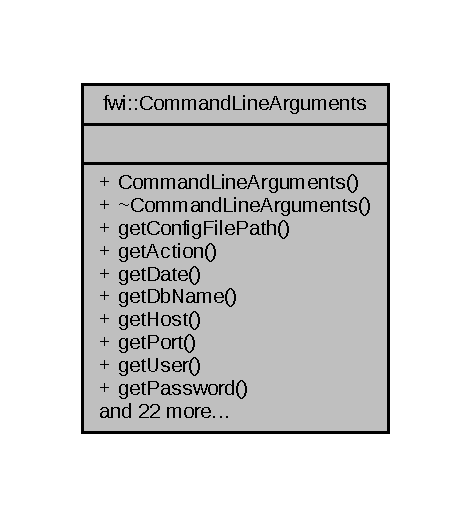
\includegraphics[width=226pt]{classfwi_1_1CommandLineArguments__coll__graph}
\end{center}
\end{figure}
\subsection*{Public Member Functions}
\begin{DoxyCompactItemize}
\item 
\hypertarget{classfwi_1_1CommandLineArguments_a54afbbabb1a2faf818dedb6fc1901c8d}{\hyperlink{classfwi_1_1CommandLineArguments_a54afbbabb1a2faf818dedb6fc1901c8d}{Command\-Line\-Arguments} ()}\label{classfwi_1_1CommandLineArguments_a54afbbabb1a2faf818dedb6fc1901c8d}

\begin{DoxyCompactList}\small\item\em Standard constructor. \end{DoxyCompactList}\item 
\hypertarget{classfwi_1_1CommandLineArguments_a9eee8e8c9b3a12bcab2ff944a233f041}{virtual \hyperlink{classfwi_1_1CommandLineArguments_a9eee8e8c9b3a12bcab2ff944a233f041}{$\sim$\-Command\-Line\-Arguments} ()}\label{classfwi_1_1CommandLineArguments_a9eee8e8c9b3a12bcab2ff944a233f041}

\begin{DoxyCompactList}\small\item\em Destructor. \end{DoxyCompactList}\item 
string \hyperlink{classfwi_1_1CommandLineArguments_a5e55e7e9d3f3ba165a21ead751e1e145}{get\-Config\-File\-Path} () const 
\begin{DoxyCompactList}\small\item\em Config file path getter. \end{DoxyCompactList}\item 
string \hyperlink{classfwi_1_1CommandLineArguments_a744c32d84443793ba21c03959d5f80e2}{get\-Action} () const 
\begin{DoxyCompactList}\small\item\em Action getter. \end{DoxyCompactList}\item 
string \hyperlink{classfwi_1_1CommandLineArguments_a8327187e13b3f2a96cf1becc71c9f68d}{get\-Date} () const 
\begin{DoxyCompactList}\small\item\em Date getter. \end{DoxyCompactList}\item 
string \hyperlink{classfwi_1_1CommandLineArguments_a1813189cfbc370b85ed99f3b9585cebd}{get\-Db\-Name} () const 
\begin{DoxyCompactList}\small\item\em Database name getter. \end{DoxyCompactList}\item 
string \hyperlink{classfwi_1_1CommandLineArguments_a83adbcce0c83237f689b948b8860d3ee}{get\-Host} () const 
\begin{DoxyCompactList}\small\item\em Host getter. \end{DoxyCompactList}\item 
int \hyperlink{classfwi_1_1CommandLineArguments_aed3e2ce12b0d735c219352d16c936afa}{get\-Port} () const 
\begin{DoxyCompactList}\small\item\em Port getter. \end{DoxyCompactList}\item 
string \hyperlink{classfwi_1_1CommandLineArguments_a4aa0d96232454f8ba8445d6474e51b3c}{get\-User} () const 
\begin{DoxyCompactList}\small\item\em User getter. \end{DoxyCompactList}\item 
string \hyperlink{classfwi_1_1CommandLineArguments_a951d2991fe796cc021f64b078a1a55e0}{get\-Password} () const 
\begin{DoxyCompactList}\small\item\em Password getter. \end{DoxyCompactList}\item 
bool \hyperlink{classfwi_1_1CommandLineArguments_a683c730b0b79a90b48dc8596dd994bc4}{get\-Help} () const 
\begin{DoxyCompactList}\small\item\em Help argument presence. \end{DoxyCompactList}\item 
P\-Gconn $\ast$ \hyperlink{classfwi_1_1CommandLineArguments_a071867c84d4756190ddf6e57a2132131}{get\-P\-G\-Connection} (Config \&cfg, bool create=false)
\begin{DoxyCompactList}\small\item\em Gets postgresql connection. \end{DoxyCompactList}\item 
void \hyperlink{classfwi_1_1CommandLineArguments_a31c6f8e8c94e7ca5540c4f84c836f1d3}{close\-P\-G\-Connection} ()
\begin{DoxyCompactList}\small\item\em Gently close postgresql connection. \end{DoxyCompactList}\item 
void \hyperlink{classfwi_1_1CommandLineArguments_ad2548a77ea9819bb6356ffe1ebe2124b}{set\-Config\-File\-Path} (string cfgpath)
\begin{DoxyCompactList}\small\item\em Config\-File\-Path setter. \end{DoxyCompactList}\item 
void \hyperlink{classfwi_1_1CommandLineArguments_a94983023c52fd20932d4e64cf5d566ad}{set\-Action} (string action)
\begin{DoxyCompactList}\small\item\em Action setter. \end{DoxyCompactList}\item 
void \hyperlink{classfwi_1_1CommandLineArguments_af378e847bef06548a276f6ee4ccc72fe}{set\-Date} (string date)
\begin{DoxyCompactList}\small\item\em Date setter. \end{DoxyCompactList}\item 
void \hyperlink{classfwi_1_1CommandLineArguments_a7942eb8218a54ba9843c506396f66f37}{set\-Host} (string host)
\begin{DoxyCompactList}\small\item\em Host setter. \end{DoxyCompactList}\item 
void \hyperlink{classfwi_1_1CommandLineArguments_a624d5a4997b520083b32f589674f4e58}{set\-Db\-Name} (string dbname)
\begin{DoxyCompactList}\small\item\em Database name setter. \end{DoxyCompactList}\item 
void \hyperlink{classfwi_1_1CommandLineArguments_ab283ed9c1d605308f9df2381ec53340e}{set\-Port} (int port)
\begin{DoxyCompactList}\small\item\em Port setter. \end{DoxyCompactList}\item 
void \hyperlink{classfwi_1_1CommandLineArguments_aba8081f570985fba7c0746e4152857a1}{set\-User} (string user)
\begin{DoxyCompactList}\small\item\em User setter. \end{DoxyCompactList}\item 
void \hyperlink{classfwi_1_1CommandLineArguments_af865288c92229fd879333c1d22770f13}{set\-Password} (string password)
\begin{DoxyCompactList}\small\item\em Password setter. \end{DoxyCompactList}\item 
void \hyperlink{classfwi_1_1CommandLineArguments_ab5e55eda6e153cfb3db823366ad72605}{set\-Help} (bool help)
\begin{DoxyCompactList}\small\item\em Help flag setter. \end{DoxyCompactList}\item 
bool \hyperlink{classfwi_1_1CommandLineArguments_a6a2c57edc3311bf3555b6b0a030915e1}{is\-Set\-Action} ()
\begin{DoxyCompactList}\small\item\em Checks for action setting. \end{DoxyCompactList}\item 
bool \hyperlink{classfwi_1_1CommandLineArguments_a582c389cc309b4973a6565dcf5647af3}{is\-Set\-Date} ()
\begin{DoxyCompactList}\small\item\em Checks for date setting. \end{DoxyCompactList}\item 
bool \hyperlink{classfwi_1_1CommandLineArguments_aff14b156dfdadee9a5ae2ba06976ecb0}{is\-Set\-Host} ()
\begin{DoxyCompactList}\small\item\em Checks for host setting. \end{DoxyCompactList}\item 
bool \hyperlink{classfwi_1_1CommandLineArguments_a883bd2b54b445dd1853d8771537fd2c3}{is\-Set\-Db\-Name} ()
\begin{DoxyCompactList}\small\item\em Checks for database name setting. \end{DoxyCompactList}\item 
bool \hyperlink{classfwi_1_1CommandLineArguments_a587ef2a70389522c52277c1aa49f0f22}{is\-Set\-Port} ()
\begin{DoxyCompactList}\small\item\em Checks for port setting. \end{DoxyCompactList}\item 
bool \hyperlink{classfwi_1_1CommandLineArguments_a72d8f5d8be37affd36adc02c7c7f81d6}{is\-Set\-User} ()
\begin{DoxyCompactList}\small\item\em Checks for user setting. \end{DoxyCompactList}\item 
bool \hyperlink{classfwi_1_1CommandLineArguments_a887eaacdc364872e66d8a487ea1f2285}{is\-Set\-Password} ()
\begin{DoxyCompactList}\small\item\em Checks for password setting. \end{DoxyCompactList}\item 
bool \hyperlink{classfwi_1_1CommandLineArguments_acfc136e2da1c2519e94d56ee6b897790}{is\-Set\-Help} ()
\begin{DoxyCompactList}\small\item\em Checks for help setting. \end{DoxyCompactList}\item 
bool \hyperlink{classfwi_1_1CommandLineArguments_a157e286d1dfd5ab7b7ee4e69f85bbc09}{can\-Try\-Db\-Connection} ()
\begin{DoxyCompactList}\small\item\em Checks if a database connection could be done based on current settings. \end{DoxyCompactList}\item 
string \hyperlink{classfwi_1_1CommandLineArguments_aa3f9cdc1eedaf1d795f2921a7ecb6367}{get\-Connection\-String} ()
\begin{DoxyCompactList}\small\item\em Gets the connection string based on current settings. \end{DoxyCompactList}\end{DoxyCompactItemize}


\subsection{Detailed Description}
Command line arguments class. 

\begin{DoxyVerb}     This class stores and manages command line arguments passed to fwidbmgr.<br />
     <h2>fwidbmgr synopsys</h2>
     <i>fwidbmgr -a action [-d date] [-D database] [-H host] [-P port] [-U user] [-p password] [-h]</i><br />
     The possible actions for <b>fwidbmgr</b> are:<br />
     <table border="0">
       <tr><td><b>create</b></td><td>create an empty database structure</td></tr>
       <tr><td><b>createstdgrid</b></td><td>creates the standard 177x174 point grid</td></tr>
       <tr><td><b>fillnometeo</b></td><td>fills nometeo field in standard grid</td></tr>
       <tr><td><b>fillregionmask</b></td><td>fills mask field in standard grid</td></tr>
       <tr><td><b>in</b></td><td>save in db input data for date given by option date</td></tr>
       <tr><td><b>out</b></td><td>save in db output data of fwi indexes computation</td></tr>
       <tr><td><b>outimg</b></td><td>save in db output images</td></tr>
     </table>
\end{DoxyVerb}



\begin{DoxyItemize}
\item {\itshape date} must be a valid date in I\-S\-O 8601 format ex. (2012-\/03-\/22)
\item {\itshape database} is the database name to be used
\item {\itshape host} is the database host name or I\-P address
\item {\itshape port} is the postgresql port
\item {\itshape user} is the database user that has the proper rights
\item {\itshape where} password is the user password

{\bfseries h} --$>$ prints this text 
\end{DoxyItemize}

Definition at line 64 of file Command\-Line\-Arguments.\-h.



\subsection{Member Function Documentation}
\hypertarget{classfwi_1_1CommandLineArguments_a157e286d1dfd5ab7b7ee4e69f85bbc09}{\index{fwi\-::\-Command\-Line\-Arguments@{fwi\-::\-Command\-Line\-Arguments}!can\-Try\-Db\-Connection@{can\-Try\-Db\-Connection}}
\index{can\-Try\-Db\-Connection@{can\-Try\-Db\-Connection}!fwi::CommandLineArguments@{fwi\-::\-Command\-Line\-Arguments}}
\subsubsection[{can\-Try\-Db\-Connection}]{\setlength{\rightskip}{0pt plus 5cm}bool fwi\-::\-Command\-Line\-Arguments\-::can\-Try\-Db\-Connection (
\begin{DoxyParamCaption}
{}
\end{DoxyParamCaption}
)}}\label{classfwi_1_1CommandLineArguments_a157e286d1dfd5ab7b7ee4e69f85bbc09}


Checks if a database connection could be done based on current settings. 

\begin{DoxyReturn}{Returns}
true if can try connection else false 
\end{DoxyReturn}


Definition at line 204 of file Command\-Line\-Arguments.\-cpp.



Here is the caller graph for this function\-:\nopagebreak
\begin{figure}[H]
\begin{center}
\leavevmode
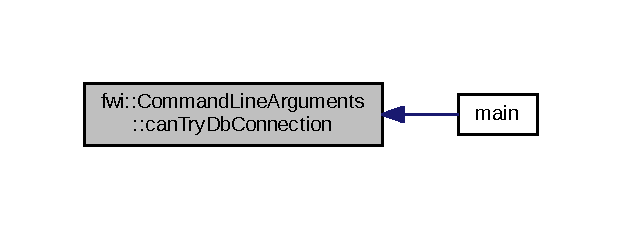
\includegraphics[width=298pt]{classfwi_1_1CommandLineArguments_a157e286d1dfd5ab7b7ee4e69f85bbc09_icgraph}
\end{center}
\end{figure}


\hypertarget{classfwi_1_1CommandLineArguments_a31c6f8e8c94e7ca5540c4f84c836f1d3}{\index{fwi\-::\-Command\-Line\-Arguments@{fwi\-::\-Command\-Line\-Arguments}!close\-P\-G\-Connection@{close\-P\-G\-Connection}}
\index{close\-P\-G\-Connection@{close\-P\-G\-Connection}!fwi::CommandLineArguments@{fwi\-::\-Command\-Line\-Arguments}}
\subsubsection[{close\-P\-G\-Connection}]{\setlength{\rightskip}{0pt plus 5cm}void fwi\-::\-Command\-Line\-Arguments\-::close\-P\-G\-Connection (
\begin{DoxyParamCaption}
{}
\end{DoxyParamCaption}
)}}\label{classfwi_1_1CommandLineArguments_a31c6f8e8c94e7ca5540c4f84c836f1d3}


Gently close postgresql connection. 

\begin{DoxySeeAlso}{See also}
postgresql documentation at \href{http://www.postgresql.org/}{\tt http\-://www.\-postgresql.\-org/} 
\end{DoxySeeAlso}


Definition at line 106 of file Command\-Line\-Arguments.\-cpp.



Here is the caller graph for this function\-:\nopagebreak
\begin{figure}[H]
\begin{center}
\leavevmode
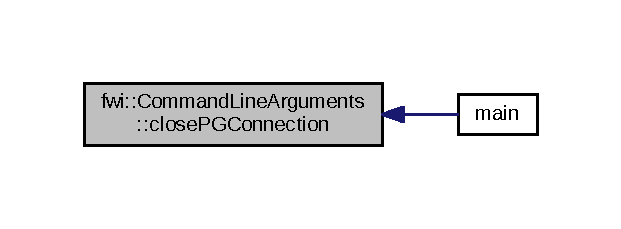
\includegraphics[width=298pt]{classfwi_1_1CommandLineArguments_a31c6f8e8c94e7ca5540c4f84c836f1d3_icgraph}
\end{center}
\end{figure}


\hypertarget{classfwi_1_1CommandLineArguments_a744c32d84443793ba21c03959d5f80e2}{\index{fwi\-::\-Command\-Line\-Arguments@{fwi\-::\-Command\-Line\-Arguments}!get\-Action@{get\-Action}}
\index{get\-Action@{get\-Action}!fwi::CommandLineArguments@{fwi\-::\-Command\-Line\-Arguments}}
\subsubsection[{get\-Action}]{\setlength{\rightskip}{0pt plus 5cm}string fwi\-::\-Command\-Line\-Arguments\-::get\-Action (
\begin{DoxyParamCaption}
{}
\end{DoxyParamCaption}
) const}}\label{classfwi_1_1CommandLineArguments_a744c32d84443793ba21c03959d5f80e2}


Action getter. 

\begin{DoxyReturn}{Returns}
action argument 
\end{DoxyReturn}


Definition at line 43 of file Command\-Line\-Arguments.\-cpp.



Here is the caller graph for this function\-:\nopagebreak
\begin{figure}[H]
\begin{center}
\leavevmode
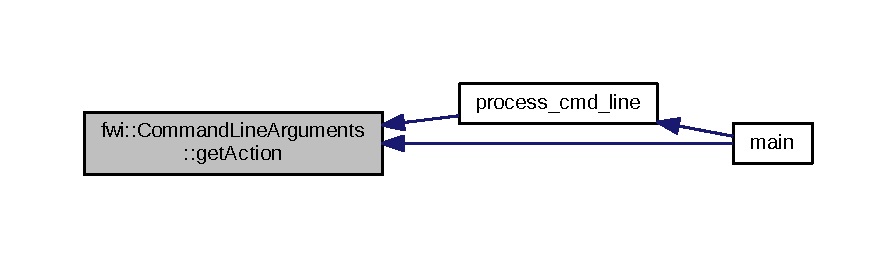
\includegraphics[width=350pt]{classfwi_1_1CommandLineArguments_a744c32d84443793ba21c03959d5f80e2_icgraph}
\end{center}
\end{figure}


\hypertarget{classfwi_1_1CommandLineArguments_a5e55e7e9d3f3ba165a21ead751e1e145}{\index{fwi\-::\-Command\-Line\-Arguments@{fwi\-::\-Command\-Line\-Arguments}!get\-Config\-File\-Path@{get\-Config\-File\-Path}}
\index{get\-Config\-File\-Path@{get\-Config\-File\-Path}!fwi::CommandLineArguments@{fwi\-::\-Command\-Line\-Arguments}}
\subsubsection[{get\-Config\-File\-Path}]{\setlength{\rightskip}{0pt plus 5cm}string fwi\-::\-Command\-Line\-Arguments\-::get\-Config\-File\-Path (
\begin{DoxyParamCaption}
{}
\end{DoxyParamCaption}
) const}}\label{classfwi_1_1CommandLineArguments_a5e55e7e9d3f3ba165a21ead751e1e145}


Config file path getter. 

\begin{DoxyReturn}{Returns}
config\-File\-Path argument 
\end{DoxyReturn}


Definition at line 38 of file Command\-Line\-Arguments.\-cpp.

\hypertarget{classfwi_1_1CommandLineArguments_aa3f9cdc1eedaf1d795f2921a7ecb6367}{\index{fwi\-::\-Command\-Line\-Arguments@{fwi\-::\-Command\-Line\-Arguments}!get\-Connection\-String@{get\-Connection\-String}}
\index{get\-Connection\-String@{get\-Connection\-String}!fwi::CommandLineArguments@{fwi\-::\-Command\-Line\-Arguments}}
\subsubsection[{get\-Connection\-String}]{\setlength{\rightskip}{0pt plus 5cm}string fwi\-::\-Command\-Line\-Arguments\-::get\-Connection\-String (
\begin{DoxyParamCaption}
{}
\end{DoxyParamCaption}
)}}\label{classfwi_1_1CommandLineArguments_aa3f9cdc1eedaf1d795f2921a7ecb6367}


Gets the connection string based on current settings. 

\begin{DoxyReturn}{Returns}
the connection string 
\end{DoxyReturn}


Definition at line 214 of file Command\-Line\-Arguments.\-cpp.

\hypertarget{classfwi_1_1CommandLineArguments_a8327187e13b3f2a96cf1becc71c9f68d}{\index{fwi\-::\-Command\-Line\-Arguments@{fwi\-::\-Command\-Line\-Arguments}!get\-Date@{get\-Date}}
\index{get\-Date@{get\-Date}!fwi::CommandLineArguments@{fwi\-::\-Command\-Line\-Arguments}}
\subsubsection[{get\-Date}]{\setlength{\rightskip}{0pt plus 5cm}string fwi\-::\-Command\-Line\-Arguments\-::get\-Date (
\begin{DoxyParamCaption}
{}
\end{DoxyParamCaption}
) const}}\label{classfwi_1_1CommandLineArguments_a8327187e13b3f2a96cf1becc71c9f68d}


Date getter. 

\begin{DoxyReturn}{Returns}
date argument 
\end{DoxyReturn}


Definition at line 48 of file Command\-Line\-Arguments.\-cpp.



Here is the caller graph for this function\-:
\nopagebreak
\begin{figure}[H]
\begin{center}
\leavevmode
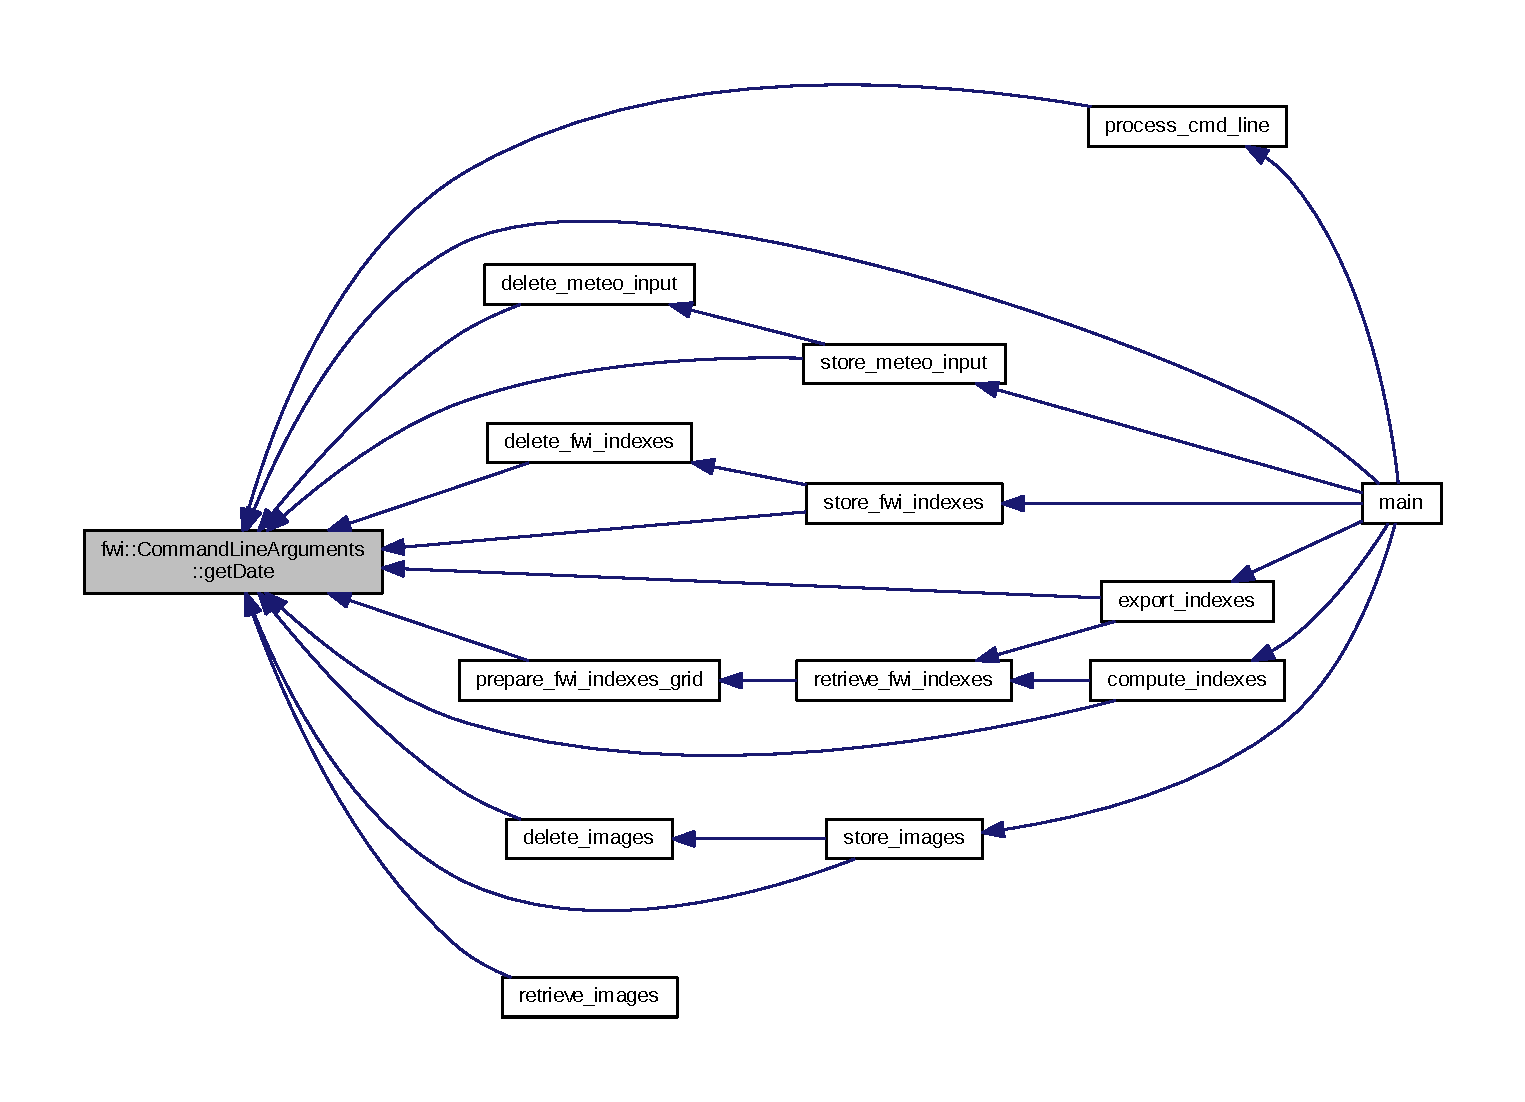
\includegraphics[width=350pt]{classfwi_1_1CommandLineArguments_a8327187e13b3f2a96cf1becc71c9f68d_icgraph}
\end{center}
\end{figure}


\hypertarget{classfwi_1_1CommandLineArguments_a1813189cfbc370b85ed99f3b9585cebd}{\index{fwi\-::\-Command\-Line\-Arguments@{fwi\-::\-Command\-Line\-Arguments}!get\-Db\-Name@{get\-Db\-Name}}
\index{get\-Db\-Name@{get\-Db\-Name}!fwi::CommandLineArguments@{fwi\-::\-Command\-Line\-Arguments}}
\subsubsection[{get\-Db\-Name}]{\setlength{\rightskip}{0pt plus 5cm}string fwi\-::\-Command\-Line\-Arguments\-::get\-Db\-Name (
\begin{DoxyParamCaption}
{}
\end{DoxyParamCaption}
) const}}\label{classfwi_1_1CommandLineArguments_a1813189cfbc370b85ed99f3b9585cebd}


Database name getter. 

\begin{DoxyReturn}{Returns}
database name argument 
\end{DoxyReturn}


Definition at line 53 of file Command\-Line\-Arguments.\-cpp.



Here is the caller graph for this function\-:\nopagebreak
\begin{figure}[H]
\begin{center}
\leavevmode
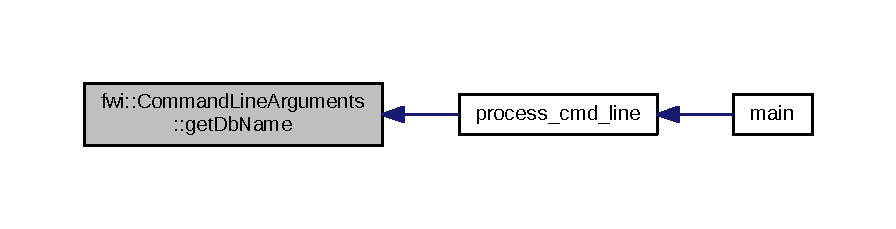
\includegraphics[width=350pt]{classfwi_1_1CommandLineArguments_a1813189cfbc370b85ed99f3b9585cebd_icgraph}
\end{center}
\end{figure}


\hypertarget{classfwi_1_1CommandLineArguments_a683c730b0b79a90b48dc8596dd994bc4}{\index{fwi\-::\-Command\-Line\-Arguments@{fwi\-::\-Command\-Line\-Arguments}!get\-Help@{get\-Help}}
\index{get\-Help@{get\-Help}!fwi::CommandLineArguments@{fwi\-::\-Command\-Line\-Arguments}}
\subsubsection[{get\-Help}]{\setlength{\rightskip}{0pt plus 5cm}bool fwi\-::\-Command\-Line\-Arguments\-::get\-Help (
\begin{DoxyParamCaption}
{}
\end{DoxyParamCaption}
) const}}\label{classfwi_1_1CommandLineArguments_a683c730b0b79a90b48dc8596dd994bc4}


Help argument presence. 

\begin{DoxyReturn}{Returns}
true help argument passed to program else false 
\end{DoxyReturn}


Definition at line 78 of file Command\-Line\-Arguments.\-cpp.

\hypertarget{classfwi_1_1CommandLineArguments_a83adbcce0c83237f689b948b8860d3ee}{\index{fwi\-::\-Command\-Line\-Arguments@{fwi\-::\-Command\-Line\-Arguments}!get\-Host@{get\-Host}}
\index{get\-Host@{get\-Host}!fwi::CommandLineArguments@{fwi\-::\-Command\-Line\-Arguments}}
\subsubsection[{get\-Host}]{\setlength{\rightskip}{0pt plus 5cm}string fwi\-::\-Command\-Line\-Arguments\-::get\-Host (
\begin{DoxyParamCaption}
{}
\end{DoxyParamCaption}
) const}}\label{classfwi_1_1CommandLineArguments_a83adbcce0c83237f689b948b8860d3ee}


Host getter. 

\begin{DoxyReturn}{Returns}
host argument 
\end{DoxyReturn}


Definition at line 58 of file Command\-Line\-Arguments.\-cpp.



Here is the caller graph for this function\-:\nopagebreak
\begin{figure}[H]
\begin{center}
\leavevmode
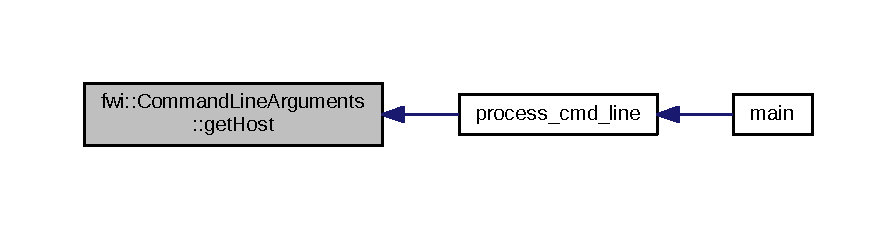
\includegraphics[width=350pt]{classfwi_1_1CommandLineArguments_a83adbcce0c83237f689b948b8860d3ee_icgraph}
\end{center}
\end{figure}


\hypertarget{classfwi_1_1CommandLineArguments_a951d2991fe796cc021f64b078a1a55e0}{\index{fwi\-::\-Command\-Line\-Arguments@{fwi\-::\-Command\-Line\-Arguments}!get\-Password@{get\-Password}}
\index{get\-Password@{get\-Password}!fwi::CommandLineArguments@{fwi\-::\-Command\-Line\-Arguments}}
\subsubsection[{get\-Password}]{\setlength{\rightskip}{0pt plus 5cm}string fwi\-::\-Command\-Line\-Arguments\-::get\-Password (
\begin{DoxyParamCaption}
{}
\end{DoxyParamCaption}
) const}}\label{classfwi_1_1CommandLineArguments_a951d2991fe796cc021f64b078a1a55e0}


Password getter. 

\begin{DoxyReturn}{Returns}
password argument 
\end{DoxyReturn}


Definition at line 63 of file Command\-Line\-Arguments.\-cpp.

\hypertarget{classfwi_1_1CommandLineArguments_a071867c84d4756190ddf6e57a2132131}{\index{fwi\-::\-Command\-Line\-Arguments@{fwi\-::\-Command\-Line\-Arguments}!get\-P\-G\-Connection@{get\-P\-G\-Connection}}
\index{get\-P\-G\-Connection@{get\-P\-G\-Connection}!fwi::CommandLineArguments@{fwi\-::\-Command\-Line\-Arguments}}
\subsubsection[{get\-P\-G\-Connection}]{\setlength{\rightskip}{0pt plus 5cm}P\-Gconn $\ast$ fwi\-::\-Command\-Line\-Arguments\-::get\-P\-G\-Connection (
\begin{DoxyParamCaption}
\item[{Config \&}]{cfg, }
\item[{bool}]{create = {\ttfamily false}}
\end{DoxyParamCaption}
)}}\label{classfwi_1_1CommandLineArguments_a071867c84d4756190ddf6e57a2132131}


Gets postgresql connection. 


\begin{DoxyParams}{Parameters}
{\em cfg} & configuration class from libconfig++ \\
\hline
{\em create} & if true create a new connection \\
\hline
\end{DoxyParams}
\begin{DoxyReturn}{Returns}
postgresql connection 
\end{DoxyReturn}
\begin{DoxySeeAlso}{See also}
libconfig++ documentation at \href{http://www.hyperrealm.com/libconfig/}{\tt http\-://www.\-hyperrealm.\-com/libconfig/} 

postgresql documentation at \href{http://www.postgresql.org/}{\tt http\-://www.\-postgresql.\-org/} 
\end{DoxySeeAlso}


Definition at line 83 of file Command\-Line\-Arguments.\-cpp.



Here is the caller graph for this function\-:\nopagebreak
\begin{figure}[H]
\begin{center}
\leavevmode
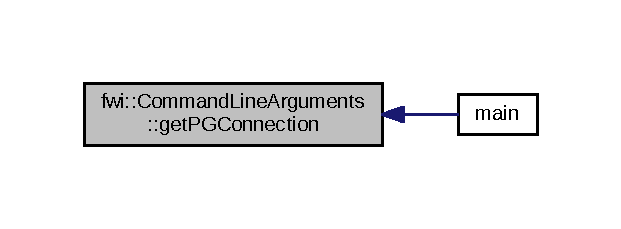
\includegraphics[width=298pt]{classfwi_1_1CommandLineArguments_a071867c84d4756190ddf6e57a2132131_icgraph}
\end{center}
\end{figure}


\hypertarget{classfwi_1_1CommandLineArguments_aed3e2ce12b0d735c219352d16c936afa}{\index{fwi\-::\-Command\-Line\-Arguments@{fwi\-::\-Command\-Line\-Arguments}!get\-Port@{get\-Port}}
\index{get\-Port@{get\-Port}!fwi::CommandLineArguments@{fwi\-::\-Command\-Line\-Arguments}}
\subsubsection[{get\-Port}]{\setlength{\rightskip}{0pt plus 5cm}int fwi\-::\-Command\-Line\-Arguments\-::get\-Port (
\begin{DoxyParamCaption}
{}
\end{DoxyParamCaption}
) const}}\label{classfwi_1_1CommandLineArguments_aed3e2ce12b0d735c219352d16c936afa}


Port getter. 

\begin{DoxyReturn}{Returns}
port argument 
\end{DoxyReturn}


Definition at line 68 of file Command\-Line\-Arguments.\-cpp.



Here is the caller graph for this function\-:\nopagebreak
\begin{figure}[H]
\begin{center}
\leavevmode
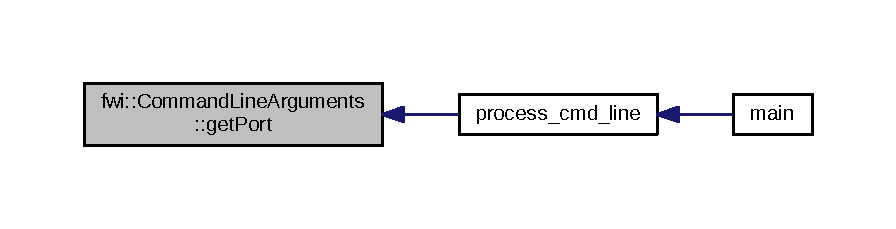
\includegraphics[width=350pt]{classfwi_1_1CommandLineArguments_aed3e2ce12b0d735c219352d16c936afa_icgraph}
\end{center}
\end{figure}


\hypertarget{classfwi_1_1CommandLineArguments_a4aa0d96232454f8ba8445d6474e51b3c}{\index{fwi\-::\-Command\-Line\-Arguments@{fwi\-::\-Command\-Line\-Arguments}!get\-User@{get\-User}}
\index{get\-User@{get\-User}!fwi::CommandLineArguments@{fwi\-::\-Command\-Line\-Arguments}}
\subsubsection[{get\-User}]{\setlength{\rightskip}{0pt plus 5cm}string fwi\-::\-Command\-Line\-Arguments\-::get\-User (
\begin{DoxyParamCaption}
{}
\end{DoxyParamCaption}
) const}}\label{classfwi_1_1CommandLineArguments_a4aa0d96232454f8ba8445d6474e51b3c}


User getter. 

\begin{DoxyReturn}{Returns}
user argument 
\end{DoxyReturn}


Definition at line 73 of file Command\-Line\-Arguments.\-cpp.



Here is the caller graph for this function\-:\nopagebreak
\begin{figure}[H]
\begin{center}
\leavevmode
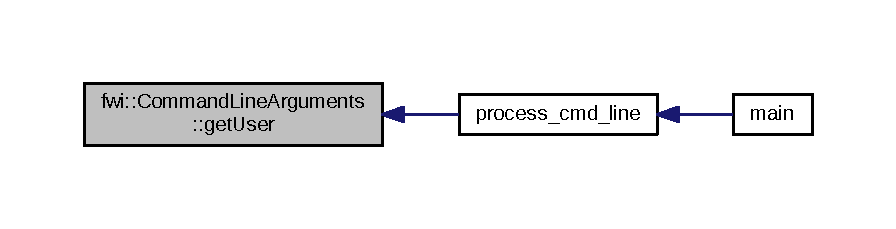
\includegraphics[width=350pt]{classfwi_1_1CommandLineArguments_a4aa0d96232454f8ba8445d6474e51b3c_icgraph}
\end{center}
\end{figure}


\hypertarget{classfwi_1_1CommandLineArguments_a6a2c57edc3311bf3555b6b0a030915e1}{\index{fwi\-::\-Command\-Line\-Arguments@{fwi\-::\-Command\-Line\-Arguments}!is\-Set\-Action@{is\-Set\-Action}}
\index{is\-Set\-Action@{is\-Set\-Action}!fwi::CommandLineArguments@{fwi\-::\-Command\-Line\-Arguments}}
\subsubsection[{is\-Set\-Action}]{\setlength{\rightskip}{0pt plus 5cm}bool fwi\-::\-Command\-Line\-Arguments\-::is\-Set\-Action (
\begin{DoxyParamCaption}
{}
\end{DoxyParamCaption}
)}}\label{classfwi_1_1CommandLineArguments_a6a2c57edc3311bf3555b6b0a030915e1}


Checks for action setting. 

\begin{DoxyReturn}{Returns}
true if action is set else false 
\end{DoxyReturn}


Definition at line 160 of file Command\-Line\-Arguments.\-cpp.

\hypertarget{classfwi_1_1CommandLineArguments_a582c389cc309b4973a6565dcf5647af3}{\index{fwi\-::\-Command\-Line\-Arguments@{fwi\-::\-Command\-Line\-Arguments}!is\-Set\-Date@{is\-Set\-Date}}
\index{is\-Set\-Date@{is\-Set\-Date}!fwi::CommandLineArguments@{fwi\-::\-Command\-Line\-Arguments}}
\subsubsection[{is\-Set\-Date}]{\setlength{\rightskip}{0pt plus 5cm}bool fwi\-::\-Command\-Line\-Arguments\-::is\-Set\-Date (
\begin{DoxyParamCaption}
{}
\end{DoxyParamCaption}
)}}\label{classfwi_1_1CommandLineArguments_a582c389cc309b4973a6565dcf5647af3}


Checks for date setting. 

\begin{DoxyReturn}{Returns}
true if date is set else false 
\end{DoxyReturn}


Definition at line 165 of file Command\-Line\-Arguments.\-cpp.



Here is the caller graph for this function\-:\nopagebreak
\begin{figure}[H]
\begin{center}
\leavevmode
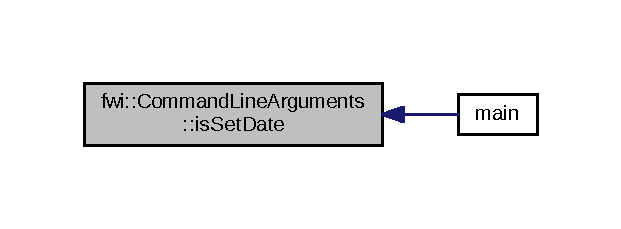
\includegraphics[width=298pt]{classfwi_1_1CommandLineArguments_a582c389cc309b4973a6565dcf5647af3_icgraph}
\end{center}
\end{figure}


\hypertarget{classfwi_1_1CommandLineArguments_a883bd2b54b445dd1853d8771537fd2c3}{\index{fwi\-::\-Command\-Line\-Arguments@{fwi\-::\-Command\-Line\-Arguments}!is\-Set\-Db\-Name@{is\-Set\-Db\-Name}}
\index{is\-Set\-Db\-Name@{is\-Set\-Db\-Name}!fwi::CommandLineArguments@{fwi\-::\-Command\-Line\-Arguments}}
\subsubsection[{is\-Set\-Db\-Name}]{\setlength{\rightskip}{0pt plus 5cm}bool fwi\-::\-Command\-Line\-Arguments\-::is\-Set\-Db\-Name (
\begin{DoxyParamCaption}
{}
\end{DoxyParamCaption}
)}}\label{classfwi_1_1CommandLineArguments_a883bd2b54b445dd1853d8771537fd2c3}


Checks for database name setting. 

\begin{DoxyReturn}{Returns}
true if database name is set else false 
\end{DoxyReturn}


Definition at line 175 of file Command\-Line\-Arguments.\-cpp.



Here is the caller graph for this function\-:\nopagebreak
\begin{figure}[H]
\begin{center}
\leavevmode
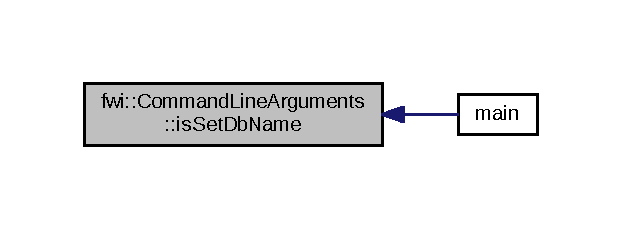
\includegraphics[width=298pt]{classfwi_1_1CommandLineArguments_a883bd2b54b445dd1853d8771537fd2c3_icgraph}
\end{center}
\end{figure}


\hypertarget{classfwi_1_1CommandLineArguments_acfc136e2da1c2519e94d56ee6b897790}{\index{fwi\-::\-Command\-Line\-Arguments@{fwi\-::\-Command\-Line\-Arguments}!is\-Set\-Help@{is\-Set\-Help}}
\index{is\-Set\-Help@{is\-Set\-Help}!fwi::CommandLineArguments@{fwi\-::\-Command\-Line\-Arguments}}
\subsubsection[{is\-Set\-Help}]{\setlength{\rightskip}{0pt plus 5cm}bool fwi\-::\-Command\-Line\-Arguments\-::is\-Set\-Help (
\begin{DoxyParamCaption}
{}
\end{DoxyParamCaption}
)}}\label{classfwi_1_1CommandLineArguments_acfc136e2da1c2519e94d56ee6b897790}


Checks for help setting. 

\begin{DoxyReturn}{Returns}
true if help is set else false 
\end{DoxyReturn}


Definition at line 195 of file Command\-Line\-Arguments.\-cpp.



Here is the caller graph for this function\-:\nopagebreak
\begin{figure}[H]
\begin{center}
\leavevmode
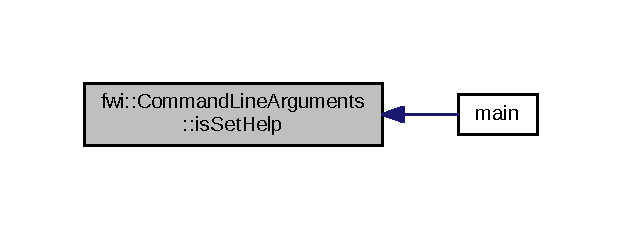
\includegraphics[width=298pt]{classfwi_1_1CommandLineArguments_acfc136e2da1c2519e94d56ee6b897790_icgraph}
\end{center}
\end{figure}


\hypertarget{classfwi_1_1CommandLineArguments_aff14b156dfdadee9a5ae2ba06976ecb0}{\index{fwi\-::\-Command\-Line\-Arguments@{fwi\-::\-Command\-Line\-Arguments}!is\-Set\-Host@{is\-Set\-Host}}
\index{is\-Set\-Host@{is\-Set\-Host}!fwi::CommandLineArguments@{fwi\-::\-Command\-Line\-Arguments}}
\subsubsection[{is\-Set\-Host}]{\setlength{\rightskip}{0pt plus 5cm}bool fwi\-::\-Command\-Line\-Arguments\-::is\-Set\-Host (
\begin{DoxyParamCaption}
{}
\end{DoxyParamCaption}
)}}\label{classfwi_1_1CommandLineArguments_aff14b156dfdadee9a5ae2ba06976ecb0}


Checks for host setting. 

\begin{DoxyReturn}{Returns}
true if host is set else false 
\end{DoxyReturn}


Definition at line 170 of file Command\-Line\-Arguments.\-cpp.



Here is the caller graph for this function\-:\nopagebreak
\begin{figure}[H]
\begin{center}
\leavevmode
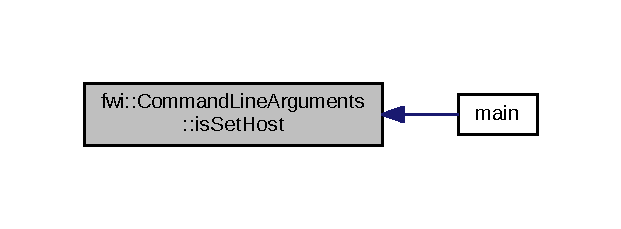
\includegraphics[width=298pt]{classfwi_1_1CommandLineArguments_aff14b156dfdadee9a5ae2ba06976ecb0_icgraph}
\end{center}
\end{figure}


\hypertarget{classfwi_1_1CommandLineArguments_a887eaacdc364872e66d8a487ea1f2285}{\index{fwi\-::\-Command\-Line\-Arguments@{fwi\-::\-Command\-Line\-Arguments}!is\-Set\-Password@{is\-Set\-Password}}
\index{is\-Set\-Password@{is\-Set\-Password}!fwi::CommandLineArguments@{fwi\-::\-Command\-Line\-Arguments}}
\subsubsection[{is\-Set\-Password}]{\setlength{\rightskip}{0pt plus 5cm}bool fwi\-::\-Command\-Line\-Arguments\-::is\-Set\-Password (
\begin{DoxyParamCaption}
{}
\end{DoxyParamCaption}
)}}\label{classfwi_1_1CommandLineArguments_a887eaacdc364872e66d8a487ea1f2285}


Checks for password setting. 

\begin{DoxyReturn}{Returns}
true if password is set else false 
\end{DoxyReturn}


Definition at line 180 of file Command\-Line\-Arguments.\-cpp.



Here is the caller graph for this function\-:\nopagebreak
\begin{figure}[H]
\begin{center}
\leavevmode
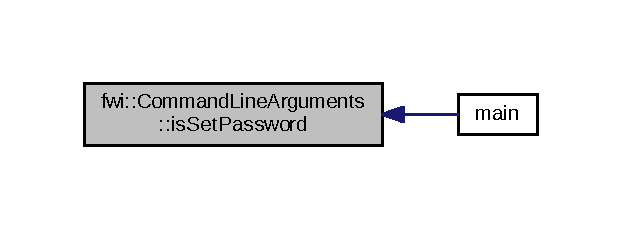
\includegraphics[width=298pt]{classfwi_1_1CommandLineArguments_a887eaacdc364872e66d8a487ea1f2285_icgraph}
\end{center}
\end{figure}


\hypertarget{classfwi_1_1CommandLineArguments_a587ef2a70389522c52277c1aa49f0f22}{\index{fwi\-::\-Command\-Line\-Arguments@{fwi\-::\-Command\-Line\-Arguments}!is\-Set\-Port@{is\-Set\-Port}}
\index{is\-Set\-Port@{is\-Set\-Port}!fwi::CommandLineArguments@{fwi\-::\-Command\-Line\-Arguments}}
\subsubsection[{is\-Set\-Port}]{\setlength{\rightskip}{0pt plus 5cm}bool fwi\-::\-Command\-Line\-Arguments\-::is\-Set\-Port (
\begin{DoxyParamCaption}
{}
\end{DoxyParamCaption}
)}}\label{classfwi_1_1CommandLineArguments_a587ef2a70389522c52277c1aa49f0f22}


Checks for port setting. 

\begin{DoxyReturn}{Returns}
true if port is set else false 
\end{DoxyReturn}


Definition at line 185 of file Command\-Line\-Arguments.\-cpp.



Here is the caller graph for this function\-:\nopagebreak
\begin{figure}[H]
\begin{center}
\leavevmode
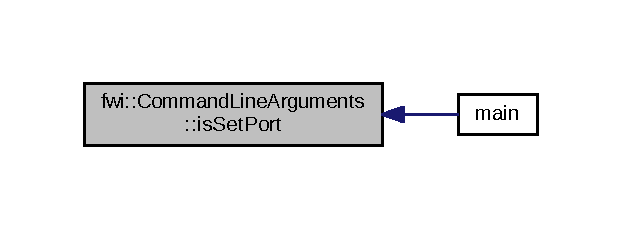
\includegraphics[width=298pt]{classfwi_1_1CommandLineArguments_a587ef2a70389522c52277c1aa49f0f22_icgraph}
\end{center}
\end{figure}


\hypertarget{classfwi_1_1CommandLineArguments_a72d8f5d8be37affd36adc02c7c7f81d6}{\index{fwi\-::\-Command\-Line\-Arguments@{fwi\-::\-Command\-Line\-Arguments}!is\-Set\-User@{is\-Set\-User}}
\index{is\-Set\-User@{is\-Set\-User}!fwi::CommandLineArguments@{fwi\-::\-Command\-Line\-Arguments}}
\subsubsection[{is\-Set\-User}]{\setlength{\rightskip}{0pt plus 5cm}bool fwi\-::\-Command\-Line\-Arguments\-::is\-Set\-User (
\begin{DoxyParamCaption}
{}
\end{DoxyParamCaption}
)}}\label{classfwi_1_1CommandLineArguments_a72d8f5d8be37affd36adc02c7c7f81d6}


Checks for user setting. 

\begin{DoxyReturn}{Returns}
true if user is set else false 
\end{DoxyReturn}


Definition at line 190 of file Command\-Line\-Arguments.\-cpp.



Here is the caller graph for this function\-:\nopagebreak
\begin{figure}[H]
\begin{center}
\leavevmode
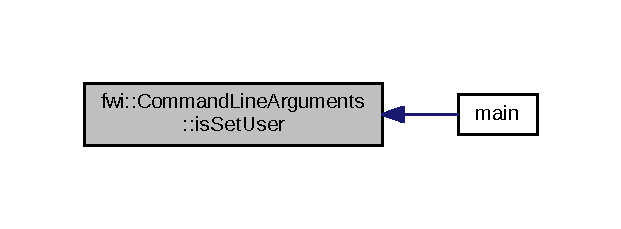
\includegraphics[width=298pt]{classfwi_1_1CommandLineArguments_a72d8f5d8be37affd36adc02c7c7f81d6_icgraph}
\end{center}
\end{figure}


\hypertarget{classfwi_1_1CommandLineArguments_a94983023c52fd20932d4e64cf5d566ad}{\index{fwi\-::\-Command\-Line\-Arguments@{fwi\-::\-Command\-Line\-Arguments}!set\-Action@{set\-Action}}
\index{set\-Action@{set\-Action}!fwi::CommandLineArguments@{fwi\-::\-Command\-Line\-Arguments}}
\subsubsection[{set\-Action}]{\setlength{\rightskip}{0pt plus 5cm}void fwi\-::\-Command\-Line\-Arguments\-::set\-Action (
\begin{DoxyParamCaption}
\item[{string}]{action}
\end{DoxyParamCaption}
)}}\label{classfwi_1_1CommandLineArguments_a94983023c52fd20932d4e64cf5d566ad}


Action setter. 


\begin{DoxyParams}{Parameters}
{\em action} & action to set \\
\hline
\end{DoxyParams}


Definition at line 120 of file Command\-Line\-Arguments.\-cpp.



Here is the caller graph for this function\-:\nopagebreak
\begin{figure}[H]
\begin{center}
\leavevmode
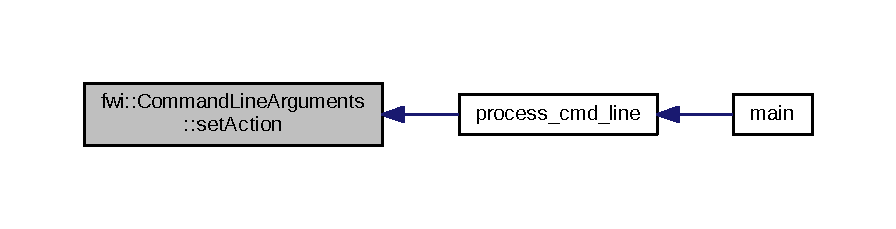
\includegraphics[width=350pt]{classfwi_1_1CommandLineArguments_a94983023c52fd20932d4e64cf5d566ad_icgraph}
\end{center}
\end{figure}


\hypertarget{classfwi_1_1CommandLineArguments_ad2548a77ea9819bb6356ffe1ebe2124b}{\index{fwi\-::\-Command\-Line\-Arguments@{fwi\-::\-Command\-Line\-Arguments}!set\-Config\-File\-Path@{set\-Config\-File\-Path}}
\index{set\-Config\-File\-Path@{set\-Config\-File\-Path}!fwi::CommandLineArguments@{fwi\-::\-Command\-Line\-Arguments}}
\subsubsection[{set\-Config\-File\-Path}]{\setlength{\rightskip}{0pt plus 5cm}void fwi\-::\-Command\-Line\-Arguments\-::set\-Config\-File\-Path (
\begin{DoxyParamCaption}
\item[{string}]{cfgpath}
\end{DoxyParamCaption}
)}}\label{classfwi_1_1CommandLineArguments_ad2548a77ea9819bb6356ffe1ebe2124b}


Config\-File\-Path setter. 


\begin{DoxyParams}{Parameters}
{\em cfgpath} & config\-File\-Path to set \\
\hline
\end{DoxyParams}


Definition at line 115 of file Command\-Line\-Arguments.\-cpp.

\hypertarget{classfwi_1_1CommandLineArguments_af378e847bef06548a276f6ee4ccc72fe}{\index{fwi\-::\-Command\-Line\-Arguments@{fwi\-::\-Command\-Line\-Arguments}!set\-Date@{set\-Date}}
\index{set\-Date@{set\-Date}!fwi::CommandLineArguments@{fwi\-::\-Command\-Line\-Arguments}}
\subsubsection[{set\-Date}]{\setlength{\rightskip}{0pt plus 5cm}void fwi\-::\-Command\-Line\-Arguments\-::set\-Date (
\begin{DoxyParamCaption}
\item[{string}]{date}
\end{DoxyParamCaption}
)}}\label{classfwi_1_1CommandLineArguments_af378e847bef06548a276f6ee4ccc72fe}


Date setter. 


\begin{DoxyParams}{Parameters}
{\em date} & date to set \\
\hline
\end{DoxyParams}


Definition at line 125 of file Command\-Line\-Arguments.\-cpp.



Here is the caller graph for this function\-:\nopagebreak
\begin{figure}[H]
\begin{center}
\leavevmode
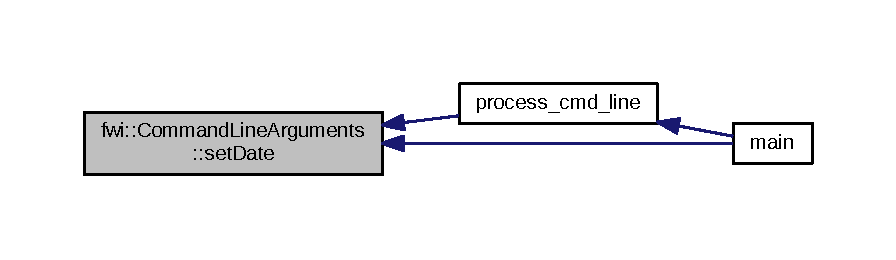
\includegraphics[width=350pt]{classfwi_1_1CommandLineArguments_af378e847bef06548a276f6ee4ccc72fe_icgraph}
\end{center}
\end{figure}


\hypertarget{classfwi_1_1CommandLineArguments_a624d5a4997b520083b32f589674f4e58}{\index{fwi\-::\-Command\-Line\-Arguments@{fwi\-::\-Command\-Line\-Arguments}!set\-Db\-Name@{set\-Db\-Name}}
\index{set\-Db\-Name@{set\-Db\-Name}!fwi::CommandLineArguments@{fwi\-::\-Command\-Line\-Arguments}}
\subsubsection[{set\-Db\-Name}]{\setlength{\rightskip}{0pt plus 5cm}void fwi\-::\-Command\-Line\-Arguments\-::set\-Db\-Name (
\begin{DoxyParamCaption}
\item[{string}]{dbname}
\end{DoxyParamCaption}
)}}\label{classfwi_1_1CommandLineArguments_a624d5a4997b520083b32f589674f4e58}


Database name setter. 


\begin{DoxyParams}{Parameters}
{\em dbname} & databasee name to set \\
\hline
\end{DoxyParams}


Definition at line 130 of file Command\-Line\-Arguments.\-cpp.



Here is the caller graph for this function\-:\nopagebreak
\begin{figure}[H]
\begin{center}
\leavevmode
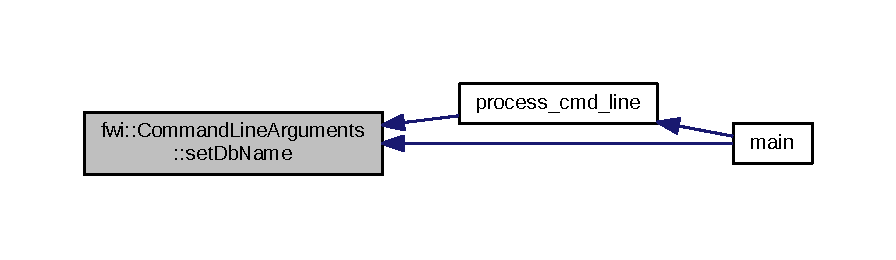
\includegraphics[width=350pt]{classfwi_1_1CommandLineArguments_a624d5a4997b520083b32f589674f4e58_icgraph}
\end{center}
\end{figure}


\hypertarget{classfwi_1_1CommandLineArguments_ab5e55eda6e153cfb3db823366ad72605}{\index{fwi\-::\-Command\-Line\-Arguments@{fwi\-::\-Command\-Line\-Arguments}!set\-Help@{set\-Help}}
\index{set\-Help@{set\-Help}!fwi::CommandLineArguments@{fwi\-::\-Command\-Line\-Arguments}}
\subsubsection[{set\-Help}]{\setlength{\rightskip}{0pt plus 5cm}void fwi\-::\-Command\-Line\-Arguments\-::set\-Help (
\begin{DoxyParamCaption}
\item[{bool}]{help}
\end{DoxyParamCaption}
)}}\label{classfwi_1_1CommandLineArguments_ab5e55eda6e153cfb3db823366ad72605}


Help flag setter. 


\begin{DoxyParams}{Parameters}
{\em help} & help flag to set \\
\hline
\end{DoxyParams}


Definition at line 155 of file Command\-Line\-Arguments.\-cpp.



Here is the caller graph for this function\-:\nopagebreak
\begin{figure}[H]
\begin{center}
\leavevmode
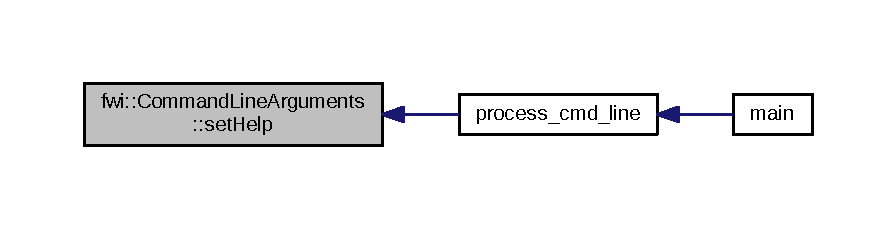
\includegraphics[width=350pt]{classfwi_1_1CommandLineArguments_ab5e55eda6e153cfb3db823366ad72605_icgraph}
\end{center}
\end{figure}


\hypertarget{classfwi_1_1CommandLineArguments_a7942eb8218a54ba9843c506396f66f37}{\index{fwi\-::\-Command\-Line\-Arguments@{fwi\-::\-Command\-Line\-Arguments}!set\-Host@{set\-Host}}
\index{set\-Host@{set\-Host}!fwi::CommandLineArguments@{fwi\-::\-Command\-Line\-Arguments}}
\subsubsection[{set\-Host}]{\setlength{\rightskip}{0pt plus 5cm}void fwi\-::\-Command\-Line\-Arguments\-::set\-Host (
\begin{DoxyParamCaption}
\item[{string}]{host}
\end{DoxyParamCaption}
)}}\label{classfwi_1_1CommandLineArguments_a7942eb8218a54ba9843c506396f66f37}


Host setter. 


\begin{DoxyParams}{Parameters}
{\em host} & host to set \\
\hline
\end{DoxyParams}


Definition at line 135 of file Command\-Line\-Arguments.\-cpp.



Here is the caller graph for this function\-:\nopagebreak
\begin{figure}[H]
\begin{center}
\leavevmode
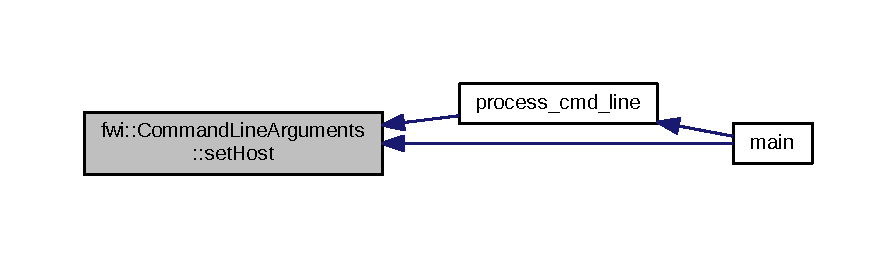
\includegraphics[width=350pt]{classfwi_1_1CommandLineArguments_a7942eb8218a54ba9843c506396f66f37_icgraph}
\end{center}
\end{figure}


\hypertarget{classfwi_1_1CommandLineArguments_af865288c92229fd879333c1d22770f13}{\index{fwi\-::\-Command\-Line\-Arguments@{fwi\-::\-Command\-Line\-Arguments}!set\-Password@{set\-Password}}
\index{set\-Password@{set\-Password}!fwi::CommandLineArguments@{fwi\-::\-Command\-Line\-Arguments}}
\subsubsection[{set\-Password}]{\setlength{\rightskip}{0pt plus 5cm}void fwi\-::\-Command\-Line\-Arguments\-::set\-Password (
\begin{DoxyParamCaption}
\item[{string}]{password}
\end{DoxyParamCaption}
)}}\label{classfwi_1_1CommandLineArguments_af865288c92229fd879333c1d22770f13}


Password setter. 


\begin{DoxyParams}{Parameters}
{\em password} & password to set \\
\hline
\end{DoxyParams}


Definition at line 140 of file Command\-Line\-Arguments.\-cpp.



Here is the caller graph for this function\-:\nopagebreak
\begin{figure}[H]
\begin{center}
\leavevmode
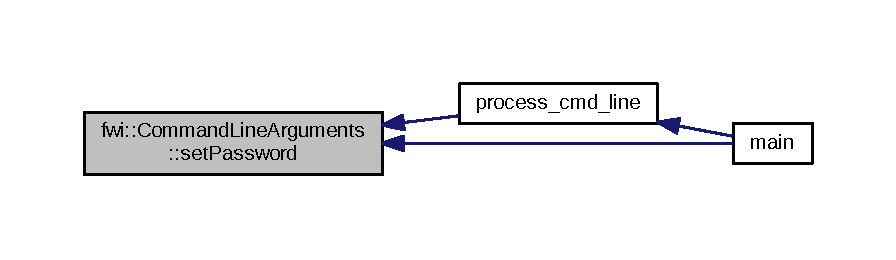
\includegraphics[width=350pt]{classfwi_1_1CommandLineArguments_af865288c92229fd879333c1d22770f13_icgraph}
\end{center}
\end{figure}


\hypertarget{classfwi_1_1CommandLineArguments_ab283ed9c1d605308f9df2381ec53340e}{\index{fwi\-::\-Command\-Line\-Arguments@{fwi\-::\-Command\-Line\-Arguments}!set\-Port@{set\-Port}}
\index{set\-Port@{set\-Port}!fwi::CommandLineArguments@{fwi\-::\-Command\-Line\-Arguments}}
\subsubsection[{set\-Port}]{\setlength{\rightskip}{0pt plus 5cm}void fwi\-::\-Command\-Line\-Arguments\-::set\-Port (
\begin{DoxyParamCaption}
\item[{int}]{port}
\end{DoxyParamCaption}
)}}\label{classfwi_1_1CommandLineArguments_ab283ed9c1d605308f9df2381ec53340e}


Port setter. 


\begin{DoxyParams}{Parameters}
{\em port} & port to set \\
\hline
\end{DoxyParams}


Definition at line 145 of file Command\-Line\-Arguments.\-cpp.



Here is the caller graph for this function\-:\nopagebreak
\begin{figure}[H]
\begin{center}
\leavevmode
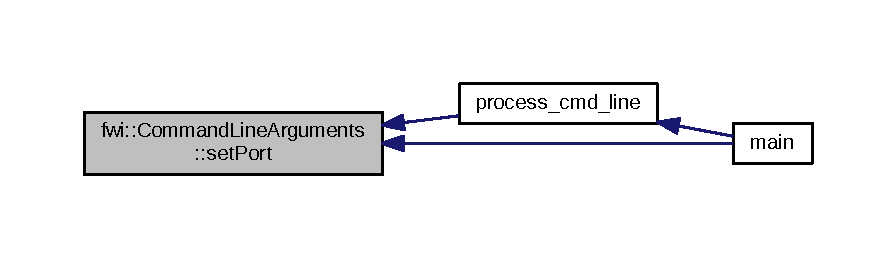
\includegraphics[width=350pt]{classfwi_1_1CommandLineArguments_ab283ed9c1d605308f9df2381ec53340e_icgraph}
\end{center}
\end{figure}


\hypertarget{classfwi_1_1CommandLineArguments_aba8081f570985fba7c0746e4152857a1}{\index{fwi\-::\-Command\-Line\-Arguments@{fwi\-::\-Command\-Line\-Arguments}!set\-User@{set\-User}}
\index{set\-User@{set\-User}!fwi::CommandLineArguments@{fwi\-::\-Command\-Line\-Arguments}}
\subsubsection[{set\-User}]{\setlength{\rightskip}{0pt plus 5cm}void fwi\-::\-Command\-Line\-Arguments\-::set\-User (
\begin{DoxyParamCaption}
\item[{string}]{user}
\end{DoxyParamCaption}
)}}\label{classfwi_1_1CommandLineArguments_aba8081f570985fba7c0746e4152857a1}


User setter. 


\begin{DoxyParams}{Parameters}
{\em user} & user to set \\
\hline
\end{DoxyParams}


Definition at line 150 of file Command\-Line\-Arguments.\-cpp.



Here is the caller graph for this function\-:\nopagebreak
\begin{figure}[H]
\begin{center}
\leavevmode
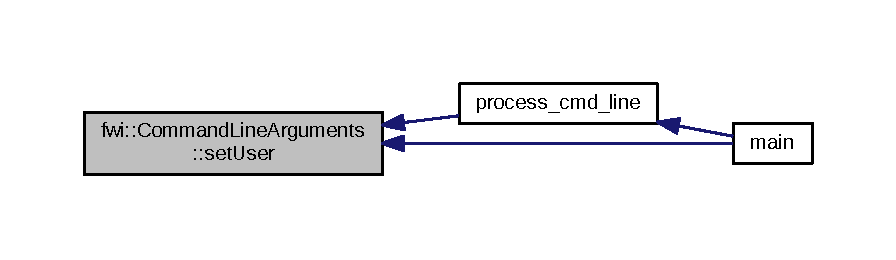
\includegraphics[width=350pt]{classfwi_1_1CommandLineArguments_aba8081f570985fba7c0746e4152857a1_icgraph}
\end{center}
\end{figure}




The documentation for this class was generated from the following files\-:\begin{DoxyCompactItemize}
\item 
include/\hyperlink{CommandLineArguments_8h}{Command\-Line\-Arguments.\-h}\item 
src/\hyperlink{CommandLineArguments_8cpp}{Command\-Line\-Arguments.\-cpp}\end{DoxyCompactItemize}

\hypertarget{classfwi_1_1grid_1_1Grid}{\section{fwi\-:\-:grid\-:\-:Grid$<$ T $>$ Class Template Reference}
\label{classfwi_1_1grid_1_1Grid}\index{fwi\-::grid\-::\-Grid$<$ T $>$@{fwi\-::grid\-::\-Grid$<$ T $>$}}
}


3-\/dimensional grid  




{\ttfamily \#include $<$Grid.\-h$>$}



Collaboration diagram for fwi\-:\-:grid\-:\-:Grid$<$ T $>$\-:
\nopagebreak
\begin{figure}[H]
\begin{center}
\leavevmode
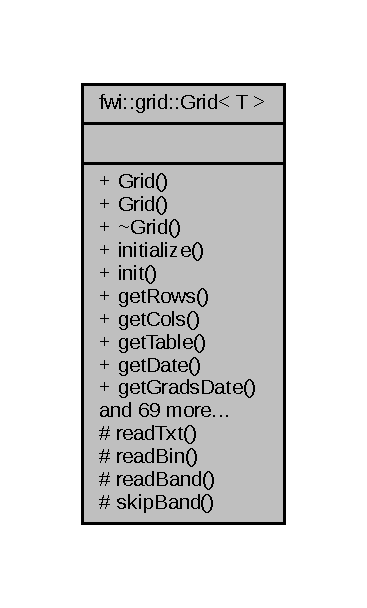
\includegraphics[width=176pt]{classfwi_1_1grid_1_1Grid__coll__graph}
\end{center}
\end{figure}
\subsection*{Public Types}
\begin{DoxyCompactItemize}
\item 
\hypertarget{classfwi_1_1grid_1_1Grid_a890011022f243b72633d7bc28fa7494e}{typedef grid\-\_\-t\-::index \hyperlink{classfwi_1_1grid_1_1Grid_a890011022f243b72633d7bc28fa7494e}{index}}\label{classfwi_1_1grid_1_1Grid_a890011022f243b72633d7bc28fa7494e}

\begin{DoxyCompactList}\small\item\em typedef helper \end{DoxyCompactList}\end{DoxyCompactItemize}
\subsection*{Public Member Functions}
\begin{DoxyCompactItemize}
\item 
\hypertarget{classfwi_1_1grid_1_1Grid_a1328a3f31a8b8fb007597dfd6bcf1cbd}{\hyperlink{classfwi_1_1grid_1_1Grid_a1328a3f31a8b8fb007597dfd6bcf1cbd}{Grid} (int varnum=\hyperlink{fwi__define_8h_a0b5ef1a7f011a268d5767ad76dc0d2f3}{G\-R\-D\-\_\-\-D\-E\-F\-A\-U\-L\-T\-\_\-\-V\-A\-R\-N\-U\-M})}\label{classfwi_1_1grid_1_1Grid_a1328a3f31a8b8fb007597dfd6bcf1cbd}

\begin{DoxyCompactList}\small\item\em Standard constructor. \end{DoxyCompactList}\item 
\hyperlink{classfwi_1_1grid_1_1Grid_aa3834cf6b13445bf8eb53b6ebe1cfb71}{Grid} (int rows, int cols, std\-::string table=\hyperlink{fwi__define_8h_a2a3ae53495ee4efc3c35a2acc837603c}{G\-R\-D\-\_\-\-D\-E\-F\-A\-U\-L\-T\-\_\-\-T\-A\-B\-L\-E}, int type=\hyperlink{fwi__define_8h_aea937ca2785273f5b96467b2b3f3d22d}{G\-E\-O\-G\-R\-I\-D}, float xstart=\hyperlink{fwi__define_8h_aba5ceb4d7323417c50fdc179ce915020}{G\-R\-D\-\_\-\-X\-\_\-\-S\-T\-A\-R\-T}, float ystart=\hyperlink{fwi__define_8h_a08e286b41c7e537fde7ecebff1c59ce3}{G\-R\-D\-\_\-\-Y\-\_\-\-S\-T\-A\-R\-T}, float xstep=\hyperlink{fwi__define_8h_ab0465700b128a48e19c72d90119a96e1}{G\-R\-D\-\_\-\-X\-\_\-\-S\-T\-E\-P}, float ystep=\hyperlink{fwi__define_8h_a3b5df539b73755a7159b0e38bc69ce7a}{G\-R\-D\-\_\-\-Y\-\_\-\-S\-T\-E\-P}, C\-O\-O\-R\-D\-I\-N\-A\-T\-E\-\_\-\-D\-I\-R\-E\-C\-T\-I\-O\-N xdir=I\-N\-C\-R\-E\-A\-S\-I\-N\-G, C\-O\-O\-R\-D\-I\-N\-A\-T\-E\-\_\-\-D\-I\-R\-E\-C\-T\-I\-O\-N ydir=I\-N\-C\-R\-E\-A\-S\-I\-N\-G, int varnum=\hyperlink{fwi__define_8h_a0b5ef1a7f011a268d5767ad76dc0d2f3}{G\-R\-D\-\_\-\-D\-E\-F\-A\-U\-L\-T\-\_\-\-V\-A\-R\-N\-U\-M}, int srid=\hyperlink{fwi__define_8h_a039f584144fef5765f3541a17f8dc3c4}{G\-I\-S\-\_\-\-D\-E\-F\-A\-U\-L\-T\-\_\-\-S\-R\-I\-D}, float undef\-Value=\hyperlink{fwi__define_8h_a7682eceef088f1177c13859d3d7ce43d}{G\-R\-D\-\_\-\-D\-E\-F\-A\-U\-L\-T\-\_\-\-U\-N\-D\-E\-F\-\_\-\-V\-A\-L\-U\-E}, int slot\-Size=G\-R\-D\-\_\-\-D\-E\-F\-A\-U\-L\-T\-\_\-\-S\-L\-O\-T\-S\-I\-Z\-E)
\begin{DoxyCompactList}\small\item\em Parameterized constructor. \end{DoxyCompactList}\item 
\hypertarget{classfwi_1_1grid_1_1Grid_af9301a4e3301edfe6faf65d71a563037}{virtual \hyperlink{classfwi_1_1grid_1_1Grid_af9301a4e3301edfe6faf65d71a563037}{$\sim$\-Grid} ()}\label{classfwi_1_1grid_1_1Grid_af9301a4e3301edfe6faf65d71a563037}

\begin{DoxyCompactList}\small\item\em Destructor. \end{DoxyCompactList}\item 
\hypertarget{classfwi_1_1grid_1_1Grid_a546028acbdac7d1646e7f3ede24c76b9}{void \hyperlink{classfwi_1_1grid_1_1Grid_a546028acbdac7d1646e7f3ede24c76b9}{initialize} ()}\label{classfwi_1_1grid_1_1Grid_a546028acbdac7d1646e7f3ede24c76b9}

\begin{DoxyCompactList}\small\item\em Initialize grid memory. \end{DoxyCompactList}\item 
\hypertarget{classfwi_1_1grid_1_1Grid_a15090d3154d2f147b6437464354d9c20}{void \hyperlink{classfwi_1_1grid_1_1Grid_a15090d3154d2f147b6437464354d9c20}{init} (T t)}\label{classfwi_1_1grid_1_1Grid_a15090d3154d2f147b6437464354d9c20}

\begin{DoxyCompactList}\small\item\em set all grid elements to t \end{DoxyCompactList}\item 
int \hyperlink{classfwi_1_1grid_1_1Grid_a7c43b6bb6f6b0d61a6669bd5c7ea8c7a}{get\-Rows} () const 
\begin{DoxyCompactList}\small\item\em rows number getter \end{DoxyCompactList}\item 
int \hyperlink{classfwi_1_1grid_1_1Grid_aaf9b9814c8f513ceba002b75542620c9}{get\-Cols} () const 
\begin{DoxyCompactList}\small\item\em cols number getter \end{DoxyCompactList}\item 
std\-::string \hyperlink{classfwi_1_1grid_1_1Grid_afc3fafe3429aa908a9af84674dc4c1ee}{get\-Table} () const 
\begin{DoxyCompactList}\small\item\em grid database table name getter \end{DoxyCompactList}\item 
std\-::string \hyperlink{classfwi_1_1grid_1_1Grid_ac7c89b5eb43447e86ea0b5b956a8b88d}{get\-Date} () const 
\begin{DoxyCompactList}\small\item\em date getter \end{DoxyCompactList}\item 
std\-::string \hyperlink{classfwi_1_1grid_1_1Grid_a51a7b639a01826dc7437d646930f6891}{get\-Grads\-Date} () const 
\begin{DoxyCompactList}\small\item\em date in Gr\-A\-D\-S format getter \end{DoxyCompactList}\item 
std\-::string \hyperlink{classfwi_1_1grid_1_1Grid_a4be1b06ee3d8c6a4eabdd3a402ae3bf9}{get\-Ctl\-Path} () const 
\begin{DoxyCompactList}\small\item\em grid ctl file path getter \end{DoxyCompactList}\item 
std\-::string \hyperlink{classfwi_1_1grid_1_1Grid_a23e0a0d0fa907ccfbc0881240dc528a2}{get\-Dat\-Path} () const 
\begin{DoxyCompactList}\small\item\em grid dat file path getter \end{DoxyCompactList}\item 
std\-::string \hyperlink{classfwi_1_1grid_1_1Grid_a4fdc08766fd405bd37d38a6709c08342}{get\-Export\-Dat\-Path} () const 
\begin{DoxyCompactList}\small\item\em grid export dat file path getter \end{DoxyCompactList}\item 
std\-::string \hyperlink{classfwi_1_1grid_1_1Grid_a2a47f95c96985a5e639285bde471d9a5}{get\-Export\-Ctl\-Path} () const 
\begin{DoxyCompactList}\small\item\em grid export ctl file path getter \end{DoxyCompactList}\item 
std\-::string \hyperlink{classfwi_1_1grid_1_1Grid_a7e9e12dc12588d1834c261b610cac319}{get\-Title} () const 
\begin{DoxyCompactList}\small\item\em grid title getter \end{DoxyCompactList}\item 
int \hyperlink{classfwi_1_1grid_1_1Grid_a2deb54df5fc5e90b3b5b061a516c2a92}{get\-Type} () const 
\begin{DoxyCompactList}\small\item\em grid type getter \end{DoxyCompactList}\item 
int \hyperlink{classfwi_1_1grid_1_1Grid_ae9043ae6499a47872c6161516b721e21}{get\-Time\-Band} () const 
\begin{DoxyCompactList}\small\item\em grid time band \end{DoxyCompactList}\item 
int \hyperlink{classfwi_1_1grid_1_1Grid_ac6f053b3983bf2f651a1a523b8591be4}{get\-Time\-Bands\-Number} () const 
\begin{DoxyCompactList}\small\item\em grid time bands number \end{DoxyCompactList}\item 
std\-::string \hyperlink{classfwi_1_1grid_1_1Grid_a869002c87fc7e935b66c40ea712b90e4}{get\-Start\-Time} () const 
\begin{DoxyCompactList}\small\item\em grid start time getter \end{DoxyCompactList}\item 
std\-::string \hyperlink{classfwi_1_1grid_1_1Grid_aa6a35277617cbae5fe3db3f9ae28558d}{get\-Time\-Increment} () const 
\begin{DoxyCompactList}\small\item\em grid time increment getter \end{DoxyCompactList}\item 
int \hyperlink{classfwi_1_1grid_1_1Grid_ac8b97200a77c83bbed7c441fe8414212}{get\-File\-Name\-Date\-Offset} () const 
\begin{DoxyCompactList}\small\item\em grid file name date offset getter \end{DoxyCompactList}\item 
int \hyperlink{classfwi_1_1grid_1_1Grid_af6127c6adeb24967516c1d9e0af1a4c6}{get\-I\-O\-Format} () const 
\begin{DoxyCompactList}\small\item\em grid I/\-O format getter \end{DoxyCompactList}\item 
float \hyperlink{classfwi_1_1grid_1_1Grid_ae2feb145847b2504ca2474a9e3e33945}{get\-X\-Start} () const 
\begin{DoxyCompactList}\small\item\em grid start x coordinate getter \end{DoxyCompactList}\item 
float \hyperlink{classfwi_1_1grid_1_1Grid_ac2986f115fadf2ef16cf0b9e61114baf}{get\-X\-Step} () const 
\begin{DoxyCompactList}\small\item\em grid step in x direction getter \end{DoxyCompactList}\item 
float \hyperlink{classfwi_1_1grid_1_1Grid_a5e41f9d7886b318044b1de323d075d54}{get\-Y\-Start} () const 
\begin{DoxyCompactList}\small\item\em grid start y coordinate getter \end{DoxyCompactList}\item 
float \hyperlink{classfwi_1_1grid_1_1Grid_aae81a8e8fddf00750337a86bc6940337}{get\-Y\-Step} () const 
\begin{DoxyCompactList}\small\item\em grid step in y direction getter \end{DoxyCompactList}\item 
C\-O\-O\-R\-D\-I\-N\-A\-T\-E\-\_\-\-D\-I\-R\-E\-C\-T\-I\-O\-N \hyperlink{classfwi_1_1grid_1_1Grid_a60d11b4f03f3ed4ef4349d25897486d7}{get\-X\-Dir} () const 
\begin{DoxyCompactList}\small\item\em x\-Dir getter \end{DoxyCompactList}\item 
C\-O\-O\-R\-D\-I\-N\-A\-T\-E\-\_\-\-D\-I\-R\-E\-C\-T\-I\-O\-N \hyperlink{classfwi_1_1grid_1_1Grid_ac8761c50efb6f2af694727b9b12d9f0e}{get\-Y\-Dir} () const 
\begin{DoxyCompactList}\small\item\em y\-Dir getter \end{DoxyCompactList}\item 
int \hyperlink{classfwi_1_1grid_1_1Grid_ad9e9ac91e9c338606e1199ffa89fc6bb}{get\-Var\-Num} () const 
\begin{DoxyCompactList}\small\item\em variables number getter \end{DoxyCompactList}\item 
int \hyperlink{classfwi_1_1grid_1_1Grid_a8aefb75a246d3a618f455d34c7e64f3f}{get\-S\-R\-I\-D} () const 
\begin{DoxyCompactList}\small\item\em grid srid getter \end{DoxyCompactList}\item 
float \hyperlink{classfwi_1_1grid_1_1Grid_a8d18ce74846ea7432f034a30ef879b59}{get\-Undef\-Value} () const 
\begin{DoxyCompactList}\small\item\em grid undefindined value getter \end{DoxyCompactList}\item 
int \hyperlink{classfwi_1_1grid_1_1Grid_adf68e16a1b1d07ed1745c57eb6732314}{get\-Slot\-Size} () const 
\begin{DoxyCompactList}\small\item\em grid slot size getter \end{DoxyCompactList}\item 
grid\-\_\-t \hyperlink{classfwi_1_1grid_1_1Grid_a73e900020a90dbad3808d3c91778a3b4}{get\-Data} ()
\begin{DoxyCompactList}\small\item\em grid internal data pointer getter \end{DoxyCompactList}\item 
\hyperlink{classfwi_1_1grid_1_1GridFields}{Grid\-Fields} $\ast$ \hyperlink{classfwi_1_1grid_1_1Grid_a2e891ed3f46840241652cd435ac35a94}{get\-Fields} () const 
\begin{DoxyCompactList}\small\item\em grid fields list getter \end{DoxyCompactList}\item 
int \hyperlink{classfwi_1_1grid_1_1Grid_abe660314639e862657818d02aad3ff45}{get\-Elements\-Count} ()
\begin{DoxyCompactList}\small\item\em gets the element count as rows x cols \end{DoxyCompactList}\item 
int \hyperlink{classfwi_1_1grid_1_1Grid_aa140c12f1edfb152b7e859488969cf3e}{get\-Total\-Elements\-Count} ()
\begin{DoxyCompactList}\small\item\em gets the total element count as rows x cols x var\-Num \end{DoxyCompactList}\item 
void \hyperlink{classfwi_1_1grid_1_1Grid_aefe04321df7e26e6510293846d93f983}{set\-Rows} (int rows)
\begin{DoxyCompactList}\small\item\em grid rows number setter \end{DoxyCompactList}\item 
void \hyperlink{classfwi_1_1grid_1_1Grid_a8ee0c76d69626d72bc385c5cb3cdf268}{set\-Cols} (int cols)
\begin{DoxyCompactList}\small\item\em grid columns number setter \end{DoxyCompactList}\item 
void \hyperlink{classfwi_1_1grid_1_1Grid_a78f4a38e86a245ee62769e5f37bff1c6}{set\-Table} (std\-::string table)
\begin{DoxyCompactList}\small\item\em grid table name setter \end{DoxyCompactList}\item 
void \hyperlink{classfwi_1_1grid_1_1Grid_a38c849794390871a95b8c7dbe505e00d}{set\-Date} (std\-::string date)
\begin{DoxyCompactList}\small\item\em date setter \end{DoxyCompactList}\item 
void \hyperlink{classfwi_1_1grid_1_1Grid_a5beeb3bf022ee1dec908f76bf1b7ff5d}{set\-Ctl\-Path} (std\-::string filepath)
\begin{DoxyCompactList}\small\item\em grid ctl file path setter \end{DoxyCompactList}\item 
void \hyperlink{classfwi_1_1grid_1_1Grid_ac7df5d5cc5b9d184c5eceb03737bb598}{set\-Dat\-Path} (std\-::string filepath)
\begin{DoxyCompactList}\small\item\em grid dat file path setter \end{DoxyCompactList}\item 
void \hyperlink{classfwi_1_1grid_1_1Grid_ab138cac6c49037fc1b911a7a7d2eb437}{set\-Export\-Ctl\-Path} (std\-::string filepath)
\begin{DoxyCompactList}\small\item\em grid export ctl file path setter \end{DoxyCompactList}\item 
void \hyperlink{classfwi_1_1grid_1_1Grid_a84899af1e9496f79a7cf43459c62c9bc}{set\-Export\-Dat\-Path} (std\-::string filepath)
\begin{DoxyCompactList}\small\item\em grid export dat file path setter \end{DoxyCompactList}\item 
void \hyperlink{classfwi_1_1grid_1_1Grid_a0cdb2357ad4279db9bc990bb17eecef0}{set\-Title} (std\-::string title)
\begin{DoxyCompactList}\small\item\em grid title setter \end{DoxyCompactList}\item 
void \hyperlink{classfwi_1_1grid_1_1Grid_a6e7dc5bcf9d26a25289a324b2d4f8926}{set\-Type} (int type)
\begin{DoxyCompactList}\small\item\em grid type setter \end{DoxyCompactList}\item 
void \hyperlink{classfwi_1_1grid_1_1Grid_a3ed06b6c1a2ea5596c78256b2b872d81}{set\-Time\-Band} (int band)
\begin{DoxyCompactList}\small\item\em grid time band setter \end{DoxyCompactList}\item 
void \hyperlink{classfwi_1_1grid_1_1Grid_a19b83ec99e6280c7da1ad6b08cc3b921}{set\-Time\-Bands\-Number} (int bands\-Number)
\begin{DoxyCompactList}\small\item\em grid time bands number setter \end{DoxyCompactList}\item 
void \hyperlink{classfwi_1_1grid_1_1Grid_a9e75d99eef25e9a401aadd71ad646e08}{set\-Start\-Time} (std\-::string t)
\begin{DoxyCompactList}\small\item\em grid start time setter \end{DoxyCompactList}\item 
void \hyperlink{classfwi_1_1grid_1_1Grid_afc7b78751770989300220237fcae5256}{set\-Time\-Increment} (std\-::string increment)
\begin{DoxyCompactList}\small\item\em grid time increment setter \end{DoxyCompactList}\item 
void \hyperlink{classfwi_1_1grid_1_1Grid_a15e1fd1e87919bba2971a6fe66566f43}{set\-File\-Name\-Date\-Offset} (int offset)
\begin{DoxyCompactList}\small\item\em grid file name date offset setter \end{DoxyCompactList}\item 
void \hyperlink{classfwi_1_1grid_1_1Grid_a4fe86c25ec42f48f70d2353721e9aeed}{set\-I\-O\-Format} (int format)
\begin{DoxyCompactList}\small\item\em grid I/\-O format setter \end{DoxyCompactList}\item 
void \hyperlink{classfwi_1_1grid_1_1Grid_a3e358d51e63374a9174fcff2206ba9d1}{set\-X\-Start} (float xstart)
\begin{DoxyCompactList}\small\item\em grid start x coordinate setter \end{DoxyCompactList}\item 
void \hyperlink{classfwi_1_1grid_1_1Grid_a442147db5a15cb302bc640041bc42d49}{set\-X\-Step} (float xstep)
\begin{DoxyCompactList}\small\item\em grid step in x direction setter \end{DoxyCompactList}\item 
void \hyperlink{classfwi_1_1grid_1_1Grid_a9a22e6a8991396d957900b33b9db6558}{set\-Y\-Start} (float ystart)
\begin{DoxyCompactList}\small\item\em grid start y coordinate setter \end{DoxyCompactList}\item 
void \hyperlink{classfwi_1_1grid_1_1Grid_aeb84b8b6061243f47f6cea19bda8acbc}{set\-Y\-Step} (float ystep)
\begin{DoxyCompactList}\small\item\em grid step in y direction setter \end{DoxyCompactList}\item 
void \hyperlink{classfwi_1_1grid_1_1Grid_a58a313c74d268e1a892877dbe97782e0}{set\-X\-Dir} (C\-O\-O\-R\-D\-I\-N\-A\-T\-E\-\_\-\-D\-I\-R\-E\-C\-T\-I\-O\-N x\-Dir)
\begin{DoxyCompactList}\small\item\em x\-Dir setter \end{DoxyCompactList}\item 
void \hyperlink{classfwi_1_1grid_1_1Grid_a8ee82188e306a47c14813024513bd56e}{set\-Y\-Dir} (C\-O\-O\-R\-D\-I\-N\-A\-T\-E\-\_\-\-D\-I\-R\-E\-C\-T\-I\-O\-N y\-Dir)
\begin{DoxyCompactList}\small\item\em y\-Dir setter \end{DoxyCompactList}\item 
void \hyperlink{classfwi_1_1grid_1_1Grid_ab063dbc1b9e23f21c27611851390de23}{set\-Var\-Num} (int varnum)
\begin{DoxyCompactList}\small\item\em grid variables number setter \end{DoxyCompactList}\item 
void \hyperlink{classfwi_1_1grid_1_1Grid_aff98dae08698282b2a1661810856e673}{set\-S\-R\-I\-D} (int srid)
\begin{DoxyCompactList}\small\item\em grid srid setter \end{DoxyCompactList}\item 
void \hyperlink{classfwi_1_1grid_1_1Grid_ad1090e0ab615bf979eb72bbc55ca6fb3}{set\-Undef\-Value} (float undef\-Value)
\begin{DoxyCompactList}\small\item\em grid undefined value setter \end{DoxyCompactList}\item 
void \hyperlink{classfwi_1_1grid_1_1Grid_ac0fe4e20d56ed5507f62c1d3e6502f68}{set\-Slot\-Size} (int slot\-Size)
\begin{DoxyCompactList}\small\item\em grid slot size setter \end{DoxyCompactList}\item 
void \hyperlink{classfwi_1_1grid_1_1Grid_acfa22cf6901ee071064d5dccc255f5ed}{set\-Fields} (\hyperlink{classfwi_1_1grid_1_1GridFields}{Grid\-Fields} $\ast$fields)
\begin{DoxyCompactList}\small\item\em grid fields list setter \end{DoxyCompactList}\item 
T \& \hyperlink{classfwi_1_1grid_1_1Grid_a4892438084efa099f29fbb4fbf5d3e83}{operator()} (int i, int j, int k)
\begin{DoxyCompactList}\small\item\em grid element access helper \end{DoxyCompactList}\item 
\hyperlink{classfwi_1_1grid_1_1Grid}{Grid}$<$ T $>$ \& \hyperlink{classfwi_1_1grid_1_1Grid_a8cbde1277dbb531069c1b579cb10410f}{operator=} (const \hyperlink{classfwi_1_1grid_1_1Grid}{Grid}$<$ T $>$ \&grid)
\begin{DoxyCompactList}\small\item\em grid assignement operator \end{DoxyCompactList}\item 
\hypertarget{classfwi_1_1grid_1_1Grid_a9e1229aefd4781e60641e1a946fb64e3}{void \hyperlink{classfwi_1_1grid_1_1Grid_a9e1229aefd4781e60641e1a946fb64e3}{raw\-\_\-dump} ()}\label{classfwi_1_1grid_1_1Grid_a9e1229aefd4781e60641e1a946fb64e3}

\begin{DoxyCompactList}\small\item\em raw dump helper \end{DoxyCompactList}\item 
bool \hyperlink{classfwi_1_1grid_1_1Grid_abfcac51edc50447a1861ce85d68409cf}{configure} (std\-::string name, Config \&cfg)
\begin{DoxyCompactList}\small\item\em configure grid from config file \end{DoxyCompactList}\item 
bool \hyperlink{classfwi_1_1grid_1_1Grid_a254a6c5a649b7d3a109f67811ef5f356}{merge} (\hyperlink{classfwi_1_1grid_1_1Grid}{Grid}$<$ T $>$ \&other)
\begin{DoxyCompactList}\small\item\em merges {\itshape other} whith {\bfseries this} \end{DoxyCompactList}\item 
bool \hyperlink{classfwi_1_1grid_1_1Grid_a099e8895d70f6ce5a5eba5ea3599704f}{subgrid} (std\-::vector$<$ std\-::string $>$ fieldnames, \hyperlink{classfwi_1_1grid_1_1Grid}{Grid}$<$ T $>$ \&sg)
\begin{DoxyCompactList}\small\item\em Extracts a subgrid from {\itshape this} having fields contained in {\itshape fieldnames} \end{DoxyCompactList}\item 
bool \hyperlink{classfwi_1_1grid_1_1Grid_a34cc464d768d11a63f6918e6a39e0415}{read\-Ctrl} (ifstream \&in)
\begin{DoxyCompactList}\small\item\em reads grid control file \end{DoxyCompactList}\item 
bool \hyperlink{classfwi_1_1grid_1_1Grid_aafc829b90cb1a0dc6ec9daf425f6b8b7}{read} ()
\begin{DoxyCompactList}\small\item\em reads grid binary file \end{DoxyCompactList}\item 
bool \hyperlink{classfwi_1_1grid_1_1Grid_a115667cd2987c5972d7fa28d0f07a008}{write\-Ctrl} (ofstream \&out)
\begin{DoxyCompactList}\small\item\em write grid ctl file \end{DoxyCompactList}\item 
bool \hyperlink{classfwi_1_1grid_1_1Grid_a3288da25df63b739516c2bf90f9131fa}{write} (ofstream \&out)
\begin{DoxyCompactList}\small\item\em writes grid binary file \end{DoxyCompactList}\item 
bool \hyperlink{classfwi_1_1grid_1_1Grid_a0f7797bf1413a6082559ce7d4561ecbc}{write\-Txt} (ofstream \&out, bool esri=false)
\begin{DoxyCompactList}\small\item\em writes grid text file \end{DoxyCompactList}\item 
bool \hyperlink{classfwi_1_1grid_1_1Grid_ac3ac1ccceb7696f022d39ca4e99e5b92}{stored} (P\-Gconn $\ast$conn)
\begin{DoxyCompactList}\small\item\em verify if {\bfseries this} is already stored in database \end{DoxyCompactList}\item 
bool \hyperlink{classfwi_1_1grid_1_1Grid_ad440bf48610e89a053d5d1a32a28579a}{store} (P\-Gconn $\ast$conn)
\begin{DoxyCompactList}\small\item\em stores grid in database \end{DoxyCompactList}\item 
bool \hyperlink{classfwi_1_1grid_1_1Grid_a65a165655dd630f5f1b7c52b4e261059}{insert} (P\-Gconn $\ast$conn)
\begin{DoxyCompactList}\small\item\em insert grid in database \end{DoxyCompactList}\item 
bool \hyperlink{classfwi_1_1grid_1_1Grid_ac255d83afc8e784761cb2d46775612ee}{update} (P\-Gconn $\ast$conn)
\begin{DoxyCompactList}\small\item\em updates grid in database \end{DoxyCompactList}\item 
bool \hyperlink{classfwi_1_1grid_1_1Grid_a653fc4a3630fbcfc92229b42fea9ab77}{retrieve} (P\-Gconn $\ast$conn)
\begin{DoxyCompactList}\small\item\em retrieves grid from database \end{DoxyCompactList}\end{DoxyCompactItemize}
\subsection*{Protected Member Functions}
\begin{DoxyCompactItemize}
\item 
bool \hyperlink{classfwi_1_1grid_1_1Grid_ac6262b427ff75bcfac1d118afccb1c71}{read\-Txt} (ifstream \&in)
\begin{DoxyCompactList}\small\item\em reads grid data from text file \end{DoxyCompactList}\item 
bool \hyperlink{classfwi_1_1grid_1_1Grid_a9f941bf44e6f27620181cd7b406150e2}{read\-Bin} (ifstream \&in)
\begin{DoxyCompactList}\small\item\em reads grid data from binary file \end{DoxyCompactList}\item 
bool \hyperlink{classfwi_1_1grid_1_1Grid_a07cf7c55e15a35e7b258574a8cda7685}{read\-Band} (ifstream \&in)
\begin{DoxyCompactList}\small\item\em reads data from a grid time band (stream must be opened in binary mode) not appliable to text streams \end{DoxyCompactList}\item 
void \hyperlink{classfwi_1_1grid_1_1Grid_a4b7534ee12c05e1a492da8de36cc0751}{skip\-Band} (ifstream \&in)
\begin{DoxyCompactList}\small\item\em skip the next timeband from reading \end{DoxyCompactList}\end{DoxyCompactItemize}
\subsection*{Friends}
\begin{DoxyCompactItemize}
\item 
\hypertarget{classfwi_1_1grid_1_1Grid_a3d70a0064502ecd7311f33a9bd4ab742}{ostream \& \hyperlink{classfwi_1_1grid_1_1Grid_a3d70a0064502ecd7311f33a9bd4ab742}{operator$<$$<$} (ostream \&stream, Point \&p)}\label{classfwi_1_1grid_1_1Grid_a3d70a0064502ecd7311f33a9bd4ab742}

\begin{DoxyCompactList}\small\item\em output stream operator for Point data type \end{DoxyCompactList}\item 
\hypertarget{classfwi_1_1grid_1_1Grid_ac61dcfaea1a3b9d1fa2b0d36ab6f4c4e}{ostream \& \hyperlink{classfwi_1_1grid_1_1Grid_ac61dcfaea1a3b9d1fa2b0d36ab6f4c4e}{operator$<$$<$} (ostream \&stream, Point $\ast$p)}\label{classfwi_1_1grid_1_1Grid_ac61dcfaea1a3b9d1fa2b0d36ab6f4c4e}

\begin{DoxyCompactList}\small\item\em output stream operator for Point$\ast$ data type \end{DoxyCompactList}\item 
\hypertarget{classfwi_1_1grid_1_1Grid_a34fd445257de6bd999e8155057e359f7}{istream \& \hyperlink{classfwi_1_1grid_1_1Grid_a34fd445257de6bd999e8155057e359f7}{operator$>$$>$} (istream \&stream, Point \&p)}\label{classfwi_1_1grid_1_1Grid_a34fd445257de6bd999e8155057e359f7}

\begin{DoxyCompactList}\small\item\em input stream operator for Point data type \end{DoxyCompactList}\item 
\hypertarget{classfwi_1_1grid_1_1Grid_a4c7faad19237f45792c62de03a47e448}{istream \& \hyperlink{classfwi_1_1grid_1_1Grid_a4c7faad19237f45792c62de03a47e448}{operator$>$$>$} (istream \&stream, Point $\ast$p)}\label{classfwi_1_1grid_1_1Grid_a4c7faad19237f45792c62de03a47e448}

\begin{DoxyCompactList}\small\item\em input stream operator for Point$\ast$ data type \end{DoxyCompactList}\end{DoxyCompactItemize}


\subsection{Detailed Description}
\subsubsection*{template$<$typename T$>$class fwi\-::grid\-::\-Grid$<$ T $>$}

3-\/dimensional grid 

Definition at line 70 of file Grid.\-h.



\subsection{Constructor \& Destructor Documentation}
\hypertarget{classfwi_1_1grid_1_1Grid_aa3834cf6b13445bf8eb53b6ebe1cfb71}{\index{fwi\-::grid\-::\-Grid@{fwi\-::grid\-::\-Grid}!Grid@{Grid}}
\index{Grid@{Grid}!fwi::grid::Grid@{fwi\-::grid\-::\-Grid}}
\subsubsection[{Grid}]{\setlength{\rightskip}{0pt plus 5cm}template$<$typename T $>$ {\bf fwi\-::grid\-::\-Grid}$<$ T $>$\-::{\bf Grid} (
\begin{DoxyParamCaption}
\item[{int}]{rows, }
\item[{int}]{cols, }
\item[{std\-::string}]{table = {\ttfamily {\bf G\-R\-D\-\_\-\-D\-E\-F\-A\-U\-L\-T\-\_\-\-T\-A\-B\-L\-E}}, }
\item[{int}]{type = {\ttfamily {\bf G\-E\-O\-G\-R\-I\-D}}, }
\item[{float}]{xstart = {\ttfamily {\bf G\-R\-D\-\_\-\-X\-\_\-\-S\-T\-A\-R\-T}}, }
\item[{float}]{ystart = {\ttfamily {\bf G\-R\-D\-\_\-\-Y\-\_\-\-S\-T\-A\-R\-T}}, }
\item[{float}]{xstep = {\ttfamily {\bf G\-R\-D\-\_\-\-X\-\_\-\-S\-T\-E\-P}}, }
\item[{float}]{ystep = {\ttfamily {\bf G\-R\-D\-\_\-\-Y\-\_\-\-S\-T\-E\-P}}, }
\item[{C\-O\-O\-R\-D\-I\-N\-A\-T\-E\-\_\-\-D\-I\-R\-E\-C\-T\-I\-O\-N}]{xdir = {\ttfamily INCREASING}, }
\item[{C\-O\-O\-R\-D\-I\-N\-A\-T\-E\-\_\-\-D\-I\-R\-E\-C\-T\-I\-O\-N}]{ydir = {\ttfamily INCREASING}, }
\item[{int}]{varnum = {\ttfamily {\bf G\-R\-D\-\_\-\-D\-E\-F\-A\-U\-L\-T\-\_\-\-V\-A\-R\-N\-U\-M}}, }
\item[{int}]{srid = {\ttfamily {\bf G\-I\-S\-\_\-\-D\-E\-F\-A\-U\-L\-T\-\_\-\-S\-R\-I\-D}}, }
\item[{float}]{undef\-Value = {\ttfamily {\bf G\-R\-D\-\_\-\-D\-E\-F\-A\-U\-L\-T\-\_\-\-U\-N\-D\-E\-F\-\_\-\-V\-A\-L\-U\-E}}, }
\item[{int}]{slot\-Size = {\ttfamily GRD\-\_\-DEFAULT\-\_\-SLOTSIZE}}
\end{DoxyParamCaption}
)}}\label{classfwi_1_1grid_1_1Grid_aa3834cf6b13445bf8eb53b6ebe1cfb71}


Parameterized constructor. 


\begin{DoxyParams}{Parameters}
{\em rows} & rows number \\
\hline
{\em cols} & columns number \\
\hline
{\em table} & grid table name \\
\hline
{\em type} & grid type \\
\hline
{\em xstart} & grid start x coordinate \\
\hline
{\em ystart} & grid y start coordinate \\
\hline
{\em xstep} & grid step in x direction \\
\hline
{\em ystep} & grid step in y direction \\
\hline
{\em xdir} & x coordinate changing direction \\
\hline
{\em ydir} & y coordinate changing direction \\
\hline
{\em varnum} & variables number \\
\hline
{\em srid} & grid srid \\
\hline
{\em undef\-Value} & undefined value \\
\hline
{\em slot\-Size} & slot size \\
\hline
\end{DoxyParams}


Definition at line 996 of file Grid.\-h.



\subsection{Member Function Documentation}
\hypertarget{classfwi_1_1grid_1_1Grid_abfcac51edc50447a1861ce85d68409cf}{\index{fwi\-::grid\-::\-Grid@{fwi\-::grid\-::\-Grid}!configure@{configure}}
\index{configure@{configure}!fwi::grid::Grid@{fwi\-::grid\-::\-Grid}}
\subsubsection[{configure}]{\setlength{\rightskip}{0pt plus 5cm}template$<$typename T $>$ bool {\bf fwi\-::grid\-::\-Grid}$<$ T $>$\-::configure (
\begin{DoxyParamCaption}
\item[{std\-::string}]{name, }
\item[{Config \&}]{cfg}
\end{DoxyParamCaption}
)}}\label{classfwi_1_1grid_1_1Grid_abfcac51edc50447a1861ce85d68409cf}


configure grid from config file 


\begin{DoxyParams}{Parameters}
{\em name} & grid name as present in config file \\
\hline
{\em cfg} & configuration class from libconfig++ \\
\hline
\end{DoxyParams}
\begin{DoxyReturn}{Returns}
true on success else false 
\end{DoxyReturn}
\begin{DoxySeeAlso}{See also}
libconfig++ documentation at \href{http://www.hyperrealm.com/libconfig/}{\tt http\-://www.\-hyperrealm.\-com/libconfig/} 
\end{DoxySeeAlso}


Definition at line 1532 of file Grid.\-h.



Here is the caller graph for this function\-:\nopagebreak
\begin{figure}[H]
\begin{center}
\leavevmode
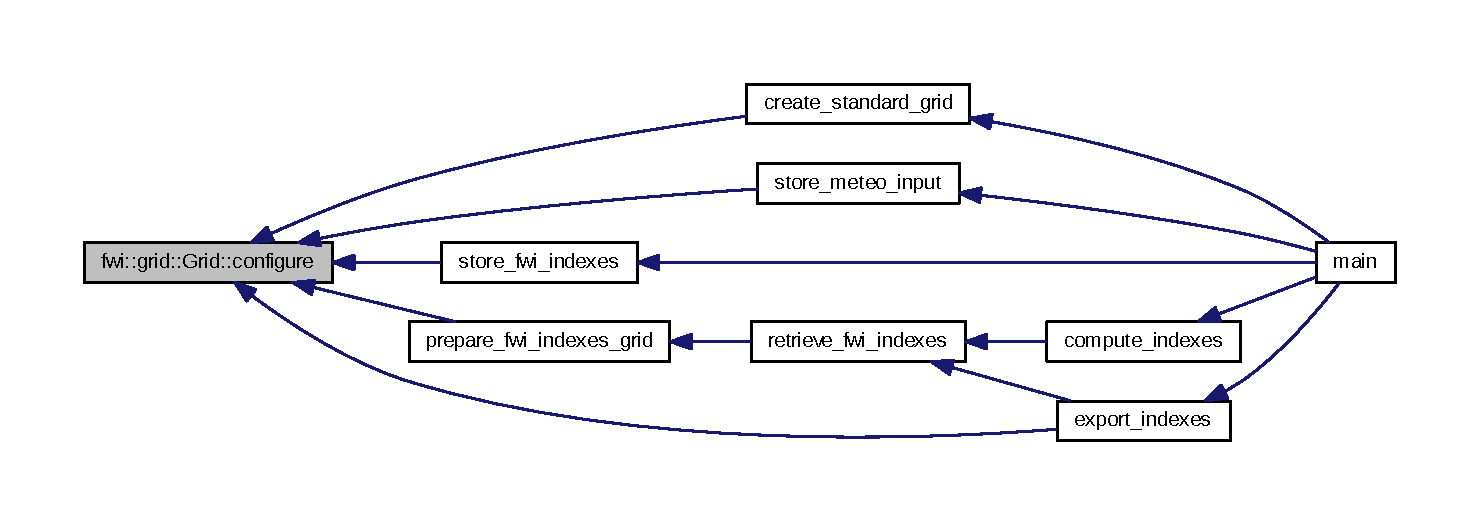
\includegraphics[width=350pt]{classfwi_1_1grid_1_1Grid_abfcac51edc50447a1861ce85d68409cf_icgraph}
\end{center}
\end{figure}


\hypertarget{classfwi_1_1grid_1_1Grid_aaf9b9814c8f513ceba002b75542620c9}{\index{fwi\-::grid\-::\-Grid@{fwi\-::grid\-::\-Grid}!get\-Cols@{get\-Cols}}
\index{get\-Cols@{get\-Cols}!fwi::grid::Grid@{fwi\-::grid\-::\-Grid}}
\subsubsection[{get\-Cols}]{\setlength{\rightskip}{0pt plus 5cm}template$<$typename T $>$ int {\bf fwi\-::grid\-::\-Grid}$<$ T $>$\-::get\-Cols (
\begin{DoxyParamCaption}
{}
\end{DoxyParamCaption}
) const}}\label{classfwi_1_1grid_1_1Grid_aaf9b9814c8f513ceba002b75542620c9}


cols number getter 

\begin{DoxyReturn}{Returns}
grid cols number 
\end{DoxyReturn}


Definition at line 1051 of file Grid.\-h.



Here is the caller graph for this function\-:\nopagebreak
\begin{figure}[H]
\begin{center}
\leavevmode
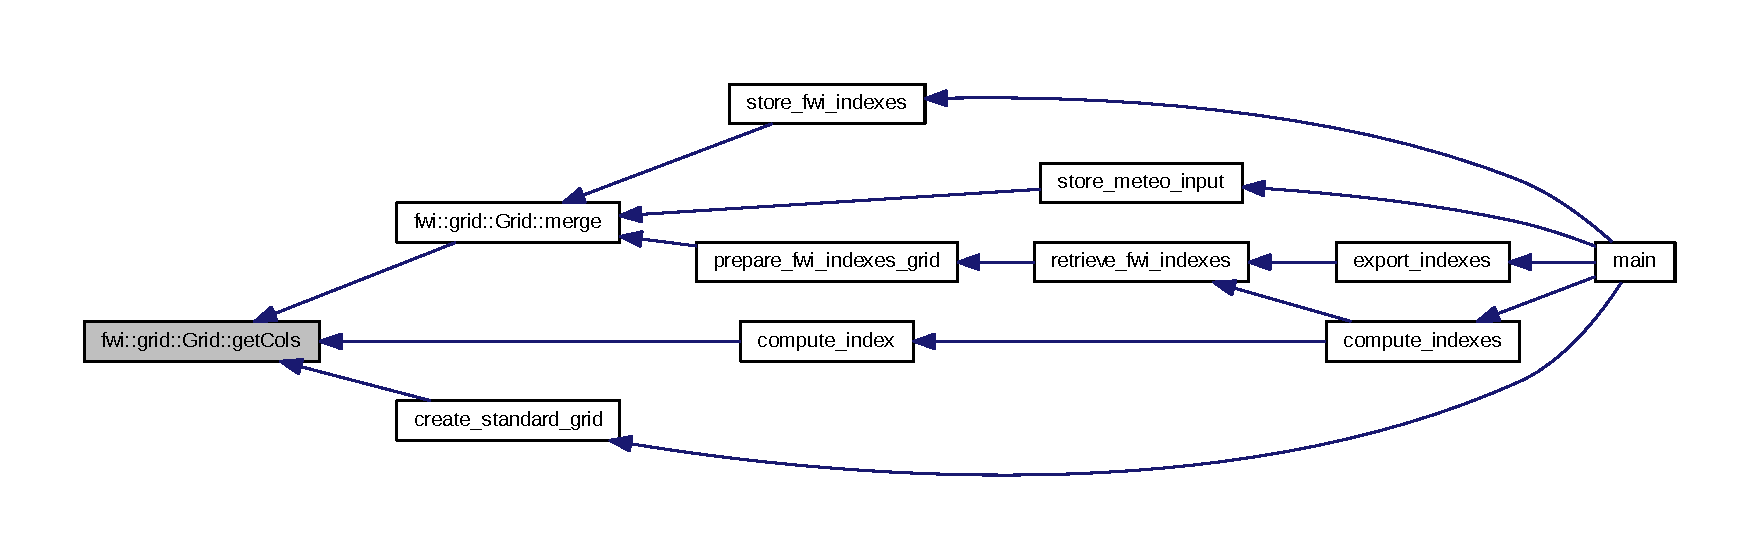
\includegraphics[width=350pt]{classfwi_1_1grid_1_1Grid_aaf9b9814c8f513ceba002b75542620c9_icgraph}
\end{center}
\end{figure}


\hypertarget{classfwi_1_1grid_1_1Grid_a4be1b06ee3d8c6a4eabdd3a402ae3bf9}{\index{fwi\-::grid\-::\-Grid@{fwi\-::grid\-::\-Grid}!get\-Ctl\-Path@{get\-Ctl\-Path}}
\index{get\-Ctl\-Path@{get\-Ctl\-Path}!fwi::grid::Grid@{fwi\-::grid\-::\-Grid}}
\subsubsection[{get\-Ctl\-Path}]{\setlength{\rightskip}{0pt plus 5cm}template$<$typename T $>$ std\-::string {\bf fwi\-::grid\-::\-Grid}$<$ T $>$\-::get\-Ctl\-Path (
\begin{DoxyParamCaption}
{}
\end{DoxyParamCaption}
) const}}\label{classfwi_1_1grid_1_1Grid_a4be1b06ee3d8c6a4eabdd3a402ae3bf9}


grid ctl file path getter 

\begin{DoxyReturn}{Returns}
grid ctl file full path 
\end{DoxyReturn}


Definition at line 1112 of file Grid.\-h.

\hypertarget{classfwi_1_1grid_1_1Grid_a73e900020a90dbad3808d3c91778a3b4}{\index{fwi\-::grid\-::\-Grid@{fwi\-::grid\-::\-Grid}!get\-Data@{get\-Data}}
\index{get\-Data@{get\-Data}!fwi::grid::Grid@{fwi\-::grid\-::\-Grid}}
\subsubsection[{get\-Data}]{\setlength{\rightskip}{0pt plus 5cm}template$<$typename T $>$ {\bf Grid}$<$ T $>$\-::grid\-\_\-t {\bf fwi\-::grid\-::\-Grid}$<$ T $>$\-::get\-Data (
\begin{DoxyParamCaption}
{}
\end{DoxyParamCaption}
)}}\label{classfwi_1_1grid_1_1Grid_a73e900020a90dbad3808d3c91778a3b4}


grid internal data pointer getter 

\begin{DoxyReturn}{Returns}
internal data representation 
\end{DoxyReturn}


Definition at line 1244 of file Grid.\-h.

\hypertarget{classfwi_1_1grid_1_1Grid_ac7c89b5eb43447e86ea0b5b956a8b88d}{\index{fwi\-::grid\-::\-Grid@{fwi\-::grid\-::\-Grid}!get\-Date@{get\-Date}}
\index{get\-Date@{get\-Date}!fwi::grid::Grid@{fwi\-::grid\-::\-Grid}}
\subsubsection[{get\-Date}]{\setlength{\rightskip}{0pt plus 5cm}template$<$typename T $>$ std\-::string {\bf fwi\-::grid\-::\-Grid}$<$ T $>$\-::get\-Date (
\begin{DoxyParamCaption}
{}
\end{DoxyParamCaption}
) const}}\label{classfwi_1_1grid_1_1Grid_ac7c89b5eb43447e86ea0b5b956a8b88d}


date getter 

\begin{DoxyReturn}{Returns}
date current value 
\end{DoxyReturn}


Definition at line 1063 of file Grid.\-h.



Here is the caller graph for this function\-:
\nopagebreak
\begin{figure}[H]
\begin{center}
\leavevmode
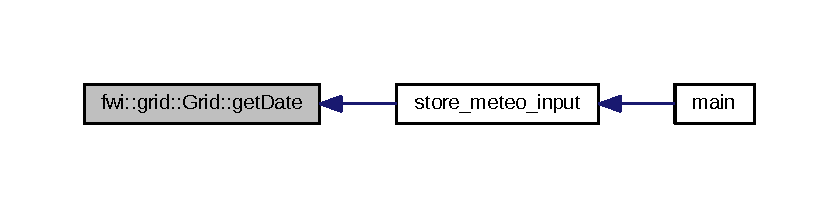
\includegraphics[width=350pt]{classfwi_1_1grid_1_1Grid_ac7c89b5eb43447e86ea0b5b956a8b88d_icgraph}
\end{center}
\end{figure}


\hypertarget{classfwi_1_1grid_1_1Grid_a23e0a0d0fa907ccfbc0881240dc528a2}{\index{fwi\-::grid\-::\-Grid@{fwi\-::grid\-::\-Grid}!get\-Dat\-Path@{get\-Dat\-Path}}
\index{get\-Dat\-Path@{get\-Dat\-Path}!fwi::grid::Grid@{fwi\-::grid\-::\-Grid}}
\subsubsection[{get\-Dat\-Path}]{\setlength{\rightskip}{0pt plus 5cm}template$<$typename T $>$ std\-::string {\bf fwi\-::grid\-::\-Grid}$<$ T $>$\-::get\-Dat\-Path (
\begin{DoxyParamCaption}
{}
\end{DoxyParamCaption}
) const}}\label{classfwi_1_1grid_1_1Grid_a23e0a0d0fa907ccfbc0881240dc528a2}


grid dat file path getter 

\begin{DoxyReturn}{Returns}
grid datfile full path 
\end{DoxyReturn}


Definition at line 1118 of file Grid.\-h.



Here is the caller graph for this function\-:\nopagebreak
\begin{figure}[H]
\begin{center}
\leavevmode
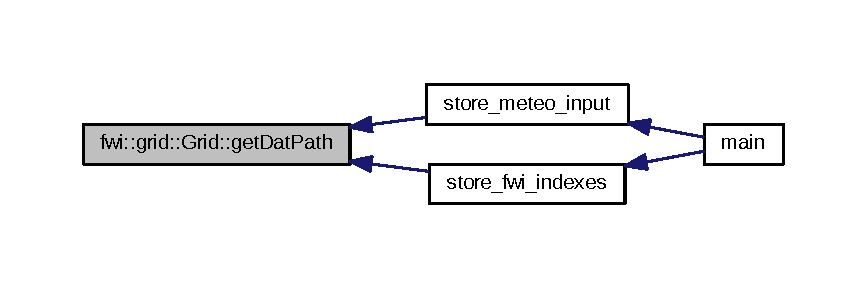
\includegraphics[width=350pt]{classfwi_1_1grid_1_1Grid_a23e0a0d0fa907ccfbc0881240dc528a2_icgraph}
\end{center}
\end{figure}


\hypertarget{classfwi_1_1grid_1_1Grid_abe660314639e862657818d02aad3ff45}{\index{fwi\-::grid\-::\-Grid@{fwi\-::grid\-::\-Grid}!get\-Elements\-Count@{get\-Elements\-Count}}
\index{get\-Elements\-Count@{get\-Elements\-Count}!fwi::grid::Grid@{fwi\-::grid\-::\-Grid}}
\subsubsection[{get\-Elements\-Count}]{\setlength{\rightskip}{0pt plus 5cm}template$<$typename T $>$ int {\bf fwi\-::grid\-::\-Grid}$<$ T $>$\-::get\-Elements\-Count (
\begin{DoxyParamCaption}
{}
\end{DoxyParamCaption}
)}}\label{classfwi_1_1grid_1_1Grid_abe660314639e862657818d02aad3ff45}


gets the element count as rows x cols 

\begin{DoxyReturn}{Returns}
element number only x and y dimensions 
\end{DoxyReturn}


Definition at line 1256 of file Grid.\-h.



Here is the caller graph for this function\-:\nopagebreak
\begin{figure}[H]
\begin{center}
\leavevmode
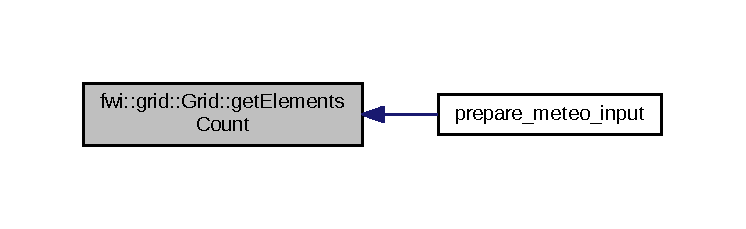
\includegraphics[width=350pt]{classfwi_1_1grid_1_1Grid_abe660314639e862657818d02aad3ff45_icgraph}
\end{center}
\end{figure}


\hypertarget{classfwi_1_1grid_1_1Grid_a2a47f95c96985a5e639285bde471d9a5}{\index{fwi\-::grid\-::\-Grid@{fwi\-::grid\-::\-Grid}!get\-Export\-Ctl\-Path@{get\-Export\-Ctl\-Path}}
\index{get\-Export\-Ctl\-Path@{get\-Export\-Ctl\-Path}!fwi::grid::Grid@{fwi\-::grid\-::\-Grid}}
\subsubsection[{get\-Export\-Ctl\-Path}]{\setlength{\rightskip}{0pt plus 5cm}template$<$typename T $>$ std\-::string {\bf fwi\-::grid\-::\-Grid}$<$ T $>$\-::get\-Export\-Ctl\-Path (
\begin{DoxyParamCaption}
{}
\end{DoxyParamCaption}
) const}}\label{classfwi_1_1grid_1_1Grid_a2a47f95c96985a5e639285bde471d9a5}


grid export ctl file path getter 

\begin{DoxyReturn}{Returns}
grid export ctl file full path 
\end{DoxyReturn}


Definition at line 1124 of file Grid.\-h.



Here is the caller graph for this function\-:\nopagebreak
\begin{figure}[H]
\begin{center}
\leavevmode
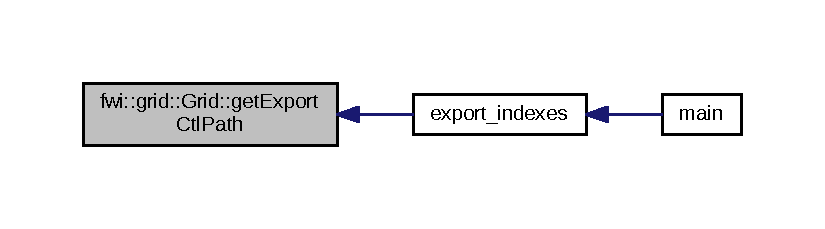
\includegraphics[width=350pt]{classfwi_1_1grid_1_1Grid_a2a47f95c96985a5e639285bde471d9a5_icgraph}
\end{center}
\end{figure}


\hypertarget{classfwi_1_1grid_1_1Grid_a4fdc08766fd405bd37d38a6709c08342}{\index{fwi\-::grid\-::\-Grid@{fwi\-::grid\-::\-Grid}!get\-Export\-Dat\-Path@{get\-Export\-Dat\-Path}}
\index{get\-Export\-Dat\-Path@{get\-Export\-Dat\-Path}!fwi::grid::Grid@{fwi\-::grid\-::\-Grid}}
\subsubsection[{get\-Export\-Dat\-Path}]{\setlength{\rightskip}{0pt plus 5cm}template$<$typename T $>$ std\-::string {\bf fwi\-::grid\-::\-Grid}$<$ T $>$\-::get\-Export\-Dat\-Path (
\begin{DoxyParamCaption}
{}
\end{DoxyParamCaption}
) const}}\label{classfwi_1_1grid_1_1Grid_a4fdc08766fd405bd37d38a6709c08342}


grid export dat file path getter 

\begin{DoxyReturn}{Returns}
grid export datfile full path 
\end{DoxyReturn}


Definition at line 1130 of file Grid.\-h.



Here is the caller graph for this function\-:\nopagebreak
\begin{figure}[H]
\begin{center}
\leavevmode
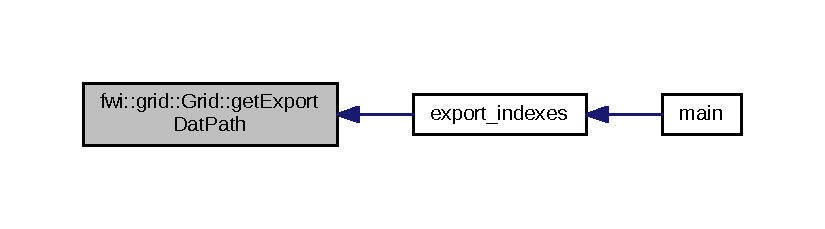
\includegraphics[width=350pt]{classfwi_1_1grid_1_1Grid_a4fdc08766fd405bd37d38a6709c08342_icgraph}
\end{center}
\end{figure}


\hypertarget{classfwi_1_1grid_1_1Grid_a2e891ed3f46840241652cd435ac35a94}{\index{fwi\-::grid\-::\-Grid@{fwi\-::grid\-::\-Grid}!get\-Fields@{get\-Fields}}
\index{get\-Fields@{get\-Fields}!fwi::grid::Grid@{fwi\-::grid\-::\-Grid}}
\subsubsection[{get\-Fields}]{\setlength{\rightskip}{0pt plus 5cm}template$<$typename T $>$ {\bf Grid\-Fields} $\ast$ {\bf fwi\-::grid\-::\-Grid}$<$ T $>$\-::get\-Fields (
\begin{DoxyParamCaption}
{}
\end{DoxyParamCaption}
) const}}\label{classfwi_1_1grid_1_1Grid_a2e891ed3f46840241652cd435ac35a94}


grid fields list getter 

\begin{DoxyReturn}{Returns}
grid fields list 
\end{DoxyReturn}
\begin{DoxySeeAlso}{See also}
\hyperlink{classfwi_1_1grid_1_1GridFields}{Grid\-Fields} 
\end{DoxySeeAlso}


Definition at line 1250 of file Grid.\-h.



Here is the caller graph for this function\-:\nopagebreak
\begin{figure}[H]
\begin{center}
\leavevmode
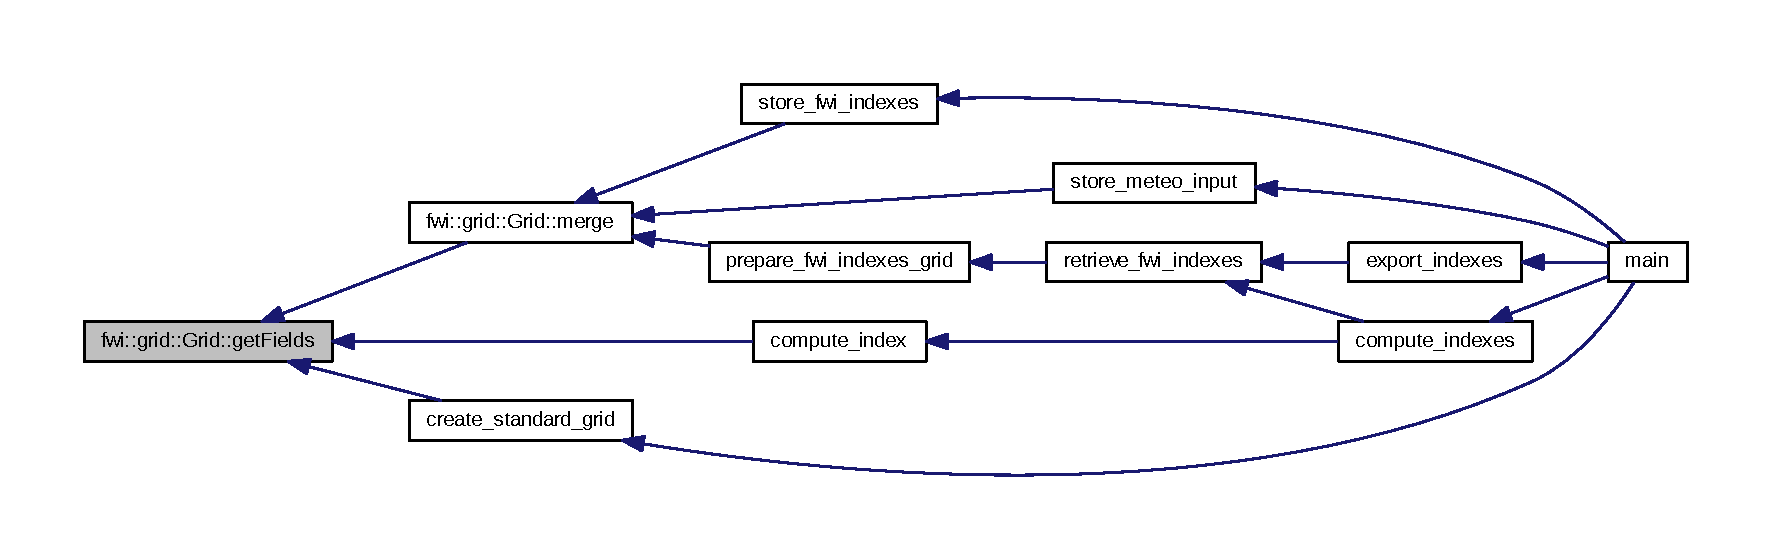
\includegraphics[width=350pt]{classfwi_1_1grid_1_1Grid_a2e891ed3f46840241652cd435ac35a94_icgraph}
\end{center}
\end{figure}


\hypertarget{classfwi_1_1grid_1_1Grid_ac8b97200a77c83bbed7c441fe8414212}{\index{fwi\-::grid\-::\-Grid@{fwi\-::grid\-::\-Grid}!get\-File\-Name\-Date\-Offset@{get\-File\-Name\-Date\-Offset}}
\index{get\-File\-Name\-Date\-Offset@{get\-File\-Name\-Date\-Offset}!fwi::grid::Grid@{fwi\-::grid\-::\-Grid}}
\subsubsection[{get\-File\-Name\-Date\-Offset}]{\setlength{\rightskip}{0pt plus 5cm}template$<$typename T $>$ int {\bf fwi\-::grid\-::\-Grid}$<$ T $>$\-::get\-File\-Name\-Date\-Offset (
\begin{DoxyParamCaption}
{}
\end{DoxyParamCaption}
) const}}\label{classfwi_1_1grid_1_1Grid_ac8b97200a77c83bbed7c441fe8414212}


grid file name date offset getter 

\begin{DoxyReturn}{Returns}
the grid file name date offset in days (+/-\/) 
\end{DoxyReturn}


Definition at line 1172 of file Grid.\-h.

\hypertarget{classfwi_1_1grid_1_1Grid_a51a7b639a01826dc7437d646930f6891}{\index{fwi\-::grid\-::\-Grid@{fwi\-::grid\-::\-Grid}!get\-Grads\-Date@{get\-Grads\-Date}}
\index{get\-Grads\-Date@{get\-Grads\-Date}!fwi::grid::Grid@{fwi\-::grid\-::\-Grid}}
\subsubsection[{get\-Grads\-Date}]{\setlength{\rightskip}{0pt plus 5cm}template$<$typename T $>$ std\-::string {\bf fwi\-::grid\-::\-Grid}$<$ T $>$\-::get\-Grads\-Date (
\begin{DoxyParamCaption}
{}
\end{DoxyParamCaption}
) const}}\label{classfwi_1_1grid_1_1Grid_a51a7b639a01826dc7437d646930f6891}


date in Gr\-A\-D\-S format getter 

\begin{DoxyReturn}{Returns}
date current value 
\end{DoxyReturn}


Definition at line 1084 of file Grid.\-h.

\hypertarget{classfwi_1_1grid_1_1Grid_af6127c6adeb24967516c1d9e0af1a4c6}{\index{fwi\-::grid\-::\-Grid@{fwi\-::grid\-::\-Grid}!get\-I\-O\-Format@{get\-I\-O\-Format}}
\index{get\-I\-O\-Format@{get\-I\-O\-Format}!fwi::grid::Grid@{fwi\-::grid\-::\-Grid}}
\subsubsection[{get\-I\-O\-Format}]{\setlength{\rightskip}{0pt plus 5cm}template$<$typename T $>$ int {\bf fwi\-::grid\-::\-Grid}$<$ T $>$\-::get\-I\-O\-Format (
\begin{DoxyParamCaption}
{}
\end{DoxyParamCaption}
) const}}\label{classfwi_1_1grid_1_1Grid_af6127c6adeb24967516c1d9e0af1a4c6}


grid I/\-O format getter 

\begin{DoxyReturn}{Returns}
grid I/\-O format 
\end{DoxyReturn}
\begin{DoxySeeAlso}{See also}
\hyperlink{fwi__define_8h}{fwi\-\_\-define.\-h} 
\end{DoxySeeAlso}


Definition at line 1178 of file Grid.\-h.

\hypertarget{classfwi_1_1grid_1_1Grid_a7c43b6bb6f6b0d61a6669bd5c7ea8c7a}{\index{fwi\-::grid\-::\-Grid@{fwi\-::grid\-::\-Grid}!get\-Rows@{get\-Rows}}
\index{get\-Rows@{get\-Rows}!fwi::grid::Grid@{fwi\-::grid\-::\-Grid}}
\subsubsection[{get\-Rows}]{\setlength{\rightskip}{0pt plus 5cm}template$<$typename T $>$ int {\bf fwi\-::grid\-::\-Grid}$<$ T $>$\-::get\-Rows (
\begin{DoxyParamCaption}
{}
\end{DoxyParamCaption}
) const}}\label{classfwi_1_1grid_1_1Grid_a7c43b6bb6f6b0d61a6669bd5c7ea8c7a}


rows number getter 

\begin{DoxyReturn}{Returns}
grid rows number 
\end{DoxyReturn}


Definition at line 1045 of file Grid.\-h.



Here is the caller graph for this function\-:\nopagebreak
\begin{figure}[H]
\begin{center}
\leavevmode
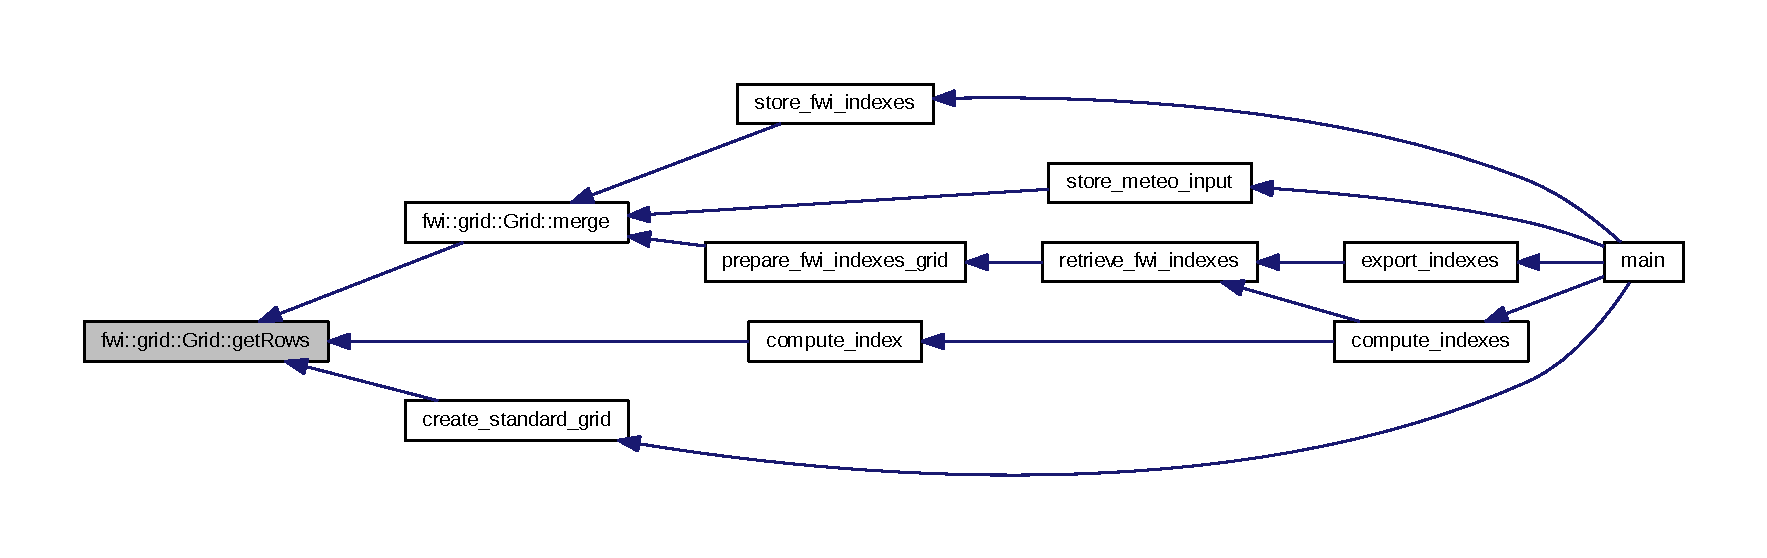
\includegraphics[width=350pt]{classfwi_1_1grid_1_1Grid_a7c43b6bb6f6b0d61a6669bd5c7ea8c7a_icgraph}
\end{center}
\end{figure}


\hypertarget{classfwi_1_1grid_1_1Grid_adf68e16a1b1d07ed1745c57eb6732314}{\index{fwi\-::grid\-::\-Grid@{fwi\-::grid\-::\-Grid}!get\-Slot\-Size@{get\-Slot\-Size}}
\index{get\-Slot\-Size@{get\-Slot\-Size}!fwi::grid::Grid@{fwi\-::grid\-::\-Grid}}
\subsubsection[{get\-Slot\-Size}]{\setlength{\rightskip}{0pt plus 5cm}template$<$typename T $>$ int {\bf fwi\-::grid\-::\-Grid}$<$ T $>$\-::get\-Slot\-Size (
\begin{DoxyParamCaption}
{}
\end{DoxyParamCaption}
) const}}\label{classfwi_1_1grid_1_1Grid_adf68e16a1b1d07ed1745c57eb6732314}


grid slot size getter 

\begin{DoxyReturn}{Returns}
grid slot size 
\end{DoxyReturn}


Definition at line 1238 of file Grid.\-h.



Here is the caller graph for this function\-:\nopagebreak
\begin{figure}[H]
\begin{center}
\leavevmode
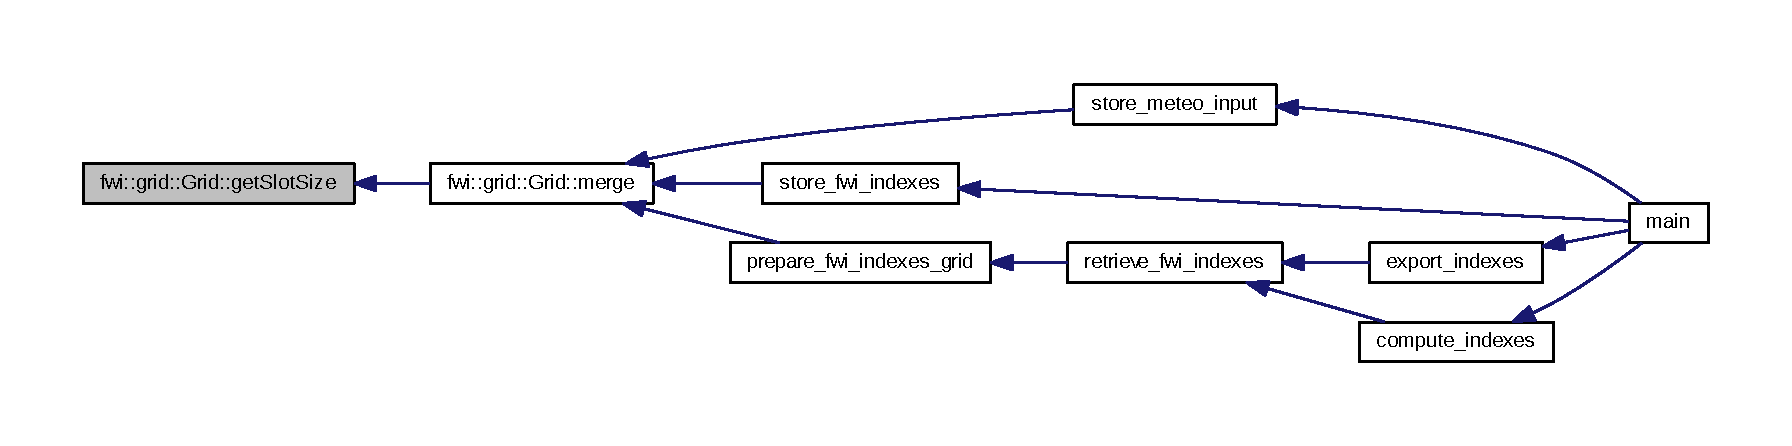
\includegraphics[width=350pt]{classfwi_1_1grid_1_1Grid_adf68e16a1b1d07ed1745c57eb6732314_icgraph}
\end{center}
\end{figure}


\hypertarget{classfwi_1_1grid_1_1Grid_a8aefb75a246d3a618f455d34c7e64f3f}{\index{fwi\-::grid\-::\-Grid@{fwi\-::grid\-::\-Grid}!get\-S\-R\-I\-D@{get\-S\-R\-I\-D}}
\index{get\-S\-R\-I\-D@{get\-S\-R\-I\-D}!fwi::grid::Grid@{fwi\-::grid\-::\-Grid}}
\subsubsection[{get\-S\-R\-I\-D}]{\setlength{\rightskip}{0pt plus 5cm}template$<$typename T $>$ int {\bf fwi\-::grid\-::\-Grid}$<$ T $>$\-::get\-S\-R\-I\-D (
\begin{DoxyParamCaption}
{}
\end{DoxyParamCaption}
) const}}\label{classfwi_1_1grid_1_1Grid_a8aefb75a246d3a618f455d34c7e64f3f}


grid srid getter 

\begin{DoxyReturn}{Returns}
grid srid 
\end{DoxyReturn}


Definition at line 1226 of file Grid.\-h.



Here is the caller graph for this function\-:\nopagebreak
\begin{figure}[H]
\begin{center}
\leavevmode
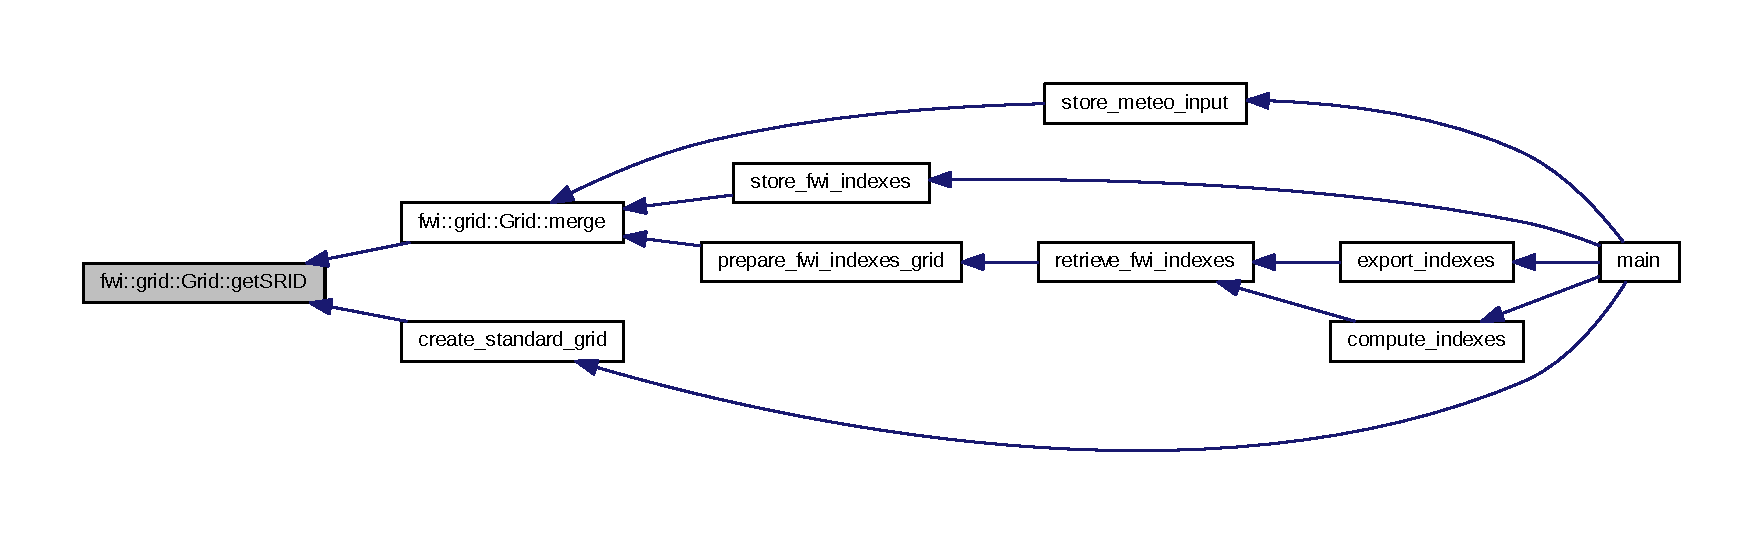
\includegraphics[width=350pt]{classfwi_1_1grid_1_1Grid_a8aefb75a246d3a618f455d34c7e64f3f_icgraph}
\end{center}
\end{figure}


\hypertarget{classfwi_1_1grid_1_1Grid_a869002c87fc7e935b66c40ea712b90e4}{\index{fwi\-::grid\-::\-Grid@{fwi\-::grid\-::\-Grid}!get\-Start\-Time@{get\-Start\-Time}}
\index{get\-Start\-Time@{get\-Start\-Time}!fwi::grid::Grid@{fwi\-::grid\-::\-Grid}}
\subsubsection[{get\-Start\-Time}]{\setlength{\rightskip}{0pt plus 5cm}template$<$typename T $>$ std\-::string {\bf fwi\-::grid\-::\-Grid}$<$ T $>$\-::get\-Start\-Time (
\begin{DoxyParamCaption}
{}
\end{DoxyParamCaption}
) const}}\label{classfwi_1_1grid_1_1Grid_a869002c87fc7e935b66c40ea712b90e4}


grid start time getter 

\begin{DoxyReturn}{Returns}
the grid start time in Gr\-A\-D\-S format 
\end{DoxyReturn}


Definition at line 1160 of file Grid.\-h.

\hypertarget{classfwi_1_1grid_1_1Grid_afc3fafe3429aa908a9af84674dc4c1ee}{\index{fwi\-::grid\-::\-Grid@{fwi\-::grid\-::\-Grid}!get\-Table@{get\-Table}}
\index{get\-Table@{get\-Table}!fwi::grid::Grid@{fwi\-::grid\-::\-Grid}}
\subsubsection[{get\-Table}]{\setlength{\rightskip}{0pt plus 5cm}template$<$typename T $>$ std\-::string {\bf fwi\-::grid\-::\-Grid}$<$ T $>$\-::get\-Table (
\begin{DoxyParamCaption}
{}
\end{DoxyParamCaption}
) const}}\label{classfwi_1_1grid_1_1Grid_afc3fafe3429aa908a9af84674dc4c1ee}


grid database table name getter 

\begin{DoxyReturn}{Returns}
table name 
\end{DoxyReturn}


Definition at line 1057 of file Grid.\-h.



Here is the caller graph for this function\-:\nopagebreak
\begin{figure}[H]
\begin{center}
\leavevmode
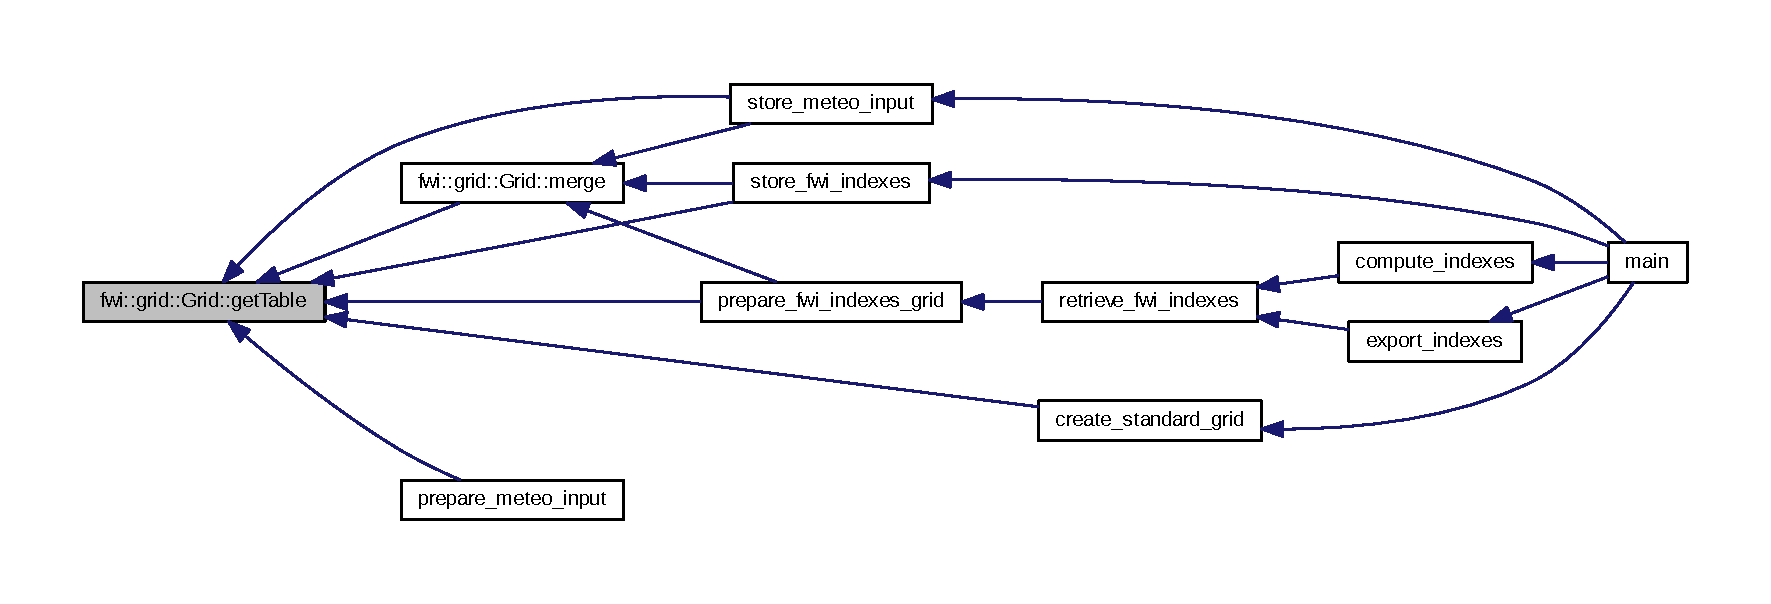
\includegraphics[width=350pt]{classfwi_1_1grid_1_1Grid_afc3fafe3429aa908a9af84674dc4c1ee_icgraph}
\end{center}
\end{figure}


\hypertarget{classfwi_1_1grid_1_1Grid_ae9043ae6499a47872c6161516b721e21}{\index{fwi\-::grid\-::\-Grid@{fwi\-::grid\-::\-Grid}!get\-Time\-Band@{get\-Time\-Band}}
\index{get\-Time\-Band@{get\-Time\-Band}!fwi::grid::Grid@{fwi\-::grid\-::\-Grid}}
\subsubsection[{get\-Time\-Band}]{\setlength{\rightskip}{0pt plus 5cm}template$<$typename T $>$ int {\bf fwi\-::grid\-::\-Grid}$<$ T $>$\-::get\-Time\-Band (
\begin{DoxyParamCaption}
{}
\end{DoxyParamCaption}
) const}}\label{classfwi_1_1grid_1_1Grid_ae9043ae6499a47872c6161516b721e21}


grid time band 

\begin{DoxyReturn}{Returns}
the grid time band 
\end{DoxyReturn}


Definition at line 1148 of file Grid.\-h.

\hypertarget{classfwi_1_1grid_1_1Grid_ac6f053b3983bf2f651a1a523b8591be4}{\index{fwi\-::grid\-::\-Grid@{fwi\-::grid\-::\-Grid}!get\-Time\-Bands\-Number@{get\-Time\-Bands\-Number}}
\index{get\-Time\-Bands\-Number@{get\-Time\-Bands\-Number}!fwi::grid::Grid@{fwi\-::grid\-::\-Grid}}
\subsubsection[{get\-Time\-Bands\-Number}]{\setlength{\rightskip}{0pt plus 5cm}template$<$typename T $>$ int {\bf fwi\-::grid\-::\-Grid}$<$ T $>$\-::get\-Time\-Bands\-Number (
\begin{DoxyParamCaption}
{}
\end{DoxyParamCaption}
) const}}\label{classfwi_1_1grid_1_1Grid_ac6f053b3983bf2f651a1a523b8591be4}


grid time bands number 

\begin{DoxyReturn}{Returns}
the grid time bands number 
\end{DoxyReturn}


Definition at line 1154 of file Grid.\-h.

\hypertarget{classfwi_1_1grid_1_1Grid_aa6a35277617cbae5fe3db3f9ae28558d}{\index{fwi\-::grid\-::\-Grid@{fwi\-::grid\-::\-Grid}!get\-Time\-Increment@{get\-Time\-Increment}}
\index{get\-Time\-Increment@{get\-Time\-Increment}!fwi::grid::Grid@{fwi\-::grid\-::\-Grid}}
\subsubsection[{get\-Time\-Increment}]{\setlength{\rightskip}{0pt plus 5cm}template$<$typename T $>$ std\-::string {\bf fwi\-::grid\-::\-Grid}$<$ T $>$\-::get\-Time\-Increment (
\begin{DoxyParamCaption}
{}
\end{DoxyParamCaption}
) const}}\label{classfwi_1_1grid_1_1Grid_aa6a35277617cbae5fe3db3f9ae28558d}


grid time increment getter 

\begin{DoxyReturn}{Returns}
the grid time increment in Gr\-A\-D\-S format 
\end{DoxyReturn}


Definition at line 1166 of file Grid.\-h.

\hypertarget{classfwi_1_1grid_1_1Grid_a7e9e12dc12588d1834c261b610cac319}{\index{fwi\-::grid\-::\-Grid@{fwi\-::grid\-::\-Grid}!get\-Title@{get\-Title}}
\index{get\-Title@{get\-Title}!fwi::grid::Grid@{fwi\-::grid\-::\-Grid}}
\subsubsection[{get\-Title}]{\setlength{\rightskip}{0pt plus 5cm}template$<$typename T $>$ std\-::string {\bf fwi\-::grid\-::\-Grid}$<$ T $>$\-::get\-Title (
\begin{DoxyParamCaption}
{}
\end{DoxyParamCaption}
) const}}\label{classfwi_1_1grid_1_1Grid_a7e9e12dc12588d1834c261b610cac319}


grid title getter 

\begin{DoxyReturn}{Returns}
the grid title as in grib files 
\end{DoxyReturn}


Definition at line 1136 of file Grid.\-h.

\hypertarget{classfwi_1_1grid_1_1Grid_aa140c12f1edfb152b7e859488969cf3e}{\index{fwi\-::grid\-::\-Grid@{fwi\-::grid\-::\-Grid}!get\-Total\-Elements\-Count@{get\-Total\-Elements\-Count}}
\index{get\-Total\-Elements\-Count@{get\-Total\-Elements\-Count}!fwi::grid::Grid@{fwi\-::grid\-::\-Grid}}
\subsubsection[{get\-Total\-Elements\-Count}]{\setlength{\rightskip}{0pt plus 5cm}template$<$typename T $>$ int {\bf fwi\-::grid\-::\-Grid}$<$ T $>$\-::get\-Total\-Elements\-Count (
\begin{DoxyParamCaption}
{}
\end{DoxyParamCaption}
)}}\label{classfwi_1_1grid_1_1Grid_aa140c12f1edfb152b7e859488969cf3e}


gets the total element count as rows x cols x var\-Num 

\begin{DoxyReturn}{Returns}
element total number 
\end{DoxyReturn}


Definition at line 1262 of file Grid.\-h.

\hypertarget{classfwi_1_1grid_1_1Grid_a2deb54df5fc5e90b3b5b061a516c2a92}{\index{fwi\-::grid\-::\-Grid@{fwi\-::grid\-::\-Grid}!get\-Type@{get\-Type}}
\index{get\-Type@{get\-Type}!fwi::grid::Grid@{fwi\-::grid\-::\-Grid}}
\subsubsection[{get\-Type}]{\setlength{\rightskip}{0pt plus 5cm}template$<$typename T $>$ int {\bf fwi\-::grid\-::\-Grid}$<$ T $>$\-::get\-Type (
\begin{DoxyParamCaption}
{}
\end{DoxyParamCaption}
) const}}\label{classfwi_1_1grid_1_1Grid_a2deb54df5fc5e90b3b5b061a516c2a92}


grid type getter 

\begin{DoxyReturn}{Returns}
grid type 
\end{DoxyReturn}
\begin{DoxySeeAlso}{See also}
\hyperlink{fwi__define_8h}{fwi\-\_\-define.\-h} 
\end{DoxySeeAlso}


Definition at line 1142 of file Grid.\-h.



Here is the caller graph for this function\-:\nopagebreak
\begin{figure}[H]
\begin{center}
\leavevmode
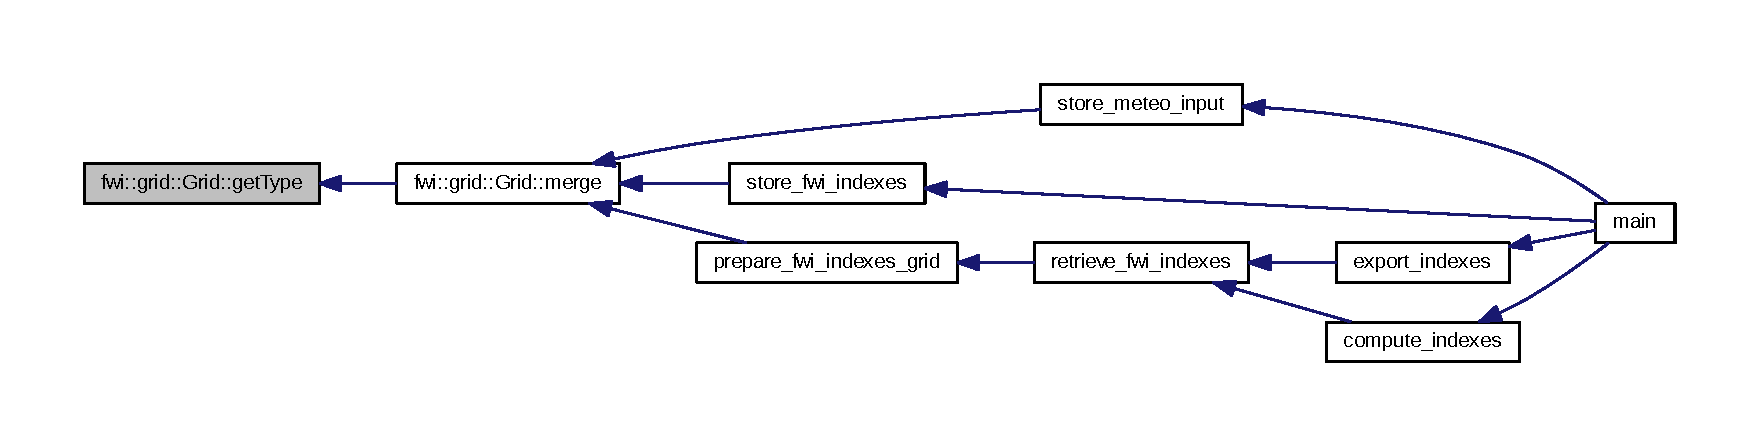
\includegraphics[width=350pt]{classfwi_1_1grid_1_1Grid_a2deb54df5fc5e90b3b5b061a516c2a92_icgraph}
\end{center}
\end{figure}


\hypertarget{classfwi_1_1grid_1_1Grid_a8d18ce74846ea7432f034a30ef879b59}{\index{fwi\-::grid\-::\-Grid@{fwi\-::grid\-::\-Grid}!get\-Undef\-Value@{get\-Undef\-Value}}
\index{get\-Undef\-Value@{get\-Undef\-Value}!fwi::grid::Grid@{fwi\-::grid\-::\-Grid}}
\subsubsection[{get\-Undef\-Value}]{\setlength{\rightskip}{0pt plus 5cm}template$<$typename T $>$ float {\bf fwi\-::grid\-::\-Grid}$<$ T $>$\-::get\-Undef\-Value (
\begin{DoxyParamCaption}
{}
\end{DoxyParamCaption}
) const}}\label{classfwi_1_1grid_1_1Grid_a8d18ce74846ea7432f034a30ef879b59}


grid undefindined value getter 

\begin{DoxyReturn}{Returns}
grid undefined value 
\end{DoxyReturn}


Definition at line 1232 of file Grid.\-h.



Here is the caller graph for this function\-:\nopagebreak
\begin{figure}[H]
\begin{center}
\leavevmode
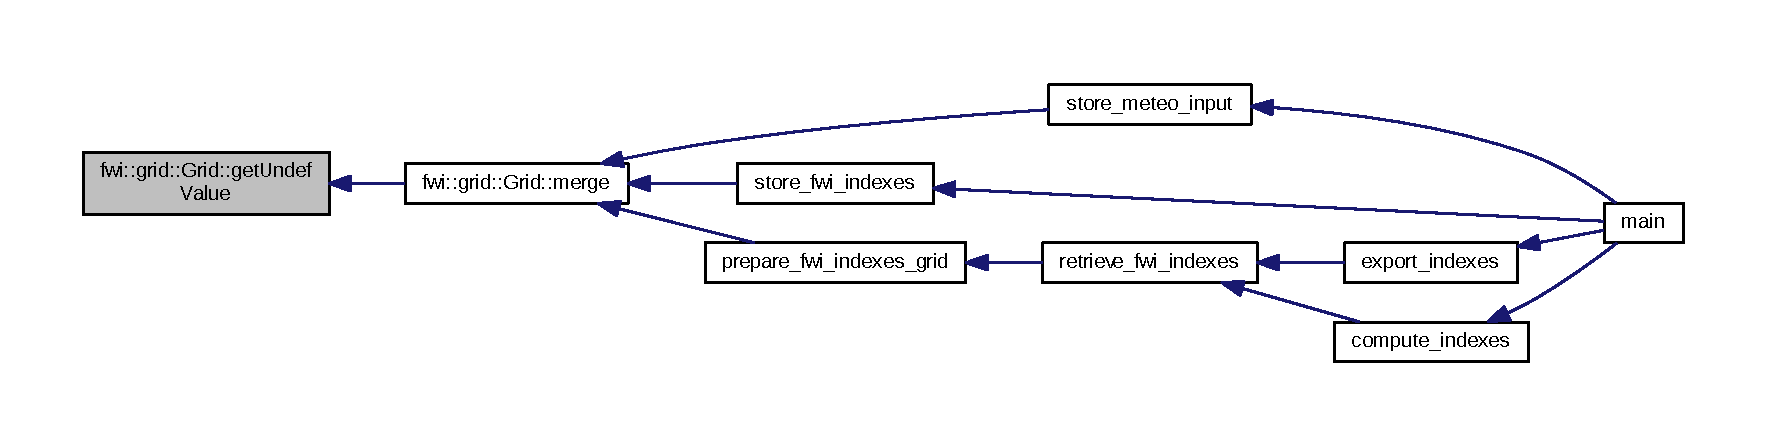
\includegraphics[width=350pt]{classfwi_1_1grid_1_1Grid_a8d18ce74846ea7432f034a30ef879b59_icgraph}
\end{center}
\end{figure}


\hypertarget{classfwi_1_1grid_1_1Grid_ad9e9ac91e9c338606e1199ffa89fc6bb}{\index{fwi\-::grid\-::\-Grid@{fwi\-::grid\-::\-Grid}!get\-Var\-Num@{get\-Var\-Num}}
\index{get\-Var\-Num@{get\-Var\-Num}!fwi::grid::Grid@{fwi\-::grid\-::\-Grid}}
\subsubsection[{get\-Var\-Num}]{\setlength{\rightskip}{0pt plus 5cm}template$<$typename T $>$ int {\bf fwi\-::grid\-::\-Grid}$<$ T $>$\-::get\-Var\-Num (
\begin{DoxyParamCaption}
{}
\end{DoxyParamCaption}
) const}}\label{classfwi_1_1grid_1_1Grid_ad9e9ac91e9c338606e1199ffa89fc6bb}


variables number getter 

\begin{DoxyReturn}{Returns}
variables number 
\end{DoxyReturn}


Definition at line 1220 of file Grid.\-h.



Here is the caller graph for this function\-:\nopagebreak
\begin{figure}[H]
\begin{center}
\leavevmode
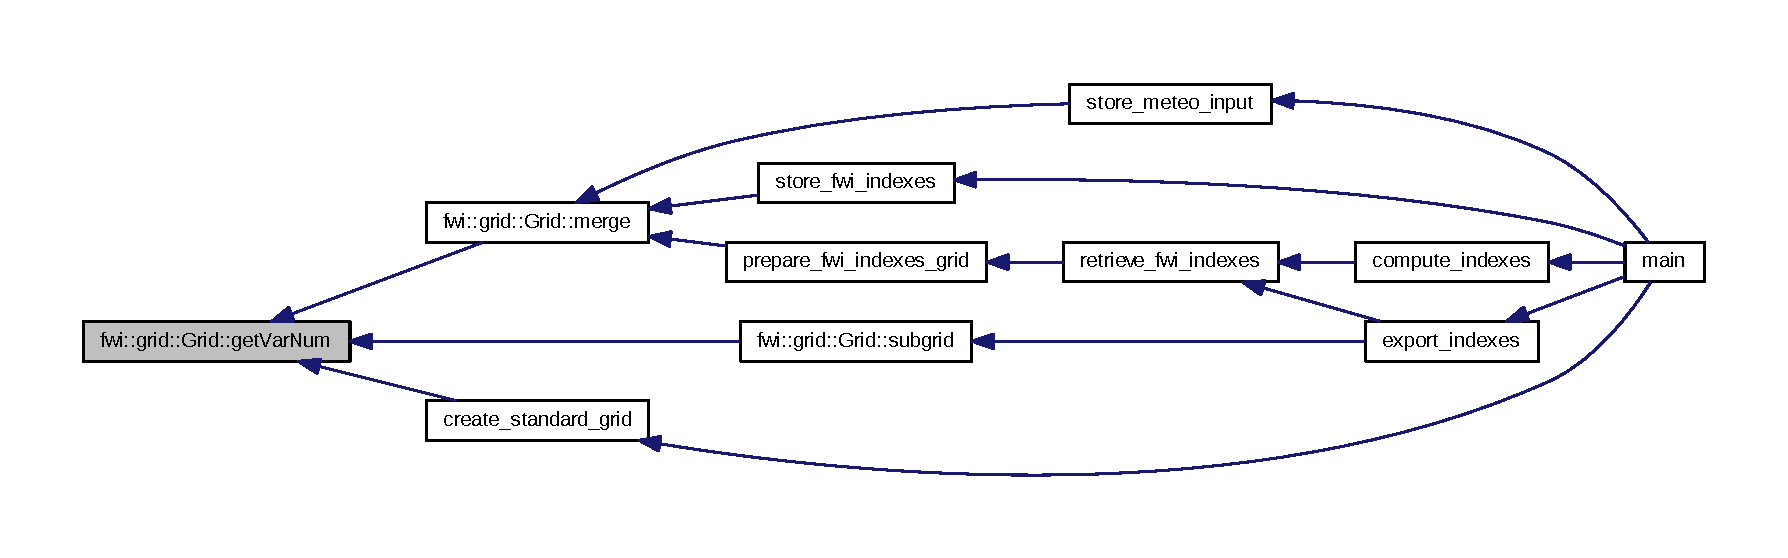
\includegraphics[width=350pt]{classfwi_1_1grid_1_1Grid_ad9e9ac91e9c338606e1199ffa89fc6bb_icgraph}
\end{center}
\end{figure}


\hypertarget{classfwi_1_1grid_1_1Grid_a60d11b4f03f3ed4ef4349d25897486d7}{\index{fwi\-::grid\-::\-Grid@{fwi\-::grid\-::\-Grid}!get\-X\-Dir@{get\-X\-Dir}}
\index{get\-X\-Dir@{get\-X\-Dir}!fwi::grid::Grid@{fwi\-::grid\-::\-Grid}}
\subsubsection[{get\-X\-Dir}]{\setlength{\rightskip}{0pt plus 5cm}template$<$typename T $>$ C\-O\-O\-R\-D\-I\-N\-A\-T\-E\-\_\-\-D\-I\-R\-E\-C\-T\-I\-O\-N {\bf fwi\-::grid\-::\-Grid}$<$ T $>$\-::get\-X\-Dir (
\begin{DoxyParamCaption}
{}
\end{DoxyParamCaption}
) const}}\label{classfwi_1_1grid_1_1Grid_a60d11b4f03f3ed4ef4349d25897486d7}


x\-Dir getter 

\begin{DoxyReturn}{Returns}
current value for x\-Dir 
\end{DoxyReturn}


Definition at line 1208 of file Grid.\-h.

\hypertarget{classfwi_1_1grid_1_1Grid_ae2feb145847b2504ca2474a9e3e33945}{\index{fwi\-::grid\-::\-Grid@{fwi\-::grid\-::\-Grid}!get\-X\-Start@{get\-X\-Start}}
\index{get\-X\-Start@{get\-X\-Start}!fwi::grid::Grid@{fwi\-::grid\-::\-Grid}}
\subsubsection[{get\-X\-Start}]{\setlength{\rightskip}{0pt plus 5cm}template$<$typename T $>$ float {\bf fwi\-::grid\-::\-Grid}$<$ T $>$\-::get\-X\-Start (
\begin{DoxyParamCaption}
{}
\end{DoxyParamCaption}
) const}}\label{classfwi_1_1grid_1_1Grid_ae2feb145847b2504ca2474a9e3e33945}


grid start x coordinate getter 

\begin{DoxyReturn}{Returns}
grid start x coordinate 
\end{DoxyReturn}


Definition at line 1184 of file Grid.\-h.



Here is the caller graph for this function\-:\nopagebreak
\begin{figure}[H]
\begin{center}
\leavevmode
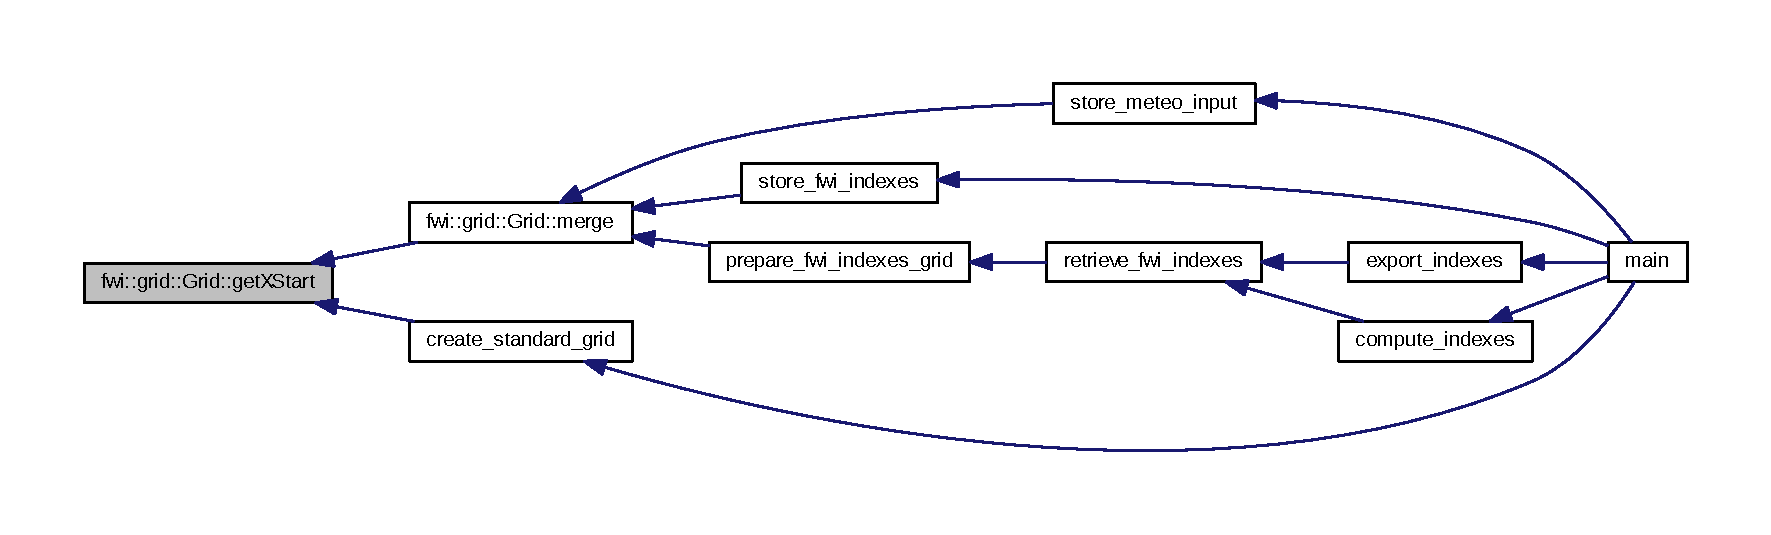
\includegraphics[width=350pt]{classfwi_1_1grid_1_1Grid_ae2feb145847b2504ca2474a9e3e33945_icgraph}
\end{center}
\end{figure}


\hypertarget{classfwi_1_1grid_1_1Grid_ac2986f115fadf2ef16cf0b9e61114baf}{\index{fwi\-::grid\-::\-Grid@{fwi\-::grid\-::\-Grid}!get\-X\-Step@{get\-X\-Step}}
\index{get\-X\-Step@{get\-X\-Step}!fwi::grid::Grid@{fwi\-::grid\-::\-Grid}}
\subsubsection[{get\-X\-Step}]{\setlength{\rightskip}{0pt plus 5cm}template$<$typename T $>$ float {\bf fwi\-::grid\-::\-Grid}$<$ T $>$\-::get\-X\-Step (
\begin{DoxyParamCaption}
{}
\end{DoxyParamCaption}
) const}}\label{classfwi_1_1grid_1_1Grid_ac2986f115fadf2ef16cf0b9e61114baf}


grid step in x direction getter 

\begin{DoxyReturn}{Returns}
grid step in x direction 
\end{DoxyReturn}


Definition at line 1190 of file Grid.\-h.



Here is the caller graph for this function\-:\nopagebreak
\begin{figure}[H]
\begin{center}
\leavevmode
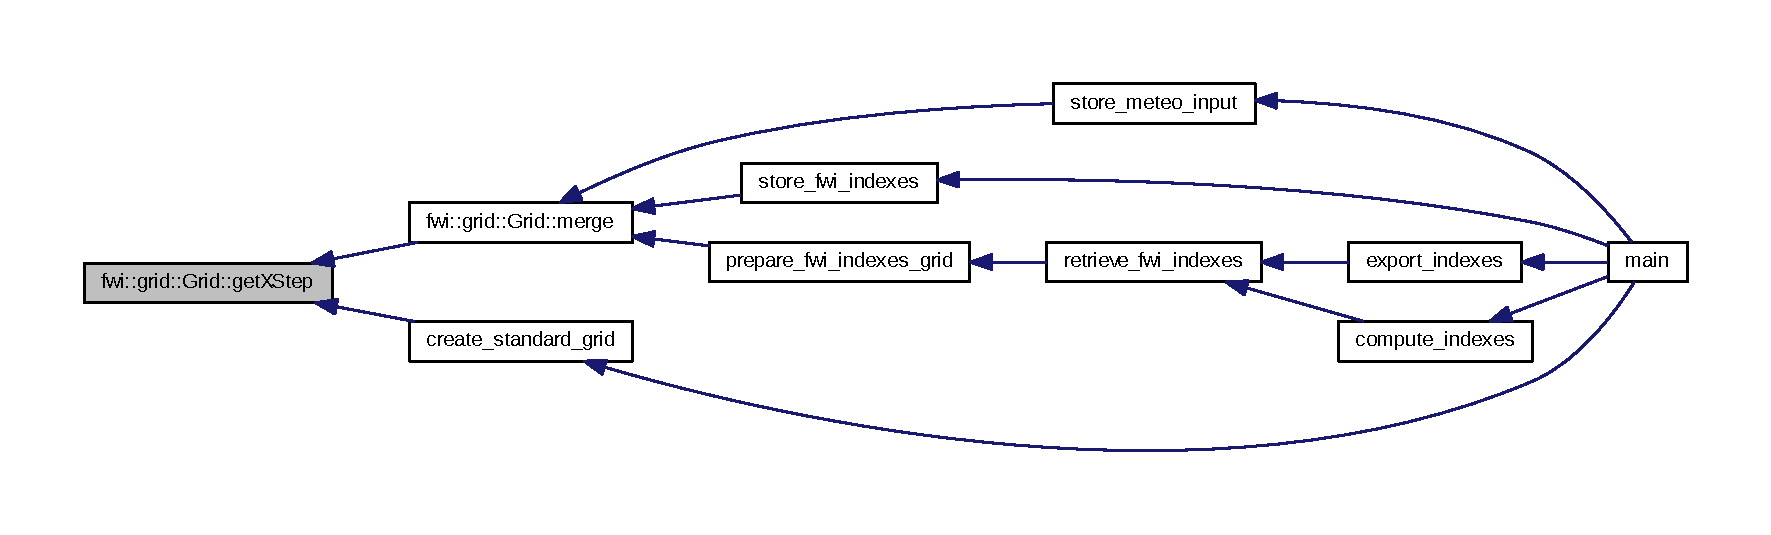
\includegraphics[width=350pt]{classfwi_1_1grid_1_1Grid_ac2986f115fadf2ef16cf0b9e61114baf_icgraph}
\end{center}
\end{figure}


\hypertarget{classfwi_1_1grid_1_1Grid_ac8761c50efb6f2af694727b9b12d9f0e}{\index{fwi\-::grid\-::\-Grid@{fwi\-::grid\-::\-Grid}!get\-Y\-Dir@{get\-Y\-Dir}}
\index{get\-Y\-Dir@{get\-Y\-Dir}!fwi::grid::Grid@{fwi\-::grid\-::\-Grid}}
\subsubsection[{get\-Y\-Dir}]{\setlength{\rightskip}{0pt plus 5cm}template$<$typename T $>$ C\-O\-O\-R\-D\-I\-N\-A\-T\-E\-\_\-\-D\-I\-R\-E\-C\-T\-I\-O\-N {\bf fwi\-::grid\-::\-Grid}$<$ T $>$\-::get\-Y\-Dir (
\begin{DoxyParamCaption}
{}
\end{DoxyParamCaption}
) const}}\label{classfwi_1_1grid_1_1Grid_ac8761c50efb6f2af694727b9b12d9f0e}


y\-Dir getter 

\begin{DoxyReturn}{Returns}
current value for y\-Dir 
\end{DoxyReturn}


Definition at line 1214 of file Grid.\-h.

\hypertarget{classfwi_1_1grid_1_1Grid_a5e41f9d7886b318044b1de323d075d54}{\index{fwi\-::grid\-::\-Grid@{fwi\-::grid\-::\-Grid}!get\-Y\-Start@{get\-Y\-Start}}
\index{get\-Y\-Start@{get\-Y\-Start}!fwi::grid::Grid@{fwi\-::grid\-::\-Grid}}
\subsubsection[{get\-Y\-Start}]{\setlength{\rightskip}{0pt plus 5cm}template$<$typename T $>$ float {\bf fwi\-::grid\-::\-Grid}$<$ T $>$\-::get\-Y\-Start (
\begin{DoxyParamCaption}
{}
\end{DoxyParamCaption}
) const}}\label{classfwi_1_1grid_1_1Grid_a5e41f9d7886b318044b1de323d075d54}


grid start y coordinate getter 

\begin{DoxyReturn}{Returns}
grid start y coordinate 
\end{DoxyReturn}


Definition at line 1196 of file Grid.\-h.



Here is the caller graph for this function\-:\nopagebreak
\begin{figure}[H]
\begin{center}
\leavevmode
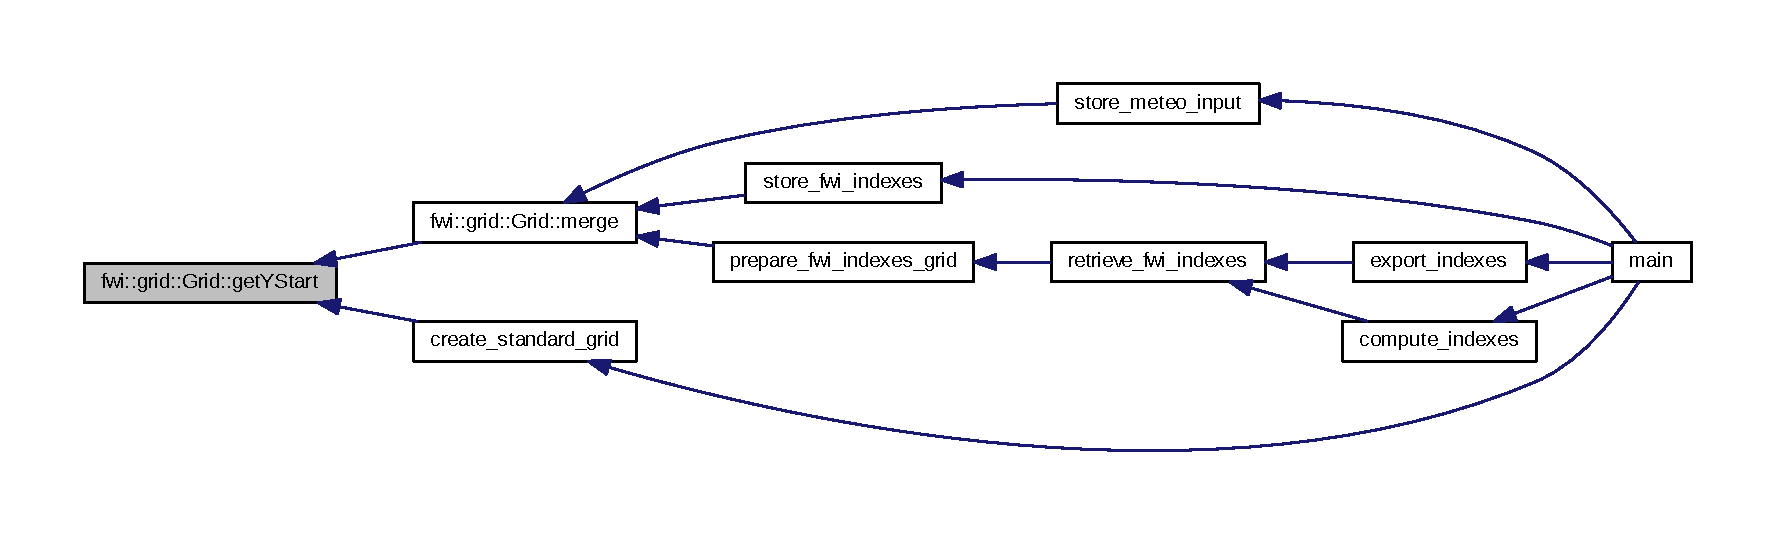
\includegraphics[width=350pt]{classfwi_1_1grid_1_1Grid_a5e41f9d7886b318044b1de323d075d54_icgraph}
\end{center}
\end{figure}


\hypertarget{classfwi_1_1grid_1_1Grid_aae81a8e8fddf00750337a86bc6940337}{\index{fwi\-::grid\-::\-Grid@{fwi\-::grid\-::\-Grid}!get\-Y\-Step@{get\-Y\-Step}}
\index{get\-Y\-Step@{get\-Y\-Step}!fwi::grid::Grid@{fwi\-::grid\-::\-Grid}}
\subsubsection[{get\-Y\-Step}]{\setlength{\rightskip}{0pt plus 5cm}template$<$typename T $>$ float {\bf fwi\-::grid\-::\-Grid}$<$ T $>$\-::get\-Y\-Step (
\begin{DoxyParamCaption}
{}
\end{DoxyParamCaption}
) const}}\label{classfwi_1_1grid_1_1Grid_aae81a8e8fddf00750337a86bc6940337}


grid step in y direction getter 

\begin{DoxyReturn}{Returns}
grid step in y direction 
\end{DoxyReturn}


Definition at line 1202 of file Grid.\-h.



Here is the caller graph for this function\-:\nopagebreak
\begin{figure}[H]
\begin{center}
\leavevmode
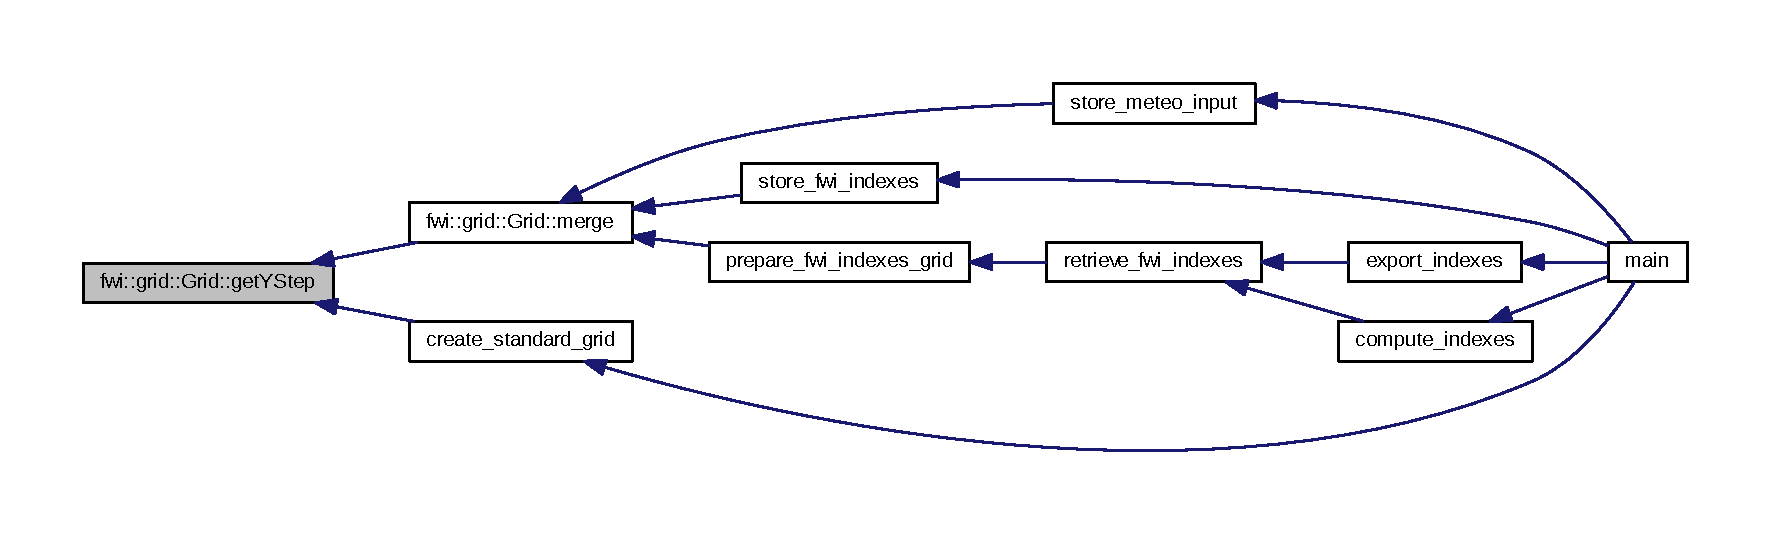
\includegraphics[width=350pt]{classfwi_1_1grid_1_1Grid_aae81a8e8fddf00750337a86bc6940337_icgraph}
\end{center}
\end{figure}


\hypertarget{classfwi_1_1grid_1_1Grid_a65a165655dd630f5f1b7c52b4e261059}{\index{fwi\-::grid\-::\-Grid@{fwi\-::grid\-::\-Grid}!insert@{insert}}
\index{insert@{insert}!fwi::grid::Grid@{fwi\-::grid\-::\-Grid}}
\subsubsection[{insert}]{\setlength{\rightskip}{0pt plus 5cm}template$<$typename T $>$ bool {\bf fwi\-::grid\-::\-Grid}$<$ T $>$\-::insert (
\begin{DoxyParamCaption}
\item[{P\-Gconn $\ast$}]{conn}
\end{DoxyParamCaption}
)}}\label{classfwi_1_1grid_1_1Grid_a65a165655dd630f5f1b7c52b4e261059}


insert grid in database 


\begin{DoxyParams}{Parameters}
{\em conn} & postgresql connection \\
\hline
\end{DoxyParams}
\begin{DoxyReturn}{Returns}
true on success else false 
\end{DoxyReturn}
\begin{DoxySeeAlso}{See also}
postgresql documentation at \href{http://www.postgresql.org/}{\tt http\-://www.\-postgresql.\-org/} 
\end{DoxySeeAlso}


Definition at line 2213 of file Grid.\-h.

\hypertarget{classfwi_1_1grid_1_1Grid_a254a6c5a649b7d3a109f67811ef5f356}{\index{fwi\-::grid\-::\-Grid@{fwi\-::grid\-::\-Grid}!merge@{merge}}
\index{merge@{merge}!fwi::grid::Grid@{fwi\-::grid\-::\-Grid}}
\subsubsection[{merge}]{\setlength{\rightskip}{0pt plus 5cm}template$<$typename T $>$ bool {\bf fwi\-::grid\-::\-Grid}$<$ T $>$\-::merge (
\begin{DoxyParamCaption}
\item[{{\bf Grid}$<$ T $>$ \&}]{other}
\end{DoxyParamCaption}
)}}\label{classfwi_1_1grid_1_1Grid_a254a6c5a649b7d3a109f67811ef5f356}


merges {\itshape other} whith {\bfseries this} 


\begin{DoxyParams}{Parameters}
{\em other} & second grid \begin{DoxyVerb}     merge can be done only if
     rows     == other.getRows()     && cols       == other.getCols()       and
     xStart   == other.getXStart()   && yStart     == other.getYStart()     and
     xStep    == other.getXStep()    && yStep      == other.getYStep()      and
     type     == other.getType()     && srid       == other.getSRID()       and
     slotSize == other.getSlotSize() && undefValue == other.getUndefValue() and
     table    == other.getTable()
\end{DoxyVerb}
\\
\hline
\end{DoxyParams}
\begin{DoxyReturn}{Returns}
true on success else false 
\end{DoxyReturn}


Definition at line 1652 of file Grid.\-h.



Here is the call graph for this function\-:\nopagebreak
\begin{figure}[H]
\begin{center}
\leavevmode
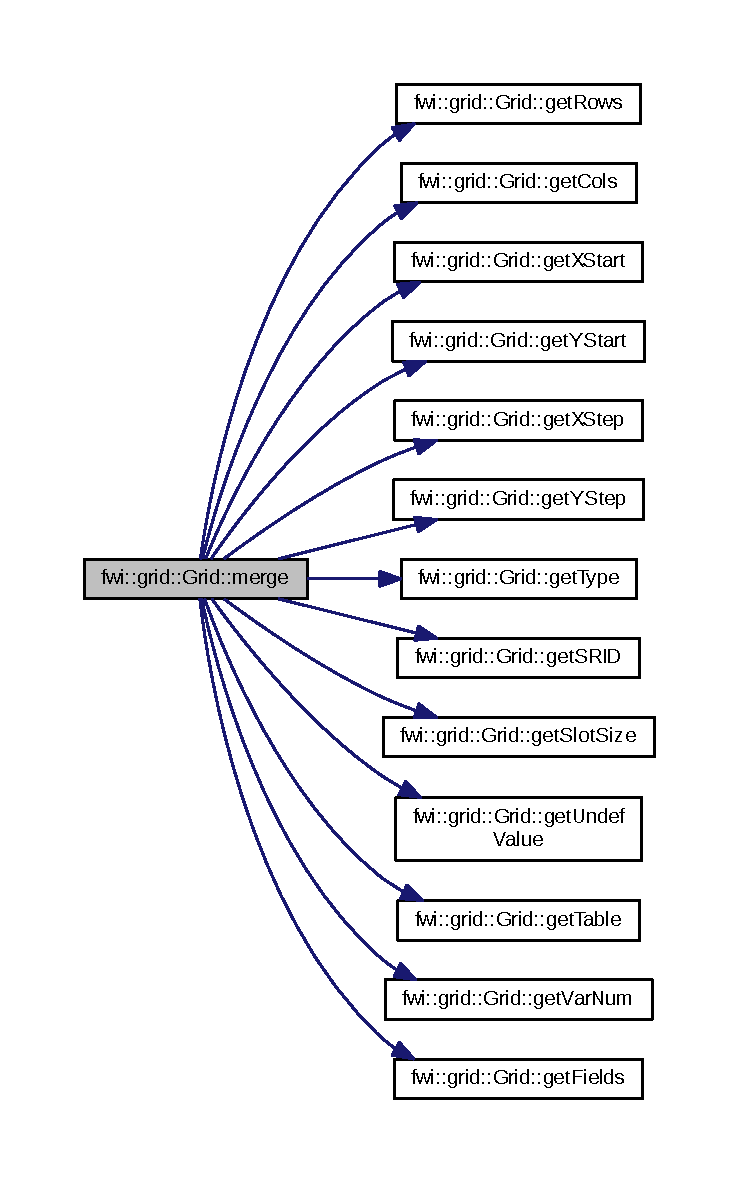
\includegraphics[height=550pt]{classfwi_1_1grid_1_1Grid_a254a6c5a649b7d3a109f67811ef5f356_cgraph}
\end{center}
\end{figure}




Here is the caller graph for this function\-:\nopagebreak
\begin{figure}[H]
\begin{center}
\leavevmode
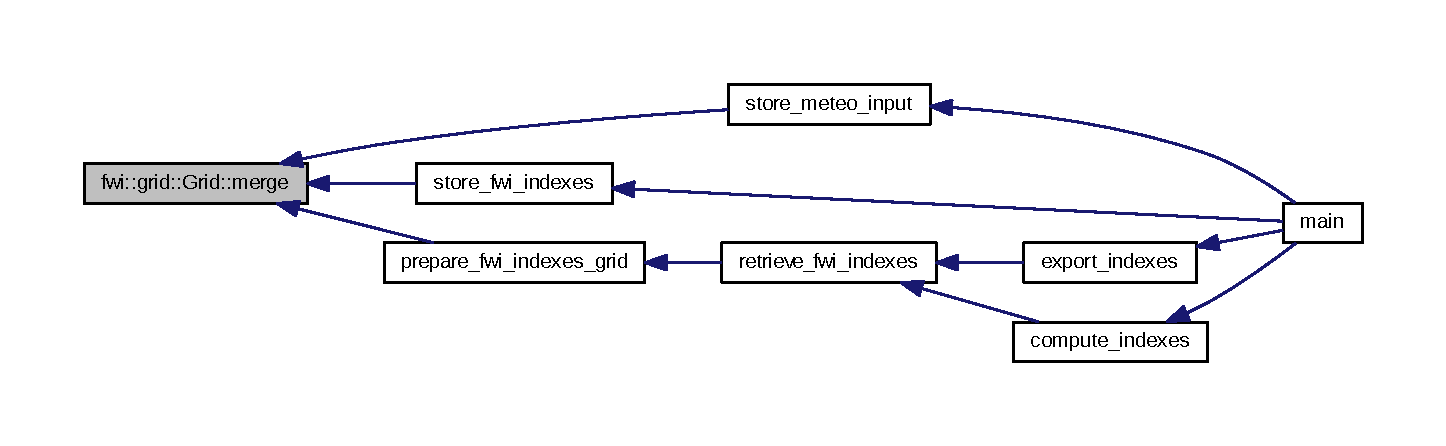
\includegraphics[width=350pt]{classfwi_1_1grid_1_1Grid_a254a6c5a649b7d3a109f67811ef5f356_icgraph}
\end{center}
\end{figure}


\hypertarget{classfwi_1_1grid_1_1Grid_a4892438084efa099f29fbb4fbf5d3e83}{\index{fwi\-::grid\-::\-Grid@{fwi\-::grid\-::\-Grid}!operator()@{operator()}}
\index{operator()@{operator()}!fwi::grid::Grid@{fwi\-::grid\-::\-Grid}}
\subsubsection[{operator()}]{\setlength{\rightskip}{0pt plus 5cm}template$<$typename T $>$ T \& {\bf fwi\-::grid\-::\-Grid}$<$ T $>$\-::operator() (
\begin{DoxyParamCaption}
\item[{int}]{i, }
\item[{int}]{j, }
\item[{int}]{k}
\end{DoxyParamCaption}
)}}\label{classfwi_1_1grid_1_1Grid_a4892438084efa099f29fbb4fbf5d3e83}


grid element access helper 


\begin{DoxyParams}{Parameters}
{\em i} & row number \\
\hline
{\em j} & column number \\
\hline
{\em k} & plane number \\
\hline
\end{DoxyParams}
\begin{DoxyReturn}{Returns}
grid element at row {\itshape i} column {\itshape j} 
\end{DoxyReturn}


Definition at line 1447 of file Grid.\-h.

\hypertarget{classfwi_1_1grid_1_1Grid_a8cbde1277dbb531069c1b579cb10410f}{\index{fwi\-::grid\-::\-Grid@{fwi\-::grid\-::\-Grid}!operator=@{operator=}}
\index{operator=@{operator=}!fwi::grid::Grid@{fwi\-::grid\-::\-Grid}}
\subsubsection[{operator=}]{\setlength{\rightskip}{0pt plus 5cm}template$<$typename T $>$ {\bf Grid}$<$ T $>$ \& {\bf fwi\-::grid\-::\-Grid}$<$ T $>$\-::operator= (
\begin{DoxyParamCaption}
\item[{const {\bf Grid}$<$ T $>$ \&}]{grid}
\end{DoxyParamCaption}
)}}\label{classfwi_1_1grid_1_1Grid_a8cbde1277dbb531069c1b579cb10410f}


grid assignement operator 


\begin{DoxyParams}{Parameters}
{\em grid} & grid to be assigned \\
\hline
\end{DoxyParams}
\begin{DoxyReturn}{Returns}
this grid after assignement 
\end{DoxyReturn}


Definition at line 1455 of file Grid.\-h.

\hypertarget{classfwi_1_1grid_1_1Grid_aafc829b90cb1a0dc6ec9daf425f6b8b7}{\index{fwi\-::grid\-::\-Grid@{fwi\-::grid\-::\-Grid}!read@{read}}
\index{read@{read}!fwi::grid::Grid@{fwi\-::grid\-::\-Grid}}
\subsubsection[{read}]{\setlength{\rightskip}{0pt plus 5cm}template$<$typename T $>$ bool {\bf fwi\-::grid\-::\-Grid}$<$ T $>$\-::read (
\begin{DoxyParamCaption}
{}
\end{DoxyParamCaption}
)}}\label{classfwi_1_1grid_1_1Grid_aafc829b90cb1a0dc6ec9daf425f6b8b7}


reads grid binary file 

\begin{DoxyReturn}{Returns}
true on success else false 
\end{DoxyReturn}


Definition at line 1776 of file Grid.\-h.



Here is the caller graph for this function\-:\nopagebreak
\begin{figure}[H]
\begin{center}
\leavevmode
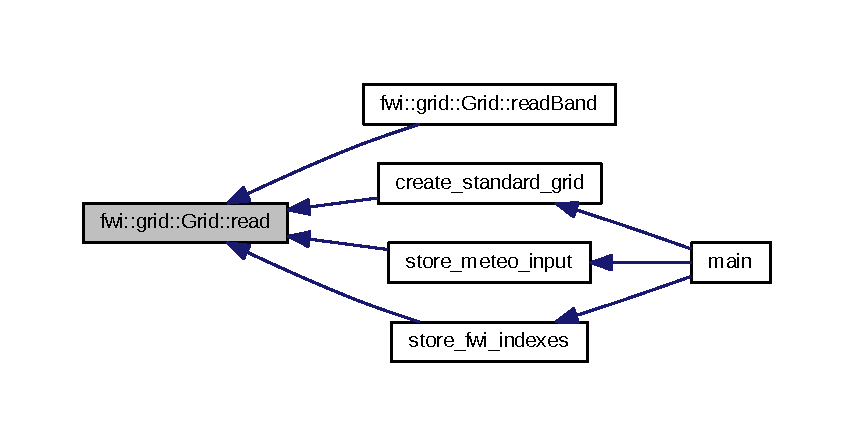
\includegraphics[width=350pt]{classfwi_1_1grid_1_1Grid_aafc829b90cb1a0dc6ec9daf425f6b8b7_icgraph}
\end{center}
\end{figure}


\hypertarget{classfwi_1_1grid_1_1Grid_a07cf7c55e15a35e7b258574a8cda7685}{\index{fwi\-::grid\-::\-Grid@{fwi\-::grid\-::\-Grid}!read\-Band@{read\-Band}}
\index{read\-Band@{read\-Band}!fwi::grid::Grid@{fwi\-::grid\-::\-Grid}}
\subsubsection[{read\-Band}]{\setlength{\rightskip}{0pt plus 5cm}template$<$typename T $>$ bool {\bf fwi\-::grid\-::\-Grid}$<$ T $>$\-::read\-Band (
\begin{DoxyParamCaption}
\item[{ifstream \&}]{in}
\end{DoxyParamCaption}
)\hspace{0.3cm}{\ttfamily [protected]}}}\label{classfwi_1_1grid_1_1Grid_a07cf7c55e15a35e7b258574a8cda7685}


reads data from a grid time band (stream must be opened in binary mode) not appliable to text streams 


\begin{DoxyParams}{Parameters}
{\em in} & input stream \\
\hline
\end{DoxyParams}
\begin{DoxyReturn}{Returns}
true on success else false 
\end{DoxyReturn}


Definition at line 1919 of file Grid.\-h.



Here is the call graph for this function\-:\nopagebreak
\begin{figure}[H]
\begin{center}
\leavevmode
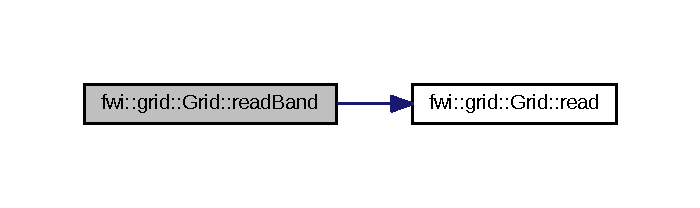
\includegraphics[width=336pt]{classfwi_1_1grid_1_1Grid_a07cf7c55e15a35e7b258574a8cda7685_cgraph}
\end{center}
\end{figure}


\hypertarget{classfwi_1_1grid_1_1Grid_a9f941bf44e6f27620181cd7b406150e2}{\index{fwi\-::grid\-::\-Grid@{fwi\-::grid\-::\-Grid}!read\-Bin@{read\-Bin}}
\index{read\-Bin@{read\-Bin}!fwi::grid::Grid@{fwi\-::grid\-::\-Grid}}
\subsubsection[{read\-Bin}]{\setlength{\rightskip}{0pt plus 5cm}template$<$typename T $>$ bool {\bf fwi\-::grid\-::\-Grid}$<$ T $>$\-::read\-Bin (
\begin{DoxyParamCaption}
\item[{ifstream \&}]{in}
\end{DoxyParamCaption}
)\hspace{0.3cm}{\ttfamily [protected]}}}\label{classfwi_1_1grid_1_1Grid_a9f941bf44e6f27620181cd7b406150e2}


reads grid data from binary file 


\begin{DoxyParams}{Parameters}
{\em in} & input stream \\
\hline
\end{DoxyParams}
\begin{DoxyReturn}{Returns}
true on success else false 
\end{DoxyReturn}


Definition at line 1864 of file Grid.\-h.

\hypertarget{classfwi_1_1grid_1_1Grid_a34cc464d768d11a63f6918e6a39e0415}{\index{fwi\-::grid\-::\-Grid@{fwi\-::grid\-::\-Grid}!read\-Ctrl@{read\-Ctrl}}
\index{read\-Ctrl@{read\-Ctrl}!fwi::grid::Grid@{fwi\-::grid\-::\-Grid}}
\subsubsection[{read\-Ctrl}]{\setlength{\rightskip}{0pt plus 5cm}template$<$typename T $>$ bool {\bf fwi\-::grid\-::\-Grid}$<$ T $>$\-::read\-Ctrl (
\begin{DoxyParamCaption}
\item[{ifstream \&}]{in}
\end{DoxyParamCaption}
)}}\label{classfwi_1_1grid_1_1Grid_a34cc464d768d11a63f6918e6a39e0415}


reads grid control file 


\begin{DoxyParams}{Parameters}
{\em in} & input stream \\
\hline
\end{DoxyParams}
\begin{DoxyReturn}{Returns}
true on success else false 
\end{DoxyReturn}


Definition at line 1770 of file Grid.\-h.

\hypertarget{classfwi_1_1grid_1_1Grid_ac6262b427ff75bcfac1d118afccb1c71}{\index{fwi\-::grid\-::\-Grid@{fwi\-::grid\-::\-Grid}!read\-Txt@{read\-Txt}}
\index{read\-Txt@{read\-Txt}!fwi::grid::Grid@{fwi\-::grid\-::\-Grid}}
\subsubsection[{read\-Txt}]{\setlength{\rightskip}{0pt plus 5cm}template$<$typename T $>$ bool {\bf fwi\-::grid\-::\-Grid}$<$ T $>$\-::read\-Txt (
\begin{DoxyParamCaption}
\item[{ifstream \&}]{in}
\end{DoxyParamCaption}
)\hspace{0.3cm}{\ttfamily [protected]}}}\label{classfwi_1_1grid_1_1Grid_ac6262b427ff75bcfac1d118afccb1c71}


reads grid data from text file 


\begin{DoxyParams}{Parameters}
{\em in} & input stream \\
\hline
\end{DoxyParams}
\begin{DoxyReturn}{Returns}
true on success else false 
\end{DoxyReturn}


Definition at line 1819 of file Grid.\-h.

\hypertarget{classfwi_1_1grid_1_1Grid_a653fc4a3630fbcfc92229b42fea9ab77}{\index{fwi\-::grid\-::\-Grid@{fwi\-::grid\-::\-Grid}!retrieve@{retrieve}}
\index{retrieve@{retrieve}!fwi::grid::Grid@{fwi\-::grid\-::\-Grid}}
\subsubsection[{retrieve}]{\setlength{\rightskip}{0pt plus 5cm}template$<$typename T $>$ bool {\bf fwi\-::grid\-::\-Grid}$<$ T $>$\-::retrieve (
\begin{DoxyParamCaption}
\item[{P\-Gconn $\ast$}]{conn}
\end{DoxyParamCaption}
)}}\label{classfwi_1_1grid_1_1Grid_a653fc4a3630fbcfc92229b42fea9ab77}


retrieves grid from database 


\begin{DoxyParams}{Parameters}
{\em conn} & postgresql connection \\
\hline
\end{DoxyParams}
\begin{DoxyReturn}{Returns}
true on success else false 
\end{DoxyReturn}
\begin{DoxySeeAlso}{See also}
postgresql documentation at \href{http://www.postgresql.org/}{\tt http\-://www.\-postgresql.\-org/} 
\end{DoxySeeAlso}


Definition at line 2352 of file Grid.\-h.



Here is the caller graph for this function\-:\nopagebreak
\begin{figure}[H]
\begin{center}
\leavevmode
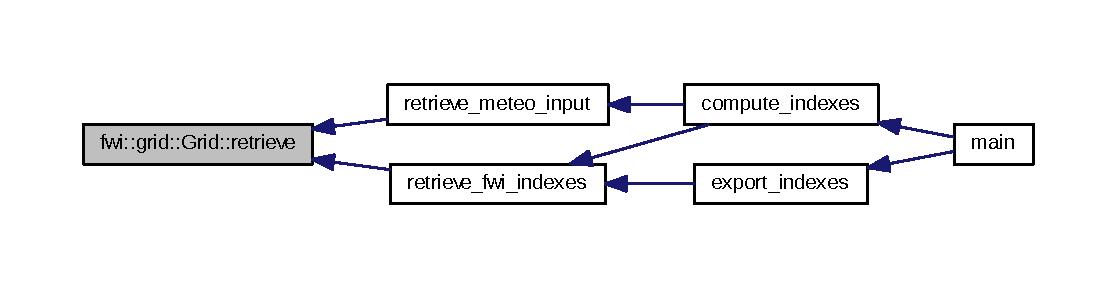
\includegraphics[width=350pt]{classfwi_1_1grid_1_1Grid_a653fc4a3630fbcfc92229b42fea9ab77_icgraph}
\end{center}
\end{figure}


\hypertarget{classfwi_1_1grid_1_1Grid_a8ee0c76d69626d72bc385c5cb3cdf268}{\index{fwi\-::grid\-::\-Grid@{fwi\-::grid\-::\-Grid}!set\-Cols@{set\-Cols}}
\index{set\-Cols@{set\-Cols}!fwi::grid::Grid@{fwi\-::grid\-::\-Grid}}
\subsubsection[{set\-Cols}]{\setlength{\rightskip}{0pt plus 5cm}template$<$typename T $>$ void {\bf fwi\-::grid\-::\-Grid}$<$ T $>$\-::set\-Cols (
\begin{DoxyParamCaption}
\item[{int}]{cols}
\end{DoxyParamCaption}
)}}\label{classfwi_1_1grid_1_1Grid_a8ee0c76d69626d72bc385c5cb3cdf268}


grid columns number setter 


\begin{DoxyParams}{Parameters}
{\em cols} & new columns number value \\
\hline
\end{DoxyParams}


Definition at line 1274 of file Grid.\-h.



Here is the caller graph for this function\-:\nopagebreak
\begin{figure}[H]
\begin{center}
\leavevmode
\includegraphics[width=350pt]{classfwi_1_1grid_1_1Grid_a8ee0c76d69626d72bc385c5cb3cdf268_icgraph}
\end{center}
\end{figure}


\hypertarget{classfwi_1_1grid_1_1Grid_a5beeb3bf022ee1dec908f76bf1b7ff5d}{\index{fwi\-::grid\-::\-Grid@{fwi\-::grid\-::\-Grid}!set\-Ctl\-Path@{set\-Ctl\-Path}}
\index{set\-Ctl\-Path@{set\-Ctl\-Path}!fwi::grid::Grid@{fwi\-::grid\-::\-Grid}}
\subsubsection[{set\-Ctl\-Path}]{\setlength{\rightskip}{0pt plus 5cm}template$<$typename T $>$ void {\bf fwi\-::grid\-::\-Grid}$<$ T $>$\-::set\-Ctl\-Path (
\begin{DoxyParamCaption}
\item[{std\-::string}]{filepath}
\end{DoxyParamCaption}
)}}\label{classfwi_1_1grid_1_1Grid_a5beeb3bf022ee1dec908f76bf1b7ff5d}


grid ctl file path setter 


\begin{DoxyParams}{Parameters}
{\em filepath} & new ctl file path value \\
\hline
\end{DoxyParams}


Definition at line 1304 of file Grid.\-h.

\hypertarget{classfwi_1_1grid_1_1Grid_a38c849794390871a95b8c7dbe505e00d}{\index{fwi\-::grid\-::\-Grid@{fwi\-::grid\-::\-Grid}!set\-Date@{set\-Date}}
\index{set\-Date@{set\-Date}!fwi::grid::Grid@{fwi\-::grid\-::\-Grid}}
\subsubsection[{set\-Date}]{\setlength{\rightskip}{0pt plus 5cm}template$<$typename T $>$ void {\bf fwi\-::grid\-::\-Grid}$<$ T $>$\-::set\-Date (
\begin{DoxyParamCaption}
\item[{std\-::string}]{date}
\end{DoxyParamCaption}
)}}\label{classfwi_1_1grid_1_1Grid_a38c849794390871a95b8c7dbe505e00d}


date setter 


\begin{DoxyParams}{Parameters}
{\em date} & date value expressed as Y\-Y\-Y\-Y\-M\-M\-D\-D \\
\hline
\end{DoxyParams}


Definition at line 1286 of file Grid.\-h.



Here is the caller graph for this function\-:\nopagebreak
\begin{figure}[H]
\begin{center}
\leavevmode
\includegraphics[width=350pt]{classfwi_1_1grid_1_1Grid_a38c849794390871a95b8c7dbe505e00d_icgraph}
\end{center}
\end{figure}


\hypertarget{classfwi_1_1grid_1_1Grid_ac7df5d5cc5b9d184c5eceb03737bb598}{\index{fwi\-::grid\-::\-Grid@{fwi\-::grid\-::\-Grid}!set\-Dat\-Path@{set\-Dat\-Path}}
\index{set\-Dat\-Path@{set\-Dat\-Path}!fwi::grid::Grid@{fwi\-::grid\-::\-Grid}}
\subsubsection[{set\-Dat\-Path}]{\setlength{\rightskip}{0pt plus 5cm}template$<$typename T $>$ void {\bf fwi\-::grid\-::\-Grid}$<$ T $>$\-::set\-Dat\-Path (
\begin{DoxyParamCaption}
\item[{std\-::string}]{filepath}
\end{DoxyParamCaption}
)}}\label{classfwi_1_1grid_1_1Grid_ac7df5d5cc5b9d184c5eceb03737bb598}


grid dat file path setter 


\begin{DoxyParams}{Parameters}
{\em filepath} & new dat file path value \\
\hline
\end{DoxyParams}


Definition at line 1310 of file Grid.\-h.



Here is the caller graph for this function\-:\nopagebreak
\begin{figure}[H]
\begin{center}
\leavevmode
\includegraphics[width=350pt]{classfwi_1_1grid_1_1Grid_ac7df5d5cc5b9d184c5eceb03737bb598_icgraph}
\end{center}
\end{figure}


\hypertarget{classfwi_1_1grid_1_1Grid_ab138cac6c49037fc1b911a7a7d2eb437}{\index{fwi\-::grid\-::\-Grid@{fwi\-::grid\-::\-Grid}!set\-Export\-Ctl\-Path@{set\-Export\-Ctl\-Path}}
\index{set\-Export\-Ctl\-Path@{set\-Export\-Ctl\-Path}!fwi::grid::Grid@{fwi\-::grid\-::\-Grid}}
\subsubsection[{set\-Export\-Ctl\-Path}]{\setlength{\rightskip}{0pt plus 5cm}template$<$typename T $>$ void {\bf fwi\-::grid\-::\-Grid}$<$ T $>$\-::set\-Export\-Ctl\-Path (
\begin{DoxyParamCaption}
\item[{std\-::string}]{filepath}
\end{DoxyParamCaption}
)}}\label{classfwi_1_1grid_1_1Grid_ab138cac6c49037fc1b911a7a7d2eb437}


grid export ctl file path setter 


\begin{DoxyParams}{Parameters}
{\em filepath} & new ctl export file path value \\
\hline
\end{DoxyParams}


Definition at line 1316 of file Grid.\-h.

\hypertarget{classfwi_1_1grid_1_1Grid_a84899af1e9496f79a7cf43459c62c9bc}{\index{fwi\-::grid\-::\-Grid@{fwi\-::grid\-::\-Grid}!set\-Export\-Dat\-Path@{set\-Export\-Dat\-Path}}
\index{set\-Export\-Dat\-Path@{set\-Export\-Dat\-Path}!fwi::grid::Grid@{fwi\-::grid\-::\-Grid}}
\subsubsection[{set\-Export\-Dat\-Path}]{\setlength{\rightskip}{0pt plus 5cm}template$<$typename T $>$ void {\bf fwi\-::grid\-::\-Grid}$<$ T $>$\-::set\-Export\-Dat\-Path (
\begin{DoxyParamCaption}
\item[{std\-::string}]{filepath}
\end{DoxyParamCaption}
)}}\label{classfwi_1_1grid_1_1Grid_a84899af1e9496f79a7cf43459c62c9bc}


grid export dat file path setter 


\begin{DoxyParams}{Parameters}
{\em filepath} & new dat export file path value \\
\hline
\end{DoxyParams}


Definition at line 1322 of file Grid.\-h.

\hypertarget{classfwi_1_1grid_1_1Grid_acfa22cf6901ee071064d5dccc255f5ed}{\index{fwi\-::grid\-::\-Grid@{fwi\-::grid\-::\-Grid}!set\-Fields@{set\-Fields}}
\index{set\-Fields@{set\-Fields}!fwi::grid::Grid@{fwi\-::grid\-::\-Grid}}
\subsubsection[{set\-Fields}]{\setlength{\rightskip}{0pt plus 5cm}template$<$typename T $>$ void {\bf fwi\-::grid\-::\-Grid}$<$ T $>$\-::set\-Fields (
\begin{DoxyParamCaption}
\item[{{\bf Grid\-Fields} $\ast$}]{fields}
\end{DoxyParamCaption}
)}}\label{classfwi_1_1grid_1_1Grid_acfa22cf6901ee071064d5dccc255f5ed}


grid fields list setter 


\begin{DoxyParams}{Parameters}
{\em fields} & new grid fields list \\
\hline
\end{DoxyParams}


Definition at line 1437 of file Grid.\-h.

\hypertarget{classfwi_1_1grid_1_1Grid_a15e1fd1e87919bba2971a6fe66566f43}{\index{fwi\-::grid\-::\-Grid@{fwi\-::grid\-::\-Grid}!set\-File\-Name\-Date\-Offset@{set\-File\-Name\-Date\-Offset}}
\index{set\-File\-Name\-Date\-Offset@{set\-File\-Name\-Date\-Offset}!fwi::grid::Grid@{fwi\-::grid\-::\-Grid}}
\subsubsection[{set\-File\-Name\-Date\-Offset}]{\setlength{\rightskip}{0pt plus 5cm}template$<$typename T $>$ void {\bf fwi\-::grid\-::\-Grid}$<$ T $>$\-::set\-File\-Name\-Date\-Offset (
\begin{DoxyParamCaption}
\item[{int}]{offset}
\end{DoxyParamCaption}
)}}\label{classfwi_1_1grid_1_1Grid_a15e1fd1e87919bba2971a6fe66566f43}


grid file name date offset setter 


\begin{DoxyParams}{Parameters}
{\em offset} & file name date offset value \\
\hline
\end{DoxyParams}


Definition at line 1364 of file Grid.\-h.

\hypertarget{classfwi_1_1grid_1_1Grid_a4fe86c25ec42f48f70d2353721e9aeed}{\index{fwi\-::grid\-::\-Grid@{fwi\-::grid\-::\-Grid}!set\-I\-O\-Format@{set\-I\-O\-Format}}
\index{set\-I\-O\-Format@{set\-I\-O\-Format}!fwi::grid::Grid@{fwi\-::grid\-::\-Grid}}
\subsubsection[{set\-I\-O\-Format}]{\setlength{\rightskip}{0pt plus 5cm}template$<$typename T $>$ void {\bf fwi\-::grid\-::\-Grid}$<$ T $>$\-::set\-I\-O\-Format (
\begin{DoxyParamCaption}
\item[{int}]{format}
\end{DoxyParamCaption}
)}}\label{classfwi_1_1grid_1_1Grid_a4fe86c25ec42f48f70d2353721e9aeed}


grid I/\-O format setter 


\begin{DoxyParams}{Parameters}
{\em format} & new I/\-O format value \\
\hline
\end{DoxyParams}


Definition at line 1370 of file Grid.\-h.

\hypertarget{classfwi_1_1grid_1_1Grid_aefe04321df7e26e6510293846d93f983}{\index{fwi\-::grid\-::\-Grid@{fwi\-::grid\-::\-Grid}!set\-Rows@{set\-Rows}}
\index{set\-Rows@{set\-Rows}!fwi::grid::Grid@{fwi\-::grid\-::\-Grid}}
\subsubsection[{set\-Rows}]{\setlength{\rightskip}{0pt plus 5cm}template$<$typename T $>$ void {\bf fwi\-::grid\-::\-Grid}$<$ T $>$\-::set\-Rows (
\begin{DoxyParamCaption}
\item[{int}]{rows}
\end{DoxyParamCaption}
)}}\label{classfwi_1_1grid_1_1Grid_aefe04321df7e26e6510293846d93f983}


grid rows number setter 


\begin{DoxyParams}{Parameters}
{\em rows} & new rows number value \\
\hline
\end{DoxyParams}


Definition at line 1268 of file Grid.\-h.



Here is the caller graph for this function\-:\nopagebreak
\begin{figure}[H]
\begin{center}
\leavevmode
\includegraphics[width=350pt]{classfwi_1_1grid_1_1Grid_aefe04321df7e26e6510293846d93f983_icgraph}
\end{center}
\end{figure}


\hypertarget{classfwi_1_1grid_1_1Grid_ac0fe4e20d56ed5507f62c1d3e6502f68}{\index{fwi\-::grid\-::\-Grid@{fwi\-::grid\-::\-Grid}!set\-Slot\-Size@{set\-Slot\-Size}}
\index{set\-Slot\-Size@{set\-Slot\-Size}!fwi::grid::Grid@{fwi\-::grid\-::\-Grid}}
\subsubsection[{set\-Slot\-Size}]{\setlength{\rightskip}{0pt plus 5cm}template$<$typename T $>$ void {\bf fwi\-::grid\-::\-Grid}$<$ T $>$\-::set\-Slot\-Size (
\begin{DoxyParamCaption}
\item[{int}]{slot\-Size}
\end{DoxyParamCaption}
)}}\label{classfwi_1_1grid_1_1Grid_ac0fe4e20d56ed5507f62c1d3e6502f68}


grid slot size setter 


\begin{DoxyParams}{Parameters}
{\em slot\-Size} & new grid slot size value \\
\hline
\end{DoxyParams}


Definition at line 1431 of file Grid.\-h.

\hypertarget{classfwi_1_1grid_1_1Grid_aff98dae08698282b2a1661810856e673}{\index{fwi\-::grid\-::\-Grid@{fwi\-::grid\-::\-Grid}!set\-S\-R\-I\-D@{set\-S\-R\-I\-D}}
\index{set\-S\-R\-I\-D@{set\-S\-R\-I\-D}!fwi::grid::Grid@{fwi\-::grid\-::\-Grid}}
\subsubsection[{set\-S\-R\-I\-D}]{\setlength{\rightskip}{0pt plus 5cm}template$<$typename T $>$ void {\bf fwi\-::grid\-::\-Grid}$<$ T $>$\-::set\-S\-R\-I\-D (
\begin{DoxyParamCaption}
\item[{int}]{srid}
\end{DoxyParamCaption}
)}}\label{classfwi_1_1grid_1_1Grid_aff98dae08698282b2a1661810856e673}


grid srid setter 


\begin{DoxyParams}{Parameters}
{\em srid} & new srid value \\
\hline
\end{DoxyParams}


Definition at line 1419 of file Grid.\-h.

\hypertarget{classfwi_1_1grid_1_1Grid_a9e75d99eef25e9a401aadd71ad646e08}{\index{fwi\-::grid\-::\-Grid@{fwi\-::grid\-::\-Grid}!set\-Start\-Time@{set\-Start\-Time}}
\index{set\-Start\-Time@{set\-Start\-Time}!fwi::grid::Grid@{fwi\-::grid\-::\-Grid}}
\subsubsection[{set\-Start\-Time}]{\setlength{\rightskip}{0pt plus 5cm}template$<$typename T $>$ void {\bf fwi\-::grid\-::\-Grid}$<$ T $>$\-::set\-Start\-Time (
\begin{DoxyParamCaption}
\item[{std\-::string}]{t}
\end{DoxyParamCaption}
)}}\label{classfwi_1_1grid_1_1Grid_a9e75d99eef25e9a401aadd71ad646e08}


grid start time setter 


\begin{DoxyParams}{Parameters}
{\em t} & grid new start time value in Gr\-A\-D\-S format \\
\hline
\end{DoxyParams}
\begin{DoxySeeAlso}{See also}
\href{http://www.iges.org/grads/}{\tt http\-://www.\-iges.\-org/grads/} 
\end{DoxySeeAlso}


Definition at line 1352 of file Grid.\-h.

\hypertarget{classfwi_1_1grid_1_1Grid_a78f4a38e86a245ee62769e5f37bff1c6}{\index{fwi\-::grid\-::\-Grid@{fwi\-::grid\-::\-Grid}!set\-Table@{set\-Table}}
\index{set\-Table@{set\-Table}!fwi::grid::Grid@{fwi\-::grid\-::\-Grid}}
\subsubsection[{set\-Table}]{\setlength{\rightskip}{0pt plus 5cm}template$<$typename T $>$ void {\bf fwi\-::grid\-::\-Grid}$<$ T $>$\-::set\-Table (
\begin{DoxyParamCaption}
\item[{std\-::string}]{table}
\end{DoxyParamCaption}
)}}\label{classfwi_1_1grid_1_1Grid_a78f4a38e86a245ee62769e5f37bff1c6}


grid table name setter 


\begin{DoxyParams}{Parameters}
{\em table} & new table name value \\
\hline
\end{DoxyParams}


Definition at line 1280 of file Grid.\-h.



Here is the caller graph for this function\-:\nopagebreak
\begin{figure}[H]
\begin{center}
\leavevmode
\includegraphics[width=350pt]{classfwi_1_1grid_1_1Grid_a78f4a38e86a245ee62769e5f37bff1c6_icgraph}
\end{center}
\end{figure}


\hypertarget{classfwi_1_1grid_1_1Grid_a3ed06b6c1a2ea5596c78256b2b872d81}{\index{fwi\-::grid\-::\-Grid@{fwi\-::grid\-::\-Grid}!set\-Time\-Band@{set\-Time\-Band}}
\index{set\-Time\-Band@{set\-Time\-Band}!fwi::grid::Grid@{fwi\-::grid\-::\-Grid}}
\subsubsection[{set\-Time\-Band}]{\setlength{\rightskip}{0pt plus 5cm}template$<$typename T $>$ void {\bf fwi\-::grid\-::\-Grid}$<$ T $>$\-::set\-Time\-Band (
\begin{DoxyParamCaption}
\item[{int}]{band}
\end{DoxyParamCaption}
)}}\label{classfwi_1_1grid_1_1Grid_a3ed06b6c1a2ea5596c78256b2b872d81}


grid time band setter 


\begin{DoxyParams}{Parameters}
{\em band} & new time band value \\
\hline
\end{DoxyParams}


Definition at line 1340 of file Grid.\-h.

\hypertarget{classfwi_1_1grid_1_1Grid_a19b83ec99e6280c7da1ad6b08cc3b921}{\index{fwi\-::grid\-::\-Grid@{fwi\-::grid\-::\-Grid}!set\-Time\-Bands\-Number@{set\-Time\-Bands\-Number}}
\index{set\-Time\-Bands\-Number@{set\-Time\-Bands\-Number}!fwi::grid::Grid@{fwi\-::grid\-::\-Grid}}
\subsubsection[{set\-Time\-Bands\-Number}]{\setlength{\rightskip}{0pt plus 5cm}template$<$typename T $>$ void {\bf fwi\-::grid\-::\-Grid}$<$ T $>$\-::set\-Time\-Bands\-Number (
\begin{DoxyParamCaption}
\item[{int}]{bands\-Number}
\end{DoxyParamCaption}
)}}\label{classfwi_1_1grid_1_1Grid_a19b83ec99e6280c7da1ad6b08cc3b921}


grid time bands number setter 


\begin{DoxyParams}{Parameters}
{\em bands\-Number} & new time bands number value \\
\hline
\end{DoxyParams}


Definition at line 1346 of file Grid.\-h.

\hypertarget{classfwi_1_1grid_1_1Grid_afc7b78751770989300220237fcae5256}{\index{fwi\-::grid\-::\-Grid@{fwi\-::grid\-::\-Grid}!set\-Time\-Increment@{set\-Time\-Increment}}
\index{set\-Time\-Increment@{set\-Time\-Increment}!fwi::grid::Grid@{fwi\-::grid\-::\-Grid}}
\subsubsection[{set\-Time\-Increment}]{\setlength{\rightskip}{0pt plus 5cm}template$<$typename T $>$ void {\bf fwi\-::grid\-::\-Grid}$<$ T $>$\-::set\-Time\-Increment (
\begin{DoxyParamCaption}
\item[{std\-::string}]{increment}
\end{DoxyParamCaption}
)}}\label{classfwi_1_1grid_1_1Grid_afc7b78751770989300220237fcae5256}


grid time increment setter 


\begin{DoxyParams}{Parameters}
{\em increment} & new time increment value \\
\hline
\end{DoxyParams}


Definition at line 1358 of file Grid.\-h.

\hypertarget{classfwi_1_1grid_1_1Grid_a0cdb2357ad4279db9bc990bb17eecef0}{\index{fwi\-::grid\-::\-Grid@{fwi\-::grid\-::\-Grid}!set\-Title@{set\-Title}}
\index{set\-Title@{set\-Title}!fwi::grid::Grid@{fwi\-::grid\-::\-Grid}}
\subsubsection[{set\-Title}]{\setlength{\rightskip}{0pt plus 5cm}template$<$typename T $>$ void {\bf fwi\-::grid\-::\-Grid}$<$ T $>$\-::set\-Title (
\begin{DoxyParamCaption}
\item[{std\-::string}]{title}
\end{DoxyParamCaption}
)}}\label{classfwi_1_1grid_1_1Grid_a0cdb2357ad4279db9bc990bb17eecef0}


grid title setter 


\begin{DoxyParams}{Parameters}
{\em title} & new title value \\
\hline
\end{DoxyParams}


Definition at line 1328 of file Grid.\-h.

\hypertarget{classfwi_1_1grid_1_1Grid_a6e7dc5bcf9d26a25289a324b2d4f8926}{\index{fwi\-::grid\-::\-Grid@{fwi\-::grid\-::\-Grid}!set\-Type@{set\-Type}}
\index{set\-Type@{set\-Type}!fwi::grid::Grid@{fwi\-::grid\-::\-Grid}}
\subsubsection[{set\-Type}]{\setlength{\rightskip}{0pt plus 5cm}template$<$typename T $>$ void {\bf fwi\-::grid\-::\-Grid}$<$ T $>$\-::set\-Type (
\begin{DoxyParamCaption}
\item[{int}]{type}
\end{DoxyParamCaption}
)}}\label{classfwi_1_1grid_1_1Grid_a6e7dc5bcf9d26a25289a324b2d4f8926}


grid type setter 


\begin{DoxyParams}{Parameters}
{\em type} & new type value \\
\hline
\end{DoxyParams}


Definition at line 1334 of file Grid.\-h.



Here is the caller graph for this function\-:\nopagebreak
\begin{figure}[H]
\begin{center}
\leavevmode
\includegraphics[width=350pt]{classfwi_1_1grid_1_1Grid_a6e7dc5bcf9d26a25289a324b2d4f8926_icgraph}
\end{center}
\end{figure}


\hypertarget{classfwi_1_1grid_1_1Grid_ad1090e0ab615bf979eb72bbc55ca6fb3}{\index{fwi\-::grid\-::\-Grid@{fwi\-::grid\-::\-Grid}!set\-Undef\-Value@{set\-Undef\-Value}}
\index{set\-Undef\-Value@{set\-Undef\-Value}!fwi::grid::Grid@{fwi\-::grid\-::\-Grid}}
\subsubsection[{set\-Undef\-Value}]{\setlength{\rightskip}{0pt plus 5cm}template$<$typename T $>$ void {\bf fwi\-::grid\-::\-Grid}$<$ T $>$\-::set\-Undef\-Value (
\begin{DoxyParamCaption}
\item[{float}]{undef\-Value}
\end{DoxyParamCaption}
)}}\label{classfwi_1_1grid_1_1Grid_ad1090e0ab615bf979eb72bbc55ca6fb3}


grid undefined value setter 


\begin{DoxyParams}{Parameters}
{\em undef\-Value} & new grid undefined value \\
\hline
\end{DoxyParams}


Definition at line 1425 of file Grid.\-h.



Here is the caller graph for this function\-:\nopagebreak
\begin{figure}[H]
\begin{center}
\leavevmode
\includegraphics[width=350pt]{classfwi_1_1grid_1_1Grid_ad1090e0ab615bf979eb72bbc55ca6fb3_icgraph}
\end{center}
\end{figure}


\hypertarget{classfwi_1_1grid_1_1Grid_ab063dbc1b9e23f21c27611851390de23}{\index{fwi\-::grid\-::\-Grid@{fwi\-::grid\-::\-Grid}!set\-Var\-Num@{set\-Var\-Num}}
\index{set\-Var\-Num@{set\-Var\-Num}!fwi::grid::Grid@{fwi\-::grid\-::\-Grid}}
\subsubsection[{set\-Var\-Num}]{\setlength{\rightskip}{0pt plus 5cm}template$<$typename T $>$ void {\bf fwi\-::grid\-::\-Grid}$<$ T $>$\-::set\-Var\-Num (
\begin{DoxyParamCaption}
\item[{int}]{varnum}
\end{DoxyParamCaption}
)}}\label{classfwi_1_1grid_1_1Grid_ab063dbc1b9e23f21c27611851390de23}


grid variables number setter 

\begin{DoxyVerb}     Implies grid resize. Elements are preserved only if the new value for
     <i>varNum</i> is greater than or equal to the old one.
\end{DoxyVerb}



\begin{DoxyParams}{Parameters}
{\em varnum} & new variables number value \\
\hline
\end{DoxyParams}


Definition at line 1412 of file Grid.\-h.



Here is the caller graph for this function\-:\nopagebreak
\begin{figure}[H]
\begin{center}
\leavevmode
\includegraphics[width=350pt]{classfwi_1_1grid_1_1Grid_ab063dbc1b9e23f21c27611851390de23_icgraph}
\end{center}
\end{figure}


\hypertarget{classfwi_1_1grid_1_1Grid_a58a313c74d268e1a892877dbe97782e0}{\index{fwi\-::grid\-::\-Grid@{fwi\-::grid\-::\-Grid}!set\-X\-Dir@{set\-X\-Dir}}
\index{set\-X\-Dir@{set\-X\-Dir}!fwi::grid::Grid@{fwi\-::grid\-::\-Grid}}
\subsubsection[{set\-X\-Dir}]{\setlength{\rightskip}{0pt plus 5cm}template$<$typename T $>$ void {\bf fwi\-::grid\-::\-Grid}$<$ T $>$\-::set\-X\-Dir (
\begin{DoxyParamCaption}
\item[{C\-O\-O\-R\-D\-I\-N\-A\-T\-E\-\_\-\-D\-I\-R\-E\-C\-T\-I\-O\-N}]{x\-Dir}
\end{DoxyParamCaption}
)}}\label{classfwi_1_1grid_1_1Grid_a58a313c74d268e1a892877dbe97782e0}


x\-Dir setter 


\begin{DoxyParams}{Parameters}
{\em x\-Dir} & new x\-Dir value \\
\hline
\end{DoxyParams}


Definition at line 1400 of file Grid.\-h.



Here is the caller graph for this function\-:\nopagebreak
\begin{figure}[H]
\begin{center}
\leavevmode
\includegraphics[width=350pt]{classfwi_1_1grid_1_1Grid_a58a313c74d268e1a892877dbe97782e0_icgraph}
\end{center}
\end{figure}


\hypertarget{classfwi_1_1grid_1_1Grid_a3e358d51e63374a9174fcff2206ba9d1}{\index{fwi\-::grid\-::\-Grid@{fwi\-::grid\-::\-Grid}!set\-X\-Start@{set\-X\-Start}}
\index{set\-X\-Start@{set\-X\-Start}!fwi::grid::Grid@{fwi\-::grid\-::\-Grid}}
\subsubsection[{set\-X\-Start}]{\setlength{\rightskip}{0pt plus 5cm}template$<$typename T $>$ void {\bf fwi\-::grid\-::\-Grid}$<$ T $>$\-::set\-X\-Start (
\begin{DoxyParamCaption}
\item[{float}]{xstart}
\end{DoxyParamCaption}
)}}\label{classfwi_1_1grid_1_1Grid_a3e358d51e63374a9174fcff2206ba9d1}


grid start x coordinate setter 


\begin{DoxyParams}{Parameters}
{\em xstart} & new xtsrat value \\
\hline
\end{DoxyParams}


Definition at line 1376 of file Grid.\-h.

\hypertarget{classfwi_1_1grid_1_1Grid_a442147db5a15cb302bc640041bc42d49}{\index{fwi\-::grid\-::\-Grid@{fwi\-::grid\-::\-Grid}!set\-X\-Step@{set\-X\-Step}}
\index{set\-X\-Step@{set\-X\-Step}!fwi::grid::Grid@{fwi\-::grid\-::\-Grid}}
\subsubsection[{set\-X\-Step}]{\setlength{\rightskip}{0pt plus 5cm}template$<$typename T $>$ void {\bf fwi\-::grid\-::\-Grid}$<$ T $>$\-::set\-X\-Step (
\begin{DoxyParamCaption}
\item[{float}]{xstep}
\end{DoxyParamCaption}
)}}\label{classfwi_1_1grid_1_1Grid_a442147db5a15cb302bc640041bc42d49}


grid step in x direction setter 


\begin{DoxyParams}{Parameters}
{\em xstep} & new xstep value \\
\hline
\end{DoxyParams}


Definition at line 1382 of file Grid.\-h.

\hypertarget{classfwi_1_1grid_1_1Grid_a8ee82188e306a47c14813024513bd56e}{\index{fwi\-::grid\-::\-Grid@{fwi\-::grid\-::\-Grid}!set\-Y\-Dir@{set\-Y\-Dir}}
\index{set\-Y\-Dir@{set\-Y\-Dir}!fwi::grid::Grid@{fwi\-::grid\-::\-Grid}}
\subsubsection[{set\-Y\-Dir}]{\setlength{\rightskip}{0pt plus 5cm}template$<$typename T $>$ void {\bf fwi\-::grid\-::\-Grid}$<$ T $>$\-::set\-Y\-Dir (
\begin{DoxyParamCaption}
\item[{C\-O\-O\-R\-D\-I\-N\-A\-T\-E\-\_\-\-D\-I\-R\-E\-C\-T\-I\-O\-N}]{y\-Dir}
\end{DoxyParamCaption}
)}}\label{classfwi_1_1grid_1_1Grid_a8ee82188e306a47c14813024513bd56e}


y\-Dir setter 


\begin{DoxyParams}{Parameters}
{\em y\-Dir} & new y\-Dir value \\
\hline
\end{DoxyParams}


Definition at line 1406 of file Grid.\-h.

\hypertarget{classfwi_1_1grid_1_1Grid_a9a22e6a8991396d957900b33b9db6558}{\index{fwi\-::grid\-::\-Grid@{fwi\-::grid\-::\-Grid}!set\-Y\-Start@{set\-Y\-Start}}
\index{set\-Y\-Start@{set\-Y\-Start}!fwi::grid::Grid@{fwi\-::grid\-::\-Grid}}
\subsubsection[{set\-Y\-Start}]{\setlength{\rightskip}{0pt plus 5cm}template$<$typename T $>$ void {\bf fwi\-::grid\-::\-Grid}$<$ T $>$\-::set\-Y\-Start (
\begin{DoxyParamCaption}
\item[{float}]{ystart}
\end{DoxyParamCaption}
)}}\label{classfwi_1_1grid_1_1Grid_a9a22e6a8991396d957900b33b9db6558}


grid start y coordinate setter 


\begin{DoxyParams}{Parameters}
{\em ystart} & new ystart value \\
\hline
\end{DoxyParams}


Definition at line 1388 of file Grid.\-h.

\hypertarget{classfwi_1_1grid_1_1Grid_aeb84b8b6061243f47f6cea19bda8acbc}{\index{fwi\-::grid\-::\-Grid@{fwi\-::grid\-::\-Grid}!set\-Y\-Step@{set\-Y\-Step}}
\index{set\-Y\-Step@{set\-Y\-Step}!fwi::grid::Grid@{fwi\-::grid\-::\-Grid}}
\subsubsection[{set\-Y\-Step}]{\setlength{\rightskip}{0pt plus 5cm}template$<$typename T $>$ void {\bf fwi\-::grid\-::\-Grid}$<$ T $>$\-::set\-Y\-Step (
\begin{DoxyParamCaption}
\item[{float}]{ystep}
\end{DoxyParamCaption}
)}}\label{classfwi_1_1grid_1_1Grid_aeb84b8b6061243f47f6cea19bda8acbc}


grid step in y direction setter 


\begin{DoxyParams}{Parameters}
{\em ystep} & new ystep value \\
\hline
\end{DoxyParams}


Definition at line 1394 of file Grid.\-h.

\hypertarget{classfwi_1_1grid_1_1Grid_a4b7534ee12c05e1a492da8de36cc0751}{\index{fwi\-::grid\-::\-Grid@{fwi\-::grid\-::\-Grid}!skip\-Band@{skip\-Band}}
\index{skip\-Band@{skip\-Band}!fwi::grid::Grid@{fwi\-::grid\-::\-Grid}}
\subsubsection[{skip\-Band}]{\setlength{\rightskip}{0pt plus 5cm}template$<$typename T $>$ void {\bf fwi\-::grid\-::\-Grid}$<$ T $>$\-::skip\-Band (
\begin{DoxyParamCaption}
\item[{ifstream \&}]{in}
\end{DoxyParamCaption}
)\hspace{0.3cm}{\ttfamily [protected]}}}\label{classfwi_1_1grid_1_1Grid_a4b7534ee12c05e1a492da8de36cc0751}


skip the next timeband from reading 


\begin{DoxyParams}{Parameters}
{\em in} & input stream \\
\hline
\end{DoxyParams}


Definition at line 1970 of file Grid.\-h.

\hypertarget{classfwi_1_1grid_1_1Grid_ad440bf48610e89a053d5d1a32a28579a}{\index{fwi\-::grid\-::\-Grid@{fwi\-::grid\-::\-Grid}!store@{store}}
\index{store@{store}!fwi::grid::Grid@{fwi\-::grid\-::\-Grid}}
\subsubsection[{store}]{\setlength{\rightskip}{0pt plus 5cm}template$<$typename T $>$ bool {\bf fwi\-::grid\-::\-Grid}$<$ T $>$\-::store (
\begin{DoxyParamCaption}
\item[{P\-Gconn $\ast$}]{conn}
\end{DoxyParamCaption}
)}}\label{classfwi_1_1grid_1_1Grid_ad440bf48610e89a053d5d1a32a28579a}


stores grid in database 


\begin{DoxyParams}{Parameters}
{\em conn} & postgresql connection \\
\hline
\end{DoxyParams}
\begin{DoxyReturn}{Returns}
true on success else false 
\end{DoxyReturn}
\begin{DoxySeeAlso}{See also}
postgresql documentation at \href{http://www.postgresql.org/}{\tt http\-://www.\-postgresql.\-org/} 
\end{DoxySeeAlso}


Definition at line 2193 of file Grid.\-h.



Here is the caller graph for this function\-:\nopagebreak
\begin{figure}[H]
\begin{center}
\leavevmode
\includegraphics[width=350pt]{classfwi_1_1grid_1_1Grid_ad440bf48610e89a053d5d1a32a28579a_icgraph}
\end{center}
\end{figure}


\hypertarget{classfwi_1_1grid_1_1Grid_ac3ac1ccceb7696f022d39ca4e99e5b92}{\index{fwi\-::grid\-::\-Grid@{fwi\-::grid\-::\-Grid}!stored@{stored}}
\index{stored@{stored}!fwi::grid::Grid@{fwi\-::grid\-::\-Grid}}
\subsubsection[{stored}]{\setlength{\rightskip}{0pt plus 5cm}template$<$typename T $>$ bool {\bf fwi\-::grid\-::\-Grid}$<$ T $>$\-::stored (
\begin{DoxyParamCaption}
\item[{P\-Gconn $\ast$}]{conn}
\end{DoxyParamCaption}
)}}\label{classfwi_1_1grid_1_1Grid_ac3ac1ccceb7696f022d39ca4e99e5b92}


verify if {\bfseries this} is already stored in database 

\begin{DoxyVerb}     The existence check is based on the element number: if there aren't
     elements for <b>this</b> grid he grid is not present
\end{DoxyVerb}



\begin{DoxyParams}{Parameters}
{\em conn} & postgresql connection \\
\hline
\end{DoxyParams}
\begin{DoxyReturn}{Returns}
true if grid is present else false 
\end{DoxyReturn}
\begin{DoxySeeAlso}{See also}
postgresql documentation at \href{http://www.postgresql.org/}{\tt http\-://www.\-postgresql.\-org/} 
\end{DoxySeeAlso}


Definition at line 2160 of file Grid.\-h.



Here is the caller graph for this function\-:
\nopagebreak
\begin{figure}[H]
\begin{center}
\leavevmode
\includegraphics[width=350pt]{classfwi_1_1grid_1_1Grid_ac3ac1ccceb7696f022d39ca4e99e5b92_icgraph}
\end{center}
\end{figure}


\hypertarget{classfwi_1_1grid_1_1Grid_a099e8895d70f6ce5a5eba5ea3599704f}{\index{fwi\-::grid\-::\-Grid@{fwi\-::grid\-::\-Grid}!subgrid@{subgrid}}
\index{subgrid@{subgrid}!fwi::grid::Grid@{fwi\-::grid\-::\-Grid}}
\subsubsection[{subgrid}]{\setlength{\rightskip}{0pt plus 5cm}template$<$typename T $>$ bool {\bf fwi\-::grid\-::\-Grid}$<$ T $>$\-::subgrid (
\begin{DoxyParamCaption}
\item[{std\-::vector$<$ std\-::string $>$}]{fieldnames, }
\item[{{\bf Grid}$<$ T $>$ \&}]{sg}
\end{DoxyParamCaption}
)}}\label{classfwi_1_1grid_1_1Grid_a099e8895d70f6ce5a5eba5ea3599704f}


Extracts a subgrid from {\itshape this} having fields contained in {\itshape fieldnames} 


\begin{DoxyParams}{Parameters}
{\em fieldnames} & array containing the field names to extract from {\itshape this} grid. \\
\hline
{\em sg} & the computed subgrid \\
\hline
\end{DoxyParams}
\begin{DoxyReturn}{Returns}
true on success else false 
\end{DoxyReturn}


Definition at line 1707 of file Grid.\-h.



Here is the call graph for this function\-:\nopagebreak
\begin{figure}[H]
\begin{center}
\leavevmode
\includegraphics[width=350pt]{classfwi_1_1grid_1_1Grid_a099e8895d70f6ce5a5eba5ea3599704f_cgraph}
\end{center}
\end{figure}




Here is the caller graph for this function\-:\nopagebreak
\begin{figure}[H]
\begin{center}
\leavevmode
\includegraphics[width=350pt]{classfwi_1_1grid_1_1Grid_a099e8895d70f6ce5a5eba5ea3599704f_icgraph}
\end{center}
\end{figure}


\hypertarget{classfwi_1_1grid_1_1Grid_ac255d83afc8e784761cb2d46775612ee}{\index{fwi\-::grid\-::\-Grid@{fwi\-::grid\-::\-Grid}!update@{update}}
\index{update@{update}!fwi::grid::Grid@{fwi\-::grid\-::\-Grid}}
\subsubsection[{update}]{\setlength{\rightskip}{0pt plus 5cm}template$<$typename T $>$ bool {\bf fwi\-::grid\-::\-Grid}$<$ T $>$\-::update (
\begin{DoxyParamCaption}
\item[{P\-Gconn $\ast$}]{conn}
\end{DoxyParamCaption}
)}}\label{classfwi_1_1grid_1_1Grid_ac255d83afc8e784761cb2d46775612ee}


updates grid in database 


\begin{DoxyParams}{Parameters}
{\em conn} & postgresql connection \\
\hline
\end{DoxyParams}
\begin{DoxyReturn}{Returns}
true on success else false 
\end{DoxyReturn}
\begin{DoxySeeAlso}{See also}
postgresql documentation at \href{http://www.postgresql.org/}{\tt http\-://www.\-postgresql.\-org/} 
\end{DoxySeeAlso}


Definition at line 2297 of file Grid.\-h.

\hypertarget{classfwi_1_1grid_1_1Grid_a3288da25df63b739516c2bf90f9131fa}{\index{fwi\-::grid\-::\-Grid@{fwi\-::grid\-::\-Grid}!write@{write}}
\index{write@{write}!fwi::grid::Grid@{fwi\-::grid\-::\-Grid}}
\subsubsection[{write}]{\setlength{\rightskip}{0pt plus 5cm}template$<$typename T $>$ bool {\bf fwi\-::grid\-::\-Grid}$<$ T $>$\-::write (
\begin{DoxyParamCaption}
\item[{ofstream \&}]{out}
\end{DoxyParamCaption}
)}}\label{classfwi_1_1grid_1_1Grid_a3288da25df63b739516c2bf90f9131fa}


writes grid binary file 


\begin{DoxyParams}{Parameters}
{\em out} & output stream \\
\hline
\end{DoxyParams}
\begin{DoxyReturn}{Returns}
true on success else false 
\end{DoxyReturn}


Definition at line 2066 of file Grid.\-h.



Here is the call graph for this function\-:\nopagebreak
\begin{figure}[H]
\begin{center}
\leavevmode
\includegraphics[width=180pt]{classfwi_1_1grid_1_1Grid_a3288da25df63b739516c2bf90f9131fa_cgraph}
\end{center}
\end{figure}




Here is the caller graph for this function\-:\nopagebreak
\begin{figure}[H]
\begin{center}
\leavevmode
\includegraphics[width=350pt]{classfwi_1_1grid_1_1Grid_a3288da25df63b739516c2bf90f9131fa_icgraph}
\end{center}
\end{figure}


\hypertarget{classfwi_1_1grid_1_1Grid_a115667cd2987c5972d7fa28d0f07a008}{\index{fwi\-::grid\-::\-Grid@{fwi\-::grid\-::\-Grid}!write\-Ctrl@{write\-Ctrl}}
\index{write\-Ctrl@{write\-Ctrl}!fwi::grid::Grid@{fwi\-::grid\-::\-Grid}}
\subsubsection[{write\-Ctrl}]{\setlength{\rightskip}{0pt plus 5cm}template$<$typename T $>$ bool {\bf fwi\-::grid\-::\-Grid}$<$ T $>$\-::write\-Ctrl (
\begin{DoxyParamCaption}
\item[{ofstream \&}]{out}
\end{DoxyParamCaption}
)}}\label{classfwi_1_1grid_1_1Grid_a115667cd2987c5972d7fa28d0f07a008}


write grid ctl file 


\begin{DoxyParams}{Parameters}
{\em out} & output stream \\
\hline
\end{DoxyParams}
\begin{DoxyReturn}{Returns}
true on success else false 
\end{DoxyReturn}


Definition at line 1980 of file Grid.\-h.



Here is the caller graph for this function\-:\nopagebreak
\begin{figure}[H]
\begin{center}
\leavevmode
\includegraphics[width=350pt]{classfwi_1_1grid_1_1Grid_a115667cd2987c5972d7fa28d0f07a008_icgraph}
\end{center}
\end{figure}


\hypertarget{classfwi_1_1grid_1_1Grid_a0f7797bf1413a6082559ce7d4561ecbc}{\index{fwi\-::grid\-::\-Grid@{fwi\-::grid\-::\-Grid}!write\-Txt@{write\-Txt}}
\index{write\-Txt@{write\-Txt}!fwi::grid::Grid@{fwi\-::grid\-::\-Grid}}
\subsubsection[{write\-Txt}]{\setlength{\rightskip}{0pt plus 5cm}template$<$typename T $>$ bool {\bf fwi\-::grid\-::\-Grid}$<$ T $>$\-::write\-Txt (
\begin{DoxyParamCaption}
\item[{ofstream \&}]{out, }
\item[{bool}]{esri = {\ttfamily false}}
\end{DoxyParamCaption}
)}}\label{classfwi_1_1grid_1_1Grid_a0f7797bf1413a6082559ce7d4561ecbc}


writes grid text file 


\begin{DoxyParams}{Parameters}
{\em out} & output stream \\
\hline
{\em esri} & flag for E\-S\-R\-I grid format \\
\hline
\end{DoxyParams}
\begin{DoxyReturn}{Returns}
true on success else false 
\end{DoxyReturn}


Definition at line 2103 of file Grid.\-h.



The documentation for this class was generated from the following file\-:\begin{DoxyCompactItemize}
\item 
include/\hyperlink{Grid_8h}{Grid.\-h}\end{DoxyCompactItemize}

\hypertarget{classfwi_1_1grid_1_1GridField}{\section{fwi\-:\-:grid\-:\-:Grid\-Field Class Reference}
\label{classfwi_1_1grid_1_1GridField}\index{fwi\-::grid\-::\-Grid\-Field@{fwi\-::grid\-::\-Grid\-Field}}
}


grid field descriptor class  




{\ttfamily \#include $<$Grid\-Field.\-h$>$}



Collaboration diagram for fwi\-:\-:grid\-:\-:Grid\-Field\-:\nopagebreak
\begin{figure}[H]
\begin{center}
\leavevmode
\includegraphics[width=174pt]{classfwi_1_1grid_1_1GridField__coll__graph}
\end{center}
\end{figure}
\subsection*{Public Member Functions}
\begin{DoxyCompactItemize}
\item 
\hypertarget{classfwi_1_1grid_1_1GridField_acd61c3843963dfcfe28ecccd4fd99a36}{\hyperlink{classfwi_1_1grid_1_1GridField_acd61c3843963dfcfe28ecccd4fd99a36}{Grid\-Field} ()}\label{classfwi_1_1grid_1_1GridField_acd61c3843963dfcfe28ecccd4fd99a36}

\begin{DoxyCompactList}\small\item\em Standard constructor. \end{DoxyCompactList}\item 
\hyperlink{classfwi_1_1grid_1_1GridField_a26292231730e78f513be74f3ceee53ab}{Grid\-Field} (int position, string name, string field\-\_\-name, levels\-\_\-t levels, int units, string description, G\-R\-I\-D\-\_\-\-V\-A\-L\-U\-E\-\_\-\-T\-Y\-P\-E type=F\-L\-O\-A\-T)
\begin{DoxyCompactList}\small\item\em Parameterized constructor. \end{DoxyCompactList}\item 
\hypertarget{classfwi_1_1grid_1_1GridField_a11f0754b1390ed73b6a7e31ba3625f5e}{\hyperlink{classfwi_1_1grid_1_1GridField_a11f0754b1390ed73b6a7e31ba3625f5e}{Grid\-Field} (const \hyperlink{classfwi_1_1grid_1_1GridField}{Grid\-Field} \&field)}\label{classfwi_1_1grid_1_1GridField_a11f0754b1390ed73b6a7e31ba3625f5e}

\begin{DoxyCompactList}\small\item\em Copy constructor. \end{DoxyCompactList}\item 
\hypertarget{classfwi_1_1grid_1_1GridField_aba718e0212fd2d87d88d8c744ae4b6cf}{virtual \hyperlink{classfwi_1_1grid_1_1GridField_aba718e0212fd2d87d88d8c744ae4b6cf}{$\sim$\-Grid\-Field} ()}\label{classfwi_1_1grid_1_1GridField_aba718e0212fd2d87d88d8c744ae4b6cf}

\begin{DoxyCompactList}\small\item\em Destructor. \end{DoxyCompactList}\item 
int \hyperlink{classfwi_1_1grid_1_1GridField_a072a0a3d4d33df73481db9c8ba8fd314}{get\-Position} () const 
\begin{DoxyCompactList}\small\item\em position getter \end{DoxyCompactList}\item 
string \hyperlink{classfwi_1_1grid_1_1GridField_a05b8c0003a6becfee51b51a3b4ceefd8}{get\-Name} () const 
\begin{DoxyCompactList}\small\item\em name getter \end{DoxyCompactList}\item 
string \hyperlink{classfwi_1_1grid_1_1GridField_a19a0a30c9fc957e8193e7c653bf9f59c}{get\-Field\-Name} () const 
\begin{DoxyCompactList}\small\item\em field name getter \end{DoxyCompactList}\item 
levels\-\_\-t \hyperlink{classfwi_1_1grid_1_1GridField_ac4d051d3d3bef72fdf61be364154ab32}{get\-Levels} () const 
\begin{DoxyCompactList}\small\item\em levels getter \end{DoxyCompactList}\item 
int \hyperlink{classfwi_1_1grid_1_1GridField_a5f6c5229fecdc6209a0f4243dd587d4a}{get\-Units} () const 
\begin{DoxyCompactList}\small\item\em units getter \end{DoxyCompactList}\item 
string \hyperlink{classfwi_1_1grid_1_1GridField_ac08eb816cc9d30b1c795352a3063852f}{get\-Description} () const 
\begin{DoxyCompactList}\small\item\em description getter \end{DoxyCompactList}\item 
G\-R\-I\-D\-\_\-\-V\-A\-L\-U\-E\-\_\-\-T\-Y\-P\-E \hyperlink{classfwi_1_1grid_1_1GridField_a32c9d7a1a0684af02e1ff14954172540}{get\-Type} () const 
\begin{DoxyCompactList}\small\item\em type getter \end{DoxyCompactList}\item 
void \hyperlink{classfwi_1_1grid_1_1GridField_a9ebc83083237e900b3219d2c1f073bbf}{set\-Position} (int position)
\begin{DoxyCompactList}\small\item\em position setter \end{DoxyCompactList}\item 
void \hyperlink{classfwi_1_1grid_1_1GridField_abc8c3c5b6593505fcab6737aec862b4a}{set\-Name} (string name)
\begin{DoxyCompactList}\small\item\em name setter \end{DoxyCompactList}\item 
\hypertarget{classfwi_1_1grid_1_1GridField_abea44ecf69c23d5ff1eea9360cf51159}{void \hyperlink{classfwi_1_1grid_1_1GridField_abea44ecf69c23d5ff1eea9360cf51159}{set\-Levels} (levels\-\_\-t levels)}\label{classfwi_1_1grid_1_1GridField_abea44ecf69c23d5ff1eea9360cf51159}

\begin{DoxyCompactList}\small\item\em levels setter \end{DoxyCompactList}\item 
\hypertarget{classfwi_1_1grid_1_1GridField_aac18e3cc6e533e022dd9aeaa53da4950}{void \hyperlink{classfwi_1_1grid_1_1GridField_aac18e3cc6e533e022dd9aeaa53da4950}{set\-Units} (int units)}\label{classfwi_1_1grid_1_1GridField_aac18e3cc6e533e022dd9aeaa53da4950}

\begin{DoxyCompactList}\small\item\em units setter \end{DoxyCompactList}\item 
\hypertarget{classfwi_1_1grid_1_1GridField_a689cdbdc55b5f51bfbb43f42f449d22a}{void \hyperlink{classfwi_1_1grid_1_1GridField_a689cdbdc55b5f51bfbb43f42f449d22a}{set\-Description} (string description)}\label{classfwi_1_1grid_1_1GridField_a689cdbdc55b5f51bfbb43f42f449d22a}

\begin{DoxyCompactList}\small\item\em description setter \end{DoxyCompactList}\item 
void \hyperlink{classfwi_1_1grid_1_1GridField_ae1bf4d331ed2be13c2c76b90c6bd100d}{set\-Type} (G\-R\-I\-D\-\_\-\-V\-A\-L\-U\-E\-\_\-\-T\-Y\-P\-E type)
\begin{DoxyCompactList}\small\item\em type setter \end{DoxyCompactList}\item 
\hyperlink{classfwi_1_1grid_1_1GridField}{Grid\-Field} \& \hyperlink{classfwi_1_1grid_1_1GridField_a913603707ba79f27cd579168abafca06}{operator=} (\hyperlink{classfwi_1_1grid_1_1GridField}{Grid\-Field} \&field)
\begin{DoxyCompactList}\small\item\em assignment operator \end{DoxyCompactList}\item 
\hyperlink{classfwi_1_1grid_1_1GridField}{Grid\-Field} \& \hyperlink{classfwi_1_1grid_1_1GridField_aaf6b1c8f6704d9e4b2f673465933c4b9}{operator=} (\hyperlink{classfwi_1_1grid_1_1GridField}{Grid\-Field} $\ast$field)
\begin{DoxyCompactList}\small\item\em assignment operator \end{DoxyCompactList}\item 
bool \hyperlink{classfwi_1_1grid_1_1GridField_a75ad5a8e65ea3c453a0a310f64122c6f}{operator==} (\hyperlink{classfwi_1_1grid_1_1GridField}{Grid\-Field} \&field)
\begin{DoxyCompactList}\small\item\em equality operator \end{DoxyCompactList}\item 
bool \hyperlink{classfwi_1_1grid_1_1GridField_a85e464cba743e345d951fe9fa95f97f3}{operator==} (\hyperlink{classfwi_1_1grid_1_1GridField}{Grid\-Field} $\ast$field)
\begin{DoxyCompactList}\small\item\em equality operator \end{DoxyCompactList}\end{DoxyCompactItemize}
\subsection*{Friends}
\begin{DoxyCompactItemize}
\item 
\hypertarget{classfwi_1_1grid_1_1GridField_a97aff68ce6ac7b18a2260b90af03ed4b}{ostream \& \hyperlink{classfwi_1_1grid_1_1GridField_a97aff68ce6ac7b18a2260b90af03ed4b}{operator$<$$<$} (ostream \&stream, \hyperlink{classfwi_1_1grid_1_1GridField}{Grid\-Field} gfd)}\label{classfwi_1_1grid_1_1GridField_a97aff68ce6ac7b18a2260b90af03ed4b}

\begin{DoxyCompactList}\small\item\em output stream operator \end{DoxyCompactList}\item 
\hypertarget{classfwi_1_1grid_1_1GridField_a11c7a73132cf9817dbb9194fd81d7a68}{ostream \& \hyperlink{classfwi_1_1grid_1_1GridField_a11c7a73132cf9817dbb9194fd81d7a68}{operator$<$$<$} (ostream \&stream, \hyperlink{classfwi_1_1grid_1_1GridField}{Grid\-Field} $\ast$gfd)}\label{classfwi_1_1grid_1_1GridField_a11c7a73132cf9817dbb9194fd81d7a68}

\begin{DoxyCompactList}\small\item\em output stream operator \end{DoxyCompactList}\item 
\hypertarget{classfwi_1_1grid_1_1GridField_a0ad898eced510b19238bee2528fba594}{istream \& \hyperlink{classfwi_1_1grid_1_1GridField_a0ad898eced510b19238bee2528fba594}{operator$>$$>$} (istream \&stream, G\-R\-I\-D\-\_\-\-V\-A\-L\-U\-E\-\_\-\-T\-Y\-P\-E \&t)}\label{classfwi_1_1grid_1_1GridField_a0ad898eced510b19238bee2528fba594}

\begin{DoxyCompactList}\small\item\em input stream operator \end{DoxyCompactList}\item 
\hypertarget{classfwi_1_1grid_1_1GridField_ac308d0fae2a770316681d5de6fdfb8a5}{istream \& \hyperlink{classfwi_1_1grid_1_1GridField_ac308d0fae2a770316681d5de6fdfb8a5}{operator$>$$>$} (istream \&stream, \hyperlink{classfwi_1_1grid_1_1GridField}{Grid\-Field} \&gfd)}\label{classfwi_1_1grid_1_1GridField_ac308d0fae2a770316681d5de6fdfb8a5}

\begin{DoxyCompactList}\small\item\em input stream operator \end{DoxyCompactList}\end{DoxyCompactItemize}


\subsection{Detailed Description}
grid field descriptor class 

Definition at line 48 of file Grid\-Field.\-h.



\subsection{Constructor \& Destructor Documentation}
\hypertarget{classfwi_1_1grid_1_1GridField_a26292231730e78f513be74f3ceee53ab}{\index{fwi\-::grid\-::\-Grid\-Field@{fwi\-::grid\-::\-Grid\-Field}!Grid\-Field@{Grid\-Field}}
\index{Grid\-Field@{Grid\-Field}!fwi::grid::GridField@{fwi\-::grid\-::\-Grid\-Field}}
\subsubsection[{Grid\-Field}]{\setlength{\rightskip}{0pt plus 5cm}fwi\-::grid\-::\-Grid\-Field\-::\-Grid\-Field (
\begin{DoxyParamCaption}
\item[{int}]{position, }
\item[{string}]{name, }
\item[{string}]{field\-\_\-name, }
\item[{levels\-\_\-t}]{levels, }
\item[{int}]{units, }
\item[{string}]{description, }
\item[{G\-R\-I\-D\-\_\-\-V\-A\-L\-U\-E\-\_\-\-T\-Y\-P\-E}]{type = {\ttfamily FLOAT}}
\end{DoxyParamCaption}
)}}\label{classfwi_1_1grid_1_1GridField_a26292231730e78f513be74f3ceee53ab}


Parameterized constructor. 


\begin{DoxyParams}{Parameters}
{\em position} & position in field list \\
\hline
{\em name} & field name \\
\hline
{\em field\-\_\-name} & database field name \\
\hline
{\em levels} & levels vector \\
\hline
{\em units} & Gr\-A\-D\-S units tag \\
\hline
{\em description} & field description \\
\hline
{\em type} & field type \\
\hline
\end{DoxyParams}


Definition at line 31 of file Grid\-Field.\-cpp.



\subsection{Member Function Documentation}
\hypertarget{classfwi_1_1grid_1_1GridField_ac08eb816cc9d30b1c795352a3063852f}{\index{fwi\-::grid\-::\-Grid\-Field@{fwi\-::grid\-::\-Grid\-Field}!get\-Description@{get\-Description}}
\index{get\-Description@{get\-Description}!fwi::grid::GridField@{fwi\-::grid\-::\-Grid\-Field}}
\subsubsection[{get\-Description}]{\setlength{\rightskip}{0pt plus 5cm}string fwi\-::grid\-::\-Grid\-Field\-::get\-Description (
\begin{DoxyParamCaption}
{}
\end{DoxyParamCaption}
) const}}\label{classfwi_1_1grid_1_1GridField_ac08eb816cc9d30b1c795352a3063852f}


description getter 

\begin{DoxyReturn}{Returns}
description 
\end{DoxyReturn}


Definition at line 81 of file Grid\-Field.\-cpp.

\hypertarget{classfwi_1_1grid_1_1GridField_a19a0a30c9fc957e8193e7c653bf9f59c}{\index{fwi\-::grid\-::\-Grid\-Field@{fwi\-::grid\-::\-Grid\-Field}!get\-Field\-Name@{get\-Field\-Name}}
\index{get\-Field\-Name@{get\-Field\-Name}!fwi::grid::GridField@{fwi\-::grid\-::\-Grid\-Field}}
\subsubsection[{get\-Field\-Name}]{\setlength{\rightskip}{0pt plus 5cm}string fwi\-::grid\-::\-Grid\-Field\-::get\-Field\-Name (
\begin{DoxyParamCaption}
{}
\end{DoxyParamCaption}
) const}}\label{classfwi_1_1grid_1_1GridField_a19a0a30c9fc957e8193e7c653bf9f59c}


field name getter 

\begin{DoxyReturn}{Returns}
field name 
\end{DoxyReturn}


Definition at line 66 of file Grid\-Field.\-cpp.

\hypertarget{classfwi_1_1grid_1_1GridField_ac4d051d3d3bef72fdf61be364154ab32}{\index{fwi\-::grid\-::\-Grid\-Field@{fwi\-::grid\-::\-Grid\-Field}!get\-Levels@{get\-Levels}}
\index{get\-Levels@{get\-Levels}!fwi::grid::GridField@{fwi\-::grid\-::\-Grid\-Field}}
\subsubsection[{get\-Levels}]{\setlength{\rightskip}{0pt plus 5cm}levels\-\_\-t fwi\-::grid\-::\-Grid\-Field\-::get\-Levels (
\begin{DoxyParamCaption}
{}
\end{DoxyParamCaption}
) const}}\label{classfwi_1_1grid_1_1GridField_ac4d051d3d3bef72fdf61be364154ab32}


levels getter 

\begin{DoxyReturn}{Returns}
levels 
\end{DoxyReturn}


Definition at line 71 of file Grid\-Field.\-cpp.

\hypertarget{classfwi_1_1grid_1_1GridField_a05b8c0003a6becfee51b51a3b4ceefd8}{\index{fwi\-::grid\-::\-Grid\-Field@{fwi\-::grid\-::\-Grid\-Field}!get\-Name@{get\-Name}}
\index{get\-Name@{get\-Name}!fwi::grid::GridField@{fwi\-::grid\-::\-Grid\-Field}}
\subsubsection[{get\-Name}]{\setlength{\rightskip}{0pt plus 5cm}string fwi\-::grid\-::\-Grid\-Field\-::get\-Name (
\begin{DoxyParamCaption}
{}
\end{DoxyParamCaption}
) const}}\label{classfwi_1_1grid_1_1GridField_a05b8c0003a6becfee51b51a3b4ceefd8}


name getter 

\begin{DoxyReturn}{Returns}
field name 
\end{DoxyReturn}


Definition at line 61 of file Grid\-Field.\-cpp.

\hypertarget{classfwi_1_1grid_1_1GridField_a072a0a3d4d33df73481db9c8ba8fd314}{\index{fwi\-::grid\-::\-Grid\-Field@{fwi\-::grid\-::\-Grid\-Field}!get\-Position@{get\-Position}}
\index{get\-Position@{get\-Position}!fwi::grid::GridField@{fwi\-::grid\-::\-Grid\-Field}}
\subsubsection[{get\-Position}]{\setlength{\rightskip}{0pt plus 5cm}int fwi\-::grid\-::\-Grid\-Field\-::get\-Position (
\begin{DoxyParamCaption}
{}
\end{DoxyParamCaption}
) const}}\label{classfwi_1_1grid_1_1GridField_a072a0a3d4d33df73481db9c8ba8fd314}


position getter 

\begin{DoxyReturn}{Returns}
field position 
\end{DoxyReturn}


Definition at line 56 of file Grid\-Field.\-cpp.



Here is the caller graph for this function\-:\nopagebreak
\begin{figure}[H]
\begin{center}
\leavevmode
\includegraphics[width=350pt]{classfwi_1_1grid_1_1GridField_a072a0a3d4d33df73481db9c8ba8fd314_icgraph}
\end{center}
\end{figure}


\hypertarget{classfwi_1_1grid_1_1GridField_a32c9d7a1a0684af02e1ff14954172540}{\index{fwi\-::grid\-::\-Grid\-Field@{fwi\-::grid\-::\-Grid\-Field}!get\-Type@{get\-Type}}
\index{get\-Type@{get\-Type}!fwi::grid::GridField@{fwi\-::grid\-::\-Grid\-Field}}
\subsubsection[{get\-Type}]{\setlength{\rightskip}{0pt plus 5cm}G\-R\-I\-D\-\_\-\-V\-A\-L\-U\-E\-\_\-\-T\-Y\-P\-E fwi\-::grid\-::\-Grid\-Field\-::get\-Type (
\begin{DoxyParamCaption}
{}
\end{DoxyParamCaption}
) const}}\label{classfwi_1_1grid_1_1GridField_a32c9d7a1a0684af02e1ff14954172540}


type getter 

\begin{DoxyReturn}{Returns}
field type 
\end{DoxyReturn}


Definition at line 86 of file Grid\-Field.\-cpp.

\hypertarget{classfwi_1_1grid_1_1GridField_a5f6c5229fecdc6209a0f4243dd587d4a}{\index{fwi\-::grid\-::\-Grid\-Field@{fwi\-::grid\-::\-Grid\-Field}!get\-Units@{get\-Units}}
\index{get\-Units@{get\-Units}!fwi::grid::GridField@{fwi\-::grid\-::\-Grid\-Field}}
\subsubsection[{get\-Units}]{\setlength{\rightskip}{0pt plus 5cm}int fwi\-::grid\-::\-Grid\-Field\-::get\-Units (
\begin{DoxyParamCaption}
{}
\end{DoxyParamCaption}
) const}}\label{classfwi_1_1grid_1_1GridField_a5f6c5229fecdc6209a0f4243dd587d4a}


units getter 

\begin{DoxyReturn}{Returns}
units 
\end{DoxyReturn}


Definition at line 76 of file Grid\-Field.\-cpp.

\hypertarget{classfwi_1_1grid_1_1GridField_a913603707ba79f27cd579168abafca06}{\index{fwi\-::grid\-::\-Grid\-Field@{fwi\-::grid\-::\-Grid\-Field}!operator=@{operator=}}
\index{operator=@{operator=}!fwi::grid::GridField@{fwi\-::grid\-::\-Grid\-Field}}
\subsubsection[{operator=}]{\setlength{\rightskip}{0pt plus 5cm}{\bf Grid\-Field} \& fwi\-::grid\-::\-Grid\-Field\-::operator= (
\begin{DoxyParamCaption}
\item[{{\bf Grid\-Field} \&}]{field}
\end{DoxyParamCaption}
)}}\label{classfwi_1_1grid_1_1GridField_a913603707ba79f27cd579168abafca06}


assignment operator 


\begin{DoxyParams}{Parameters}
{\em field} & assigned value \\
\hline
\end{DoxyParams}
\begin{DoxyReturn}{Returns}
the changed object 
\end{DoxyReturn}


Definition at line 130 of file Grid\-Field.\-cpp.

\hypertarget{classfwi_1_1grid_1_1GridField_aaf6b1c8f6704d9e4b2f673465933c4b9}{\index{fwi\-::grid\-::\-Grid\-Field@{fwi\-::grid\-::\-Grid\-Field}!operator=@{operator=}}
\index{operator=@{operator=}!fwi::grid::GridField@{fwi\-::grid\-::\-Grid\-Field}}
\subsubsection[{operator=}]{\setlength{\rightskip}{0pt plus 5cm}{\bf Grid\-Field} \& fwi\-::grid\-::\-Grid\-Field\-::operator= (
\begin{DoxyParamCaption}
\item[{{\bf Grid\-Field} $\ast$}]{field}
\end{DoxyParamCaption}
)}}\label{classfwi_1_1grid_1_1GridField_aaf6b1c8f6704d9e4b2f673465933c4b9}


assignment operator 


\begin{DoxyParams}{Parameters}
{\em field} & object to be assigned \\
\hline
\end{DoxyParams}
\begin{DoxyReturn}{Returns}
{\bfseries this} after assignment 
\end{DoxyReturn}


Definition at line 146 of file Grid\-Field.\-cpp.

\hypertarget{classfwi_1_1grid_1_1GridField_a75ad5a8e65ea3c453a0a310f64122c6f}{\index{fwi\-::grid\-::\-Grid\-Field@{fwi\-::grid\-::\-Grid\-Field}!operator==@{operator==}}
\index{operator==@{operator==}!fwi::grid::GridField@{fwi\-::grid\-::\-Grid\-Field}}
\subsubsection[{operator==}]{\setlength{\rightskip}{0pt plus 5cm}bool fwi\-::grid\-::\-Grid\-Field\-::operator== (
\begin{DoxyParamCaption}
\item[{{\bf Grid\-Field} \&}]{field}
\end{DoxyParamCaption}
)}}\label{classfwi_1_1grid_1_1GridField_a75ad5a8e65ea3c453a0a310f64122c6f}


equality operator 


\begin{DoxyParams}{Parameters}
{\em field} & object to test for equality \\
\hline
\end{DoxyParams}
\begin{DoxyReturn}{Returns}
true on equality else false 
\end{DoxyReturn}


Definition at line 164 of file Grid\-Field.\-cpp.

\hypertarget{classfwi_1_1grid_1_1GridField_a85e464cba743e345d951fe9fa95f97f3}{\index{fwi\-::grid\-::\-Grid\-Field@{fwi\-::grid\-::\-Grid\-Field}!operator==@{operator==}}
\index{operator==@{operator==}!fwi::grid::GridField@{fwi\-::grid\-::\-Grid\-Field}}
\subsubsection[{operator==}]{\setlength{\rightskip}{0pt plus 5cm}bool fwi\-::grid\-::\-Grid\-Field\-::operator== (
\begin{DoxyParamCaption}
\item[{{\bf Grid\-Field} $\ast$}]{field}
\end{DoxyParamCaption}
)}}\label{classfwi_1_1grid_1_1GridField_a85e464cba743e345d951fe9fa95f97f3}


equality operator 


\begin{DoxyParams}{Parameters}
{\em field} & object to test for equality \\
\hline
\end{DoxyParams}
\begin{DoxyReturn}{Returns}
true on equality else false 
\end{DoxyReturn}


Definition at line 170 of file Grid\-Field.\-cpp.

\hypertarget{classfwi_1_1grid_1_1GridField_abc8c3c5b6593505fcab6737aec862b4a}{\index{fwi\-::grid\-::\-Grid\-Field@{fwi\-::grid\-::\-Grid\-Field}!set\-Name@{set\-Name}}
\index{set\-Name@{set\-Name}!fwi::grid::GridField@{fwi\-::grid\-::\-Grid\-Field}}
\subsubsection[{set\-Name}]{\setlength{\rightskip}{0pt plus 5cm}void fwi\-::grid\-::\-Grid\-Field\-::set\-Name (
\begin{DoxyParamCaption}
\item[{string}]{name}
\end{DoxyParamCaption}
)}}\label{classfwi_1_1grid_1_1GridField_abc8c3c5b6593505fcab6737aec862b4a}


name setter 


\begin{DoxyParams}{Parameters}
{\em name} & new field name \\
\hline
\end{DoxyParams}


Definition at line 96 of file Grid\-Field.\-cpp.

\hypertarget{classfwi_1_1grid_1_1GridField_a9ebc83083237e900b3219d2c1f073bbf}{\index{fwi\-::grid\-::\-Grid\-Field@{fwi\-::grid\-::\-Grid\-Field}!set\-Position@{set\-Position}}
\index{set\-Position@{set\-Position}!fwi::grid::GridField@{fwi\-::grid\-::\-Grid\-Field}}
\subsubsection[{set\-Position}]{\setlength{\rightskip}{0pt plus 5cm}void fwi\-::grid\-::\-Grid\-Field\-::set\-Position (
\begin{DoxyParamCaption}
\item[{int}]{position}
\end{DoxyParamCaption}
)}}\label{classfwi_1_1grid_1_1GridField_a9ebc83083237e900b3219d2c1f073bbf}


position setter 


\begin{DoxyParams}{Parameters}
{\em position} & new field position \\
\hline
\end{DoxyParams}


Definition at line 91 of file Grid\-Field.\-cpp.



Here is the caller graph for this function\-:\nopagebreak
\begin{figure}[H]
\begin{center}
\leavevmode
\includegraphics[width=312pt]{classfwi_1_1grid_1_1GridField_a9ebc83083237e900b3219d2c1f073bbf_icgraph}
\end{center}
\end{figure}


\hypertarget{classfwi_1_1grid_1_1GridField_ae1bf4d331ed2be13c2c76b90c6bd100d}{\index{fwi\-::grid\-::\-Grid\-Field@{fwi\-::grid\-::\-Grid\-Field}!set\-Type@{set\-Type}}
\index{set\-Type@{set\-Type}!fwi::grid::GridField@{fwi\-::grid\-::\-Grid\-Field}}
\subsubsection[{set\-Type}]{\setlength{\rightskip}{0pt plus 5cm}void fwi\-::grid\-::\-Grid\-Field\-::set\-Type (
\begin{DoxyParamCaption}
\item[{G\-R\-I\-D\-\_\-\-V\-A\-L\-U\-E\-\_\-\-T\-Y\-P\-E}]{type}
\end{DoxyParamCaption}
)}}\label{classfwi_1_1grid_1_1GridField_ae1bf4d331ed2be13c2c76b90c6bd100d}


type setter 


\begin{DoxyParams}{Parameters}
{\em type} & new field type \\
\hline
\end{DoxyParams}


Definition at line 121 of file Grid\-Field.\-cpp.



Here is the caller graph for this function\-:\nopagebreak
\begin{figure}[H]
\begin{center}
\leavevmode
\includegraphics[width=312pt]{classfwi_1_1grid_1_1GridField_ae1bf4d331ed2be13c2c76b90c6bd100d_icgraph}
\end{center}
\end{figure}




The documentation for this class was generated from the following files\-:\begin{DoxyCompactItemize}
\item 
include/\hyperlink{GridField_8h}{Grid\-Field.\-h}\item 
src/\hyperlink{GridField_8cpp}{Grid\-Field.\-cpp}\end{DoxyCompactItemize}

\hypertarget{classfwi_1_1grid_1_1GridFields}{\section{fwi\-:\-:grid\-:\-:Grid\-Fields Class Reference}
\label{classfwi_1_1grid_1_1GridFields}\index{fwi\-::grid\-::\-Grid\-Fields@{fwi\-::grid\-::\-Grid\-Fields}}
}


Fields list class.  




{\ttfamily \#include $<$Grid\-Field.\-h$>$}



Collaboration diagram for fwi\-:\-:grid\-:\-:Grid\-Fields\-:\nopagebreak
\begin{figure}[H]
\begin{center}
\leavevmode
\includegraphics[width=180pt]{classfwi_1_1grid_1_1GridFields__coll__graph}
\end{center}
\end{figure}
\subsection*{Public Member Functions}
\begin{DoxyCompactItemize}
\item 
\hypertarget{classfwi_1_1grid_1_1GridFields_a36f0b0b219a047ef181ed18cff94c27e}{\hyperlink{classfwi_1_1grid_1_1GridFields_a36f0b0b219a047ef181ed18cff94c27e}{Grid\-Fields} ()}\label{classfwi_1_1grid_1_1GridFields_a36f0b0b219a047ef181ed18cff94c27e}

\begin{DoxyCompactList}\small\item\em Standard constructor. \end{DoxyCompactList}\item 
\hyperlink{classfwi_1_1grid_1_1GridFields_a103dfb1ef4110ad60cd81855bc3a142e}{Grid\-Fields} (int fields\-Num)
\begin{DoxyCompactList}\small\item\em Parameterized constructor. \end{DoxyCompactList}\item 
\hyperlink{classfwi_1_1grid_1_1GridFields_abea8f442d5246e1a76c7915e877f708d}{Grid\-Fields} (int fields\-Num, G\-R\-I\-D\-\_\-\-V\-A\-L\-U\-E\-\_\-\-T\-Y\-P\-E type)
\begin{DoxyCompactList}\small\item\em Parameterized constructor. \end{DoxyCompactList}\item 
\hypertarget{classfwi_1_1grid_1_1GridFields_a23e7326e33dfd20a305edea9510c10d8}{virtual \hyperlink{classfwi_1_1grid_1_1GridFields_a23e7326e33dfd20a305edea9510c10d8}{$\sim$\-Grid\-Fields} ()}\label{classfwi_1_1grid_1_1GridFields_a23e7326e33dfd20a305edea9510c10d8}

\begin{DoxyCompactList}\small\item\em Destructor. \end{DoxyCompactList}\item 
int \hyperlink{classfwi_1_1grid_1_1GridFields_a1aefa6b58f76e2e5f0373a493bd28517}{get\-Fields\-Num} () const 
\begin{DoxyCompactList}\small\item\em fields number getter \end{DoxyCompactList}\item 
void \hyperlink{classfwi_1_1grid_1_1GridFields_ace69526746a7cdf0f356c4d635fd3359}{add\-Field} (\hyperlink{classfwi_1_1grid_1_1GridField}{Grid\-Field} $\ast$field)
\begin{DoxyCompactList}\small\item\em adds a field to fields list \end{DoxyCompactList}\item 
void \hyperlink{classfwi_1_1grid_1_1GridFields_a50301785fe0af270a3c4f0af2ee8f06b}{add\-Field} (int position, string name, string field\-\_\-name, levels\-\_\-t levels, int units, string description, G\-R\-I\-D\-\_\-\-V\-A\-L\-U\-E\-\_\-\-T\-Y\-P\-E type=F\-L\-O\-A\-T)
\begin{DoxyCompactList}\small\item\em adds a field to fields list by its parameters \end{DoxyCompactList}\item 
void \hyperlink{classfwi_1_1grid_1_1GridFields_aba88c89ac3a49a30927d91733a21bb5e}{remove\-Field} (\hyperlink{classfwi_1_1grid_1_1GridField}{Grid\-Field} $\ast$field)
\begin{DoxyCompactList}\small\item\em removes field from fields list \end{DoxyCompactList}\item 
void \hyperlink{classfwi_1_1grid_1_1GridFields_a1f9762a1ba30c23f7bf664df9be6c54d}{remove\-Field} (string name)
\begin{DoxyCompactList}\small\item\em removes field by name \end{DoxyCompactList}\item 
bool \hyperlink{classfwi_1_1grid_1_1GridFields_a86a81529ff06c2cba5666219679f176b}{has\-Field} (\hyperlink{classfwi_1_1grid_1_1GridField}{Grid\-Field} $\ast$field)
\begin{DoxyCompactList}\small\item\em checks if field is in fields list \end{DoxyCompactList}\item 
bool \hyperlink{classfwi_1_1grid_1_1GridFields_ac34658d6ff8f0db162898b47b92c8bc2}{has\-Field} (string name)
\begin{DoxyCompactList}\small\item\em checks if field with name is present in fields list \end{DoxyCompactList}\item 
\hyperlink{classfwi_1_1grid_1_1GridField}{Grid\-Field} $\ast$ \hyperlink{classfwi_1_1grid_1_1GridFields_a5e442334885f0aad108694a8b2131c31}{get\-Field\-By\-Name} (string \&name)
\begin{DoxyCompactList}\small\item\em Gets a {\itshape \hyperlink{classfwi_1_1grid_1_1GridField}{Grid\-Field}} given its name. \end{DoxyCompactList}\item 
\hypertarget{classfwi_1_1grid_1_1GridFields_a3cdc87d29c6469e99499788ba004d957}{int \hyperlink{classfwi_1_1grid_1_1GridFields_a3cdc87d29c6469e99499788ba004d957}{get\-Field\-Position} (string \&name)}\label{classfwi_1_1grid_1_1GridFields_a3cdc87d29c6469e99499788ba004d957}

\begin{DoxyCompactList}\small\item\em Gets field {\itshape position} given its name  name the searched field name return The {\itshape \hyperlink{classfwi_1_1grid_1_1GridField}{Grid\-Field}} position of field named with {\itshape name}. If field's name is not found (N\-O\-T\-\_\-\-F\-O\-U\-N\-D = -\/1) is returned. \end{DoxyCompactList}\item 
\hyperlink{classfwi_1_1grid_1_1GridField}{Grid\-Field} $\ast$ \hyperlink{classfwi_1_1grid_1_1GridFields_a580e2c5ab477660d16237bb8d8030bd1}{get\-Field\-By\-Field\-Name} (string \&fname)
\begin{DoxyCompactList}\small\item\em Gets a {\itshape \hyperlink{classfwi_1_1grid_1_1GridField}{Grid\-Field}} given its field name. \end{DoxyCompactList}\item 
\hypertarget{classfwi_1_1grid_1_1GridFields_a7eba82f83dee48495d1057ba46c24dce}{int \hyperlink{classfwi_1_1grid_1_1GridFields_a7eba82f83dee48495d1057ba46c24dce}{get\-Field\-Name\-Position} (string \&fname)}\label{classfwi_1_1grid_1_1GridFields_a7eba82f83dee48495d1057ba46c24dce}

\begin{DoxyCompactList}\small\item\em Gets field {\itshape position} given its field name  name the searched field field name return The {\itshape \hyperlink{classfwi_1_1grid_1_1GridField}{Grid\-Field}} position of field named with {\itshape fname}. If field's fname is not found (N\-O\-T\-\_\-\-F\-O\-U\-N\-D = -\/1) is returned. \end{DoxyCompactList}\end{DoxyCompactItemize}


\subsection{Detailed Description}
Fields list class. 

Definition at line 268 of file Grid\-Field.\-h.



\subsection{Constructor \& Destructor Documentation}
\hypertarget{classfwi_1_1grid_1_1GridFields_a103dfb1ef4110ad60cd81855bc3a142e}{\index{fwi\-::grid\-::\-Grid\-Fields@{fwi\-::grid\-::\-Grid\-Fields}!Grid\-Fields@{Grid\-Fields}}
\index{Grid\-Fields@{Grid\-Fields}!fwi::grid::GridFields@{fwi\-::grid\-::\-Grid\-Fields}}
\subsubsection[{Grid\-Fields}]{\setlength{\rightskip}{0pt plus 5cm}fwi\-::grid\-::\-Grid\-Fields\-::\-Grid\-Fields (
\begin{DoxyParamCaption}
\item[{int}]{fields\-Num}
\end{DoxyParamCaption}
)}}\label{classfwi_1_1grid_1_1GridFields_a103dfb1ef4110ad60cd81855bc3a142e}


Parameterized constructor. 


\begin{DoxyParams}{Parameters}
{\em fields\-Num} & fields number \\
\hline
\end{DoxyParams}


Definition at line 212 of file Grid\-Field.\-cpp.



Here is the call graph for this function\-:\nopagebreak
\begin{figure}[H]
\begin{center}
\leavevmode
\includegraphics[width=312pt]{classfwi_1_1grid_1_1GridFields_a103dfb1ef4110ad60cd81855bc3a142e_cgraph}
\end{center}
\end{figure}


\hypertarget{classfwi_1_1grid_1_1GridFields_abea8f442d5246e1a76c7915e877f708d}{\index{fwi\-::grid\-::\-Grid\-Fields@{fwi\-::grid\-::\-Grid\-Fields}!Grid\-Fields@{Grid\-Fields}}
\index{Grid\-Fields@{Grid\-Fields}!fwi::grid::GridFields@{fwi\-::grid\-::\-Grid\-Fields}}
\subsubsection[{Grid\-Fields}]{\setlength{\rightskip}{0pt plus 5cm}fwi\-::grid\-::\-Grid\-Fields\-::\-Grid\-Fields (
\begin{DoxyParamCaption}
\item[{int}]{fields\-Num, }
\item[{G\-R\-I\-D\-\_\-\-V\-A\-L\-U\-E\-\_\-\-T\-Y\-P\-E}]{type}
\end{DoxyParamCaption}
)}}\label{classfwi_1_1grid_1_1GridFields_abea8f442d5246e1a76c7915e877f708d}


Parameterized constructor. 


\begin{DoxyParams}{Parameters}
{\em fields\-Num} & fields number \\
\hline
{\em type} & fields type \\
\hline
\end{DoxyParams}


Definition at line 221 of file Grid\-Field.\-cpp.



Here is the call graph for this function\-:\nopagebreak
\begin{figure}[H]
\begin{center}
\leavevmode
\includegraphics[width=312pt]{classfwi_1_1grid_1_1GridFields_abea8f442d5246e1a76c7915e877f708d_cgraph}
\end{center}
\end{figure}




\subsection{Member Function Documentation}
\hypertarget{classfwi_1_1grid_1_1GridFields_ace69526746a7cdf0f356c4d635fd3359}{\index{fwi\-::grid\-::\-Grid\-Fields@{fwi\-::grid\-::\-Grid\-Fields}!add\-Field@{add\-Field}}
\index{add\-Field@{add\-Field}!fwi::grid::GridFields@{fwi\-::grid\-::\-Grid\-Fields}}
\subsubsection[{add\-Field}]{\setlength{\rightskip}{0pt plus 5cm}void fwi\-::grid\-::\-Grid\-Fields\-::add\-Field (
\begin{DoxyParamCaption}
\item[{{\bf Grid\-Field} $\ast$}]{field}
\end{DoxyParamCaption}
)}}\label{classfwi_1_1grid_1_1GridFields_ace69526746a7cdf0f356c4d635fd3359}


adds a field to fields list 


\begin{DoxyParams}{Parameters}
{\em field} & new field \\
\hline
\end{DoxyParams}


Definition at line 246 of file Grid\-Field.\-cpp.

\hypertarget{classfwi_1_1grid_1_1GridFields_a50301785fe0af270a3c4f0af2ee8f06b}{\index{fwi\-::grid\-::\-Grid\-Fields@{fwi\-::grid\-::\-Grid\-Fields}!add\-Field@{add\-Field}}
\index{add\-Field@{add\-Field}!fwi::grid::GridFields@{fwi\-::grid\-::\-Grid\-Fields}}
\subsubsection[{add\-Field}]{\setlength{\rightskip}{0pt plus 5cm}void fwi\-::grid\-::\-Grid\-Fields\-::add\-Field (
\begin{DoxyParamCaption}
\item[{int}]{position, }
\item[{string}]{name, }
\item[{string}]{field\-\_\-name, }
\item[{levels\-\_\-t}]{levels, }
\item[{int}]{units, }
\item[{string}]{description, }
\item[{G\-R\-I\-D\-\_\-\-V\-A\-L\-U\-E\-\_\-\-T\-Y\-P\-E}]{type = {\ttfamily FLOAT}}
\end{DoxyParamCaption}
)}}\label{classfwi_1_1grid_1_1GridFields_a50301785fe0af270a3c4f0af2ee8f06b}


adds a field to fields list by its parameters 


\begin{DoxyParams}{Parameters}
{\em position} & field's position \\
\hline
{\em name} & field's name \\
\hline
{\em field\-\_\-name} & database field's name \\
\hline
{\em levels} & levels vector \\
\hline
{\em units} & field units \\
\hline
{\em description} & field description \\
\hline
{\em type} & field's type \\
\hline
\end{DoxyParams}


Definition at line 251 of file Grid\-Field.\-cpp.

\hypertarget{classfwi_1_1grid_1_1GridFields_a580e2c5ab477660d16237bb8d8030bd1}{\index{fwi\-::grid\-::\-Grid\-Fields@{fwi\-::grid\-::\-Grid\-Fields}!get\-Field\-By\-Field\-Name@{get\-Field\-By\-Field\-Name}}
\index{get\-Field\-By\-Field\-Name@{get\-Field\-By\-Field\-Name}!fwi::grid::GridFields@{fwi\-::grid\-::\-Grid\-Fields}}
\subsubsection[{get\-Field\-By\-Field\-Name}]{\setlength{\rightskip}{0pt plus 5cm}{\bf Grid\-Field} $\ast$ fwi\-::grid\-::\-Grid\-Fields\-::get\-Field\-By\-Field\-Name (
\begin{DoxyParamCaption}
\item[{string \&}]{fname}
\end{DoxyParamCaption}
)}}\label{classfwi_1_1grid_1_1GridFields_a580e2c5ab477660d16237bb8d8030bd1}


Gets a {\itshape \hyperlink{classfwi_1_1grid_1_1GridField}{Grid\-Field}} given its field name. 


\begin{DoxyParams}{Parameters}
{\em fname} & the searched field name \\
\hline
\end{DoxyParams}
\begin{DoxyReturn}{Returns}
The {\itshape \hyperlink{classfwi_1_1grid_1_1GridField}{Grid\-Field}} which fieldname is {\itshape name} else N\-U\-L\-L 
\end{DoxyReturn}


Definition at line 348 of file Grid\-Field.\-cpp.



Here is the caller graph for this function\-:\nopagebreak
\begin{figure}[H]
\begin{center}
\leavevmode
\includegraphics[width=350pt]{classfwi_1_1grid_1_1GridFields_a580e2c5ab477660d16237bb8d8030bd1_icgraph}
\end{center}
\end{figure}


\hypertarget{classfwi_1_1grid_1_1GridFields_a5e442334885f0aad108694a8b2131c31}{\index{fwi\-::grid\-::\-Grid\-Fields@{fwi\-::grid\-::\-Grid\-Fields}!get\-Field\-By\-Name@{get\-Field\-By\-Name}}
\index{get\-Field\-By\-Name@{get\-Field\-By\-Name}!fwi::grid::GridFields@{fwi\-::grid\-::\-Grid\-Fields}}
\subsubsection[{get\-Field\-By\-Name}]{\setlength{\rightskip}{0pt plus 5cm}{\bf Grid\-Field} $\ast$ fwi\-::grid\-::\-Grid\-Fields\-::get\-Field\-By\-Name (
\begin{DoxyParamCaption}
\item[{string \&}]{name}
\end{DoxyParamCaption}
)}}\label{classfwi_1_1grid_1_1GridFields_a5e442334885f0aad108694a8b2131c31}


Gets a {\itshape \hyperlink{classfwi_1_1grid_1_1GridField}{Grid\-Field}} given its name. 


\begin{DoxyParams}{Parameters}
{\em name} & the searched field name \\
\hline
\end{DoxyParams}
\begin{DoxyReturn}{Returns}
The {\itshape \hyperlink{classfwi_1_1grid_1_1GridField}{Grid\-Field}} which name is {\itshape name} else N\-U\-L\-L 
\end{DoxyReturn}


Definition at line 300 of file Grid\-Field.\-cpp.



Here is the caller graph for this function\-:\nopagebreak
\begin{figure}[H]
\begin{center}
\leavevmode
\includegraphics[width=350pt]{classfwi_1_1grid_1_1GridFields_a5e442334885f0aad108694a8b2131c31_icgraph}
\end{center}
\end{figure}


\hypertarget{classfwi_1_1grid_1_1GridFields_a1aefa6b58f76e2e5f0373a493bd28517}{\index{fwi\-::grid\-::\-Grid\-Fields@{fwi\-::grid\-::\-Grid\-Fields}!get\-Fields\-Num@{get\-Fields\-Num}}
\index{get\-Fields\-Num@{get\-Fields\-Num}!fwi::grid::GridFields@{fwi\-::grid\-::\-Grid\-Fields}}
\subsubsection[{get\-Fields\-Num}]{\setlength{\rightskip}{0pt plus 5cm}int fwi\-::grid\-::\-Grid\-Fields\-::get\-Fields\-Num (
\begin{DoxyParamCaption}
{}
\end{DoxyParamCaption}
) const}}\label{classfwi_1_1grid_1_1GridFields_a1aefa6b58f76e2e5f0373a493bd28517}


fields number getter 

\begin{DoxyReturn}{Returns}
fields number 
\end{DoxyReturn}


Definition at line 241 of file Grid\-Field.\-cpp.

\hypertarget{classfwi_1_1grid_1_1GridFields_a86a81529ff06c2cba5666219679f176b}{\index{fwi\-::grid\-::\-Grid\-Fields@{fwi\-::grid\-::\-Grid\-Fields}!has\-Field@{has\-Field}}
\index{has\-Field@{has\-Field}!fwi::grid::GridFields@{fwi\-::grid\-::\-Grid\-Fields}}
\subsubsection[{has\-Field}]{\setlength{\rightskip}{0pt plus 5cm}bool fwi\-::grid\-::\-Grid\-Fields\-::has\-Field (
\begin{DoxyParamCaption}
\item[{{\bf Grid\-Field} $\ast$}]{field}
\end{DoxyParamCaption}
)}}\label{classfwi_1_1grid_1_1GridFields_a86a81529ff06c2cba5666219679f176b}


checks if field is in fields list 

\begin{DoxyReturn}{Returns}
true if field is present else false 
\end{DoxyReturn}


Definition at line 281 of file Grid\-Field.\-cpp.

\hypertarget{classfwi_1_1grid_1_1GridFields_ac34658d6ff8f0db162898b47b92c8bc2}{\index{fwi\-::grid\-::\-Grid\-Fields@{fwi\-::grid\-::\-Grid\-Fields}!has\-Field@{has\-Field}}
\index{has\-Field@{has\-Field}!fwi::grid::GridFields@{fwi\-::grid\-::\-Grid\-Fields}}
\subsubsection[{has\-Field}]{\setlength{\rightskip}{0pt plus 5cm}bool fwi\-::grid\-::\-Grid\-Fields\-::has\-Field (
\begin{DoxyParamCaption}
\item[{string}]{name}
\end{DoxyParamCaption}
)}}\label{classfwi_1_1grid_1_1GridFields_ac34658d6ff8f0db162898b47b92c8bc2}


checks if field with name is present in fields list 


\begin{DoxyParams}{Parameters}
{\em name} & name to check for \\
\hline
\end{DoxyParams}
\begin{DoxyReturn}{Returns}
true if field is present else false 
\end{DoxyReturn}


Definition at line 287 of file Grid\-Field.\-cpp.

\hypertarget{classfwi_1_1grid_1_1GridFields_aba88c89ac3a49a30927d91733a21bb5e}{\index{fwi\-::grid\-::\-Grid\-Fields@{fwi\-::grid\-::\-Grid\-Fields}!remove\-Field@{remove\-Field}}
\index{remove\-Field@{remove\-Field}!fwi::grid::GridFields@{fwi\-::grid\-::\-Grid\-Fields}}
\subsubsection[{remove\-Field}]{\setlength{\rightskip}{0pt plus 5cm}void fwi\-::grid\-::\-Grid\-Fields\-::remove\-Field (
\begin{DoxyParamCaption}
\item[{{\bf Grid\-Field} $\ast$}]{field}
\end{DoxyParamCaption}
)}}\label{classfwi_1_1grid_1_1GridFields_aba88c89ac3a49a30927d91733a21bb5e}


removes field from fields list 


\begin{DoxyParams}{Parameters}
{\em field} & field to be removed \\
\hline
\end{DoxyParams}


Definition at line 258 of file Grid\-Field.\-cpp.

\hypertarget{classfwi_1_1grid_1_1GridFields_a1f9762a1ba30c23f7bf664df9be6c54d}{\index{fwi\-::grid\-::\-Grid\-Fields@{fwi\-::grid\-::\-Grid\-Fields}!remove\-Field@{remove\-Field}}
\index{remove\-Field@{remove\-Field}!fwi::grid::GridFields@{fwi\-::grid\-::\-Grid\-Fields}}
\subsubsection[{remove\-Field}]{\setlength{\rightskip}{0pt plus 5cm}void fwi\-::grid\-::\-Grid\-Fields\-::remove\-Field (
\begin{DoxyParamCaption}
\item[{string}]{name}
\end{DoxyParamCaption}
)}}\label{classfwi_1_1grid_1_1GridFields_a1f9762a1ba30c23f7bf664df9be6c54d}


removes field by name 


\begin{DoxyParams}{Parameters}
{\em name} & name of field to be removed \\
\hline
\end{DoxyParams}


Definition at line 269 of file Grid\-Field.\-cpp.



The documentation for this class was generated from the following files\-:\begin{DoxyCompactItemize}
\item 
include/\hyperlink{GridField_8h}{Grid\-Field.\-h}\item 
src/\hyperlink{GridField_8cpp}{Grid\-Field.\-cpp}\end{DoxyCompactItemize}

\hypertarget{structstruct}{\section{struct Struct Reference}
\label{structstruct}\index{struct@{struct}}
}


defines floating-\/point values fixed-\/point obj.\-get\-Type()generator policy  




Collaboration diagram for struct\-:
\nopagebreak
\begin{figure}[H]
\begin{center}
\leavevmode
\includegraphics[width=120pt]{structstruct__coll__graph}
\end{center}
\end{figure}


\subsection{Detailed Description}
defines floating-\/point values fixed-\/point obj.\-get\-Type()generator policy 

\begin{DoxySeeAlso}{See also}
\href{http://www.boost.org/doc/libs/1_41_0/libs/spirit/doc/html/spirit/karma/reference/numeric/real_number.html}{\tt http\-://www.\-boost.\-org/doc/libs/1\-\_\-41\-\_\-0/libs/spirit/doc/html/spirit/karma/reference/numeric/real\-\_\-number.\-html} 
\end{DoxySeeAlso}


The documentation for this struct was generated from the following file\-:\begin{DoxyCompactItemize}
\item 
include/\hyperlink{ctlgen_8hpp}{ctlgen.\-hpp}\end{DoxyCompactItemize}

\chapter{File Documentation}
\hypertarget{CommandLineArguments_8h}{\section{include/\-Command\-Line\-Arguments.h File Reference}
\label{CommandLineArguments_8h}\index{include/\-Command\-Line\-Arguments.\-h@{include/\-Command\-Line\-Arguments.\-h}}
}


Command line arguments class.  


{\ttfamily \#include $<$libpq-\/fe.\-h$>$}\\*
{\ttfamily \#include $<$libconfig.\-h++$>$}\\*
{\ttfamily \#include $<$string$>$}\\*
Include dependency graph for Command\-Line\-Arguments.\-h\-:\nopagebreak
\begin{figure}[H]
\begin{center}
\leavevmode
\includegraphics[width=285pt]{CommandLineArguments_8h__incl}
\end{center}
\end{figure}
This graph shows which files directly or indirectly include this file\-:\nopagebreak
\begin{figure}[H]
\begin{center}
\leavevmode
\includegraphics[width=347pt]{CommandLineArguments_8h__dep__incl}
\end{center}
\end{figure}
\subsection*{Classes}
\begin{DoxyCompactItemize}
\item 
class \hyperlink{classfwi_1_1CommandLineArguments}{fwi\-::\-Command\-Line\-Arguments}
\begin{DoxyCompactList}\small\item\em Command line arguments class. \end{DoxyCompactList}\end{DoxyCompactItemize}
\subsection*{Namespaces}
\begin{DoxyCompactItemize}
\item 
namespace \hyperlink{namespacefwi}{fwi}
\begin{DoxyCompactList}\small\item\em main fwidbmgr namespace \end{DoxyCompactList}\end{DoxyCompactItemize}


\subsection{Detailed Description}
Command line arguments class. 

Definition in file \hyperlink{CommandLineArguments_8h_source}{Command\-Line\-Arguments.\-h}.


\hypertarget{ctlgen_8hpp}{\section{include/ctlgen.hpp File Reference}
\label{ctlgen_8hpp}\index{include/ctlgen.\-hpp@{include/ctlgen.\-hpp}}
}


Grads control file generator using spirit.\-karma from boost libraries.  


{\ttfamily \#include $<$boost/spirit/include/karma.\-hpp$>$}\\*
{\ttfamily \#include $<$boost/spirit/include/karma\-\_\-real.\-hpp$>$}\\*
{\ttfamily \#include $<$boost/spirit/include/phoenix\-\_\-core.\-hpp$>$}\\*
{\ttfamily \#include $<$boost/spirit/include/phoenix\-\_\-operator.\-hpp$>$}\\*
{\ttfamily \#include $<$boost/fusion/include/support.\-hpp$>$}\\*
{\ttfamily \#include $<$boost/fusion/include/adapt\-\_\-struct.\-hpp$>$}\\*
{\ttfamily \#include $<$boost/fusion/support.\-hpp$>$}\\*
{\ttfamily \#include $<$boost/type\-\_\-traits.\-hpp$>$}\\*
Include dependency graph for ctlgen.\-hpp\-:
\nopagebreak
\begin{figure}[H]
\begin{center}
\leavevmode
\includegraphics[width=350pt]{ctlgen_8hpp__incl}
\end{center}
\end{figure}
This graph shows which files directly or indirectly include this file\-:\nopagebreak
\begin{figure}[H]
\begin{center}
\leavevmode
\includegraphics[width=174pt]{ctlgen_8hpp__dep__incl}
\end{center}
\end{figure}
\subsection*{Namespaces}
\begin{DoxyCompactItemize}
\item 
namespace \hyperlink{namespacefwi}{fwi}
\begin{DoxyCompactList}\small\item\em main fwidbmgr namespace \end{DoxyCompactList}\end{DoxyCompactItemize}
\subsection*{Typedefs}
\begin{DoxyCompactItemize}
\item 
\hypertarget{namespacefwi_1_1generators_a3e497ecbdeb3ec0db841c3eb2800c530}{typedef real\-\_\-generator$<$ float, \\*
fixed\-\_\-policy$<$ float $>$ $>$ {\bfseries fwi\-::generators\-::fixed\-\_\-type}}\label{namespacefwi_1_1generators_a3e497ecbdeb3ec0db841c3eb2800c530}

\begin{DoxyCompactList}\small\item\em floating-\/point fixed-\/point generator type \end{DoxyCompactList}\end{DoxyCompactItemize}
\subsection*{Variables}
\begin{DoxyCompactItemize}
\item 
\hypertarget{namespacefwi_1_1generators_aa5ab17d51fdaf53ee6a9b6fc6e09e946}{fixed\-\_\-type const {\bfseries fwi\-::generators\-::fixedgen} = fixed\-\_\-type()}\label{namespacefwi_1_1generators_aa5ab17d51fdaf53ee6a9b6fc6e09e946}

\begin{DoxyCompactList}\small\item\em fixed-\/point generator instance \end{DoxyCompactList}\end{DoxyCompactItemize}


\subsection{Detailed Description}
Grads control file generator using spirit.\-karma from boost libraries. C\-T\-L file generator This generator produces the .ctl file content about the coupled .dat file like for example\-:

{\ttfamily  D\-S\-E\-T /home/meteo/programmi/interpolazione\-\_\-statistica/oi\-\_\-fwi/temp/20120111t2m\-\_\-g.dat\par
 T\-I\-T\-L\-E 2m temperature\par
 U\-N\-D\-E\-F -\/9999.\-000\par
 X\-D\-E\-F 177 L\-I\-N\-E\-A\-R 1436301.\-37500000 1500.\-00000000000\par
 Y\-D\-E\-F 174 L\-I\-N\-E\-A\-R 4916704.\-50000000 1500.\-00000000000\par
 Z\-D\-E\-F 1 L\-I\-N\-E\-A\-R 1.\-000000 1.\-000000\par
 T\-D\-E\-F 24 L\-I\-N\-E\-A\-R 13\-:00\-Z11jan2012 1\-H\-R\par
 V\-A\-R\-S 3\par
 xb 0 99 T background field\par
 xa 0 99 T analysis field\par
 xidi 0 99 integral data influence\par
 E\-N\-D\-V\-A\-R\-S\par
 }

\begin{DoxySeeAlso}{See also}
\href{http://www.boost.org/}{\tt http\-://www.\-boost.\-org/} 
\end{DoxySeeAlso}


Definition in file \hyperlink{ctlgen_8hpp_source}{ctlgen.\-hpp}.


\hypertarget{fwi__define_8h}{\section{include/fwi\-\_\-define.h File Reference}
\label{fwi__define_8h}\index{include/fwi\-\_\-define.\-h@{include/fwi\-\_\-define.\-h}}
}


defines for program  


This graph shows which files directly or indirectly include this file\-:\nopagebreak
\begin{figure}[H]
\begin{center}
\leavevmode
\includegraphics[width=305pt]{fwi__define_8h__dep__incl}
\end{center}
\end{figure}
\subsection*{Macros}
\begin{DoxyCompactItemize}
\item 
\hypertarget{fwi__define_8h_a7682eceef088f1177c13859d3d7ce43d}{\#define \hyperlink{fwi__define_8h_a7682eceef088f1177c13859d3d7ce43d}{G\-R\-D\-\_\-\-D\-E\-F\-A\-U\-L\-T\-\_\-\-U\-N\-D\-E\-F\-\_\-\-V\-A\-L\-U\-E}~-\/9999.\-0}\label{fwi__define_8h_a7682eceef088f1177c13859d3d7ce43d}

\begin{DoxyCompactList}\small\item\em default grid undefined value \end{DoxyCompactList}\item 
\hypertarget{fwi__define_8h_a322f0302ae3775ac477fd166f8a30b96}{\#define \hyperlink{fwi__define_8h_a322f0302ae3775ac477fd166f8a30b96}{G\-R\-D\-\_\-\-C\-O\-L\-S}~177}\label{fwi__define_8h_a322f0302ae3775ac477fd166f8a30b96}

\begin{DoxyCompactList}\small\item\em default grid columns number \end{DoxyCompactList}\item 
\hypertarget{fwi__define_8h_a219b2c726641d111ff2ad3a2ede49864}{\#define \hyperlink{fwi__define_8h_a219b2c726641d111ff2ad3a2ede49864}{G\-R\-D\-\_\-\-R\-O\-W\-S}~174}\label{fwi__define_8h_a219b2c726641d111ff2ad3a2ede49864}

\begin{DoxyCompactList}\small\item\em default grid rows number \end{DoxyCompactList}\item 
\#define \hyperlink{fwi__define_8h_aba5ceb4d7323417c50fdc179ce915020}{G\-R\-D\-\_\-\-X\-\_\-\-S\-T\-A\-R\-T}~1436301.\-375
\begin{DoxyCompactList}\small\item\em default grid start point x coordinate \end{DoxyCompactList}\item 
\#define \hyperlink{fwi__define_8h_a08e286b41c7e537fde7ecebff1c59ce3}{G\-R\-D\-\_\-\-Y\-\_\-\-S\-T\-A\-R\-T}~4916704.\-500
\begin{DoxyCompactList}\small\item\em default grid start point y coordinate \end{DoxyCompactList}\item 
\hypertarget{fwi__define_8h_ab0465700b128a48e19c72d90119a96e1}{\#define \hyperlink{fwi__define_8h_ab0465700b128a48e19c72d90119a96e1}{G\-R\-D\-\_\-\-X\-\_\-\-S\-T\-E\-P}~1500.\-0}\label{fwi__define_8h_ab0465700b128a48e19c72d90119a96e1}

\begin{DoxyCompactList}\small\item\em default grid step in x direction expressed in meters \end{DoxyCompactList}\item 
\hypertarget{fwi__define_8h_a3b5df539b73755a7159b0e38bc69ce7a}{\#define \hyperlink{fwi__define_8h_a3b5df539b73755a7159b0e38bc69ce7a}{G\-R\-D\-\_\-\-Y\-\_\-\-S\-T\-E\-P}~1500.\-0}\label{fwi__define_8h_a3b5df539b73755a7159b0e38bc69ce7a}

\begin{DoxyCompactList}\small\item\em default grid step in y direction expressed in meters \end{DoxyCompactList}\item 
\hypertarget{fwi__define_8h_a0b5ef1a7f011a268d5767ad76dc0d2f3}{\#define \hyperlink{fwi__define_8h_a0b5ef1a7f011a268d5767ad76dc0d2f3}{G\-R\-D\-\_\-\-D\-E\-F\-A\-U\-L\-T\-\_\-\-V\-A\-R\-N\-U\-M}~1}\label{fwi__define_8h_a0b5ef1a7f011a268d5767ad76dc0d2f3}

\begin{DoxyCompactList}\small\item\em default grid variables number \end{DoxyCompactList}\item 
\hypertarget{fwi__define_8h_af8e71d32636afc85af963429bd5cf56f}{\#define \hyperlink{fwi__define_8h_af8e71d32636afc85af963429bd5cf56f}{T\-O\-P\-O\-G\-R\-A\-P\-H\-Y\-\_\-\-F\-I\-E\-L\-D\-S\-N\-U\-M}~6}\label{fwi__define_8h_af8e71d32636afc85af963429bd5cf56f}

\begin{DoxyCompactList}\small\item\em Topography file fields number. \end{DoxyCompactList}\item 
\hypertarget{fwi__define_8h_a30cde6a775edeb4e0ac3ec65537ad72e}{\#define \hyperlink{fwi__define_8h_a30cde6a775edeb4e0ac3ec65537ad72e}{T\-E\-M\-P\-E\-R\-A\-T\-U\-R\-E\-\_\-\-F\-I\-E\-L\-D\-S\-N\-U\-M}~3}\label{fwi__define_8h_a30cde6a775edeb4e0ac3ec65537ad72e}

\begin{DoxyCompactList}\small\item\em Temperature dat file fields number. \end{DoxyCompactList}\item 
\hypertarget{fwi__define_8h_ab5f9eb5a06b80f6eae79fc7a6b02eda6}{\#define \hyperlink{fwi__define_8h_ab5f9eb5a06b80f6eae79fc7a6b02eda6}{H\-U\-M\-I\-D\-I\-T\-Y\-\_\-\-F\-I\-E\-L\-D\-S\-N\-U\-M}~6}\label{fwi__define_8h_ab5f9eb5a06b80f6eae79fc7a6b02eda6}

\begin{DoxyCompactList}\small\item\em Humidity dat file fields number. \end{DoxyCompactList}\item 
\hypertarget{fwi__define_8h_a541c1d9828130c1450a1b57f2b7c2c63}{\#define \hyperlink{fwi__define_8h_a541c1d9828130c1450a1b57f2b7c2c63}{W\-I\-N\-D\-S\-P\-E\-E\-D\-\_\-\-F\-I\-E\-L\-D\-S\-N\-U\-M}~13}\label{fwi__define_8h_a541c1d9828130c1450a1b57f2b7c2c63}

\begin{DoxyCompactList}\small\item\em Windspeed dat file fields number. \end{DoxyCompactList}\item 
\hypertarget{fwi__define_8h_a2fb2980f39eb583ed00c9ebbd2d23423}{\#define \hyperlink{fwi__define_8h_a2fb2980f39eb583ed00c9ebbd2d23423}{R\-A\-I\-N\-\_\-\-F\-I\-E\-L\-D\-S\-N\-U\-M}~3}\label{fwi__define_8h_a2fb2980f39eb583ed00c9ebbd2d23423}

\begin{DoxyCompactList}\small\item\em Rain dat file fields number. \end{DoxyCompactList}\item 
\hypertarget{fwi__define_8h_aea937ca2785273f5b96467b2b3f3d22d}{\#define \hyperlink{fwi__define_8h_aea937ca2785273f5b96467b2b3f3d22d}{G\-E\-O\-G\-R\-I\-D}~0}\label{fwi__define_8h_aea937ca2785273f5b96467b2b3f3d22d}

\begin{DoxyCompactList}\small\item\em Georeferenced grid. \end{DoxyCompactList}\item 
\hypertarget{fwi__define_8h_a476b0a9187eda83dcce8f97936db31e1}{\#define \hyperlink{fwi__define_8h_a476b0a9187eda83dcce8f97936db31e1}{M\-E\-T\-E\-O\-\_\-\-I\-N\-P\-U\-T}~1}\label{fwi__define_8h_a476b0a9187eda83dcce8f97936db31e1}

\begin{DoxyCompactList}\small\item\em Grid containing meteo data. \end{DoxyCompactList}\item 
\hypertarget{fwi__define_8h_ade066cdd4f7714edc9caf5c8596f981b}{\#define \hyperlink{fwi__define_8h_ade066cdd4f7714edc9caf5c8596f981b}{F\-W\-I\-\_\-\-I\-N\-D\-E\-X\-E\-S}~2}\label{fwi__define_8h_ade066cdd4f7714edc9caf5c8596f981b}

\begin{DoxyCompactList}\small\item\em Grid containing F\-W\-I indexes data. \end{DoxyCompactList}\item 
\hypertarget{fwi__define_8h_a1046572de30f68fa0b1d2ed02124f876}{\#define \hyperlink{fwi__define_8h_a1046572de30f68fa0b1d2ed02124f876}{N\-U\-M\-E\-R\-I\-C}~3}\label{fwi__define_8h_a1046572de30f68fa0b1d2ed02124f876}

\begin{DoxyCompactList}\small\item\em Grid containing generic data. \end{DoxyCompactList}\item 
\hypertarget{fwi__define_8h_a01df1412b2939ef5bca06d7e818aaf41}{\#define \hyperlink{fwi__define_8h_a01df1412b2939ef5bca06d7e818aaf41}{G\-R\-D\-\_\-\-F\-O\-R\-M\-A\-T\-\_\-\-T\-E\-X\-T}~0}\label{fwi__define_8h_a01df1412b2939ef5bca06d7e818aaf41}

\begin{DoxyCompactList}\small\item\em Grid data are stored as ascii text. \end{DoxyCompactList}\item 
\hypertarget{fwi__define_8h_a82d2deaede5cc21866bc0db6e83419c6}{\#define \hyperlink{fwi__define_8h_a82d2deaede5cc21866bc0db6e83419c6}{G\-R\-D\-\_\-\-F\-O\-R\-M\-A\-T\-\_\-\-B\-I\-N\-A\-R\-Y}~1}\label{fwi__define_8h_a82d2deaede5cc21866bc0db6e83419c6}

\begin{DoxyCompactList}\small\item\em Grid data are stored in binary format. \end{DoxyCompactList}\item 
\hypertarget{fwi__define_8h_af890cf9b2f0a10c66ddcaee093583fb6}{\#define \hyperlink{fwi__define_8h_af890cf9b2f0a10c66ddcaee093583fb6}{M\-E\-T\-E\-O\-\_\-\-P\-A\-R\-A\-M\-\_\-\-T\-E\-M\-P\-E\-R\-A\-T\-U\-R\-E}~\char`\"{}temperature\char`\"{}}\label{fwi__define_8h_af890cf9b2f0a10c66ddcaee093583fb6}

\begin{DoxyCompactList}\small\item\em Meteo parameter\-: temperature. \end{DoxyCompactList}\item 
\hypertarget{fwi__define_8h_ac09a659007367c3ff02f8b0b1801b78e}{\#define \hyperlink{fwi__define_8h_ac09a659007367c3ff02f8b0b1801b78e}{M\-E\-T\-E\-O\-\_\-\-P\-A\-R\-A\-M\-\_\-\-H\-U\-M\-I\-D\-I\-T\-Y}~\char`\"{}humidity\char`\"{}}\label{fwi__define_8h_ac09a659007367c3ff02f8b0b1801b78e}

\begin{DoxyCompactList}\small\item\em Meteo parameter\-: humidity. \end{DoxyCompactList}\item 
\hypertarget{fwi__define_8h_af5ccb66d38aad1f77ba6aaa79bc3c5ad}{\#define \hyperlink{fwi__define_8h_af5ccb66d38aad1f77ba6aaa79bc3c5ad}{M\-E\-T\-E\-O\-\_\-\-P\-A\-R\-A\-M\-\_\-\-W\-I\-N\-D\-S\-P\-E\-E\-D}~\char`\"{}windspeed\char`\"{}}\label{fwi__define_8h_af5ccb66d38aad1f77ba6aaa79bc3c5ad}

\begin{DoxyCompactList}\small\item\em Meteo parameter\-: wind speed. \end{DoxyCompactList}\item 
\hypertarget{fwi__define_8h_a3ec11bb691d7d0f91c6ed38d28434efb}{\#define \hyperlink{fwi__define_8h_a3ec11bb691d7d0f91c6ed38d28434efb}{M\-E\-T\-E\-O\-\_\-\-P\-A\-R\-A\-M\-\_\-\-R\-A\-I\-N}~\char`\"{}rain\char`\"{}}\label{fwi__define_8h_a3ec11bb691d7d0f91c6ed38d28434efb}

\begin{DoxyCompactList}\small\item\em Meteo parameter\-: rain. \end{DoxyCompactList}\item 
\hypertarget{fwi__define_8h_afcd69f346bdffc70c6eede4ace1fab37}{\#define \hyperlink{fwi__define_8h_afcd69f346bdffc70c6eede4ace1fab37}{A\-C\-T\-I\-O\-N\-\_\-\-C\-R\-E\-A\-T\-E}~\char`\"{}create\char`\"{}}\label{fwi__define_8h_afcd69f346bdffc70c6eede4ace1fab37}

\begin{DoxyCompactList}\small\item\em Program switch to create empty database. \end{DoxyCompactList}\item 
\hypertarget{fwi__define_8h_aeb7b5c26d70e599759e34e5912922c21}{\#define \hyperlink{fwi__define_8h_aeb7b5c26d70e599759e34e5912922c21}{A\-C\-T\-I\-O\-N\-\_\-\-C\-R\-E\-A\-T\-E\-\_\-\-S\-T\-D\-\_\-\-G\-R\-I\-D}~\char`\"{}createstdgrid\char`\"{}}\label{fwi__define_8h_aeb7b5c26d70e599759e34e5912922c21}

\begin{DoxyCompactList}\small\item\em Program switch to create the standard grid (177x174) \end{DoxyCompactList}\item 
\hypertarget{fwi__define_8h_a1be311bf9d2d2a09fa3cc18350dfbcc9}{\#define \hyperlink{fwi__define_8h_a1be311bf9d2d2a09fa3cc18350dfbcc9}{A\-C\-T\-I\-O\-N\-\_\-\-I\-N}~\char`\"{}in\char`\"{}}\label{fwi__define_8h_a1be311bf9d2d2a09fa3cc18350dfbcc9}

\begin{DoxyCompactList}\small\item\em Program switch to store the needed input data in database. \end{DoxyCompactList}\item 
\hypertarget{fwi__define_8h_a38872af884388fc8362230065303d21a}{\#define \hyperlink{fwi__define_8h_a38872af884388fc8362230065303d21a}{A\-C\-T\-I\-O\-N\-\_\-\-O\-U\-T}~\char`\"{}out\char`\"{}}\label{fwi__define_8h_a38872af884388fc8362230065303d21a}

\begin{DoxyCompactList}\small\item\em Program switch to store F\-W\-I indexes computation results in database. \end{DoxyCompactList}\item 
\hypertarget{fwi__define_8h_a07de6dae40adf56a53361092a080009c}{\#define \hyperlink{fwi__define_8h_a07de6dae40adf56a53361092a080009c}{A\-C\-T\-I\-O\-N\-\_\-\-O\-U\-T\-\_\-\-I\-M\-G}~\char`\"{}outimg\char`\"{}}\label{fwi__define_8h_a07de6dae40adf56a53361092a080009c}

\begin{DoxyCompactList}\small\item\em Program switch to store summary images in database. \end{DoxyCompactList}\item 
\hypertarget{fwi__define_8h_a2c44f13f3dd7ae22a460b1904f642d97}{\#define \hyperlink{fwi__define_8h_a2c44f13f3dd7ae22a460b1904f642d97}{A\-C\-T\-I\-O\-N\-\_\-\-E\-X\-P\-O\-R\-T\-\_\-\-I\-N\-D\-E\-X\-E\-S}~\char`\"{}exportidx\char`\"{}}\label{fwi__define_8h_a2c44f13f3dd7ae22a460b1904f642d97}

\begin{DoxyCompactList}\small\item\em Program switch to export F\-W\-I indexes as Gr\-A\-D\-S files. \end{DoxyCompactList}\item 
\#define \hyperlink{fwi__define_8h_af5a6ecd172027d8e1bbd9d2e5c5a0553}{A\-C\-T\-I\-O\-N\-\_\-\-C\-O\-M\-P\-U\-T\-E\-\_\-\-I\-N\-D\-E\-X\-E\-S}~\char`\"{}computeidx\char`\"{}
\begin{DoxyCompactList}\small\item\em Program switch to compute indexes. \end{DoxyCompactList}\item 
\#define \hyperlink{fwi__define_8h_a8c16dcc8cdb07b044a36eb49ca1303ae}{A\-C\-T\-I\-O\-N\-\_\-\-C\-O\-M\-P\-U\-T\-E\-\_\-\-I\-N\-D\-E\-X\-E\-S\-\_\-24}~\char`\"{}computeidx24\char`\"{}
\begin{DoxyCompactList}\small\item\em Program switch to compute indexes over 24 time slots. \end{DoxyCompactList}\item 
\hypertarget{fwi__define_8h_a4ea2e720e3dcf1f15a229ba053cc4dbc}{\#define \hyperlink{fwi__define_8h_a4ea2e720e3dcf1f15a229ba053cc4dbc}{A\-C\-T\-I\-O\-N\-\_\-\-T\-E\-S\-T}~\char`\"{}test\char`\"{}}\label{fwi__define_8h_a4ea2e720e3dcf1f15a229ba053cc4dbc}

\begin{DoxyCompactList}\small\item\em Used only for testing. \end{DoxyCompactList}\item 
\hypertarget{fwi__define_8h_a039f584144fef5765f3541a17f8dc3c4}{\#define \hyperlink{fwi__define_8h_a039f584144fef5765f3541a17f8dc3c4}{G\-I\-S\-\_\-\-D\-E\-F\-A\-U\-L\-T\-\_\-\-S\-R\-I\-D}~3003}\label{fwi__define_8h_a039f584144fef5765f3541a17f8dc3c4}

\begin{DoxyCompactList}\small\item\em Default used S\-R\-I\-D (Gauss-\/\-Boaga -\/ Monte Mario 1 -\/ Roma 40) \end{DoxyCompactList}\item 
\hypertarget{fwi__define_8h_a2a3ae53495ee4efc3c35a2acc837603c}{\#define \hyperlink{fwi__define_8h_a2a3ae53495ee4efc3c35a2acc837603c}{G\-R\-D\-\_\-\-D\-E\-F\-A\-U\-L\-T\-\_\-\-T\-A\-B\-L\-E}~\char`\"{}grid\char`\"{}}\label{fwi__define_8h_a2a3ae53495ee4efc3c35a2acc837603c}

\begin{DoxyCompactList}\small\item\em Default grid table name. \end{DoxyCompactList}\item 
\hypertarget{fwi__define_8h_a24fe8f1c1375f6c675cedd0019576059}{\#define \hyperlink{fwi__define_8h_a24fe8f1c1375f6c675cedd0019576059}{G\-R\-D\-\_\-\-M\-E\-T\-E\-O\-\_\-\-I\-N\-P\-U\-T\-\_\-\-T\-A\-B\-L\-E}~\char`\"{}meteo\-\_\-input\char`\"{}}\label{fwi__define_8h_a24fe8f1c1375f6c675cedd0019576059}

\begin{DoxyCompactList}\small\item\em Default meteo input tables name. \end{DoxyCompactList}\item 
\hypertarget{fwi__define_8h_a297d4d95b534fba4fc3094bb07ab43c3}{\#define \hyperlink{fwi__define_8h_a297d4d95b534fba4fc3094bb07ab43c3}{G\-R\-D\-\_\-\-F\-W\-I\-\_\-\-I\-N\-D\-E\-X\-E\-S\-\_\-\-T\-A\-B\-L\-E}~\char`\"{}fwi\-\_\-indexes\char`\"{}}\label{fwi__define_8h_a297d4d95b534fba4fc3094bb07ab43c3}

\begin{DoxyCompactList}\small\item\em Default F\-W\-I indexes tables name. \end{DoxyCompactList}\item 
\hypertarget{fwi__define_8h_ae16646e72922ff3274a9261f4b2e13b7}{\#define \hyperlink{fwi__define_8h_ae16646e72922ff3274a9261f4b2e13b7}{T\-A\-G\-\_\-\-D\-A\-T\-E}~\char`\"{}$<$$<$date$>$$>$\char`\"{}}\label{fwi__define_8h_ae16646e72922ff3274a9261f4b2e13b7}

\begin{DoxyCompactList}\small\item\em Date tag used in fwidbmgr.\-conf configuration file. \end{DoxyCompactList}\item 
\hypertarget{fwi__define_8h_a33bfc1f995233887a0414369c36936b8}{\#define \hyperlink{fwi__define_8h_a33bfc1f995233887a0414369c36936b8}{N\-O\-T\-\_\-\-F\-O\-U\-N\-D}~-\/1}\label{fwi__define_8h_a33bfc1f995233887a0414369c36936b8}

\begin{DoxyCompactList}\small\item\em Not found value after serch. \end{DoxyCompactList}\item 
\hypertarget{fwi__define_8h_aa90cac659d18e8ef6294c7ae337f6b58}{\#define \hyperlink{fwi__define_8h_aa90cac659d18e8ef6294c7ae337f6b58}{S\-U\-C\-C\-E\-S\-S}~1}\label{fwi__define_8h_aa90cac659d18e8ef6294c7ae337f6b58}

\begin{DoxyCompactList}\small\item\em successful operation return value \end{DoxyCompactList}\item 
\#define \hyperlink{fwi__define_8h_a6d58f9ac447476b4e084d7ca383f5183}{F\-A\-I\-L\-U\-R\-E}~0
\begin{DoxyCompactList}\small\item\em unsuccessfull operation return value \end{DoxyCompactList}\end{DoxyCompactItemize}


\subsection{Detailed Description}
defines for program 

Definition in file \hyperlink{fwi__define_8h_source}{fwi\-\_\-define.\-h}.



\subsection{Macro Definition Documentation}
\hypertarget{fwi__define_8h_af5a6ecd172027d8e1bbd9d2e5c5a0553}{\index{fwi\-\_\-define.\-h@{fwi\-\_\-define.\-h}!A\-C\-T\-I\-O\-N\-\_\-\-C\-O\-M\-P\-U\-T\-E\-\_\-\-I\-N\-D\-E\-X\-E\-S@{A\-C\-T\-I\-O\-N\-\_\-\-C\-O\-M\-P\-U\-T\-E\-\_\-\-I\-N\-D\-E\-X\-E\-S}}
\index{A\-C\-T\-I\-O\-N\-\_\-\-C\-O\-M\-P\-U\-T\-E\-\_\-\-I\-N\-D\-E\-X\-E\-S@{A\-C\-T\-I\-O\-N\-\_\-\-C\-O\-M\-P\-U\-T\-E\-\_\-\-I\-N\-D\-E\-X\-E\-S}!fwi_define.h@{fwi\-\_\-define.\-h}}
\subsubsection[{A\-C\-T\-I\-O\-N\-\_\-\-C\-O\-M\-P\-U\-T\-E\-\_\-\-I\-N\-D\-E\-X\-E\-S}]{\setlength{\rightskip}{0pt plus 5cm}\#define A\-C\-T\-I\-O\-N\-\_\-\-C\-O\-M\-P\-U\-T\-E\-\_\-\-I\-N\-D\-E\-X\-E\-S~\char`\"{}computeidx\char`\"{}}}\label{fwi__define_8h_af5a6ecd172027d8e1bbd9d2e5c5a0553}


Program switch to compute indexes. 

This is an experimental feature At the moment this action computes only these three new indexes
\begin{DoxyItemize}
\item angstroem
\item fmi
\item sharples 
\end{DoxyItemize}

Definition at line 197 of file fwi\-\_\-define.\-h.

\hypertarget{fwi__define_8h_a8c16dcc8cdb07b044a36eb49ca1303ae}{\index{fwi\-\_\-define.\-h@{fwi\-\_\-define.\-h}!A\-C\-T\-I\-O\-N\-\_\-\-C\-O\-M\-P\-U\-T\-E\-\_\-\-I\-N\-D\-E\-X\-E\-S\-\_\-24@{A\-C\-T\-I\-O\-N\-\_\-\-C\-O\-M\-P\-U\-T\-E\-\_\-\-I\-N\-D\-E\-X\-E\-S\-\_\-24}}
\index{A\-C\-T\-I\-O\-N\-\_\-\-C\-O\-M\-P\-U\-T\-E\-\_\-\-I\-N\-D\-E\-X\-E\-S\-\_\-24@{A\-C\-T\-I\-O\-N\-\_\-\-C\-O\-M\-P\-U\-T\-E\-\_\-\-I\-N\-D\-E\-X\-E\-S\-\_\-24}!fwi_define.h@{fwi\-\_\-define.\-h}}
\subsubsection[{A\-C\-T\-I\-O\-N\-\_\-\-C\-O\-M\-P\-U\-T\-E\-\_\-\-I\-N\-D\-E\-X\-E\-S\-\_\-24}]{\setlength{\rightskip}{0pt plus 5cm}\#define A\-C\-T\-I\-O\-N\-\_\-\-C\-O\-M\-P\-U\-T\-E\-\_\-\-I\-N\-D\-E\-X\-E\-S\-\_\-24~\char`\"{}computeidx24\char`\"{}}}\label{fwi__define_8h_a8c16dcc8cdb07b044a36eb49ca1303ae}


Program switch to compute indexes over 24 time slots. 

This is an experimental feature At the moment this action computes only these three new indexes 

Definition at line 207 of file fwi\-\_\-define.\-h.

\hypertarget{fwi__define_8h_a6d58f9ac447476b4e084d7ca383f5183}{\index{fwi\-\_\-define.\-h@{fwi\-\_\-define.\-h}!F\-A\-I\-L\-U\-R\-E@{F\-A\-I\-L\-U\-R\-E}}
\index{F\-A\-I\-L\-U\-R\-E@{F\-A\-I\-L\-U\-R\-E}!fwi_define.h@{fwi\-\_\-define.\-h}}
\subsubsection[{F\-A\-I\-L\-U\-R\-E}]{\setlength{\rightskip}{0pt plus 5cm}\#define F\-A\-I\-L\-U\-R\-E~0}}\label{fwi__define_8h_a6d58f9ac447476b4e084d7ca383f5183}


unsuccessfull operation return value 

F\-A\-I\-L\-U\-R\-E 

Definition at line 265 of file fwi\-\_\-define.\-h.

\hypertarget{fwi__define_8h_aba5ceb4d7323417c50fdc179ce915020}{\index{fwi\-\_\-define.\-h@{fwi\-\_\-define.\-h}!G\-R\-D\-\_\-\-X\-\_\-\-S\-T\-A\-R\-T@{G\-R\-D\-\_\-\-X\-\_\-\-S\-T\-A\-R\-T}}
\index{G\-R\-D\-\_\-\-X\-\_\-\-S\-T\-A\-R\-T@{G\-R\-D\-\_\-\-X\-\_\-\-S\-T\-A\-R\-T}!fwi_define.h@{fwi\-\_\-define.\-h}}
\subsubsection[{G\-R\-D\-\_\-\-X\-\_\-\-S\-T\-A\-R\-T}]{\setlength{\rightskip}{0pt plus 5cm}\#define G\-R\-D\-\_\-\-X\-\_\-\-S\-T\-A\-R\-T~1436301.\-375}}\label{fwi__define_8h_aba5ceb4d7323417c50fdc179ce915020}


default grid start point x coordinate 

Coordinates are expressed using Monte Mario 1 S\-R\-S \begin{DoxySeeAlso}{See also}
postgis documentation at \href{http://postgis.refractions.net/}{\tt http\-://postgis.\-refractions.\-net/} 

\href{http://www.epsg.org/}{\tt http\-://www.\-epsg.\-org/} 
\end{DoxySeeAlso}


Definition at line 34 of file fwi\-\_\-define.\-h.

\hypertarget{fwi__define_8h_a08e286b41c7e537fde7ecebff1c59ce3}{\index{fwi\-\_\-define.\-h@{fwi\-\_\-define.\-h}!G\-R\-D\-\_\-\-Y\-\_\-\-S\-T\-A\-R\-T@{G\-R\-D\-\_\-\-Y\-\_\-\-S\-T\-A\-R\-T}}
\index{G\-R\-D\-\_\-\-Y\-\_\-\-S\-T\-A\-R\-T@{G\-R\-D\-\_\-\-Y\-\_\-\-S\-T\-A\-R\-T}!fwi_define.h@{fwi\-\_\-define.\-h}}
\subsubsection[{G\-R\-D\-\_\-\-Y\-\_\-\-S\-T\-A\-R\-T}]{\setlength{\rightskip}{0pt plus 5cm}\#define G\-R\-D\-\_\-\-Y\-\_\-\-S\-T\-A\-R\-T~4916704.\-500}}\label{fwi__define_8h_a08e286b41c7e537fde7ecebff1c59ce3}


default grid start point y coordinate 

Coordinates are expressed using Monte Mario 1 S\-R\-S \begin{DoxySeeAlso}{See also}
postgis documentation at \href{http://postgis.refractions.net/}{\tt http\-://postgis.\-refractions.\-net/} 

\href{http://www.epsg.org/}{\tt http\-://www.\-epsg.\-org/} 
\end{DoxySeeAlso}


Definition at line 44 of file fwi\-\_\-define.\-h.


\hypertarget{Grid_8h}{\section{include/\-Grid.h File Reference}
\label{Grid_8h}\index{include/\-Grid.\-h@{include/\-Grid.\-h}}
}


2-\/dimensions grid class  


{\ttfamily \#include \char`\"{}fwi\-\_\-define.\-h\char`\"{}}\\*
{\ttfamily \#include \char`\"{}Grid\-Field.\-h\char`\"{}}\\*
{\ttfamily \#include $<$iostream$>$}\\*
{\ttfamily \#include $<$fstream$>$}\\*
{\ttfamily \#include $<$vector$>$}\\*
{\ttfamily \#include $<$list$>$}\\*
{\ttfamily \#include $<$map$>$}\\*
{\ttfamily \#include \char`\"{}boost/multi\-\_\-array.\-hpp\char`\"{}}\\*
{\ttfamily \#include \char`\"{}boost/date\-\_\-time/posix\-\_\-time/posix\-\_\-time.\-hpp\char`\"{}}\\*
{\ttfamily \#include $<$boost/date\-\_\-time/date\-\_\-facet.\-hpp$>$}\\*
{\ttfamily \#include $<$cassert$>$}\\*
{\ttfamily \#include $<$libpq-\/fe.\-h$>$}\\*
{\ttfamily \#include $<$ctlgen.\-hpp$>$}\\*
Include dependency graph for Grid.\-h\-:
\nopagebreak
\begin{figure}[H]
\begin{center}
\leavevmode
\includegraphics[width=350pt]{Grid_8h__incl}
\end{center}
\end{figure}
This graph shows which files directly or indirectly include this file\-:\nopagebreak
\begin{figure}[H]
\begin{center}
\leavevmode
\includegraphics[width=168pt]{Grid_8h__dep__incl}
\end{center}
\end{figure}
\subsection*{Classes}
\begin{DoxyCompactItemize}
\item 
class \hyperlink{classfwi_1_1grid_1_1Grid}{fwi\-::grid\-::\-Grid$<$ T $>$}
\begin{DoxyCompactList}\small\item\em 3-\/dimensional grid \end{DoxyCompactList}\end{DoxyCompactItemize}
\subsection*{Namespaces}
\begin{DoxyCompactItemize}
\item 
namespace \hyperlink{namespacefwi}{fwi}
\begin{DoxyCompactList}\small\item\em main fwidbmgr namespace \end{DoxyCompactList}\end{DoxyCompactItemize}
\subsection*{Typedefs}
\begin{DoxyCompactItemize}
\item 
\hypertarget{namespacefwi_1_1grid_abdfdc4327f4ecc3613f78936637956a8}{typedef Grid$<$ Point $\ast$ $>$ {\bfseries fwi\-::grid\-::\-Point\-Grid\-\_\-t}}\label{namespacefwi_1_1grid_abdfdc4327f4ecc3613f78936637956a8}

\begin{DoxyCompactList}\small\item\em standard grid with 1 Point$\ast$ variable \end{DoxyCompactList}\item 
\hypertarget{namespacefwi_1_1grid_aae48545f47123f8a75ad2241a1fbcf9f}{typedef Grid$<$ float $>$ {\bfseries fwi\-::grid\-::\-Float1\-Grid\-\_\-t}}\label{namespacefwi_1_1grid_aae48545f47123f8a75ad2241a1fbcf9f}

\begin{DoxyCompactList}\small\item\em standard grid with 1 float variable \end{DoxyCompactList}\item 
\hypertarget{namespacefwi_1_1grid_af867b78940c103565b0b7dbc83f6ae22}{typedef Grid$<$ int $>$ {\bfseries fwi\-::grid\-::\-Int1\-Grid\-\_\-t}}\label{namespacefwi_1_1grid_af867b78940c103565b0b7dbc83f6ae22}

\begin{DoxyCompactList}\small\item\em standard grid with 1 int variable \end{DoxyCompactList}\end{DoxyCompactItemize}
\subsection*{Variables}
\begin{DoxyCompactItemize}
\item 
log4cxx\-::\-Logger\-Ptr \hyperlink{Grid_8h_a3c17f6785803757d3544d34bd6d24b01}{logger}
\begin{DoxyCompactList}\small\item\em Application logger. \end{DoxyCompactList}\end{DoxyCompactItemize}


\subsection{Detailed Description}
2-\/dimensions grid class 

Definition in file \hyperlink{Grid_8h_source}{Grid.\-h}.



\subsection{Variable Documentation}
\hypertarget{Grid_8h_a3c17f6785803757d3544d34bd6d24b01}{\index{Grid.\-h@{Grid.\-h}!logger@{logger}}
\index{logger@{logger}!Grid.h@{Grid.\-h}}
\subsubsection[{logger}]{\setlength{\rightskip}{0pt plus 5cm}log4cxx\-::\-Logger\-Ptr logger}}\label{Grid_8h_a3c17f6785803757d3544d34bd6d24b01}


Application logger. 

@see log4cxx documentation at \href{http://logging.apache.org/log4cxx/}{\tt http\-://logging.\-apache.\-org/log4cxx/} 
\hypertarget{GridField_8h}{\section{include/\-Grid\-Field.h File Reference}
\label{GridField_8h}\index{include/\-Grid\-Field.\-h@{include/\-Grid\-Field.\-h}}
}


Grid field description class.  


{\ttfamily \#include \char`\"{}fwi\-\_\-define.\-h\char`\"{}}\\*
{\ttfamily \#include $<$string$>$}\\*
{\ttfamily \#include $<$vector$>$}\\*
Include dependency graph for Grid\-Field.\-h\-:\nopagebreak
\begin{figure}[H]
\begin{center}
\leavevmode
\includegraphics[width=266pt]{GridField_8h__incl}
\end{center}
\end{figure}
This graph shows which files directly or indirectly include this file\-:\nopagebreak
\begin{figure}[H]
\begin{center}
\leavevmode
\includegraphics[width=271pt]{GridField_8h__dep__incl}
\end{center}
\end{figure}
\subsection*{Classes}
\begin{DoxyCompactItemize}
\item 
class \hyperlink{classfwi_1_1grid_1_1GridField}{fwi\-::grid\-::\-Grid\-Field}
\begin{DoxyCompactList}\small\item\em grid field descriptor class \end{DoxyCompactList}\item 
class \hyperlink{classfwi_1_1grid_1_1GridFields}{fwi\-::grid\-::\-Grid\-Fields}
\begin{DoxyCompactList}\small\item\em Fields list class. \end{DoxyCompactList}\end{DoxyCompactItemize}
\subsection*{Namespaces}
\begin{DoxyCompactItemize}
\item 
namespace \hyperlink{namespacefwi}{fwi}
\begin{DoxyCompactList}\small\item\em main fwidbmgr namespace \end{DoxyCompactList}\end{DoxyCompactItemize}
\subsection*{Typedefs}
\begin{DoxyCompactItemize}
\item 
\hypertarget{namespacefwi_1_1grid_a7e3a119b4713b80d54f9c8ccd6079fa2}{typedef vector$<$ int $>$ {\bfseries fwi\-::grid\-::levels\-\_\-t}}\label{namespacefwi_1_1grid_a7e3a119b4713b80d54f9c8ccd6079fa2}

\begin{DoxyCompactList}\small\item\em Gr\-A\-D\-S var levels. \end{DoxyCompactList}\item 
\hypertarget{namespacefwi_1_1grid_a5727d340097ff82224f19beffde021a7}{typedef vector$<$ Grid\-Field $\ast$ $>$ {\bfseries fwi\-::grid\-::fields\-\_\-t}}\label{namespacefwi_1_1grid_a5727d340097ff82224f19beffde021a7}

\begin{DoxyCompactList}\small\item\em shortcut for list$<$\-Grid\-Field$\ast$$>$ \end{DoxyCompactList}\item 
\hypertarget{namespacefwi_1_1grid_ad4020a3be8d280c0a35bc67f5441a326}{typedef vector$<$ Grid\-Field $\ast$ $>$\\*
\-::iterator {\bfseries fwi\-::grid\-::fields\-\_\-iterator\-\_\-t}}\label{namespacefwi_1_1grid_ad4020a3be8d280c0a35bc67f5441a326}

\begin{DoxyCompactList}\small\item\em shortcut for list$<$\-Grid\-Field$\ast$$>$\-::iterator \end{DoxyCompactList}\end{DoxyCompactItemize}
\subsection*{Enumerations}
\begin{DoxyCompactItemize}
\item 
enum {\bfseries G\-R\-I\-D\-\_\-\-V\-A\-L\-U\-E\-\_\-\-T\-Y\-P\-E} \{ {\bfseries fwi\-::grid\-::\-I\-N\-T\-E\-G\-E\-R} =  0, 
{\bfseries fwi\-::grid\-::\-F\-L\-O\-A\-T} =  1, 
{\bfseries fwi\-::grid\-::\-S\-T\-R\-I\-N\-G} =  2, 
{\bfseries fwi\-::grid\-::\-P\-O\-I\-N\-T} =  3
 \}
\begin{DoxyCompactList}\small\item\em value type to be stored in grid \end{DoxyCompactList}\end{DoxyCompactItemize}


\subsection{Detailed Description}
Grid field description class. 

Definition in file \hyperlink{GridField_8h_source}{Grid\-Field.\-h}.


\hypertarget{CommandLineArguments_8cpp}{\section{src/\-Command\-Line\-Arguments.cpp File Reference}
\label{CommandLineArguments_8cpp}\index{src/\-Command\-Line\-Arguments.\-cpp@{src/\-Command\-Line\-Arguments.\-cpp}}
}


command line argument class implementation  


{\ttfamily \#include $<$stdio.\-h$>$}\\*
{\ttfamily \#include $<$stdlib.\-h$>$}\\*
{\ttfamily \#include $<$iostream$>$}\\*
{\ttfamily \#include $<$string$>$}\\*
{\ttfamily \#include \char`\"{}Command\-Line\-Arguments.\-h\char`\"{}}\\*
Include dependency graph for Command\-Line\-Arguments.\-cpp\-:\nopagebreak
\begin{figure}[H]
\begin{center}
\leavevmode
\includegraphics[width=350pt]{CommandLineArguments_8cpp__incl}
\end{center}
\end{figure}
\subsection*{Namespaces}
\begin{DoxyCompactItemize}
\item 
namespace \hyperlink{namespacefwi}{fwi}
\begin{DoxyCompactList}\small\item\em main fwidbmgr namespace \end{DoxyCompactList}\end{DoxyCompactItemize}


\subsection{Detailed Description}
command line argument class implementation 

Definition in file \hyperlink{CommandLineArguments_8cpp_source}{Command\-Line\-Arguments.\-cpp}.


\hypertarget{fwidbmgr_8cpp}{\section{src/fwidbmgr.cpp File Reference}
\label{fwidbmgr_8cpp}\index{src/fwidbmgr.\-cpp@{src/fwidbmgr.\-cpp}}
}


The main program file.  


{\ttfamily \#include $<$stdio.\-h$>$}\\*
{\ttfamily \#include $<$stdlib.\-h$>$}\\*
{\ttfamily \#include $<$cstdlib$>$}\\*
{\ttfamily \#include $<$string.\-h$>$}\\*
{\ttfamily \#include $<$strings.\-h$>$}\\*
{\ttfamily \#include $<$time.\-h$>$}\\*
{\ttfamily \#include $<$iostream$>$}\\*
{\ttfamily \#include $<$fstream$>$}\\*
{\ttfamily \#include $<$sstream$>$}\\*
{\ttfamily \#include $<$iomanip$>$}\\*
{\ttfamily \#include $<$vector$>$}\\*
{\ttfamily \#include $<$assert.\-h$>$}\\*
{\ttfamily \#include $<$getopt.\-h$>$}\\*
{\ttfamily \#include $<$arpa/inet.\-h$>$}\\*
{\ttfamily \#include $<$libconfig.\-h++$>$}\\*
{\ttfamily \#include $<$libpq-\/fe.\-h$>$}\\*
{\ttfamily \#include $<$geos.\-h$>$}\\*
{\ttfamily \#include \char`\"{}boost/date\-\_\-time/posix\-\_\-time/posix\-\_\-time.\-hpp\char`\"{}}\\*
{\ttfamily \#include $<$boost/date\-\_\-time/date\-\_\-facet.\-hpp$>$}\\*
{\ttfamily \#include \char`\"{}log4cxx/logger.\-h\char`\"{}}\\*
{\ttfamily \#include \char`\"{}log4cxx/basicconfigurator.\-h\char`\"{}}\\*
{\ttfamily \#include \char`\"{}log4cxx/helpers/exception.\-h\char`\"{}}\\*
{\ttfamily \#include $<$log4cxx/xml/domconfigurator.\-h$>$}\\*
{\ttfamily \#include $<$fwi\-\_\-define.\-h$>$}\\*
{\ttfamily \#include $<$Command\-Line\-Arguments.\-h$>$}\\*
{\ttfamily \#include $<$Grid.\-h$>$}\\*
Include dependency graph for fwidbmgr.\-cpp\-:
\nopagebreak
\begin{figure}[H]
\begin{center}
\leavevmode
\includegraphics[width=350pt]{fwidbmgr_8cpp__incl}
\end{center}
\end{figure}
\subsection*{Functions}
\begin{DoxyCompactItemize}
\item 
std\-::string \hyperlink{fwidbmgr_8cpp_a8092de03a999785681bfd66617347509}{get\-Program\-Home} ()
\begin{DoxyCompactList}\small\item\em Reads environment variable F\-W\-I\-D\-B\-M\-G\-R\-\_\-\-H\-O\-M\-E. \end{DoxyCompactList}\item 
\hyperlink{structstruct}{struct} tm \hyperlink{fwidbmgr_8cpp_ac1a614c0e711cd92b1408f9782efeca3}{parse\-Date} (std\-::string dt)
\begin{DoxyCompactList}\small\item\em Parses a string for a date value. \end{DoxyCompactList}\item 
void \hyperlink{fwidbmgr_8cpp_a2ef30c42cbc289d899a8be5d2d8f77d0}{usage} ()
\begin{DoxyCompactList}\small\item\em helper function for usage display \end{DoxyCompactList}\item 
bool \hyperlink{fwidbmgr_8cpp_a3f95bacf615012af3ca8c5147fb67e78}{process\-\_\-cmd\-\_\-line} (int argc, char $\ast$$\ast$argv, \hyperlink{classfwi_1_1CommandLineArguments}{Command\-Line\-Arguments} $\ast$args)
\begin{DoxyCompactList}\small\item\em Process command line parameters. \end{DoxyCompactList}\item 
bool \hyperlink{fwidbmgr_8cpp_a75294009f12771743e780fb1cd29ea0b}{get\-Sql\-Files} (std\-::vector$<$ std\-::string $>$ \&files)
\begin{DoxyCompactList}\small\item\em gets sql files paths from configuration \end{DoxyCompactList}\item 
std\-::string \hyperlink{fwidbmgr_8cpp_aefa4566e928a888272b2bb6ea64bf5b7}{load\-Query\-From\-File} (std\-::string filepath)
\begin{DoxyCompactList}\small\item\em loads in memory a file content \end{DoxyCompactList}\item 
bool \hyperlink{fwidbmgr_8cpp_a70d1726d4a3cc7251e837cb215bcf28a}{execute} (std\-::string \&query)
\begin{DoxyCompactList}\small\item\em executes query command \end{DoxyCompactList}\item 
bool \hyperlink{fwidbmgr_8cpp_af714ee130fbe3608763e82a83fa82f6b}{create\-\_\-database} ()
\begin{DoxyCompactList}\small\item\em creates database structure based on configuration contents \end{DoxyCompactList}\item 
bool \hyperlink{fwidbmgr_8cpp_aaa99c4763d01c3d0861fd71da99cdb24}{fill\-\_\-database} ()
\begin{DoxyCompactList}\small\item\em fills empty database structure with data (ex. spatial ref systems from postgis) \end{DoxyCompactList}\item 
bool \hyperlink{fwidbmgr_8cpp_af096ec7cf9fb3987d214214148870c08}{prepare\-\_\-meteo\-\_\-input} (std\-::string date)
\begin{DoxyCompactList}\small\item\em creates skeleton structure for meteo input grid referring to date \end{DoxyCompactList}\item 
bool \hyperlink{fwidbmgr_8cpp_ab634351f7a6d0acc48f15d6bc39b53f8}{fill\-\_\-nometeo\-\_\-points} ()
\begin{DoxyCompactList}\small\item\em fills grid table with no mete point flags \end{DoxyCompactList}\item 
bool \hyperlink{fwidbmgr_8cpp_a2fb09d0e4d5c6e054ebfd2d9ac968666}{import\-\_\-regions} ()
\begin{DoxyCompactList}\small\item\em Imports regions polygons in database from file. \end{DoxyCompactList}\item 
bool \hyperlink{fwidbmgr_8cpp_a5b9e21aeecbc85d18df0adb2a3224383}{import\-\_\-provinces} ()
\begin{DoxyCompactList}\small\item\em Imports provinces polygons in database from file. \end{DoxyCompactList}\item 
bool \hyperlink{fwidbmgr_8cpp_a57681ab7a113244ae858bb19b7184b0b}{create\-\_\-standard\-\_\-grid} ()
\begin{DoxyCompactList}\small\item\em create a standard 174 row x 177 columns grid \end{DoxyCompactList}\item 
bool \hyperlink{fwidbmgr_8cpp_a9d3e902b9bc14990ac6c4bed26bad37c}{delete\-\_\-meteo\-\_\-input} (\hyperlink{classfwi_1_1CommandLineArguments}{Command\-Line\-Arguments} \&args)
\begin{DoxyCompactList}\small\item\em deletes meteo input grid for date in {\itshape args} from database \end{DoxyCompactList}\item 
bool \hyperlink{fwidbmgr_8cpp_a78b4bfc87ac267b154f62dedc6a6af79}{store\-\_\-meteo\-\_\-input} (\hyperlink{classfwi_1_1CommandLineArguments}{Command\-Line\-Arguments} \&args)
\begin{DoxyCompactList}\small\item\em stores meteo input grid for date in {\itshape args} reading from files \end{DoxyCompactList}\item 
bool \hyperlink{fwidbmgr_8cpp_a218c3c8cfae00c4c87b8688123c5e738}{retrieve\-\_\-meteo\-\_\-input} (\hyperlink{classfwi_1_1CommandLineArguments}{Command\-Line\-Arguments} \&args, \hyperlink{classfwi_1_1grid_1_1Grid}{Grid}$<$ float $>$ $\ast$res)
\begin{DoxyCompactList}\small\item\em retrieves meteo input grid for date in {\itshape args} reading from database \end{DoxyCompactList}\item 
bool \hyperlink{fwidbmgr_8cpp_af719c60a28562c72e011a7325542a4e3}{delete\-\_\-fwi\-\_\-indexes} (\hyperlink{classfwi_1_1CommandLineArguments}{Command\-Line\-Arguments} \&args)
\begin{DoxyCompactList}\small\item\em deletes fwi indexes grid for date in {\itshape args} from database \end{DoxyCompactList}\item 
bool \hyperlink{fwidbmgr_8cpp_aab3d53b815ff0ae5705d8df38b6572d5}{store\-\_\-fwi\-\_\-indexes} (\hyperlink{classfwi_1_1CommandLineArguments}{Command\-Line\-Arguments} \&args)
\begin{DoxyCompactList}\small\item\em stores fwi indexes grid for date in {\itshape args} reading from files \end{DoxyCompactList}\item 
bool \hyperlink{fwidbmgr_8cpp_acb7223747213b5470ee41d17f6074673}{prepare\-\_\-fwi\-\_\-indexes\-\_\-grid} (\hyperlink{classfwi_1_1CommandLineArguments}{Command\-Line\-Arguments} \&args, \hyperlink{classfwi_1_1grid_1_1Grid}{Grid}$<$ float $>$ $\ast$res)
\begin{DoxyCompactList}\small\item\em prepares and configure fwi indexes grid \end{DoxyCompactList}\item 
bool \hyperlink{fwidbmgr_8cpp_a4f48949da5f549a345bb9bc28892d4be}{retrieve\-\_\-fwi\-\_\-indexes} (\hyperlink{classfwi_1_1CommandLineArguments}{Command\-Line\-Arguments} \&args, \hyperlink{classfwi_1_1grid_1_1Grid}{Grid}$<$ float $>$ $\ast$res)
\begin{DoxyCompactList}\small\item\em retrieves fwi indexes grid for date in {\itshape args} reading from database \end{DoxyCompactList}\item 
bool \hyperlink{fwidbmgr_8cpp_a0017bdeda50d6bb3c904a20dfd64be00}{get\-File\-Bytea} (std\-::string file, char $\ast$$\ast$buffer, int \&size)
\begin{DoxyCompactList}\small\item\em Reads file, returns file contents in buffer and file size in size. \end{DoxyCompactList}\item 
bool \hyperlink{fwidbmgr_8cpp_a4b115ce9696f522f0ea30465dfa1e6e8}{delete\-\_\-images} (\hyperlink{classfwi_1_1CommandLineArguments}{Command\-Line\-Arguments} \&args)
\begin{DoxyCompactList}\small\item\em deletes fwi indexes grid for date in {\itshape args} from database \end{DoxyCompactList}\item 
bool \hyperlink{fwidbmgr_8cpp_ac15d859897a0b656e05af23a6d70d5c8}{store\-\_\-images} (\hyperlink{classfwi_1_1CommandLineArguments}{Command\-Line\-Arguments} \&args)
\begin{DoxyCompactList}\small\item\em stores fwi images for date in {\itshape args} reading from disk. \end{DoxyCompactList}\item 
bool \hyperlink{fwidbmgr_8cpp_a54dccb550d87ad6c3be7d8fc979f7ea6}{retrieve\-\_\-images} (\hyperlink{classfwi_1_1CommandLineArguments}{Command\-Line\-Arguments} \&args)
\begin{DoxyCompactList}\small\item\em retrieves fwi images for date in {\itshape args} reading from database \end{DoxyCompactList}\item 
bool \hyperlink{fwidbmgr_8cpp_ae30eb3df28207d16bc27063892f629be}{export\-\_\-indexes} (\hyperlink{classfwi_1_1CommandLineArguments}{Command\-Line\-Arguments} \&args)
\begin{DoxyCompactList}\small\item\em exports fwi indexes grid for date in {\itshape args} from database \end{DoxyCompactList}\item 
bool \hyperlink{fwidbmgr_8cpp_adb860c95840f4cd656980ce5e99348b2}{load\-\_\-computation\-\_\-indexes} (std\-::vector$<$ std\-::string $>$ \&indexes)
\begin{DoxyCompactList}\small\item\em Loads from configuration the list of index names to be computed. \end{DoxyCompactList}\item 
bool \hyperlink{fwidbmgr_8cpp_a5befbe97132e81efac9b1ffe7f55a61f}{compute\-\_\-index} (std\-::string \&index\-\_\-name, \hyperlink{classfwi_1_1grid_1_1Grid}{Grid}$<$ float $>$ $\ast$indexes, \hyperlink{classfwi_1_1grid_1_1Grid}{Grid}$<$ float $>$ $\ast$meteo)
\begin{DoxyCompactList}\small\item\em Compute a single index given its name. \end{DoxyCompactList}\item 
bool \hyperlink{fwidbmgr_8cpp_a63f9228a29ed4967f202d475773e2a2e}{compute\-\_\-indexes} (\hyperlink{classfwi_1_1CommandLineArguments}{Command\-Line\-Arguments} \&args)
\begin{DoxyCompactList}\small\item\em Computes the new three indexes angstroem, fmi and sharples as an experimental feature. Requires the previous import of the standard indexes in database. \end{DoxyCompactList}\item 
int \hyperlink{fwidbmgr_8cpp_a3c04138a5bfe5d72780bb7e82a18e627}{main} (int argc, char $\ast$$\ast$argv)
\begin{DoxyCompactList}\small\item\em main function \end{DoxyCompactList}\end{DoxyCompactItemize}


\subsection{Detailed Description}
The main program file. 

Definition in file \hyperlink{fwidbmgr_8cpp_source}{fwidbmgr.\-cpp}.



\subsection{Function Documentation}
\hypertarget{fwidbmgr_8cpp_a5befbe97132e81efac9b1ffe7f55a61f}{\index{fwidbmgr.\-cpp@{fwidbmgr.\-cpp}!compute\-\_\-index@{compute\-\_\-index}}
\index{compute\-\_\-index@{compute\-\_\-index}!fwidbmgr.cpp@{fwidbmgr.\-cpp}}
\subsubsection[{compute\-\_\-index}]{\setlength{\rightskip}{0pt plus 5cm}bool compute\-\_\-index (
\begin{DoxyParamCaption}
\item[{std\-::string \&}]{index\-\_\-name, }
\item[{{\bf Grid}$<$ float $>$ $\ast$}]{indexes, }
\item[{{\bf Grid}$<$ float $>$ $\ast$}]{meteo}
\end{DoxyParamCaption}
)}}\label{fwidbmgr_8cpp_a5befbe97132e81efac9b1ffe7f55a61f}


Compute a single index given its name. 


\begin{DoxyParams}{Parameters}
{\em index\-\_\-name} & the index name \\
\hline
{\em indexes} & the already loaded indexes grid \\
\hline
{\em meteo} & the already loaded meteo input grid \\
\hline
\end{DoxyParams}
\begin{DoxyReturn}{Returns}
true on success else false 
\end{DoxyReturn}


Definition at line 3317 of file fwidbmgr.\-cpp.



Here is the call graph for this function\-:\nopagebreak
\begin{figure}[H]
\begin{center}
\leavevmode
\includegraphics[width=350pt]{fwidbmgr_8cpp_a5befbe97132e81efac9b1ffe7f55a61f_cgraph}
\end{center}
\end{figure}




Here is the caller graph for this function\-:\nopagebreak
\begin{figure}[H]
\begin{center}
\leavevmode
\includegraphics[width=350pt]{fwidbmgr_8cpp_a5befbe97132e81efac9b1ffe7f55a61f_icgraph}
\end{center}
\end{figure}


\hypertarget{fwidbmgr_8cpp_a63f9228a29ed4967f202d475773e2a2e}{\index{fwidbmgr.\-cpp@{fwidbmgr.\-cpp}!compute\-\_\-indexes@{compute\-\_\-indexes}}
\index{compute\-\_\-indexes@{compute\-\_\-indexes}!fwidbmgr.cpp@{fwidbmgr.\-cpp}}
\subsubsection[{compute\-\_\-indexes}]{\setlength{\rightskip}{0pt plus 5cm}bool compute\-\_\-indexes (
\begin{DoxyParamCaption}
\item[{{\bf Command\-Line\-Arguments} \&}]{args}
\end{DoxyParamCaption}
)}}\label{fwidbmgr_8cpp_a63f9228a29ed4967f202d475773e2a2e}


Computes the new three indexes angstroem, fmi and sharples as an experimental feature. Requires the previous import of the standard indexes in database. 


\begin{DoxyParams}{Parameters}
{\em args} & command line arguments class \\
\hline
\end{DoxyParams}
\begin{DoxyReturn}{Returns}
true on success else false 
\end{DoxyReturn}
\begin{DoxySeeAlso}{See also}
Command\-Line\-Arguments 
\end{DoxySeeAlso}


Definition at line 3446 of file fwidbmgr.\-cpp.



Here is the call graph for this function\-:
\nopagebreak
\begin{figure}[H]
\begin{center}
\leavevmode
\includegraphics[width=350pt]{fwidbmgr_8cpp_a63f9228a29ed4967f202d475773e2a2e_cgraph}
\end{center}
\end{figure}




Here is the caller graph for this function\-:\nopagebreak
\begin{figure}[H]
\begin{center}
\leavevmode
\includegraphics[width=248pt]{fwidbmgr_8cpp_a63f9228a29ed4967f202d475773e2a2e_icgraph}
\end{center}
\end{figure}


\hypertarget{fwidbmgr_8cpp_af714ee130fbe3608763e82a83fa82f6b}{\index{fwidbmgr.\-cpp@{fwidbmgr.\-cpp}!create\-\_\-database@{create\-\_\-database}}
\index{create\-\_\-database@{create\-\_\-database}!fwidbmgr.cpp@{fwidbmgr.\-cpp}}
\subsubsection[{create\-\_\-database}]{\setlength{\rightskip}{0pt plus 5cm}bool create\-\_\-database (
\begin{DoxyParamCaption}
{}
\end{DoxyParamCaption}
)}}\label{fwidbmgr_8cpp_af714ee130fbe3608763e82a83fa82f6b}


creates database structure based on configuration contents 

\begin{DoxyReturn}{Returns}
true on success else false 
\end{DoxyReturn}


Definition at line 590 of file fwidbmgr.\-cpp.



Here is the call graph for this function\-:
\nopagebreak
\begin{figure}[H]
\begin{center}
\leavevmode
\includegraphics[width=306pt]{fwidbmgr_8cpp_af714ee130fbe3608763e82a83fa82f6b_cgraph}
\end{center}
\end{figure}




Here is the caller graph for this function\-:\nopagebreak
\begin{figure}[H]
\begin{center}
\leavevmode
\includegraphics[width=244pt]{fwidbmgr_8cpp_af714ee130fbe3608763e82a83fa82f6b_icgraph}
\end{center}
\end{figure}


\hypertarget{fwidbmgr_8cpp_a57681ab7a113244ae858bb19b7184b0b}{\index{fwidbmgr.\-cpp@{fwidbmgr.\-cpp}!create\-\_\-standard\-\_\-grid@{create\-\_\-standard\-\_\-grid}}
\index{create\-\_\-standard\-\_\-grid@{create\-\_\-standard\-\_\-grid}!fwidbmgr.cpp@{fwidbmgr.\-cpp}}
\subsubsection[{create\-\_\-standard\-\_\-grid}]{\setlength{\rightskip}{0pt plus 5cm}bool create\-\_\-standard\-\_\-grid (
\begin{DoxyParamCaption}
{}
\end{DoxyParamCaption}
)}}\label{fwidbmgr_8cpp_a57681ab7a113244ae858bb19b7184b0b}


create a standard 174 row x 177 columns grid 

\begin{DoxyReturn}{Returns}
true on success else false 
\end{DoxyReturn}


Definition at line 1083 of file fwidbmgr.\-cpp.



Here is the call graph for this function\-:
\nopagebreak
\begin{figure}[H]
\begin{center}
\leavevmode
\includegraphics[height=550pt]{fwidbmgr_8cpp_a57681ab7a113244ae858bb19b7184b0b_cgraph}
\end{center}
\end{figure}




Here is the caller graph for this function\-:\nopagebreak
\begin{figure}[H]
\begin{center}
\leavevmode
\includegraphics[width=262pt]{fwidbmgr_8cpp_a57681ab7a113244ae858bb19b7184b0b_icgraph}
\end{center}
\end{figure}


\hypertarget{fwidbmgr_8cpp_af719c60a28562c72e011a7325542a4e3}{\index{fwidbmgr.\-cpp@{fwidbmgr.\-cpp}!delete\-\_\-fwi\-\_\-indexes@{delete\-\_\-fwi\-\_\-indexes}}
\index{delete\-\_\-fwi\-\_\-indexes@{delete\-\_\-fwi\-\_\-indexes}!fwidbmgr.cpp@{fwidbmgr.\-cpp}}
\subsubsection[{delete\-\_\-fwi\-\_\-indexes}]{\setlength{\rightskip}{0pt plus 5cm}bool delete\-\_\-fwi\-\_\-indexes (
\begin{DoxyParamCaption}
\item[{{\bf Command\-Line\-Arguments} \&}]{args}
\end{DoxyParamCaption}
)}}\label{fwidbmgr_8cpp_af719c60a28562c72e011a7325542a4e3}


deletes fwi indexes grid for date in {\itshape args} from database 


\begin{DoxyParams}{Parameters}
{\em args} & command line arguments class \\
\hline
\end{DoxyParams}
\begin{DoxyReturn}{Returns}
true on success else false 
\end{DoxyReturn}
\begin{DoxySeeAlso}{See also}
Command\-Line\-Arguments 
\end{DoxySeeAlso}


Definition at line 1644 of file fwidbmgr.\-cpp.



Here is the call graph for this function\-:
\nopagebreak
\begin{figure}[H]
\begin{center}
\leavevmode
\includegraphics[width=350pt]{fwidbmgr_8cpp_af719c60a28562c72e011a7325542a4e3_cgraph}
\end{center}
\end{figure}




Here is the caller graph for this function\-:
\nopagebreak
\begin{figure}[H]
\begin{center}
\leavevmode
\includegraphics[width=350pt]{fwidbmgr_8cpp_af719c60a28562c72e011a7325542a4e3_icgraph}
\end{center}
\end{figure}


\hypertarget{fwidbmgr_8cpp_a4b115ce9696f522f0ea30465dfa1e6e8}{\index{fwidbmgr.\-cpp@{fwidbmgr.\-cpp}!delete\-\_\-images@{delete\-\_\-images}}
\index{delete\-\_\-images@{delete\-\_\-images}!fwidbmgr.cpp@{fwidbmgr.\-cpp}}
\subsubsection[{delete\-\_\-images}]{\setlength{\rightskip}{0pt plus 5cm}bool delete\-\_\-images (
\begin{DoxyParamCaption}
\item[{{\bf Command\-Line\-Arguments} \&}]{args}
\end{DoxyParamCaption}
)}}\label{fwidbmgr_8cpp_a4b115ce9696f522f0ea30465dfa1e6e8}


deletes fwi indexes grid for date in {\itshape args} from database 


\begin{DoxyParams}{Parameters}
{\em args} & command line arguments class \\
\hline
\end{DoxyParams}
\begin{DoxyReturn}{Returns}
true on success else false 
\end{DoxyReturn}
\begin{DoxySeeAlso}{See also}
Command\-Line\-Arguments 
\end{DoxySeeAlso}


Definition at line 2539 of file fwidbmgr.\-cpp.



Here is the call graph for this function\-:
\nopagebreak
\begin{figure}[H]
\begin{center}
\leavevmode
\includegraphics[width=340pt]{fwidbmgr_8cpp_a4b115ce9696f522f0ea30465dfa1e6e8_cgraph}
\end{center}
\end{figure}




Here is the caller graph for this function\-:
\nopagebreak
\begin{figure}[H]
\begin{center}
\leavevmode
\includegraphics[width=346pt]{fwidbmgr_8cpp_a4b115ce9696f522f0ea30465dfa1e6e8_icgraph}
\end{center}
\end{figure}


\hypertarget{fwidbmgr_8cpp_a9d3e902b9bc14990ac6c4bed26bad37c}{\index{fwidbmgr.\-cpp@{fwidbmgr.\-cpp}!delete\-\_\-meteo\-\_\-input@{delete\-\_\-meteo\-\_\-input}}
\index{delete\-\_\-meteo\-\_\-input@{delete\-\_\-meteo\-\_\-input}!fwidbmgr.cpp@{fwidbmgr.\-cpp}}
\subsubsection[{delete\-\_\-meteo\-\_\-input}]{\setlength{\rightskip}{0pt plus 5cm}bool delete\-\_\-meteo\-\_\-input (
\begin{DoxyParamCaption}
\item[{{\bf Command\-Line\-Arguments} \&}]{args}
\end{DoxyParamCaption}
)}}\label{fwidbmgr_8cpp_a9d3e902b9bc14990ac6c4bed26bad37c}


deletes meteo input grid for date in {\itshape args} from database 


\begin{DoxyParams}{Parameters}
{\em args} & command line arguments class \\
\hline
\end{DoxyParams}
\begin{DoxyReturn}{Returns}
true on success else false 
\end{DoxyReturn}
\begin{DoxySeeAlso}{See also}
Command\-Line\-Arguments 
\end{DoxySeeAlso}


Definition at line 1248 of file fwidbmgr.\-cpp.



Here is the call graph for this function\-:
\nopagebreak
\begin{figure}[H]
\begin{center}
\leavevmode
\includegraphics[width=350pt]{fwidbmgr_8cpp_a9d3e902b9bc14990ac6c4bed26bad37c_cgraph}
\end{center}
\end{figure}




Here is the caller graph for this function\-:
\nopagebreak
\begin{figure}[H]
\begin{center}
\leavevmode
\includegraphics[width=350pt]{fwidbmgr_8cpp_a9d3e902b9bc14990ac6c4bed26bad37c_icgraph}
\end{center}
\end{figure}


\hypertarget{fwidbmgr_8cpp_a70d1726d4a3cc7251e837cb215bcf28a}{\index{fwidbmgr.\-cpp@{fwidbmgr.\-cpp}!execute@{execute}}
\index{execute@{execute}!fwidbmgr.cpp@{fwidbmgr.\-cpp}}
\subsubsection[{execute}]{\setlength{\rightskip}{0pt plus 5cm}bool execute (
\begin{DoxyParamCaption}
\item[{std\-::string \&}]{query}
\end{DoxyParamCaption}
)}}\label{fwidbmgr_8cpp_a70d1726d4a3cc7251e837cb215bcf28a}


executes query command 


\begin{DoxyParams}{Parameters}
{\em query} & sql commands to be executed \\
\hline
\end{DoxyParams}
\begin{DoxyReturn}{Returns}
true on success else false 
\end{DoxyReturn}


Definition at line 562 of file fwidbmgr.\-cpp.



Here is the caller graph for this function\-:
\nopagebreak
\begin{figure}[H]
\begin{center}
\leavevmode
\includegraphics[width=350pt]{fwidbmgr_8cpp_a70d1726d4a3cc7251e837cb215bcf28a_icgraph}
\end{center}
\end{figure}


\hypertarget{fwidbmgr_8cpp_ae30eb3df28207d16bc27063892f629be}{\index{fwidbmgr.\-cpp@{fwidbmgr.\-cpp}!export\-\_\-indexes@{export\-\_\-indexes}}
\index{export\-\_\-indexes@{export\-\_\-indexes}!fwidbmgr.cpp@{fwidbmgr.\-cpp}}
\subsubsection[{export\-\_\-indexes}]{\setlength{\rightskip}{0pt plus 5cm}bool export\-\_\-indexes (
\begin{DoxyParamCaption}
\item[{{\bf Command\-Line\-Arguments} \&}]{args}
\end{DoxyParamCaption}
)}}\label{fwidbmgr_8cpp_ae30eb3df28207d16bc27063892f629be}


exports fwi indexes grid for date in {\itshape args} from database 


\begin{DoxyParams}{Parameters}
{\em args} & command line arguments class \\
\hline
\end{DoxyParams}
\begin{DoxyReturn}{Returns}
true on success else false 
\end{DoxyReturn}
\begin{DoxySeeAlso}{See also}
Command\-Line\-Arguments 
\end{DoxySeeAlso}


Definition at line 2775 of file fwidbmgr.\-cpp.



Here is the call graph for this function\-:
\nopagebreak
\begin{figure}[H]
\begin{center}
\leavevmode
\includegraphics[width=350pt]{fwidbmgr_8cpp_ae30eb3df28207d16bc27063892f629be_cgraph}
\end{center}
\end{figure}




Here is the caller graph for this function\-:\nopagebreak
\begin{figure}[H]
\begin{center}
\leavevmode
\includegraphics[width=238pt]{fwidbmgr_8cpp_ae30eb3df28207d16bc27063892f629be_icgraph}
\end{center}
\end{figure}


\hypertarget{fwidbmgr_8cpp_aaa99c4763d01c3d0861fd71da99cdb24}{\index{fwidbmgr.\-cpp@{fwidbmgr.\-cpp}!fill\-\_\-database@{fill\-\_\-database}}
\index{fill\-\_\-database@{fill\-\_\-database}!fwidbmgr.cpp@{fwidbmgr.\-cpp}}
\subsubsection[{fill\-\_\-database}]{\setlength{\rightskip}{0pt plus 5cm}bool fill\-\_\-database (
\begin{DoxyParamCaption}
{}
\end{DoxyParamCaption}
)}}\label{fwidbmgr_8cpp_aaa99c4763d01c3d0861fd71da99cdb24}


fills empty database structure with data (ex. spatial ref systems from postgis) 

\begin{DoxyReturn}{Returns}
true on success else false 
\end{DoxyReturn}
\begin{DoxySeeAlso}{See also}
libconfig++ documentation at \href{http://www.hyperrealm.com/libconfig/}{\tt http\-://www.\-hyperrealm.\-com/libconfig/} 
\end{DoxySeeAlso}


Definition at line 645 of file fwidbmgr.\-cpp.



Here is the call graph for this function\-:
\nopagebreak
\begin{figure}[H]
\begin{center}
\leavevmode
\includegraphics[width=288pt]{fwidbmgr_8cpp_aaa99c4763d01c3d0861fd71da99cdb24_cgraph}
\end{center}
\end{figure}




Here is the caller graph for this function\-:\nopagebreak
\begin{figure}[H]
\begin{center}
\leavevmode
\includegraphics[width=226pt]{fwidbmgr_8cpp_aaa99c4763d01c3d0861fd71da99cdb24_icgraph}
\end{center}
\end{figure}


\hypertarget{fwidbmgr_8cpp_ab634351f7a6d0acc48f15d6bc39b53f8}{\index{fwidbmgr.\-cpp@{fwidbmgr.\-cpp}!fill\-\_\-nometeo\-\_\-points@{fill\-\_\-nometeo\-\_\-points}}
\index{fill\-\_\-nometeo\-\_\-points@{fill\-\_\-nometeo\-\_\-points}!fwidbmgr.cpp@{fwidbmgr.\-cpp}}
\subsubsection[{fill\-\_\-nometeo\-\_\-points}]{\setlength{\rightskip}{0pt plus 5cm}bool fill\-\_\-nometeo\-\_\-points (
\begin{DoxyParamCaption}
{}
\end{DoxyParamCaption}
)}}\label{fwidbmgr_8cpp_ab634351f7a6d0acc48f15d6bc39b53f8}


fills grid table with no mete point flags 

\begin{DoxySeeAlso}{See also}
Grid 
\end{DoxySeeAlso}


Definition at line 724 of file fwidbmgr.\-cpp.



Here is the call graph for this function\-:
\nopagebreak
\begin{figure}[H]
\begin{center}
\leavevmode
\includegraphics[width=268pt]{fwidbmgr_8cpp_ab634351f7a6d0acc48f15d6bc39b53f8_cgraph}
\end{center}
\end{figure}




Here is the caller graph for this function\-:\nopagebreak
\begin{figure}[H]
\begin{center}
\leavevmode
\includegraphics[width=350pt]{fwidbmgr_8cpp_ab634351f7a6d0acc48f15d6bc39b53f8_icgraph}
\end{center}
\end{figure}


\hypertarget{fwidbmgr_8cpp_a0017bdeda50d6bb3c904a20dfd64be00}{\index{fwidbmgr.\-cpp@{fwidbmgr.\-cpp}!get\-File\-Bytea@{get\-File\-Bytea}}
\index{get\-File\-Bytea@{get\-File\-Bytea}!fwidbmgr.cpp@{fwidbmgr.\-cpp}}
\subsubsection[{get\-File\-Bytea}]{\setlength{\rightskip}{0pt plus 5cm}bool get\-File\-Bytea (
\begin{DoxyParamCaption}
\item[{std\-::string}]{file, }
\item[{char $\ast$$\ast$}]{buffer, }
\item[{int \&}]{size}
\end{DoxyParamCaption}
)}}\label{fwidbmgr_8cpp_a0017bdeda50d6bb3c904a20dfd64be00}


Reads file, returns file contents in buffer and file size in size. 


\begin{DoxyParams}{Parameters}
{\em file} & file absolute path \\
\hline
{\em buffer} & file contents buffer \\
\hline
{\em size} & file size \\
\hline
\end{DoxyParams}
\begin{DoxyReturn}{Returns}
true on success else false 
\end{DoxyReturn}


Definition at line 2510 of file fwidbmgr.\-cpp.



Here is the caller graph for this function\-:\nopagebreak
\begin{figure}[H]
\begin{center}
\leavevmode
\includegraphics[width=338pt]{fwidbmgr_8cpp_a0017bdeda50d6bb3c904a20dfd64be00_icgraph}
\end{center}
\end{figure}


\hypertarget{fwidbmgr_8cpp_a8092de03a999785681bfd66617347509}{\index{fwidbmgr.\-cpp@{fwidbmgr.\-cpp}!get\-Program\-Home@{get\-Program\-Home}}
\index{get\-Program\-Home@{get\-Program\-Home}!fwidbmgr.cpp@{fwidbmgr.\-cpp}}
\subsubsection[{get\-Program\-Home}]{\setlength{\rightskip}{0pt plus 5cm}string get\-Program\-Home (
\begin{DoxyParamCaption}
{}
\end{DoxyParamCaption}
)}}\label{fwidbmgr_8cpp_a8092de03a999785681bfd66617347509}


Reads environment variable F\-W\-I\-D\-B\-M\-G\-R\-\_\-\-H\-O\-M\-E. 

This environment variable has to be defined in order to run fwidbmgr

\begin{DoxyReturn}{Returns}
the path pointed by F\-W\-I\-D\-B\-M\-G\-R\-\_\-\-H\-O\-M\-E or a standard path 
\end{DoxyReturn}


Definition at line 261 of file fwidbmgr.\-cpp.



Here is the caller graph for this function\-:
\nopagebreak
\begin{figure}[H]
\begin{center}
\leavevmode
\includegraphics[width=246pt]{fwidbmgr_8cpp_a8092de03a999785681bfd66617347509_icgraph}
\end{center}
\end{figure}


\hypertarget{fwidbmgr_8cpp_a75294009f12771743e780fb1cd29ea0b}{\index{fwidbmgr.\-cpp@{fwidbmgr.\-cpp}!get\-Sql\-Files@{get\-Sql\-Files}}
\index{get\-Sql\-Files@{get\-Sql\-Files}!fwidbmgr.cpp@{fwidbmgr.\-cpp}}
\subsubsection[{get\-Sql\-Files}]{\setlength{\rightskip}{0pt plus 5cm}bool get\-Sql\-Files (
\begin{DoxyParamCaption}
\item[{std\-::vector$<$ std\-::string $>$ \&}]{files}
\end{DoxyParamCaption}
)}}\label{fwidbmgr_8cpp_a75294009f12771743e780fb1cd29ea0b}


gets sql files paths from configuration 


\begin{DoxyParams}{Parameters}
{\em files} & string vector containing files paths \\
\hline
\end{DoxyParams}
\begin{DoxyReturn}{Returns}
true on success else false 
\end{DoxyReturn}
\begin{DoxySeeAlso}{See also}
libconfig++ documentation at \href{http://www.hyperrealm.com/libconfig/}{\tt http\-://www.\-hyperrealm.\-com/libconfig/} 
\end{DoxySeeAlso}


Definition at line 499 of file fwidbmgr.\-cpp.



Here is the caller graph for this function\-:\nopagebreak
\begin{figure}[H]
\begin{center}
\leavevmode
\includegraphics[width=328pt]{fwidbmgr_8cpp_a75294009f12771743e780fb1cd29ea0b_icgraph}
\end{center}
\end{figure}


\hypertarget{fwidbmgr_8cpp_a5b9e21aeecbc85d18df0adb2a3224383}{\index{fwidbmgr.\-cpp@{fwidbmgr.\-cpp}!import\-\_\-provinces@{import\-\_\-provinces}}
\index{import\-\_\-provinces@{import\-\_\-provinces}!fwidbmgr.cpp@{fwidbmgr.\-cpp}}
\subsubsection[{import\-\_\-provinces}]{\setlength{\rightskip}{0pt plus 5cm}bool import\-\_\-provinces (
\begin{DoxyParamCaption}
{}
\end{DoxyParamCaption}
)}}\label{fwidbmgr_8cpp_a5b9e21aeecbc85d18df0adb2a3224383}


Imports provinces polygons in database from file. 

\begin{DoxyReturn}{Returns}
true on success else false 
\end{DoxyReturn}


Definition at line 927 of file fwidbmgr.\-cpp.



Here is the call graph for this function\-:
\nopagebreak
\begin{figure}[H]
\begin{center}
\leavevmode
\includegraphics[width=258pt]{fwidbmgr_8cpp_a5b9e21aeecbc85d18df0adb2a3224383_cgraph}
\end{center}
\end{figure}




Here is the caller graph for this function\-:\nopagebreak
\begin{figure}[H]
\begin{center}
\leavevmode
\includegraphics[width=350pt]{fwidbmgr_8cpp_a5b9e21aeecbc85d18df0adb2a3224383_icgraph}
\end{center}
\end{figure}


\hypertarget{fwidbmgr_8cpp_a2fb09d0e4d5c6e054ebfd2d9ac968666}{\index{fwidbmgr.\-cpp@{fwidbmgr.\-cpp}!import\-\_\-regions@{import\-\_\-regions}}
\index{import\-\_\-regions@{import\-\_\-regions}!fwidbmgr.cpp@{fwidbmgr.\-cpp}}
\subsubsection[{import\-\_\-regions}]{\setlength{\rightskip}{0pt plus 5cm}bool import\-\_\-regions (
\begin{DoxyParamCaption}
{}
\end{DoxyParamCaption}
)}}\label{fwidbmgr_8cpp_a2fb09d0e4d5c6e054ebfd2d9ac968666}


Imports regions polygons in database from file. 

\begin{DoxyReturn}{Returns}
true on success else false 
\end{DoxyReturn}


Definition at line 803 of file fwidbmgr.\-cpp.



Here is the call graph for this function\-:
\nopagebreak
\begin{figure}[H]
\begin{center}
\leavevmode
\includegraphics[width=248pt]{fwidbmgr_8cpp_a2fb09d0e4d5c6e054ebfd2d9ac968666_cgraph}
\end{center}
\end{figure}




Here is the caller graph for this function\-:\nopagebreak
\begin{figure}[H]
\begin{center}
\leavevmode
\includegraphics[width=350pt]{fwidbmgr_8cpp_a2fb09d0e4d5c6e054ebfd2d9ac968666_icgraph}
\end{center}
\end{figure}


\hypertarget{fwidbmgr_8cpp_adb860c95840f4cd656980ce5e99348b2}{\index{fwidbmgr.\-cpp@{fwidbmgr.\-cpp}!load\-\_\-computation\-\_\-indexes@{load\-\_\-computation\-\_\-indexes}}
\index{load\-\_\-computation\-\_\-indexes@{load\-\_\-computation\-\_\-indexes}!fwidbmgr.cpp@{fwidbmgr.\-cpp}}
\subsubsection[{load\-\_\-computation\-\_\-indexes}]{\setlength{\rightskip}{0pt plus 5cm}bool load\-\_\-computation\-\_\-indexes (
\begin{DoxyParamCaption}
\item[{std\-::vector$<$ std\-::string $>$ \&}]{indexes}
\end{DoxyParamCaption}
)}}\label{fwidbmgr_8cpp_adb860c95840f4cd656980ce5e99348b2}


Loads from configuration the list of index names to be computed. 


\begin{DoxyParams}{Parameters}
{\em indexes} & the list of index names \\
\hline
\end{DoxyParams}
\begin{DoxyReturn}{Returns}
true on success else false 
\end{DoxyReturn}


Definition at line 3276 of file fwidbmgr.\-cpp.



Here is the caller graph for this function\-:
\nopagebreak
\begin{figure}[H]
\begin{center}
\leavevmode
\includegraphics[width=350pt]{fwidbmgr_8cpp_adb860c95840f4cd656980ce5e99348b2_icgraph}
\end{center}
\end{figure}


\hypertarget{fwidbmgr_8cpp_aefa4566e928a888272b2bb6ea64bf5b7}{\index{fwidbmgr.\-cpp@{fwidbmgr.\-cpp}!load\-Query\-From\-File@{load\-Query\-From\-File}}
\index{load\-Query\-From\-File@{load\-Query\-From\-File}!fwidbmgr.cpp@{fwidbmgr.\-cpp}}
\subsubsection[{load\-Query\-From\-File}]{\setlength{\rightskip}{0pt plus 5cm}string load\-Query\-From\-File (
\begin{DoxyParamCaption}
\item[{std\-::string}]{filepath}
\end{DoxyParamCaption}
)}}\label{fwidbmgr_8cpp_aefa4566e928a888272b2bb6ea64bf5b7}


loads in memory a file content 


\begin{DoxyParams}{Parameters}
{\em filepath} & complete file path \\
\hline
\end{DoxyParams}
\begin{DoxyReturn}{Returns}
the file content 
\end{DoxyReturn}


Definition at line 545 of file fwidbmgr.\-cpp.



Here is the caller graph for this function\-:\nopagebreak
\begin{figure}[H]
\begin{center}
\leavevmode
\includegraphics[width=350pt]{fwidbmgr_8cpp_aefa4566e928a888272b2bb6ea64bf5b7_icgraph}
\end{center}
\end{figure}


\hypertarget{fwidbmgr_8cpp_a3c04138a5bfe5d72780bb7e82a18e627}{\index{fwidbmgr.\-cpp@{fwidbmgr.\-cpp}!main@{main}}
\index{main@{main}!fwidbmgr.cpp@{fwidbmgr.\-cpp}}
\subsubsection[{main}]{\setlength{\rightskip}{0pt plus 5cm}int main (
\begin{DoxyParamCaption}
\item[{int}]{argc, }
\item[{char $\ast$$\ast$}]{argv}
\end{DoxyParamCaption}
)}}\label{fwidbmgr_8cpp_a3c04138a5bfe5d72780bb7e82a18e627}


main function 

\begin{DoxySeeAlso}{See also}
\hyperlink{fwidbmgr_8cpp_a2ef30c42cbc289d899a8be5d2d8f77d0}{usage()} 
\end{DoxySeeAlso}


Definition at line 4112 of file fwidbmgr.\-cpp.



Here is the call graph for this function\-:
\nopagebreak
\begin{figure}[H]
\begin{center}
\leavevmode
\includegraphics[height=550pt]{fwidbmgr_8cpp_a3c04138a5bfe5d72780bb7e82a18e627_cgraph}
\end{center}
\end{figure}


\hypertarget{fwidbmgr_8cpp_ac1a614c0e711cd92b1408f9782efeca3}{\index{fwidbmgr.\-cpp@{fwidbmgr.\-cpp}!parse\-Date@{parse\-Date}}
\index{parse\-Date@{parse\-Date}!fwidbmgr.cpp@{fwidbmgr.\-cpp}}
\subsubsection[{parse\-Date}]{\setlength{\rightskip}{0pt plus 5cm}{\bf struct} tm parse\-Date (
\begin{DoxyParamCaption}
\item[{std\-::string}]{dt}
\end{DoxyParamCaption}
)\hspace{0.3cm}{\ttfamily [read]}}}\label{fwidbmgr_8cpp_ac1a614c0e711cd92b1408f9782efeca3}


Parses a string for a date value. 


\begin{DoxyParams}{Parameters}
{\em dt} & string to be parsed \\
\hline
\end{DoxyParams}
\begin{DoxyReturn}{Returns}
struct tm filled with parsed values 
\end{DoxyReturn}


Definition at line 274 of file fwidbmgr.\-cpp.



Here is the caller graph for this function\-:\nopagebreak
\begin{figure}[H]
\begin{center}
\leavevmode
\includegraphics[width=216pt]{fwidbmgr_8cpp_ac1a614c0e711cd92b1408f9782efeca3_icgraph}
\end{center}
\end{figure}


\hypertarget{fwidbmgr_8cpp_acb7223747213b5470ee41d17f6074673}{\index{fwidbmgr.\-cpp@{fwidbmgr.\-cpp}!prepare\-\_\-fwi\-\_\-indexes\-\_\-grid@{prepare\-\_\-fwi\-\_\-indexes\-\_\-grid}}
\index{prepare\-\_\-fwi\-\_\-indexes\-\_\-grid@{prepare\-\_\-fwi\-\_\-indexes\-\_\-grid}!fwidbmgr.cpp@{fwidbmgr.\-cpp}}
\subsubsection[{prepare\-\_\-fwi\-\_\-indexes\-\_\-grid}]{\setlength{\rightskip}{0pt plus 5cm}bool prepare\-\_\-fwi\-\_\-indexes\-\_\-grid (
\begin{DoxyParamCaption}
\item[{{\bf Command\-Line\-Arguments} \&}]{args, }
\item[{{\bf Grid}$<$ float $>$ $\ast$}]{res}
\end{DoxyParamCaption}
)}}\label{fwidbmgr_8cpp_acb7223747213b5470ee41d17f6074673}


prepares and configure fwi indexes grid 


\begin{DoxyParams}{Parameters}
{\em args} & command line arguments class \\
\hline
{\em res} & resulting grid \\
\hline
\end{DoxyParams}
\begin{DoxyReturn}{Returns}
true on success else false 
\end{DoxyReturn}
\begin{DoxySeeAlso}{See also}
Command\-Line\-Arguments 

Grid 
\end{DoxySeeAlso}


Definition at line 1970 of file fwidbmgr.\-cpp.



Here is the call graph for this function\-:
\nopagebreak
\begin{figure}[H]
\begin{center}
\leavevmode
\includegraphics[width=350pt]{fwidbmgr_8cpp_acb7223747213b5470ee41d17f6074673_cgraph}
\end{center}
\end{figure}




Here is the caller graph for this function\-:\nopagebreak
\begin{figure}[H]
\begin{center}
\leavevmode
\includegraphics[width=350pt]{fwidbmgr_8cpp_acb7223747213b5470ee41d17f6074673_icgraph}
\end{center}
\end{figure}


\hypertarget{fwidbmgr_8cpp_af096ec7cf9fb3987d214214148870c08}{\index{fwidbmgr.\-cpp@{fwidbmgr.\-cpp}!prepare\-\_\-meteo\-\_\-input@{prepare\-\_\-meteo\-\_\-input}}
\index{prepare\-\_\-meteo\-\_\-input@{prepare\-\_\-meteo\-\_\-input}!fwidbmgr.cpp@{fwidbmgr.\-cpp}}
\subsubsection[{prepare\-\_\-meteo\-\_\-input}]{\setlength{\rightskip}{0pt plus 5cm}bool prepare\-\_\-meteo\-\_\-input (
\begin{DoxyParamCaption}
\item[{std\-::string}]{date}
\end{DoxyParamCaption}
)}}\label{fwidbmgr_8cpp_af096ec7cf9fb3987d214214148870c08}


creates skeleton structure for meteo input grid referring to date 


\begin{DoxyParams}{Parameters}
{\em date} & referring date as Y\-Y\-Y\-Y\-M\-M\-D\-D \\
\hline
\end{DoxyParams}
\begin{DoxyReturn}{Returns}
true on success else false 
\end{DoxyReturn}


Definition at line 691 of file fwidbmgr.\-cpp.



Here is the call graph for this function\-:
\nopagebreak
\begin{figure}[H]
\begin{center}
\leavevmode
\includegraphics[width=350pt]{fwidbmgr_8cpp_af096ec7cf9fb3987d214214148870c08_cgraph}
\end{center}
\end{figure}


\hypertarget{fwidbmgr_8cpp_a3f95bacf615012af3ca8c5147fb67e78}{\index{fwidbmgr.\-cpp@{fwidbmgr.\-cpp}!process\-\_\-cmd\-\_\-line@{process\-\_\-cmd\-\_\-line}}
\index{process\-\_\-cmd\-\_\-line@{process\-\_\-cmd\-\_\-line}!fwidbmgr.cpp@{fwidbmgr.\-cpp}}
\subsubsection[{process\-\_\-cmd\-\_\-line}]{\setlength{\rightskip}{0pt plus 5cm}bool process\-\_\-cmd\-\_\-line (
\begin{DoxyParamCaption}
\item[{int}]{argc, }
\item[{char $\ast$$\ast$}]{argv, }
\item[{{\bf Command\-Line\-Arguments} $\ast$}]{args}
\end{DoxyParamCaption}
)}}\label{fwidbmgr_8cpp_a3f95bacf615012af3ca8c5147fb67e78}


Process command line parameters. 


\begin{DoxyParams}{Parameters}
{\em argc} & Number of command line parameters \\
\hline
{\em argv} & array of string parameters \\
\hline
{\em args} & command line arguments \\
\hline
\end{DoxyParams}
\begin{DoxyReturn}{Returns}
true on success else false 
\end{DoxyReturn}
\begin{DoxySeeAlso}{See also}
Command\-Line\-Arguments 
\end{DoxySeeAlso}


Definition at line 390 of file fwidbmgr.\-cpp.



Here is the call graph for this function\-:
\nopagebreak
\begin{figure}[H]
\begin{center}
\leavevmode
\includegraphics[height=550pt]{fwidbmgr_8cpp_a3f95bacf615012af3ca8c5147fb67e78_cgraph}
\end{center}
\end{figure}




Here is the caller graph for this function\-:\nopagebreak
\begin{figure}[H]
\begin{center}
\leavevmode
\includegraphics[width=250pt]{fwidbmgr_8cpp_a3f95bacf615012af3ca8c5147fb67e78_icgraph}
\end{center}
\end{figure}


\hypertarget{fwidbmgr_8cpp_a4f48949da5f549a345bb9bc28892d4be}{\index{fwidbmgr.\-cpp@{fwidbmgr.\-cpp}!retrieve\-\_\-fwi\-\_\-indexes@{retrieve\-\_\-fwi\-\_\-indexes}}
\index{retrieve\-\_\-fwi\-\_\-indexes@{retrieve\-\_\-fwi\-\_\-indexes}!fwidbmgr.cpp@{fwidbmgr.\-cpp}}
\subsubsection[{retrieve\-\_\-fwi\-\_\-indexes}]{\setlength{\rightskip}{0pt plus 5cm}bool retrieve\-\_\-fwi\-\_\-indexes (
\begin{DoxyParamCaption}
\item[{{\bf Command\-Line\-Arguments} \&}]{args, }
\item[{{\bf Grid}$<$ float $>$ $\ast$}]{res}
\end{DoxyParamCaption}
)}}\label{fwidbmgr_8cpp_a4f48949da5f549a345bb9bc28892d4be}


retrieves fwi indexes grid for date in {\itshape args} reading from database 


\begin{DoxyParams}{Parameters}
{\em args} & command line arguments class \\
\hline
{\em res} & resulting grid \\
\hline
\end{DoxyParams}
\begin{DoxyReturn}{Returns}
true on success else false 
\end{DoxyReturn}
\begin{DoxySeeAlso}{See also}
Command\-Line\-Arguments 

Grid 
\end{DoxySeeAlso}


Definition at line 2255 of file fwidbmgr.\-cpp.



Here is the call graph for this function\-:
\nopagebreak
\begin{figure}[H]
\begin{center}
\leavevmode
\includegraphics[width=350pt]{fwidbmgr_8cpp_a4f48949da5f549a345bb9bc28892d4be_cgraph}
\end{center}
\end{figure}




Here is the caller graph for this function\-:\nopagebreak
\begin{figure}[H]
\begin{center}
\leavevmode
\includegraphics[width=350pt]{fwidbmgr_8cpp_a4f48949da5f549a345bb9bc28892d4be_icgraph}
\end{center}
\end{figure}


\hypertarget{fwidbmgr_8cpp_a54dccb550d87ad6c3be7d8fc979f7ea6}{\index{fwidbmgr.\-cpp@{fwidbmgr.\-cpp}!retrieve\-\_\-images@{retrieve\-\_\-images}}
\index{retrieve\-\_\-images@{retrieve\-\_\-images}!fwidbmgr.cpp@{fwidbmgr.\-cpp}}
\subsubsection[{retrieve\-\_\-images}]{\setlength{\rightskip}{0pt plus 5cm}bool retrieve\-\_\-images (
\begin{DoxyParamCaption}
\item[{{\bf Command\-Line\-Arguments} \&}]{args}
\end{DoxyParamCaption}
)}}\label{fwidbmgr_8cpp_a54dccb550d87ad6c3be7d8fc979f7ea6}


retrieves fwi images for date in {\itshape args} reading from database 


\begin{DoxyParams}{Parameters}
{\em args} & command line arguments class \\
\hline
\end{DoxyParams}
\begin{DoxyReturn}{Returns}
true on success else false 
\end{DoxyReturn}
\begin{DoxySeeAlso}{See also}
Command\-Line\-Arguments 
\end{DoxySeeAlso}


Definition at line 2682 of file fwidbmgr.\-cpp.



Here is the call graph for this function\-:\nopagebreak
\begin{figure}[H]
\begin{center}
\leavevmode
\includegraphics[width=344pt]{fwidbmgr_8cpp_a54dccb550d87ad6c3be7d8fc979f7ea6_cgraph}
\end{center}
\end{figure}


\hypertarget{fwidbmgr_8cpp_a218c3c8cfae00c4c87b8688123c5e738}{\index{fwidbmgr.\-cpp@{fwidbmgr.\-cpp}!retrieve\-\_\-meteo\-\_\-input@{retrieve\-\_\-meteo\-\_\-input}}
\index{retrieve\-\_\-meteo\-\_\-input@{retrieve\-\_\-meteo\-\_\-input}!fwidbmgr.cpp@{fwidbmgr.\-cpp}}
\subsubsection[{retrieve\-\_\-meteo\-\_\-input}]{\setlength{\rightskip}{0pt plus 5cm}bool retrieve\-\_\-meteo\-\_\-input (
\begin{DoxyParamCaption}
\item[{{\bf Command\-Line\-Arguments} \&}]{args, }
\item[{{\bf Grid}$<$ float $>$ $\ast$}]{res}
\end{DoxyParamCaption}
)}}\label{fwidbmgr_8cpp_a218c3c8cfae00c4c87b8688123c5e738}


retrieves meteo input grid for date in {\itshape args} reading from database 


\begin{DoxyParams}{Parameters}
{\em args} & command line arguments class \\
\hline
{\em res} & resulting grid \\
\hline
\end{DoxyParams}
\begin{DoxyReturn}{Returns}
true on success else false 
\end{DoxyReturn}
\begin{DoxySeeAlso}{See also}
Command\-Line\-Arguments 
\end{DoxySeeAlso}


Definition at line 1541 of file fwidbmgr.\-cpp.



Here is the call graph for this function\-:\nopagebreak
\begin{figure}[H]
\begin{center}
\leavevmode
\includegraphics[width=332pt]{fwidbmgr_8cpp_a218c3c8cfae00c4c87b8688123c5e738_cgraph}
\end{center}
\end{figure}




Here is the caller graph for this function\-:\nopagebreak
\begin{figure}[H]
\begin{center}
\leavevmode
\includegraphics[width=350pt]{fwidbmgr_8cpp_a218c3c8cfae00c4c87b8688123c5e738_icgraph}
\end{center}
\end{figure}


\hypertarget{fwidbmgr_8cpp_aab3d53b815ff0ae5705d8df38b6572d5}{\index{fwidbmgr.\-cpp@{fwidbmgr.\-cpp}!store\-\_\-fwi\-\_\-indexes@{store\-\_\-fwi\-\_\-indexes}}
\index{store\-\_\-fwi\-\_\-indexes@{store\-\_\-fwi\-\_\-indexes}!fwidbmgr.cpp@{fwidbmgr.\-cpp}}
\subsubsection[{store\-\_\-fwi\-\_\-indexes}]{\setlength{\rightskip}{0pt plus 5cm}bool store\-\_\-fwi\-\_\-indexes (
\begin{DoxyParamCaption}
\item[{{\bf Command\-Line\-Arguments} \&}]{args}
\end{DoxyParamCaption}
)}}\label{fwidbmgr_8cpp_aab3d53b815ff0ae5705d8df38b6572d5}


stores fwi indexes grid for date in {\itshape args} reading from files 


\begin{DoxyParams}{Parameters}
{\em args} & command line arguments class \\
\hline
\end{DoxyParams}
\begin{DoxyReturn}{Returns}
true on success else false 
\end{DoxyReturn}
\begin{DoxySeeAlso}{See also}
Command\-Line\-Arguments 
\end{DoxySeeAlso}


Definition at line 1664 of file fwidbmgr.\-cpp.



Here is the call graph for this function\-:
\nopagebreak
\begin{figure}[H]
\begin{center}
\leavevmode
\includegraphics[height=550pt]{fwidbmgr_8cpp_aab3d53b815ff0ae5705d8df38b6572d5_cgraph}
\end{center}
\end{figure}




Here is the caller graph for this function\-:\nopagebreak
\begin{figure}[H]
\begin{center}
\leavevmode
\includegraphics[width=248pt]{fwidbmgr_8cpp_aab3d53b815ff0ae5705d8df38b6572d5_icgraph}
\end{center}
\end{figure}


\hypertarget{fwidbmgr_8cpp_ac15d859897a0b656e05af23a6d70d5c8}{\index{fwidbmgr.\-cpp@{fwidbmgr.\-cpp}!store\-\_\-images@{store\-\_\-images}}
\index{store\-\_\-images@{store\-\_\-images}!fwidbmgr.cpp@{fwidbmgr.\-cpp}}
\subsubsection[{store\-\_\-images}]{\setlength{\rightskip}{0pt plus 5cm}bool store\-\_\-images (
\begin{DoxyParamCaption}
\item[{{\bf Command\-Line\-Arguments} \&}]{args}
\end{DoxyParamCaption}
)}}\label{fwidbmgr_8cpp_ac15d859897a0b656e05af23a6d70d5c8}


stores fwi images for date in {\itshape args} reading from disk. 


\begin{DoxyParams}{Parameters}
{\em args} & command line arguments class \\
\hline
\end{DoxyParams}
\begin{DoxyReturn}{Returns}
true on success else false 
\end{DoxyReturn}
\begin{DoxySeeAlso}{See also}
Command\-Line\-Arguments 
\end{DoxySeeAlso}


Definition at line 2559 of file fwidbmgr.\-cpp.



Here is the call graph for this function\-:
\nopagebreak
\begin{figure}[H]
\begin{center}
\leavevmode
\includegraphics[width=350pt]{fwidbmgr_8cpp_ac15d859897a0b656e05af23a6d70d5c8_cgraph}
\end{center}
\end{figure}




Here is the caller graph for this function\-:\nopagebreak
\begin{figure}[H]
\begin{center}
\leavevmode
\includegraphics[width=230pt]{fwidbmgr_8cpp_ac15d859897a0b656e05af23a6d70d5c8_icgraph}
\end{center}
\end{figure}


\hypertarget{fwidbmgr_8cpp_a78b4bfc87ac267b154f62dedc6a6af79}{\index{fwidbmgr.\-cpp@{fwidbmgr.\-cpp}!store\-\_\-meteo\-\_\-input@{store\-\_\-meteo\-\_\-input}}
\index{store\-\_\-meteo\-\_\-input@{store\-\_\-meteo\-\_\-input}!fwidbmgr.cpp@{fwidbmgr.\-cpp}}
\subsubsection[{store\-\_\-meteo\-\_\-input}]{\setlength{\rightskip}{0pt plus 5cm}bool store\-\_\-meteo\-\_\-input (
\begin{DoxyParamCaption}
\item[{{\bf Command\-Line\-Arguments} \&}]{args}
\end{DoxyParamCaption}
)}}\label{fwidbmgr_8cpp_a78b4bfc87ac267b154f62dedc6a6af79}


stores meteo input grid for date in {\itshape args} reading from files 


\begin{DoxyParams}{Parameters}
{\em args} & command line arguments class \\
\hline
\end{DoxyParams}
\begin{DoxyReturn}{Returns}
true on success else false 
\end{DoxyReturn}
\begin{DoxySeeAlso}{See also}
Command\-Line\-Arguments 
\end{DoxySeeAlso}


Definition at line 1268 of file fwidbmgr.\-cpp.



Here is the call graph for this function\-:
\nopagebreak
\begin{figure}[H]
\begin{center}
\leavevmode
\includegraphics[height=550pt]{fwidbmgr_8cpp_a78b4bfc87ac267b154f62dedc6a6af79_cgraph}
\end{center}
\end{figure}




Here is the caller graph for this function\-:\nopagebreak
\begin{figure}[H]
\begin{center}
\leavevmode
\includegraphics[width=252pt]{fwidbmgr_8cpp_a78b4bfc87ac267b154f62dedc6a6af79_icgraph}
\end{center}
\end{figure}


\hypertarget{fwidbmgr_8cpp_a2ef30c42cbc289d899a8be5d2d8f77d0}{\index{fwidbmgr.\-cpp@{fwidbmgr.\-cpp}!usage@{usage}}
\index{usage@{usage}!fwidbmgr.cpp@{fwidbmgr.\-cpp}}
\subsubsection[{usage}]{\setlength{\rightskip}{0pt plus 5cm}void usage (
\begin{DoxyParamCaption}
{}
\end{DoxyParamCaption}
)}}\label{fwidbmgr_8cpp_a2ef30c42cbc289d899a8be5d2d8f77d0}


helper function for usage display 

Displays the following text\-:

{\bfseries fwidbmgr usage}

{\itshape fwidbmgr -\/a action \mbox{[}-\/d date\mbox{]} \mbox{[}-\/c config\mbox{]} \mbox{[}-\/\-D database\mbox{]} \mbox{[}-\/\-H host\mbox{]} \mbox{[}-\/\-P port\mbox{]} \mbox{[}-\/\-U user\mbox{]} \mbox{[}-\/p password\mbox{]} \mbox{[}-\/h\mbox{]}}

where action must be one of\-:

\begin{TabularC}{2}
\hline
{\bfseries create}&creates an empty database structure \\\cline{1-2}
{\bfseries createstdgrid}&creates the standard 177x174 point grid \\\cline{1-2}
{\bfseries in}&saves in db input data for date given by option date \\\cline{1-2}
{\bfseries out}&saves in db output data of fwi indexes computation \\\cline{1-2}
{\bfseries outimg}&saves in db output images \\\cline{1-2}
{\bfseries exportidx}&exports indexes grid to Gr\-A\-D\-S files \\\cline{1-2}
{\bfseries computeidx}&computes new indexes angstroem, fmi and sharples \mbox{[}experimental\mbox{]} \\\cline{1-2}
{\bfseries computeidx24}&computes new indexes over 24 time slots \mbox{[}experimental\mbox{]} \\\cline{1-2}
\end{TabularC}


where date must be a valid date in I\-S\-O 8601 format ex. (2012-\/03-\/22)

where config is the absolute path to the configuration file

where database is the database name to be used

where host is the database host name or I\-P address

where port is the postgresql port

where user is the database user that has the proper rights

where password is the user password

h --$>$ prints this text 

Definition at line 358 of file fwidbmgr.\-cpp.



Here is the caller graph for this function\-:\nopagebreak
\begin{figure}[H]
\begin{center}
\leavevmode
\includegraphics[width=330pt]{fwidbmgr_8cpp_a2ef30c42cbc289d899a8be5d2d8f77d0_icgraph}
\end{center}
\end{figure}



\hypertarget{Grid_8cpp}{\section{src/\-Grid.cpp File Reference}
\label{Grid_8cpp}\index{src/\-Grid.\-cpp@{src/\-Grid.\-cpp}}
}


Grid.  


\subsection*{Namespaces}
\begin{DoxyCompactItemize}
\item 
namespace \hyperlink{namespacefwi}{fwi}
\begin{DoxyCompactList}\small\item\em main fwidbmgr namespace \end{DoxyCompactList}\item 
namespace \hyperlink{namespacegrid}{grid}
\begin{DoxyCompactList}\small\item\em Contains all grid related classes. \end{DoxyCompactList}\end{DoxyCompactItemize}


\subsection{Detailed Description}
Grid. 

Definition in file \hyperlink{Grid_8cpp_source}{Grid.\-cpp}.


\hypertarget{GridField_8cpp}{\section{src/\-Grid\-Field.cpp File Reference}
\label{GridField_8cpp}\index{src/\-Grid\-Field.\-cpp@{src/\-Grid\-Field.\-cpp}}
}


Grid field class implementation.  


{\ttfamily \#include $<$iostream$>$}\\*
{\ttfamily \#include $<$assert.\-h$>$}\\*
{\ttfamily \#include $<$algorithm$>$}\\*
{\ttfamily \#include \char`\"{}Grid\-Field.\-h\char`\"{}}\\*
Include dependency graph for Grid\-Field.\-cpp\-:\nopagebreak
\begin{figure}[H]
\begin{center}
\leavevmode
\includegraphics[width=350pt]{GridField_8cpp__incl}
\end{center}
\end{figure}
\subsection*{Namespaces}
\begin{DoxyCompactItemize}
\item 
namespace \hyperlink{namespacefwi}{fwi}
\begin{DoxyCompactList}\small\item\em main fwidbmgr namespace \end{DoxyCompactList}\end{DoxyCompactItemize}


\subsection{Detailed Description}
Grid field class implementation. 

Definition in file \hyperlink{GridField_8cpp_source}{Grid\-Field.\-cpp}.


\printindex
\end{document}
